\documentclass[twoside]{book}

% Packages required by doxygen
\usepackage{fixltx2e}
\usepackage{calc}
\usepackage{doxygen}
\usepackage[export]{adjustbox} % also loads graphicx
\usepackage{graphicx}
\usepackage[utf8]{inputenc}
\usepackage{makeidx}
\usepackage{multicol}
\usepackage{multirow}
\PassOptionsToPackage{warn}{textcomp}
\usepackage{textcomp}
\usepackage[nointegrals]{wasysym}
\usepackage[table]{xcolor}

% NLS support packages
\usepackage[french]{babel}

% Font selection
\usepackage[T1]{fontenc}
\usepackage[scaled=.90]{helvet}
\usepackage{courier}
\usepackage{amssymb}
\usepackage{sectsty}
\renewcommand{\familydefault}{\sfdefault}
\allsectionsfont{%
  \fontseries{bc}\selectfont%
  \color{darkgray}%
}
\renewcommand{\DoxyLabelFont}{%
  \fontseries{bc}\selectfont%
  \color{darkgray}%
}
\newcommand{\+}{\discretionary{\mbox{\scriptsize$\hookleftarrow$}}{}{}}

% Page & text layout
\usepackage{geometry}
\geometry{%
  a4paper,%
  top=2.5cm,%
  bottom=2.5cm,%
  left=2.5cm,%
  right=2.5cm%
}
\tolerance=750
\hfuzz=15pt
\hbadness=750
\setlength{\emergencystretch}{15pt}
\setlength{\parindent}{0cm}
\setlength{\parskip}{3ex plus 2ex minus 2ex}
\makeatletter
\renewcommand{\paragraph}{%
  \@startsection{paragraph}{4}{0ex}{-1.0ex}{1.0ex}{%
    \normalfont\normalsize\bfseries\SS@parafont%
  }%
}
\renewcommand{\subparagraph}{%
  \@startsection{subparagraph}{5}{0ex}{-1.0ex}{1.0ex}{%
    \normalfont\normalsize\bfseries\SS@subparafont%
  }%
}
\makeatother

% Headers & footers
\usepackage{fancyhdr}
\pagestyle{fancyplain}
\fancyhead[LE]{\fancyplain{}{\bfseries\thepage}}
\fancyhead[CE]{\fancyplain{}{}}
\fancyhead[RE]{\fancyplain{}{\bfseries\leftmark}}
\fancyhead[LO]{\fancyplain{}{\bfseries\rightmark}}
\fancyhead[CO]{\fancyplain{}{}}
\fancyhead[RO]{\fancyplain{}{\bfseries\thepage}}
\fancyfoot[LE]{\fancyplain{}{}}
\fancyfoot[CE]{\fancyplain{}{}}
\fancyfoot[RE]{\fancyplain{}{\bfseries\scriptsize Généré par Doxygen }}
\fancyfoot[LO]{\fancyplain{}{\bfseries\scriptsize Généré par Doxygen }}
\fancyfoot[CO]{\fancyplain{}{}}
\fancyfoot[RO]{\fancyplain{}{}}
\renewcommand{\footrulewidth}{0.4pt}
\renewcommand{\chaptermark}[1]{%
  \markboth{#1}{}%
}
\renewcommand{\sectionmark}[1]{%
  \markright{\thesection\ #1}%
}

% Indices & bibliography
\usepackage{natbib}
\usepackage[titles]{tocloft}
\setcounter{tocdepth}{3}
\setcounter{secnumdepth}{5}
\makeindex

% Hyperlinks (required, but should be loaded last)
\usepackage{ifpdf}
\ifpdf
  \usepackage[pdftex,pagebackref=true]{hyperref}
\else
  \usepackage[ps2pdf,pagebackref=true]{hyperref}
\fi
\hypersetup{%
  colorlinks=true,%
  linkcolor=blue,%
  citecolor=blue,%
  unicode%
}

% Custom commands
\newcommand{\clearemptydoublepage}{%
  \newpage{\pagestyle{empty}\cleardoublepage}%
}

\usepackage{caption}
\captionsetup{labelsep=space,justification=centering,font={bf},singlelinecheck=off,skip=4pt,position=top}

%===== C O N T E N T S =====

\begin{document}

% Titlepage & ToC
\hypersetup{pageanchor=false,
             bookmarksnumbered=true,
             pdfencoding=unicode
            }
\pagenumbering{alph}
\begin{titlepage}
\vspace*{7cm}
\begin{center}%
{\Large gen\+\_\+planet }\\
\vspace*{1cm}
{\large Généré par Doxygen 1.8.13}\\
\end{center}
\end{titlepage}
\clearemptydoublepage
\pagenumbering{roman}
\tableofcontents
\clearemptydoublepage
\pagenumbering{arabic}
\hypersetup{pageanchor=true}

%--- Begin generated contents ---
\chapter{Index des espaces de nommage}
\section{Liste des espaces de nommage}
Liste de tous les espaces de nommage avec une brève description\+:\begin{DoxyCompactList}
\item\contentsline{section}{\hyperlink{namespace_noise_random}{Noise\+Random} }{\pageref{namespace_noise_random}}{}
\end{DoxyCompactList}

\chapter{Index hiérarchique}
\section{Hiérarchie des classes}
Cette liste d\textquotesingle{}héritage est classée approximativement par ordre alphabétique \+:\begin{DoxyCompactList}
\item \contentsline{section}{Editor}{\pageref{class_editor}}{}
\begin{DoxyCompactList}
\item \contentsline{section}{Noisy\+Height\+\_\+\+Editor}{\pageref{class_noisy_height___editor}}{}
\item \contentsline{section}{Random\+\_\+\+Editor}{\pageref{class_random___editor}}{}
\end{DoxyCompactList}
\item \contentsline{section}{Generator}{\pageref{class_generator}}{}
\begin{DoxyCompactList}
\item \contentsline{section}{X\+M\+L\+Generator}{\pageref{class_x_m_l_generator}}{}
\end{DoxyCompactList}
\item \contentsline{section}{Noise\+Random\+:\+:Height\+Noise}{\pageref{class_noise_random_1_1_height_noise}}{}
\item \contentsline{section}{Rendering}{\pageref{class_rendering}}{}
\begin{DoxyCompactList}
\item \contentsline{section}{Rendering\+\_\+\+Open\+GL}{\pageref{class_rendering___open_g_l}}{}
\end{DoxyCompactList}
\item \contentsline{section}{Shader}{\pageref{class_shader}}{}
\item \contentsline{section}{Shape}{\pageref{class_shape}}{}
\begin{DoxyCompactList}
\item \contentsline{section}{Icosphere}{\pageref{class_icosphere}}{}
\end{DoxyCompactList}
\item \contentsline{section}{Shape\+\_\+\+Repository}{\pageref{class_shape___repository}}{}
\item \contentsline{section}{Threshold$<$ T $>$}{\pageref{struct_threshold}}{}
\item \contentsline{section}{Threshold\+Table$<$ T $>$}{\pageref{class_threshold_table}}{}
\item \contentsline{section}{Timer}{\pageref{class_timer}}{}
\item \contentsline{section}{Trackball}{\pageref{class_trackball}}{}
\begin{DoxyCompactList}
\item \contentsline{section}{Camera}{\pageref{class_camera}}{}
\end{DoxyCompactList}
\item \contentsline{section}{Shape\+:\+:Vertices}{\pageref{struct_shape_1_1_vertices}}{}
\item \contentsline{section}{Viewer}{\pageref{class_viewer}}{}
\end{DoxyCompactList}

\chapter{Index des classes}
\section{Liste des classes}
Liste des classes, structures, unions et interfaces avec une brève description \+:\begin{DoxyCompactList}
\item\contentsline{section}{\hyperlink{class_camera}{Camera} \\*Implementation of \hyperlink{class_trackball}{Trackball} class }{\pageref{class_camera}}{}
\item\contentsline{section}{\hyperlink{class_editor}{Editor} \\*Interface to be implemented by an editor that will transform a generic basic shape into a planet }{\pageref{class_editor}}{}
\item\contentsline{section}{\hyperlink{class_generator}{Generator} \\*The \hyperlink{class_generator}{Generator} class, permit to read a given configuration file and generate a planet }{\pageref{class_generator}}{}
\item\contentsline{section}{\hyperlink{class_noise_random_1_1_height_noise}{Noise\+Random\+::\+Height\+Noise} \\*Generate noise }{\pageref{class_noise_random_1_1_height_noise}}{}
\item\contentsline{section}{\hyperlink{class_icosphere}{Icosphere} \\*Implementation of \hyperlink{class_shape}{Shape} interface }{\pageref{class_icosphere}}{}
\item\contentsline{section}{\hyperlink{class_noisy_height___editor}{Noisy\+Height\+\_\+\+Editor} \\*Permit to use a noise in order to displace vertices and apply a color from the resulting height }{\pageref{class_noisy_height___editor}}{}
\item\contentsline{section}{\hyperlink{class_random___editor}{Random\+\_\+\+Editor} \\*Applies a random modification to the position (x,y,z) of each vertex and applies color depending on the new position }{\pageref{class_random___editor}}{}
\item\contentsline{section}{\hyperlink{class_rendering}{Rendering} \\*Interface of Bridge pattern use to free the dependance with library like open\+GL }{\pageref{class_rendering}}{}
\item\contentsline{section}{\hyperlink{class_rendering___open_g_l}{Rendering\+\_\+\+Open\+GL} \\*Class implementing \hyperlink{class_rendering}{Rendering} }{\pageref{class_rendering___open_g_l}}{}
\item\contentsline{section}{\hyperlink{class_shader}{Shader} }{\pageref{class_shader}}{}
\item\contentsline{section}{\hyperlink{class_shape}{Shape} \\*Interface which contains the needed data for the planet generation }{\pageref{class_shape}}{}
\item\contentsline{section}{\hyperlink{class_shape___repository}{Shape\+\_\+\+Repository} \\*Interface to manage saves and loads of shapes }{\pageref{class_shape___repository}}{}
\item\contentsline{section}{\hyperlink{struct_threshold}{Threshold$<$ T $>$} \\*The Color\+Threshold struct, permit to make different threshold with a data on each step. On a scale\mbox{[}-\/1, 1\mbox{]} by convention but no warning if use an other }{\pageref{struct_threshold}}{}
\item\contentsline{section}{\hyperlink{class_threshold_table}{Threshold\+Table$<$ T $>$} \\*The Color\+Threshold\+Table class Construction like \mbox{[}-\/\+L\+I\+M\+I\+T\+\_\+\+D\+O\+U\+B\+LE, 1st value\mbox{[} for first data, \mbox{[}1st value, 2nd value\mbox{[} for 2nd data, ..., \mbox{[}n-\/1, n \mbox{[} for n data layer, and \mbox{[}n, L\+I\+M\+I\+T\+\_\+\+D\+O\+U\+B\+LE\mbox{]} for default value. The default data is for higher value than max of the table }{\pageref{class_threshold_table}}{}
\item\contentsline{section}{\hyperlink{class_timer}{Timer} \\*The \hyperlink{class_timer}{Timer} class, used for durationn in Ms }{\pageref{class_timer}}{}
\item\contentsline{section}{\hyperlink{class_trackball}{Trackball} \\*A (relatively) simple trackball }{\pageref{class_trackball}}{}
\item\contentsline{section}{\hyperlink{struct_shape_1_1_vertices}{Shape\+::\+Vertices} \\*The \hyperlink{struct_shape_1_1_vertices}{Vertices} struct containing positions normals and colors for each vertex }{\pageref{struct_shape_1_1_vertices}}{}
\item\contentsline{section}{\hyperlink{class_viewer}{Viewer} }{\pageref{class_viewer}}{}
\item\contentsline{section}{\hyperlink{class_x_m_l_generator}{X\+M\+L\+Generator} \\*The \hyperlink{class_x_m_l_generator}{X\+M\+L\+Generator} class, the xml implementation of generator }{\pageref{class_x_m_l_generator}}{}
\end{DoxyCompactList}

\chapter{Index des fichiers}
\section{Liste des fichiers}
Liste de tous les fichiers avec une brève description \+:\begin{DoxyCompactList}
\item\contentsline{section}{/home/marc-\/cerutti/\+Documents/pdp-\/21-\/2/src/\hyperlink{main_8cpp}{main.\+cpp} }{\pageref{main_8cpp}}{}
\item\contentsline{section}{/home/marc-\/cerutti/\+Documents/pdp-\/21-\/2/src/include/\hyperlink{advanced__editor_8h}{advanced\+\_\+editor.\+h} }{\pageref{advanced__editor_8h}}{}
\item\contentsline{section}{/home/marc-\/cerutti/\+Documents/pdp-\/21-\/2/src/include/\hyperlink{aleatorymode_8h}{aleatorymode.\+h} }{\pageref{aleatorymode_8h}}{}
\item\contentsline{section}{/home/marc-\/cerutti/\+Documents/pdp-\/21-\/2/src/include/\hyperlink{camera_8h}{camera.\+h} }{\pageref{camera_8h}}{}
\item\contentsline{section}{/home/marc-\/cerutti/\+Documents/pdp-\/21-\/2/src/include/\hyperlink{common_8h}{common.\+h} }{\pageref{common_8h}}{}
\item\contentsline{section}{/home/marc-\/cerutti/\+Documents/pdp-\/21-\/2/src/include/\hyperlink{editor_8h}{editor.\+h} }{\pageref{editor_8h}}{}
\item\contentsline{section}{/home/marc-\/cerutti/\+Documents/pdp-\/21-\/2/src/include/\hyperlink{generator_8h}{generator.\+h} }{\pageref{generator_8h}}{}
\item\contentsline{section}{/home/marc-\/cerutti/\+Documents/pdp-\/21-\/2/src/include/\hyperlink{icosphere_8h}{icosphere.\+h} }{\pageref{icosphere_8h}}{}
\item\contentsline{section}{/home/marc-\/cerutti/\+Documents/pdp-\/21-\/2/src/include/\hyperlink{noiserandom_8h}{noiserandom.\+h} }{\pageref{noiserandom_8h}}{}
\item\contentsline{section}{/home/marc-\/cerutti/\+Documents/pdp-\/21-\/2/src/include/\hyperlink{noisyheight__editor_8h}{noisyheight\+\_\+editor.\+h} }{\pageref{noisyheight__editor_8h}}{}
\item\contentsline{section}{/home/marc-\/cerutti/\+Documents/pdp-\/21-\/2/src/include/\hyperlink{opengl_8h}{opengl.\+h} }{\pageref{opengl_8h}}{}
\item\contentsline{section}{/home/marc-\/cerutti/\+Documents/pdp-\/21-\/2/src/include/\hyperlink{random__editor_8h}{random\+\_\+editor.\+h} }{\pageref{random__editor_8h}}{}
\item\contentsline{section}{/home/marc-\/cerutti/\+Documents/pdp-\/21-\/2/src/include/\hyperlink{rendering_8h}{rendering.\+h} }{\pageref{rendering_8h}}{}
\item\contentsline{section}{/home/marc-\/cerutti/\+Documents/pdp-\/21-\/2/src/include/\hyperlink{rendering__opengl_8h}{rendering\+\_\+opengl.\+h} }{\pageref{rendering__opengl_8h}}{}
\item\contentsline{section}{/home/marc-\/cerutti/\+Documents/pdp-\/21-\/2/src/include/\hyperlink{shader_8h}{shader.\+h} }{\pageref{shader_8h}}{}
\item\contentsline{section}{/home/marc-\/cerutti/\+Documents/pdp-\/21-\/2/src/include/\hyperlink{shape_8h}{shape.\+h} }{\pageref{shape_8h}}{}
\item\contentsline{section}{/home/marc-\/cerutti/\+Documents/pdp-\/21-\/2/src/include/\hyperlink{shape__repository_8h}{shape\+\_\+repository.\+h} }{\pageref{shape__repository_8h}}{}
\item\contentsline{section}{/home/marc-\/cerutti/\+Documents/pdp-\/21-\/2/src/include/\hyperlink{thresholdtable_8h}{thresholdtable.\+h} }{\pageref{thresholdtable_8h}}{}
\item\contentsline{section}{/home/marc-\/cerutti/\+Documents/pdp-\/21-\/2/src/include/\hyperlink{trackball_8h}{trackball.\+h} }{\pageref{trackball_8h}}{}
\item\contentsline{section}{/home/marc-\/cerutti/\+Documents/pdp-\/21-\/2/src/include/\hyperlink{viewer_8h}{viewer.\+h} }{\pageref{viewer_8h}}{}
\item\contentsline{section}{/home/marc-\/cerutti/\+Documents/pdp-\/21-\/2/src/include/\hyperlink{xmlgenerator_8h}{xmlgenerator.\+h} }{\pageref{xmlgenerator_8h}}{}
\item\contentsline{section}{/home/marc-\/cerutti/\+Documents/pdp-\/21-\/2/src/model/\hyperlink{advanced__editor_8cpp}{advanced\+\_\+editor.\+cpp} }{\pageref{advanced__editor_8cpp}}{}
\item\contentsline{section}{/home/marc-\/cerutti/\+Documents/pdp-\/21-\/2/src/model/\hyperlink{aleatorymode_8cpp}{aleatorymode.\+cpp} }{\pageref{aleatorymode_8cpp}}{}
\item\contentsline{section}{/home/marc-\/cerutti/\+Documents/pdp-\/21-\/2/src/model/\hyperlink{icosphere_8cpp}{icosphere.\+cpp} }{\pageref{icosphere_8cpp}}{}
\item\contentsline{section}{/home/marc-\/cerutti/\+Documents/pdp-\/21-\/2/src/model/\hyperlink{noiserandom_8cpp}{noiserandom.\+cpp} }{\pageref{noiserandom_8cpp}}{}
\item\contentsline{section}{/home/marc-\/cerutti/\+Documents/pdp-\/21-\/2/src/model/\hyperlink{noisyheight__editor_8cpp}{noisyheight\+\_\+editor.\+cpp} }{\pageref{noisyheight__editor_8cpp}}{}
\item\contentsline{section}{/home/marc-\/cerutti/\+Documents/pdp-\/21-\/2/src/model/\hyperlink{random__editor_8cpp}{random\+\_\+editor.\+cpp} }{\pageref{random__editor_8cpp}}{}
\item\contentsline{section}{/home/marc-\/cerutti/\+Documents/pdp-\/21-\/2/src/model/\hyperlink{thresholdtable_8cpp}{thresholdtable.\+cpp} }{\pageref{thresholdtable_8cpp}}{}
\item\contentsline{section}{/home/marc-\/cerutti/\+Documents/pdp-\/21-\/2/src/model/\hyperlink{xmlgenerator_8cpp}{xmlgenerator.\+cpp} }{\pageref{xmlgenerator_8cpp}}{}
\item\contentsline{section}{/home/marc-\/cerutti/\+Documents/pdp-\/21-\/2/src/repository/\hyperlink{shape__repository_8cpp}{shape\+\_\+repository.\+cpp} }{\pageref{shape__repository_8cpp}}{}
\item\contentsline{section}{/home/marc-\/cerutti/\+Documents/pdp-\/21-\/2/src/view/\hyperlink{camera_8cpp}{camera.\+cpp} }{\pageref{camera_8cpp}}{}
\item\contentsline{section}{/home/marc-\/cerutti/\+Documents/pdp-\/21-\/2/src/view/\hyperlink{rendering__opengl_8cpp}{rendering\+\_\+opengl.\+cpp} }{\pageref{rendering__opengl_8cpp}}{}
\item\contentsline{section}{/home/marc-\/cerutti/\+Documents/pdp-\/21-\/2/src/view/\hyperlink{shader_8cpp}{shader.\+cpp} }{\pageref{shader_8cpp}}{}
\item\contentsline{section}{/home/marc-\/cerutti/\+Documents/pdp-\/21-\/2/src/view/\hyperlink{trackball_8cpp}{trackball.\+cpp} }{\pageref{trackball_8cpp}}{}
\item\contentsline{section}{/home/marc-\/cerutti/\+Documents/pdp-\/21-\/2/src/view/\hyperlink{viewer_8cpp}{viewer.\+cpp} }{\pageref{viewer_8cpp}}{}
\end{DoxyCompactList}

\chapter{Documentation des espaces de nommage}
\hypertarget{namespace_noise_random}{}\section{Référence de l\textquotesingle{}espace de nommage Noise\+Random}
\label{namespace_noise_random}\index{Noise\+Random@{Noise\+Random}}
\subsection*{Classes}
\begin{DoxyCompactItemize}
\item 
class \hyperlink{class_noise_random_1_1_height_noise}{Height\+Noise}
\begin{DoxyCompactList}\small\item\em The \hyperlink{class_noise_random_1_1_height_noise}{Height\+Noise} class generate noise. \end{DoxyCompactList}\end{DoxyCompactItemize}
\subsection*{Fonctions}
\begin{DoxyCompactItemize}
\item 
double \hyperlink{namespace_noise_random_a9830d40f986d564ef30504f8dfb9ed90}{random} (double min, double max)
\begin{DoxyCompactList}\small\item\em random \end{DoxyCompactList}\item 
double \hyperlink{namespace_noise_random_a59564286391d50c76b1c9caf61e01233}{normal\+Random} (double mean, double deviation)
\begin{DoxyCompactList}\small\item\em normal\+Random \end{DoxyCompactList}\end{DoxyCompactItemize}


\subsection{Description détaillée}
Namespace for handle all random number and noise generation. 

\subsection{Documentation des fonctions}
\mbox{\Hypertarget{namespace_noise_random_a59564286391d50c76b1c9caf61e01233}\label{namespace_noise_random_a59564286391d50c76b1c9caf61e01233}} 
\index{Noise\+Random@{Noise\+Random}!normal\+Random@{normal\+Random}}
\index{normal\+Random@{normal\+Random}!Noise\+Random@{Noise\+Random}}
\subsubsection{\texorpdfstring{normal\+Random()}{normalRandom()}}
{\footnotesize\ttfamily double Noise\+Random\+::normal\+Random (\begin{DoxyParamCaption}\item[{double}]{mean,  }\item[{double}]{deviation }\end{DoxyParamCaption})}



normal\+Random 


\begin{DoxyParams}{Paramètres}
{\em mean} & the mean of the normal law \\
\hline
{\em deviation} & the deviation of the normal law \\
\hline
\end{DoxyParams}
\begin{DoxyReturn}{Renvoie}
a normal random number that suit to the normal law. 
\end{DoxyReturn}
\mbox{\Hypertarget{namespace_noise_random_a9830d40f986d564ef30504f8dfb9ed90}\label{namespace_noise_random_a9830d40f986d564ef30504f8dfb9ed90}} 
\index{Noise\+Random@{Noise\+Random}!random@{random}}
\index{random@{random}!Noise\+Random@{Noise\+Random}}
\subsubsection{\texorpdfstring{random()}{random()}}
{\footnotesize\ttfamily double Noise\+Random\+::random (\begin{DoxyParamCaption}\item[{double}]{min,  }\item[{double}]{max }\end{DoxyParamCaption})}



random 


\begin{DoxyParams}{Paramètres}
{\em min} & value \\
\hline
{\em max} & value \\
\hline
\end{DoxyParams}
\begin{DoxyReturn}{Renvoie}
a random number. Values between \mbox{[}min, max\mbox{]}. 
\end{DoxyReturn}
Voici le graphe des appelants de cette fonction \+:\nopagebreak
\begin{figure}[H]
\begin{center}
\leavevmode
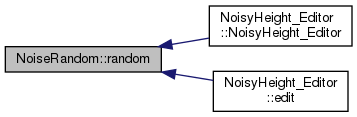
\includegraphics[width=340pt]{namespace_noise_random_a9830d40f986d564ef30504f8dfb9ed90_icgraph}
\end{center}
\end{figure}

\chapter{Documentation des classes}
\hypertarget{class_camera}{}\section{Référence de la classe Camera}
\label{class_camera}\index{Camera@{Camera}}


{\ttfamily \#include $<$camera.\+h$>$}



Graphe d\textquotesingle{}héritage de Camera\+:
\nopagebreak
\begin{figure}[H]
\begin{center}
\leavevmode
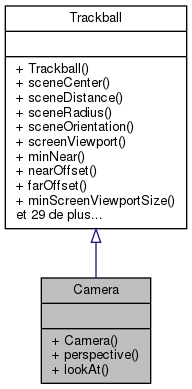
\includegraphics[width=216pt]{class_camera__inherit__graph}
\end{center}
\end{figure}


Graphe de collaboration de Camera\+:
\nopagebreak
\begin{figure}[H]
\begin{center}
\leavevmode
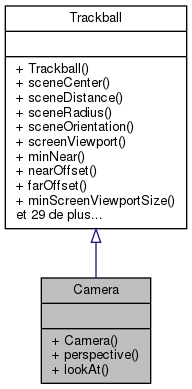
\includegraphics[width=216pt]{class_camera__coll__graph}
\end{center}
\end{figure}
\subsection*{Fonctions membres publiques}
\begin{DoxyCompactItemize}
\item 
\hyperlink{class_camera_a01f94c3543f56ede7af49dc778f19331}{Camera} ()
\end{DoxyCompactItemize}
\subsection*{Fonctions membres publiques statiques}
\begin{DoxyCompactItemize}
\item 
static Eigen\+::\+Matrix4f \hyperlink{class_camera_aa63f48a3280871eba3a6f74a3c0f2e2e}{perspective} (float fovy, float aspect, float z\+Near, float z\+Far)
\item 
static Eigen\+::\+Matrix4f \hyperlink{class_camera_a683a2e432969a485412c28e18567c174}{look\+At} (const Eigen\+::\+Vector3f \&position, const Eigen\+::\+Vector3f \&target, const Eigen\+::\+Vector3f \&up)
\end{DoxyCompactItemize}
\subsection*{Membres hérités additionnels}


\subsection{Documentation des constructeurs et destructeur}
\mbox{\Hypertarget{class_camera_a01f94c3543f56ede7af49dc778f19331}\label{class_camera_a01f94c3543f56ede7af49dc778f19331}} 
\index{Camera@{Camera}!Camera@{Camera}}
\index{Camera@{Camera}!Camera@{Camera}}
\subsubsection{\texorpdfstring{Camera()}{Camera()}}
{\footnotesize\ttfamily Camera\+::\+Camera (\begin{DoxyParamCaption}{ }\end{DoxyParamCaption})\hspace{0.3cm}{\ttfamily [inline]}}

Voici le graphe d\textquotesingle{}appel pour cette fonction \+:\nopagebreak
\begin{figure}[H]
\begin{center}
\leavevmode
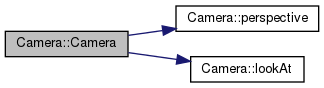
\includegraphics[width=315pt]{class_camera_a01f94c3543f56ede7af49dc778f19331_cgraph}
\end{center}
\end{figure}


\subsection{Documentation des fonctions membres}
\mbox{\Hypertarget{class_camera_a683a2e432969a485412c28e18567c174}\label{class_camera_a683a2e432969a485412c28e18567c174}} 
\index{Camera@{Camera}!look\+At@{look\+At}}
\index{look\+At@{look\+At}!Camera@{Camera}}
\subsubsection{\texorpdfstring{look\+At()}{lookAt()}}
{\footnotesize\ttfamily Matrix4f Camera\+::look\+At (\begin{DoxyParamCaption}\item[{const Eigen\+::\+Vector3f \&}]{position,  }\item[{const Eigen\+::\+Vector3f \&}]{target,  }\item[{const Eigen\+::\+Vector3f \&}]{up }\end{DoxyParamCaption})\hspace{0.3cm}{\ttfamily [static]}}

Voici le graphe des appelants de cette fonction \+:\nopagebreak
\begin{figure}[H]
\begin{center}
\leavevmode
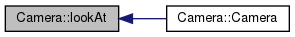
\includegraphics[width=293pt]{class_camera_a683a2e432969a485412c28e18567c174_icgraph}
\end{center}
\end{figure}
\mbox{\Hypertarget{class_camera_aa63f48a3280871eba3a6f74a3c0f2e2e}\label{class_camera_aa63f48a3280871eba3a6f74a3c0f2e2e}} 
\index{Camera@{Camera}!perspective@{perspective}}
\index{perspective@{perspective}!Camera@{Camera}}
\subsubsection{\texorpdfstring{perspective()}{perspective()}}
{\footnotesize\ttfamily Matrix4f Camera\+::perspective (\begin{DoxyParamCaption}\item[{float}]{fovy,  }\item[{float}]{aspect,  }\item[{float}]{z\+Near,  }\item[{float}]{z\+Far }\end{DoxyParamCaption})\hspace{0.3cm}{\ttfamily [static]}}

Voici le graphe des appelants de cette fonction \+:\nopagebreak
\begin{figure}[H]
\begin{center}
\leavevmode
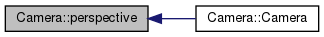
\includegraphics[width=315pt]{class_camera_aa63f48a3280871eba3a6f74a3c0f2e2e_icgraph}
\end{center}
\end{figure}


La documentation de cette classe a été générée à partir des fichiers suivants \+:\begin{DoxyCompactItemize}
\item 
/home/marc-\/cerutti/\+Documents/pdp-\/21-\/2/src/include/\hyperlink{camera_8h}{camera.\+h}\item 
/home/marc-\/cerutti/\+Documents/pdp-\/21-\/2/src/view/\hyperlink{camera_8cpp}{camera.\+cpp}\end{DoxyCompactItemize}

\hypertarget{class_editor}{}\section{Référence de la classe Editor}
\label{class_editor}\index{Editor@{Editor}}


Interface to be implemented by an editor that will transform a generic basic shape into a planet.  




{\ttfamily \#include $<$editor.\+h$>$}



Graphe d\textquotesingle{}héritage de Editor\+:
\nopagebreak
\begin{figure}[H]
\begin{center}
\leavevmode
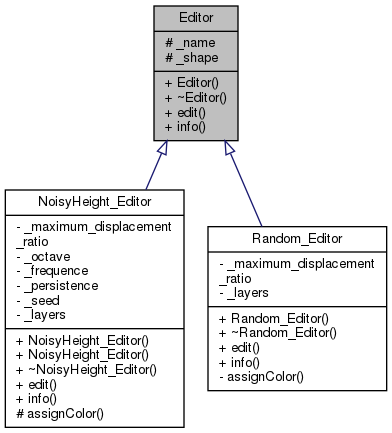
\includegraphics[width=350pt]{class_editor__inherit__graph}
\end{center}
\end{figure}


Graphe de collaboration de Editor\+:\nopagebreak
\begin{figure}[H]
\begin{center}
\leavevmode
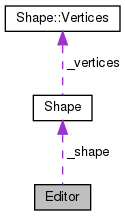
\includegraphics[width=217pt]{class_editor__coll__graph}
\end{center}
\end{figure}
\subsection*{Fonctions membres publiques}
\begin{DoxyCompactItemize}
\item 
\hyperlink{class_editor_aea7f803e3bbb79dbbeb9a9ad9b01ed5a}{Editor} (\hyperlink{class_shape}{Shape} $\ast$shape)
\item 
virtual \hyperlink{class_editor_a192c911dff4ebca89d0b1bb3aa482253}{$\sim$\+Editor} ()=default
\item 
virtual void \hyperlink{class_editor_abca97ba11536c494a0c26bac77917792}{edit} ()=0
\begin{DoxyCompactList}\small\item\em Applies vertex deplacement and colors the shapes. \end{DoxyCompactList}\item 
virtual std\+::string \hyperlink{class_editor_a5747cd74b71d67f6d39b094071058382}{info} () const
\begin{DoxyCompactList}\small\item\em info \end{DoxyCompactList}\end{DoxyCompactItemize}
\subsection*{Attributs protégés}
\begin{DoxyCompactItemize}
\item 
std\+::string \hyperlink{class_editor_a0ae04e135284b48561a538397106f42a}{\+\_\+name}
\item 
\hyperlink{class_shape}{Shape} $\ast$ \hyperlink{class_editor_ad9f31fcae91fb4a91b5ff5ecb4308bdf}{\+\_\+shape}
\end{DoxyCompactItemize}


\subsection{Description détaillée}
Interface to be implemented by an editor that will transform a generic basic shape into a planet. 

\subsection{Documentation des constructeurs et destructeur}
\mbox{\Hypertarget{class_editor_aea7f803e3bbb79dbbeb9a9ad9b01ed5a}\label{class_editor_aea7f803e3bbb79dbbeb9a9ad9b01ed5a}} 
\index{Editor@{Editor}!Editor@{Editor}}
\index{Editor@{Editor}!Editor@{Editor}}
\subsubsection{\texorpdfstring{Editor()}{Editor()}}
{\footnotesize\ttfamily Editor\+::\+Editor (\begin{DoxyParamCaption}\item[{\hyperlink{class_shape}{Shape} $\ast$}]{shape }\end{DoxyParamCaption})\hspace{0.3cm}{\ttfamily [inline]}}

Voici le graphe d\textquotesingle{}appel pour cette fonction \+:\nopagebreak
\begin{figure}[H]
\begin{center}
\leavevmode
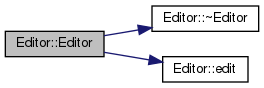
\includegraphics[width=270pt]{class_editor_aea7f803e3bbb79dbbeb9a9ad9b01ed5a_cgraph}
\end{center}
\end{figure}
\mbox{\Hypertarget{class_editor_a192c911dff4ebca89d0b1bb3aa482253}\label{class_editor_a192c911dff4ebca89d0b1bb3aa482253}} 
\index{Editor@{Editor}!````~Editor@{$\sim$\+Editor}}
\index{````~Editor@{$\sim$\+Editor}!Editor@{Editor}}
\subsubsection{\texorpdfstring{$\sim$\+Editor()}{~Editor()}}
{\footnotesize\ttfamily virtual Editor\+::$\sim$\+Editor (\begin{DoxyParamCaption}{ }\end{DoxyParamCaption})\hspace{0.3cm}{\ttfamily [virtual]}, {\ttfamily [default]}}

Voici le graphe des appelants de cette fonction \+:\nopagebreak
\begin{figure}[H]
\begin{center}
\leavevmode
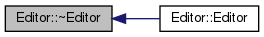
\includegraphics[width=270pt]{class_editor_a192c911dff4ebca89d0b1bb3aa482253_icgraph}
\end{center}
\end{figure}


\subsection{Documentation des fonctions membres}
\mbox{\Hypertarget{class_editor_abca97ba11536c494a0c26bac77917792}\label{class_editor_abca97ba11536c494a0c26bac77917792}} 
\index{Editor@{Editor}!edit@{edit}}
\index{edit@{edit}!Editor@{Editor}}
\subsubsection{\texorpdfstring{edit()}{edit()}}
{\footnotesize\ttfamily virtual void Editor\+::edit (\begin{DoxyParamCaption}{ }\end{DoxyParamCaption})\hspace{0.3cm}{\ttfamily [pure virtual]}}



Applies vertex deplacement and colors the shapes. 



Implémenté dans \hyperlink{class_noisy_height___editor_a3ed5c7267dec56ff2f21366ce2ae9818}{Noisy\+Height\+\_\+\+Editor}, et \hyperlink{class_random___editor_abea41199b1502f89be0b2914b3c191fc}{Random\+\_\+\+Editor}.

Voici le graphe des appelants de cette fonction \+:
\nopagebreak
\begin{figure}[H]
\begin{center}
\leavevmode
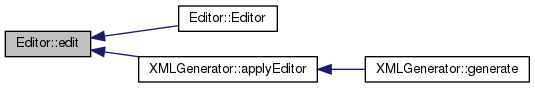
\includegraphics[width=350pt]{class_editor_abca97ba11536c494a0c26bac77917792_icgraph}
\end{center}
\end{figure}
\mbox{\Hypertarget{class_editor_a5747cd74b71d67f6d39b094071058382}\label{class_editor_a5747cd74b71d67f6d39b094071058382}} 
\index{Editor@{Editor}!info@{info}}
\index{info@{info}!Editor@{Editor}}
\subsubsection{\texorpdfstring{info()}{info()}}
{\footnotesize\ttfamily virtual std\+::string Editor\+::info (\begin{DoxyParamCaption}{ }\end{DoxyParamCaption}) const\hspace{0.3cm}{\ttfamily [inline]}, {\ttfamily [virtual]}}



info 

\begin{DoxyReturn}{Renvoie}
the informations of editors, overload it to display parameters informations. 
\end{DoxyReturn}


Réimplémentée dans \hyperlink{class_noisy_height___editor_a4749fe8cb3306252a8f48c8147854578}{Noisy\+Height\+\_\+\+Editor}, et \hyperlink{class_random___editor_aa194991b2926aeab96ad5470f549f087}{Random\+\_\+\+Editor}.

Voici le graphe des appelants de cette fonction \+:
\nopagebreak
\begin{figure}[H]
\begin{center}
\leavevmode
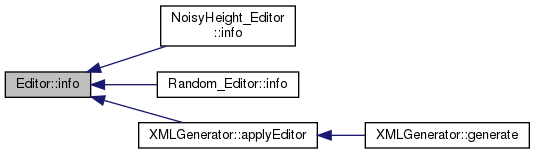
\includegraphics[width=350pt]{class_editor_a5747cd74b71d67f6d39b094071058382_icgraph}
\end{center}
\end{figure}


\subsection{Documentation des données membres}
\mbox{\Hypertarget{class_editor_a0ae04e135284b48561a538397106f42a}\label{class_editor_a0ae04e135284b48561a538397106f42a}} 
\index{Editor@{Editor}!\+\_\+name@{\+\_\+name}}
\index{\+\_\+name@{\+\_\+name}!Editor@{Editor}}
\subsubsection{\texorpdfstring{\+\_\+name}{\_name}}
{\footnotesize\ttfamily std\+::string Editor\+::\+\_\+name\hspace{0.3cm}{\ttfamily [protected]}}

\mbox{\Hypertarget{class_editor_ad9f31fcae91fb4a91b5ff5ecb4308bdf}\label{class_editor_ad9f31fcae91fb4a91b5ff5ecb4308bdf}} 
\index{Editor@{Editor}!\+\_\+shape@{\+\_\+shape}}
\index{\+\_\+shape@{\+\_\+shape}!Editor@{Editor}}
\subsubsection{\texorpdfstring{\+\_\+shape}{\_shape}}
{\footnotesize\ttfamily \hyperlink{class_shape}{Shape}$\ast$ Editor\+::\+\_\+shape\hspace{0.3cm}{\ttfamily [protected]}}



La documentation de cette classe a été générée à partir du fichier suivant \+:\begin{DoxyCompactItemize}
\item 
/home/marc-\/cerutti/\+Documents/pdp-\/21-\/2/src/include/\hyperlink{editor_8h}{editor.\+h}\end{DoxyCompactItemize}

\hypertarget{class_generator}{}\section{Référence de la classe Generator}
\label{class_generator}\index{Generator@{Generator}}


The \hyperlink{class_generator}{Generator} class, permit to read a given configuration file and generate a planet.  




{\ttfamily \#include $<$generator.\+h$>$}



Graphe d\textquotesingle{}héritage de Generator\+:
\nopagebreak
\begin{figure}[H]
\begin{center}
\leavevmode
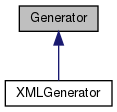
\includegraphics[width=217pt]{class_generator__inherit__graph}
\end{center}
\end{figure}


Graphe de collaboration de Generator\+:\nopagebreak
\begin{figure}[H]
\begin{center}
\leavevmode
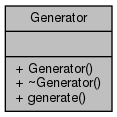
\includegraphics[width=160pt]{class_generator__coll__graph}
\end{center}
\end{figure}
\subsection*{Fonctions membres publiques}
\begin{DoxyCompactItemize}
\item 
\hyperlink{class_generator_aae25f1e872541b353e40fb0e4ee0dd45}{Generator} ()=default
\item 
virtual \hyperlink{class_generator_a175792ff2622a6ce48bf2adab7e09e58}{$\sim$\+Generator} ()=default
\item 
virtual \hyperlink{class_shape}{Shape} $\ast$ \hyperlink{class_generator_a0a421843bba544df32c3e10478eaabc7}{generate} (const std\+::string \&fileconfig)=0
\begin{DoxyCompactList}\small\item\em generate a planet while reading a configuration file. \end{DoxyCompactList}\end{DoxyCompactItemize}


\subsection{Description détaillée}
The \hyperlink{class_generator}{Generator} class, permit to read a given configuration file and generate a planet. 

\subsection{Documentation des constructeurs et destructeur}
\mbox{\Hypertarget{class_generator_aae25f1e872541b353e40fb0e4ee0dd45}\label{class_generator_aae25f1e872541b353e40fb0e4ee0dd45}} 
\index{Generator@{Generator}!Generator@{Generator}}
\index{Generator@{Generator}!Generator@{Generator}}
\subsubsection{\texorpdfstring{Generator()}{Generator()}}
{\footnotesize\ttfamily Generator\+::\+Generator (\begin{DoxyParamCaption}{ }\end{DoxyParamCaption})\hspace{0.3cm}{\ttfamily [default]}}

\mbox{\Hypertarget{class_generator_a175792ff2622a6ce48bf2adab7e09e58}\label{class_generator_a175792ff2622a6ce48bf2adab7e09e58}} 
\index{Generator@{Generator}!````~Generator@{$\sim$\+Generator}}
\index{````~Generator@{$\sim$\+Generator}!Generator@{Generator}}
\subsubsection{\texorpdfstring{$\sim$\+Generator()}{~Generator()}}
{\footnotesize\ttfamily virtual Generator\+::$\sim$\+Generator (\begin{DoxyParamCaption}{ }\end{DoxyParamCaption})\hspace{0.3cm}{\ttfamily [virtual]}, {\ttfamily [default]}}



\subsection{Documentation des fonctions membres}
\mbox{\Hypertarget{class_generator_a0a421843bba544df32c3e10478eaabc7}\label{class_generator_a0a421843bba544df32c3e10478eaabc7}} 
\index{Generator@{Generator}!generate@{generate}}
\index{generate@{generate}!Generator@{Generator}}
\subsubsection{\texorpdfstring{generate()}{generate()}}
{\footnotesize\ttfamily virtual \hyperlink{class_shape}{Shape}$\ast$ Generator\+::generate (\begin{DoxyParamCaption}\item[{const std\+::string \&}]{fileconfig }\end{DoxyParamCaption})\hspace{0.3cm}{\ttfamily [pure virtual]}}



generate a planet while reading a configuration file. 


\begin{DoxyParams}{Paramètres}
{\em fileconfig} & the path to the configuration file. \\
\hline
\end{DoxyParams}
\begin{DoxyReturn}{Renvoie}
Shape$\ast$ the planet allocated, must be free whent not needed anymore. 
\end{DoxyReturn}


Implémenté dans \hyperlink{class_x_m_l_generator_adf874b492da2e813980151c3453dd75c}{X\+M\+L\+Generator}.



La documentation de cette classe a été générée à partir du fichier suivant \+:\begin{DoxyCompactItemize}
\item 
/home/marc-\/cerutti/\+Documents/pdp-\/21-\/2/src/include/\hyperlink{generator_8h}{generator.\+h}\end{DoxyCompactItemize}

\hypertarget{class_noise_random_1_1_height_noise}{}\section{Référence de la classe Noise\+Random\+:\+:Height\+Noise}
\label{class_noise_random_1_1_height_noise}\index{Noise\+Random\+::\+Height\+Noise@{Noise\+Random\+::\+Height\+Noise}}


The \hyperlink{class_noise_random_1_1_height_noise}{Height\+Noise} class generate noise.  




{\ttfamily \#include $<$noiserandom.\+h$>$}



Graphe de collaboration de Noise\+Random\+:\+:Height\+Noise\+:\nopagebreak
\begin{figure}[H]
\begin{center}
\leavevmode
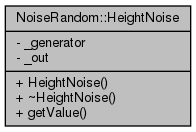
\includegraphics[width=219pt]{class_noise_random_1_1_height_noise__coll__graph}
\end{center}
\end{figure}
\subsection*{Fonctions membres publiques}
\begin{DoxyCompactItemize}
\item 
\hyperlink{class_noise_random_1_1_height_noise_ab166c1a0af9e801a289d33a6d7bd2292}{Height\+Noise} (int seed, double frequence, int octave, double persistence)
\begin{DoxyCompactList}\small\item\em Construct a new Height Noise object. \end{DoxyCompactList}\item 
\hyperlink{class_noise_random_1_1_height_noise_a85d91613d7cc310e928f136680afff22}{$\sim$\+Height\+Noise} ()
\item 
double \hyperlink{class_noise_random_1_1_height_noise_a2fd30f88b20ba463d156c210ef08d54e}{get\+Value} (const Eigen\+::\+Vector3f \&keygen) const
\begin{DoxyCompactList}\small\item\em get\+Value get the value noise. \end{DoxyCompactList}\end{DoxyCompactItemize}
\subsection*{Attributs privés}
\begin{DoxyCompactItemize}
\item 
noise\+::module\+::\+Perlin \hyperlink{class_noise_random_1_1_height_noise_a537d769e59cef8e6691238c9f838510f}{\+\_\+generator}
\item 
noise\+::module\+::\+Clamp \hyperlink{class_noise_random_1_1_height_noise_a5e4713b2a4522778d1478cdf75339658}{\+\_\+out}
\end{DoxyCompactItemize}


\subsection{Description détaillée}
The \hyperlink{class_noise_random_1_1_height_noise}{Height\+Noise} class generate noise. 

\subsection{Documentation des constructeurs et destructeur}
\mbox{\Hypertarget{class_noise_random_1_1_height_noise_ab166c1a0af9e801a289d33a6d7bd2292}\label{class_noise_random_1_1_height_noise_ab166c1a0af9e801a289d33a6d7bd2292}} 
\index{Noise\+Random\+::\+Height\+Noise@{Noise\+Random\+::\+Height\+Noise}!Height\+Noise@{Height\+Noise}}
\index{Height\+Noise@{Height\+Noise}!Noise\+Random\+::\+Height\+Noise@{Noise\+Random\+::\+Height\+Noise}}
\subsubsection{\texorpdfstring{Height\+Noise()}{HeightNoise()}}
{\footnotesize\ttfamily Height\+Noise\+::\+Height\+Noise (\begin{DoxyParamCaption}\item[{int}]{seed,  }\item[{double}]{frequence,  }\item[{int}]{octave,  }\item[{double}]{persistence }\end{DoxyParamCaption})}



Construct a new Height Noise object. 


\begin{DoxyParams}{Paramètres}
{\em seed} & the seed for aleatory. \\
\hline
{\em frequence} & the frerquence of the noise. \\
\hline
{\em octave} & the octave of the noise. \\
\hline
{\em persistence} & the persistence of the noise. More informations for parameters in library libnoise. \\
\hline
\end{DoxyParams}
\mbox{\Hypertarget{class_noise_random_1_1_height_noise_a85d91613d7cc310e928f136680afff22}\label{class_noise_random_1_1_height_noise_a85d91613d7cc310e928f136680afff22}} 
\index{Noise\+Random\+::\+Height\+Noise@{Noise\+Random\+::\+Height\+Noise}!````~Height\+Noise@{$\sim$\+Height\+Noise}}
\index{````~Height\+Noise@{$\sim$\+Height\+Noise}!Noise\+Random\+::\+Height\+Noise@{Noise\+Random\+::\+Height\+Noise}}
\subsubsection{\texorpdfstring{$\sim$\+Height\+Noise()}{~HeightNoise()}}
{\footnotesize\ttfamily Height\+Noise\+::$\sim$\+Height\+Noise (\begin{DoxyParamCaption}{ }\end{DoxyParamCaption})}



\subsection{Documentation des fonctions membres}
\mbox{\Hypertarget{class_noise_random_1_1_height_noise_a2fd30f88b20ba463d156c210ef08d54e}\label{class_noise_random_1_1_height_noise_a2fd30f88b20ba463d156c210ef08d54e}} 
\index{Noise\+Random\+::\+Height\+Noise@{Noise\+Random\+::\+Height\+Noise}!get\+Value@{get\+Value}}
\index{get\+Value@{get\+Value}!Noise\+Random\+::\+Height\+Noise@{Noise\+Random\+::\+Height\+Noise}}
\subsubsection{\texorpdfstring{get\+Value()}{getValue()}}
{\footnotesize\ttfamily double Height\+Noise\+::get\+Value (\begin{DoxyParamCaption}\item[{const Eigen\+::\+Vector3f \&}]{keygen }\end{DoxyParamCaption}) const}



get\+Value get the value noise. 


\begin{DoxyParams}{Paramètres}
{\em keygen} & Tke key for generation. Same key = same value. \\
\hline
\end{DoxyParams}
\begin{DoxyReturn}{Renvoie}
the value noise in double associated to the key. Domain between \mbox{[}-\/1, 1\mbox{]} 
\end{DoxyReturn}
Voici le graphe des appelants de cette fonction \+:\nopagebreak
\begin{figure}[H]
\begin{center}
\leavevmode
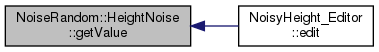
\includegraphics[width=350pt]{class_noise_random_1_1_height_noise_a2fd30f88b20ba463d156c210ef08d54e_icgraph}
\end{center}
\end{figure}


\subsection{Documentation des données membres}
\mbox{\Hypertarget{class_noise_random_1_1_height_noise_a537d769e59cef8e6691238c9f838510f}\label{class_noise_random_1_1_height_noise_a537d769e59cef8e6691238c9f838510f}} 
\index{Noise\+Random\+::\+Height\+Noise@{Noise\+Random\+::\+Height\+Noise}!\+\_\+generator@{\+\_\+generator}}
\index{\+\_\+generator@{\+\_\+generator}!Noise\+Random\+::\+Height\+Noise@{Noise\+Random\+::\+Height\+Noise}}
\subsubsection{\texorpdfstring{\+\_\+generator}{\_generator}}
{\footnotesize\ttfamily noise\+::module\+::\+Perlin Noise\+Random\+::\+Height\+Noise\+::\+\_\+generator\hspace{0.3cm}{\ttfamily [private]}}

\mbox{\Hypertarget{class_noise_random_1_1_height_noise_a5e4713b2a4522778d1478cdf75339658}\label{class_noise_random_1_1_height_noise_a5e4713b2a4522778d1478cdf75339658}} 
\index{Noise\+Random\+::\+Height\+Noise@{Noise\+Random\+::\+Height\+Noise}!\+\_\+out@{\+\_\+out}}
\index{\+\_\+out@{\+\_\+out}!Noise\+Random\+::\+Height\+Noise@{Noise\+Random\+::\+Height\+Noise}}
\subsubsection{\texorpdfstring{\+\_\+out}{\_out}}
{\footnotesize\ttfamily noise\+::module\+::\+Clamp Noise\+Random\+::\+Height\+Noise\+::\+\_\+out\hspace{0.3cm}{\ttfamily [private]}}



La documentation de cette classe a été générée à partir des fichiers suivants \+:\begin{DoxyCompactItemize}
\item 
/home/marc-\/cerutti/\+Documents/pdp-\/21-\/2/src/include/\hyperlink{noiserandom_8h}{noiserandom.\+h}\item 
/home/marc-\/cerutti/\+Documents/pdp-\/21-\/2/src/model/\hyperlink{noiserandom_8cpp}{noiserandom.\+cpp}\end{DoxyCompactItemize}

\hypertarget{class_icosphere}{}\section{Référence de la classe Icosphere}
\label{class_icosphere}\index{Icosphere@{Icosphere}}


Implementation of \hyperlink{class_shape}{Shape} interface.  




{\ttfamily \#include $<$icosphere.\+h$>$}



Graphe d\textquotesingle{}héritage de Icosphere\+:
\nopagebreak
\begin{figure}[H]
\begin{center}
\leavevmode
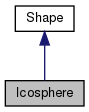
\includegraphics[width=242pt]{class_icosphere__inherit__graph}
\end{center}
\end{figure}


Graphe de collaboration de Icosphere\+:
\nopagebreak
\begin{figure}[H]
\begin{center}
\leavevmode
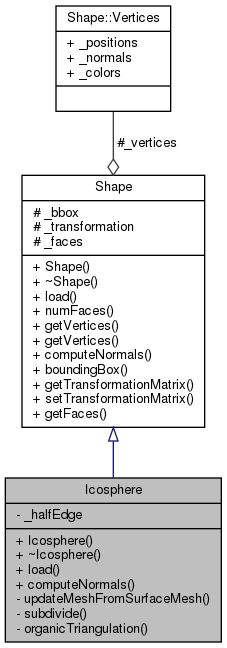
\includegraphics[height=550pt]{class_icosphere__coll__graph}
\end{center}
\end{figure}
\subsection*{Fonctions membres publiques}
\begin{DoxyCompactItemize}
\item 
\hyperlink{class_icosphere_a6051bb79f73f5aecb95074118fb019b3}{Icosphere} (unsigned int nb\+Subdivision, bool organic\+Look=false)
\begin{DoxyCompactList}\small\item\em Construct a new \hyperlink{class_icosphere}{Icosphere} object. \end{DoxyCompactList}\item 
\hyperlink{class_icosphere_ac9473c8c8d6085b6370d95772b898a45}{$\sim$\+Icosphere} ()
\item 
virtual void \hyperlink{class_icosphere_a72c3cc3d95cf508a623fe336cbbab350}{load} (const std\+::string \&filename) override
\begin{DoxyCompactList}\small\item\em Creates the \+\_\+half\+Edge attribute from an O\+BJ file. \end{DoxyCompactList}\item 
virtual void \hyperlink{class_icosphere_af7d6c8c60248794f6a6c382dc5f98a24}{compute\+Normals} () override
\begin{DoxyCompactList}\small\item\em Compute normal for each face. \end{DoxyCompactList}\end{DoxyCompactItemize}
\subsection*{Fonctions membres privées}
\begin{DoxyCompactItemize}
\item 
void \hyperlink{class_icosphere_a38645b095ea6895c2aa5bbff7d8edf20}{update\+Mesh\+From\+Surface\+Mesh} ()
\begin{DoxyCompactList}\small\item\em Updates mesh\textquotesingle{}s attributes (vertices and faces) from its Surface\+\_\+mesh. \end{DoxyCompactList}\item 
void \hyperlink{class_icosphere_a1086e13d1300ed79bf201d2570eb7ebe}{subdivide} ()
\begin{DoxyCompactList}\small\item\em Subdivides the triangluar mesh. Each triangle is subdivided into 4 smaller triangles which allow the mesh to look smoother. \end{DoxyCompactList}\item 
void \hyperlink{class_icosphere_ab3470de718fee359ef4691e0c2ee987a}{organic\+Triangulation} ()
\begin{DoxyCompactList}\small\item\em Move vertices positions to make the planet look more organic. \end{DoxyCompactList}\end{DoxyCompactItemize}
\subsection*{Attributs privés}
\begin{DoxyCompactItemize}
\item 
surface\+\_\+mesh\+::\+Surface\+\_\+mesh \hyperlink{class_icosphere_a454cb570544ec34a65e2f3753fd3dc14}{\+\_\+half\+Edge}
\begin{DoxyCompactList}\small\item\em \+\_\+half\+Edge \+: structure used to know the connectivity between the different faces and vertices. \end{DoxyCompactList}\end{DoxyCompactItemize}
\subsection*{Membres hérités additionnels}


\subsection{Description détaillée}
Implementation of \hyperlink{class_shape}{Shape} interface. 

\subsection{Documentation des constructeurs et destructeur}
\mbox{\Hypertarget{class_icosphere_a6051bb79f73f5aecb95074118fb019b3}\label{class_icosphere_a6051bb79f73f5aecb95074118fb019b3}} 
\index{Icosphere@{Icosphere}!Icosphere@{Icosphere}}
\index{Icosphere@{Icosphere}!Icosphere@{Icosphere}}
\subsubsection{\texorpdfstring{Icosphere()}{Icosphere()}}
{\footnotesize\ttfamily Icosphere\+::\+Icosphere (\begin{DoxyParamCaption}\item[{unsigned int}]{nb\+Subdivision,  }\item[{bool}]{organic\+Look = {\ttfamily false} }\end{DoxyParamCaption})}



Construct a new \hyperlink{class_icosphere}{Icosphere} object. 


\begin{DoxyParams}{Paramètres}
{\em nb\+Subdivision} & the number of subdivision. Higher it is, higher number of polygons it have. Don\textquotesingle{}t use it higher than 10 because of performances issues. \\
\hline
{\em organic\+Look} & permit to displace vertices for a more organic mesh. \\
\hline
\end{DoxyParams}
\mbox{\Hypertarget{class_icosphere_ac9473c8c8d6085b6370d95772b898a45}\label{class_icosphere_ac9473c8c8d6085b6370d95772b898a45}} 
\index{Icosphere@{Icosphere}!````~Icosphere@{$\sim$\+Icosphere}}
\index{````~Icosphere@{$\sim$\+Icosphere}!Icosphere@{Icosphere}}
\subsubsection{\texorpdfstring{$\sim$\+Icosphere()}{~Icosphere()}}
{\footnotesize\ttfamily Icosphere\+::$\sim$\+Icosphere (\begin{DoxyParamCaption}{ }\end{DoxyParamCaption})}



\subsection{Documentation des fonctions membres}
\mbox{\Hypertarget{class_icosphere_af7d6c8c60248794f6a6c382dc5f98a24}\label{class_icosphere_af7d6c8c60248794f6a6c382dc5f98a24}} 
\index{Icosphere@{Icosphere}!compute\+Normals@{compute\+Normals}}
\index{compute\+Normals@{compute\+Normals}!Icosphere@{Icosphere}}
\subsubsection{\texorpdfstring{compute\+Normals()}{computeNormals()}}
{\footnotesize\ttfamily void Icosphere\+::compute\+Normals (\begin{DoxyParamCaption}{ }\end{DoxyParamCaption})\hspace{0.3cm}{\ttfamily [override]}, {\ttfamily [virtual]}}



Compute normal for each face. 



Implémente \hyperlink{class_shape_afd886ad433d08a566003073bfd837f40}{Shape}.

\mbox{\Hypertarget{class_icosphere_a72c3cc3d95cf508a623fe336cbbab350}\label{class_icosphere_a72c3cc3d95cf508a623fe336cbbab350}} 
\index{Icosphere@{Icosphere}!load@{load}}
\index{load@{load}!Icosphere@{Icosphere}}
\subsubsection{\texorpdfstring{load()}{load()}}
{\footnotesize\ttfamily void Icosphere\+::load (\begin{DoxyParamCaption}\item[{const std\+::string \&}]{filename }\end{DoxyParamCaption})\hspace{0.3cm}{\ttfamily [override]}, {\ttfamily [virtual]}}



Creates the \+\_\+half\+Edge attribute from an O\+BJ file. 


\begin{DoxyParams}{Paramètres}
{\em filename} & Path to the file to load \\
\hline
\end{DoxyParams}


Implémente \hyperlink{class_shape_a20d654ec232b682c36cd8b28d2cba750}{Shape}.

\mbox{\Hypertarget{class_icosphere_ab3470de718fee359ef4691e0c2ee987a}\label{class_icosphere_ab3470de718fee359ef4691e0c2ee987a}} 
\index{Icosphere@{Icosphere}!organic\+Triangulation@{organic\+Triangulation}}
\index{organic\+Triangulation@{organic\+Triangulation}!Icosphere@{Icosphere}}
\subsubsection{\texorpdfstring{organic\+Triangulation()}{organicTriangulation()}}
{\footnotesize\ttfamily void Icosphere\+::organic\+Triangulation (\begin{DoxyParamCaption}{ }\end{DoxyParamCaption})\hspace{0.3cm}{\ttfamily [private]}}



Move vertices positions to make the planet look more organic. 

\mbox{\Hypertarget{class_icosphere_a1086e13d1300ed79bf201d2570eb7ebe}\label{class_icosphere_a1086e13d1300ed79bf201d2570eb7ebe}} 
\index{Icosphere@{Icosphere}!subdivide@{subdivide}}
\index{subdivide@{subdivide}!Icosphere@{Icosphere}}
\subsubsection{\texorpdfstring{subdivide()}{subdivide()}}
{\footnotesize\ttfamily void Icosphere\+::subdivide (\begin{DoxyParamCaption}{ }\end{DoxyParamCaption})\hspace{0.3cm}{\ttfamily [private]}}



Subdivides the triangluar mesh. Each triangle is subdivided into 4 smaller triangles which allow the mesh to look smoother. 

The algorithm is from \+: \href{https://www.labri.fr/perso/pbenard/teaching/mondes3d/td9.html}{\tt https\+://www.\+labri.\+fr/perso/pbenard/teaching/mondes3d/td9.\+html} which is based on the thesis \+: \href{https://www.microsoft.com/en-us/research/wp-content/uploads/2016/02/thesis-10.pdf}{\tt https\+://www.\+microsoft.\+com/en-\/us/research/wp-\/content/uploads/2016/02/thesis-\/10.\+pdf}

Step 1 \+: after defining a new Surface\+\_\+mesh, it inserts the vertices of the old one. Then, it adds the intermediate vertices (Ui) on the edges of each triangles \+: \begin{DoxyVerb}                V1- - -U5- - V3
               /  \         /
              /    \       /
             U2     U1    U3
            /        \   /
           /          \ /
         V0- - -U4- - -V2
\end{DoxyVerb}


with the formula \+: U1 = (3/8)$\ast$\+V0+(3/8)$\ast$\+V2+(1/8)$\ast$\+V1+(1/8)$\ast$\+V3 (see above links)

Step 2 \+: it adds the 4 new sub triangles to the new Surface\+\_\+mesh \begin{DoxyVerb}                          V1
                         /  \
                        /    \
                       U0- - -U1
                      /  \   / \
                     /    \ /   \
                   V0- - -U2- - -V2
\end{DoxyVerb}


Step 3 \+: it computes the new positions of the initial vertices \+: \begin{DoxyVerb}                                 di
     Vi' = (1 - B*di) * Vi + B * ∑(Vij)   (see above links)
                                j=1
\end{DoxyVerb}


Step 4 \+: it replaces the old Surface\+\_\+mesh by the new one, and updates the attributes of the mesh from it \mbox{\Hypertarget{class_icosphere_a38645b095ea6895c2aa5bbff7d8edf20}\label{class_icosphere_a38645b095ea6895c2aa5bbff7d8edf20}} 
\index{Icosphere@{Icosphere}!update\+Mesh\+From\+Surface\+Mesh@{update\+Mesh\+From\+Surface\+Mesh}}
\index{update\+Mesh\+From\+Surface\+Mesh@{update\+Mesh\+From\+Surface\+Mesh}!Icosphere@{Icosphere}}
\subsubsection{\texorpdfstring{update\+Mesh\+From\+Surface\+Mesh()}{updateMeshFromSurfaceMesh()}}
{\footnotesize\ttfamily void Icosphere\+::update\+Mesh\+From\+Surface\+Mesh (\begin{DoxyParamCaption}{ }\end{DoxyParamCaption})\hspace{0.3cm}{\ttfamily [private]}}



Updates mesh\textquotesingle{}s attributes (vertices and faces) from its Surface\+\_\+mesh. 



\subsection{Documentation des données membres}
\mbox{\Hypertarget{class_icosphere_a454cb570544ec34a65e2f3753fd3dc14}\label{class_icosphere_a454cb570544ec34a65e2f3753fd3dc14}} 
\index{Icosphere@{Icosphere}!\+\_\+half\+Edge@{\+\_\+half\+Edge}}
\index{\+\_\+half\+Edge@{\+\_\+half\+Edge}!Icosphere@{Icosphere}}
\subsubsection{\texorpdfstring{\+\_\+half\+Edge}{\_halfEdge}}
{\footnotesize\ttfamily surface\+\_\+mesh\+::\+Surface\+\_\+mesh Icosphere\+::\+\_\+half\+Edge\hspace{0.3cm}{\ttfamily [private]}}



\+\_\+half\+Edge \+: structure used to know the connectivity between the different faces and vertices. 



La documentation de cette classe a été générée à partir des fichiers suivants \+:\begin{DoxyCompactItemize}
\item 
/home/marc-\/cerutti/\+Documents/pdp-\/21-\/2/src/include/\hyperlink{icosphere_8h}{icosphere.\+h}\item 
/home/marc-\/cerutti/\+Documents/pdp-\/21-\/2/src/model/\hyperlink{icosphere_8cpp}{icosphere.\+cpp}\end{DoxyCompactItemize}

\hypertarget{class_noisy_height___editor}{}\section{Référence de la classe Noisy\+Height\+\_\+\+Editor}
\label{class_noisy_height___editor}\index{Noisy\+Height\+\_\+\+Editor@{Noisy\+Height\+\_\+\+Editor}}


The \hyperlink{class_noisy_height___editor}{Noisy\+Height\+\_\+\+Editor} class permit to use a noise in order to displace vertices and apply a color from the resulting height.  




{\ttfamily \#include $<$noisyheight\+\_\+editor.\+h$>$}



Graphe d\textquotesingle{}héritage de Noisy\+Height\+\_\+\+Editor\+:\nopagebreak
\begin{figure}[H]
\begin{center}
\leavevmode
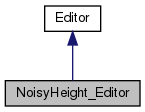
\includegraphics[width=214pt]{class_noisy_height___editor__inherit__graph}
\end{center}
\end{figure}


Graphe de collaboration de Noisy\+Height\+\_\+\+Editor\+:
\nopagebreak
\begin{figure}[H]
\begin{center}
\leavevmode
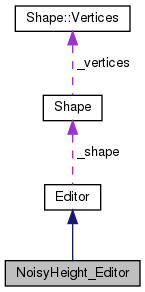
\includegraphics[height=550pt]{class_noisy_height___editor__coll__graph}
\end{center}
\end{figure}
\subsection*{Fonctions membres publiques}
\begin{DoxyCompactItemize}
\item 
\hyperlink{class_noisy_height___editor_ae4535fb17b29bd29d09dcadd5b9384e3}{Noisy\+Height\+\_\+\+Editor} (\hyperlink{class_shape}{Shape} $\ast$shape)
\begin{DoxyCompactList}\small\item\em \hyperlink{class_noisy_height___editor}{Noisy\+Height\+\_\+\+Editor}, default constructor, all parameters random. \end{DoxyCompactList}\item 
\hyperlink{class_noisy_height___editor_ac56426a50e5adf94c8b2a4211d0b0c77}{Noisy\+Height\+\_\+\+Editor} (\hyperlink{class_shape}{Shape} $\ast$shape, double maximum\+\_\+displacement\+\_\+ratio, \hyperlink{aleatorymode_8h_a8dc9582d5186e7d1ba17c0f21779d3d6}{Mode\+\_\+\+Aleatory\+\_\+\+Flags} flags, int octave, double frequence, double persistence, int seed, \hyperlink{thresholdtable_8h_ab0deb49d07758f9814993774cb9935cc}{Color\+Threshold\+Table} $\ast$layers=nullptr)
\begin{DoxyCompactList}\small\item\em \hyperlink{class_noisy_height___editor}{Noisy\+Height\+\_\+\+Editor}. \end{DoxyCompactList}\item 
\hyperlink{class_noisy_height___editor_afd295143a12d4d63773f69c1b5d1318b}{$\sim$\+Noisy\+Height\+\_\+\+Editor} ()
\item 
virtual void \hyperlink{class_noisy_height___editor_a3ed5c7267dec56ff2f21366ce2ae9818}{edit} ()
\begin{DoxyCompactList}\small\item\em Applies vertex deplacement and colors the shapes. \end{DoxyCompactList}\item 
virtual std\+::string \hyperlink{class_noisy_height___editor_a4749fe8cb3306252a8f48c8147854578}{info} () const
\begin{DoxyCompactList}\small\item\em info \end{DoxyCompactList}\end{DoxyCompactItemize}
\subsection*{Fonctions membres protégées}
\begin{DoxyCompactItemize}
\item 
void \hyperlink{class_noisy_height___editor_a4cb46efb3183c7558f450368b962d3fc}{assign\+Color} (\hyperlink{struct_shape_1_1_vertices}{Shape\+::\+Vertices} $\ast$vertices, Eigen\+::\+Vector3f colors)
\end{DoxyCompactItemize}
\subsection*{Attributs privés}
\begin{DoxyCompactItemize}
\item 
double \hyperlink{class_noisy_height___editor_ae4a5069cc1a10e7fd9525648ac20c3b7}{\+\_\+maximum\+\_\+displacement\+\_\+ratio}
\item 
int \hyperlink{class_noisy_height___editor_af52b33d7a5ea98cdda1a1bc17d897d75}{\+\_\+octave}
\item 
double \hyperlink{class_noisy_height___editor_ac6b90169942b0bb92d6461dbf9a2e000}{\+\_\+frequence}
\item 
double \hyperlink{class_noisy_height___editor_aa0752875febd6605a9c0ecdf040c6f48}{\+\_\+persistence}
\item 
int \hyperlink{class_noisy_height___editor_a8765f88743f3ea7f2c850a9415060287}{\+\_\+seed}
\item 
\hyperlink{thresholdtable_8h_ab0deb49d07758f9814993774cb9935cc}{Color\+Threshold\+Table} $\ast$ \hyperlink{class_noisy_height___editor_a40ef1d409c9cbc17b24556b1072e43c1}{\+\_\+layers}
\end{DoxyCompactItemize}
\subsection*{Membres hérités additionnels}


\subsection{Description détaillée}
The \hyperlink{class_noisy_height___editor}{Noisy\+Height\+\_\+\+Editor} class permit to use a noise in order to displace vertices and apply a color from the resulting height. 

\subsection{Documentation des constructeurs et destructeur}
\mbox{\Hypertarget{class_noisy_height___editor_ae4535fb17b29bd29d09dcadd5b9384e3}\label{class_noisy_height___editor_ae4535fb17b29bd29d09dcadd5b9384e3}} 
\index{Noisy\+Height\+\_\+\+Editor@{Noisy\+Height\+\_\+\+Editor}!Noisy\+Height\+\_\+\+Editor@{Noisy\+Height\+\_\+\+Editor}}
\index{Noisy\+Height\+\_\+\+Editor@{Noisy\+Height\+\_\+\+Editor}!Noisy\+Height\+\_\+\+Editor@{Noisy\+Height\+\_\+\+Editor}}
\subsubsection{\texorpdfstring{Noisy\+Height\+\_\+\+Editor()}{NoisyHeight\_Editor()}\hspace{0.1cm}{\footnotesize\ttfamily [1/2]}}
{\footnotesize\ttfamily Noisy\+Height\+\_\+\+Editor\+::\+Noisy\+Height\+\_\+\+Editor (\begin{DoxyParamCaption}\item[{\hyperlink{class_shape}{Shape} $\ast$}]{shape }\end{DoxyParamCaption})}



\hyperlink{class_noisy_height___editor}{Noisy\+Height\+\_\+\+Editor}, default constructor, all parameters random. 


\begin{DoxyParams}{Paramètres}
{\em shape} & the shape to modify. \\
\hline
\end{DoxyParams}
\mbox{\Hypertarget{class_noisy_height___editor_ac56426a50e5adf94c8b2a4211d0b0c77}\label{class_noisy_height___editor_ac56426a50e5adf94c8b2a4211d0b0c77}} 
\index{Noisy\+Height\+\_\+\+Editor@{Noisy\+Height\+\_\+\+Editor}!Noisy\+Height\+\_\+\+Editor@{Noisy\+Height\+\_\+\+Editor}}
\index{Noisy\+Height\+\_\+\+Editor@{Noisy\+Height\+\_\+\+Editor}!Noisy\+Height\+\_\+\+Editor@{Noisy\+Height\+\_\+\+Editor}}
\subsubsection{\texorpdfstring{Noisy\+Height\+\_\+\+Editor()}{NoisyHeight\_Editor()}\hspace{0.1cm}{\footnotesize\ttfamily [2/2]}}
{\footnotesize\ttfamily Noisy\+Height\+\_\+\+Editor\+::\+Noisy\+Height\+\_\+\+Editor (\begin{DoxyParamCaption}\item[{\hyperlink{class_shape}{Shape} $\ast$}]{shape,  }\item[{double}]{maximum\+\_\+displacement\+\_\+ratio,  }\item[{\hyperlink{aleatorymode_8h_a8dc9582d5186e7d1ba17c0f21779d3d6}{Mode\+\_\+\+Aleatory\+\_\+\+Flags}}]{flags,  }\item[{int}]{octave,  }\item[{double}]{frequence,  }\item[{double}]{persistence,  }\item[{int}]{seed,  }\item[{\hyperlink{thresholdtable_8h_ab0deb49d07758f9814993774cb9935cc}{Color\+Threshold\+Table} $\ast$}]{layers = {\ttfamily nullptr} }\end{DoxyParamCaption})}



\hyperlink{class_noisy_height___editor}{Noisy\+Height\+\_\+\+Editor}. 


\begin{DoxyParams}{Paramètres}
{\em shape} & the shape to modify. \\
\hline
{\em maximum\+\_\+displacement\+\_\+ratio} & the maximum displacement factor, determine the height of montains relative to the planet radius. \\
\hline
{\em flags} & the different flags in order to aleatory pick parameters. Combine like for example A\+L\+E\+A\+\_\+\+O\+C\+T\+A\+VE $\vert$ A\+L\+E\+A\+\_\+\+S\+E\+ED. The available for this editor \+: N\+O\+\_\+\+A\+L\+E\+A\+T\+O\+RY A\+L\+E\+A\+\_\+\+O\+C\+T\+A\+VE A\+L\+E\+A\+\_\+\+F\+R\+E\+Q\+U\+E\+N\+CE A\+L\+E\+A\+\_\+\+P\+E\+R\+S\+I\+S\+T\+E\+N\+CE A\+L\+E\+A\+\_\+\+S\+E\+ED \\
\hline
{\em octave} & \\
\hline
{\em frequence} & \\
\hline
{\em persistence} & \\
\hline
{\em seed} & \\
\hline
{\em layers} & the colors with associated bounds of heights. If null, set the default layer for visualisation. Destroyed at the end of life of the object. \\
\hline
\end{DoxyParams}
Voici le graphe d\textquotesingle{}appel pour cette fonction \+:\nopagebreak
\begin{figure}[H]
\begin{center}
\leavevmode
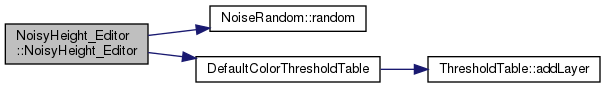
\includegraphics[width=350pt]{class_noisy_height___editor_ac56426a50e5adf94c8b2a4211d0b0c77_cgraph}
\end{center}
\end{figure}
\mbox{\Hypertarget{class_noisy_height___editor_afd295143a12d4d63773f69c1b5d1318b}\label{class_noisy_height___editor_afd295143a12d4d63773f69c1b5d1318b}} 
\index{Noisy\+Height\+\_\+\+Editor@{Noisy\+Height\+\_\+\+Editor}!````~Noisy\+Height\+\_\+\+Editor@{$\sim$\+Noisy\+Height\+\_\+\+Editor}}
\index{````~Noisy\+Height\+\_\+\+Editor@{$\sim$\+Noisy\+Height\+\_\+\+Editor}!Noisy\+Height\+\_\+\+Editor@{Noisy\+Height\+\_\+\+Editor}}
\subsubsection{\texorpdfstring{$\sim$\+Noisy\+Height\+\_\+\+Editor()}{~NoisyHeight\_Editor()}}
{\footnotesize\ttfamily Noisy\+Height\+\_\+\+Editor\+::$\sim$\+Noisy\+Height\+\_\+\+Editor (\begin{DoxyParamCaption}{ }\end{DoxyParamCaption})}



\subsection{Documentation des fonctions membres}
\mbox{\Hypertarget{class_noisy_height___editor_a4cb46efb3183c7558f450368b962d3fc}\label{class_noisy_height___editor_a4cb46efb3183c7558f450368b962d3fc}} 
\index{Noisy\+Height\+\_\+\+Editor@{Noisy\+Height\+\_\+\+Editor}!assign\+Color@{assign\+Color}}
\index{assign\+Color@{assign\+Color}!Noisy\+Height\+\_\+\+Editor@{Noisy\+Height\+\_\+\+Editor}}
\subsubsection{\texorpdfstring{assign\+Color()}{assignColor()}}
{\footnotesize\ttfamily void Noisy\+Height\+\_\+\+Editor\+::assign\+Color (\begin{DoxyParamCaption}\item[{\hyperlink{struct_shape_1_1_vertices}{Shape\+::\+Vertices} $\ast$}]{vertices,  }\item[{Eigen\+::\+Vector3f}]{colors }\end{DoxyParamCaption})\hspace{0.3cm}{\ttfamily [inline]}, {\ttfamily [protected]}}

Voici le graphe des appelants de cette fonction \+:\nopagebreak
\begin{figure}[H]
\begin{center}
\leavevmode
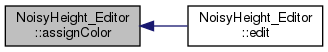
\includegraphics[width=318pt]{class_noisy_height___editor_a4cb46efb3183c7558f450368b962d3fc_icgraph}
\end{center}
\end{figure}
\mbox{\Hypertarget{class_noisy_height___editor_a3ed5c7267dec56ff2f21366ce2ae9818}\label{class_noisy_height___editor_a3ed5c7267dec56ff2f21366ce2ae9818}} 
\index{Noisy\+Height\+\_\+\+Editor@{Noisy\+Height\+\_\+\+Editor}!edit@{edit}}
\index{edit@{edit}!Noisy\+Height\+\_\+\+Editor@{Noisy\+Height\+\_\+\+Editor}}
\subsubsection{\texorpdfstring{edit()}{edit()}}
{\footnotesize\ttfamily void Noisy\+Height\+\_\+\+Editor\+::edit (\begin{DoxyParamCaption}{ }\end{DoxyParamCaption})\hspace{0.3cm}{\ttfamily [virtual]}}



Applies vertex deplacement and colors the shapes. 



Implémente \hyperlink{class_editor_abca97ba11536c494a0c26bac77917792}{Editor}.

Voici le graphe d\textquotesingle{}appel pour cette fonction \+:
\nopagebreak
\begin{figure}[H]
\begin{center}
\leavevmode
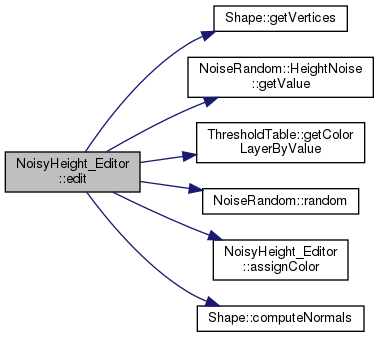
\includegraphics[width=350pt]{class_noisy_height___editor_a3ed5c7267dec56ff2f21366ce2ae9818_cgraph}
\end{center}
\end{figure}
\mbox{\Hypertarget{class_noisy_height___editor_a4749fe8cb3306252a8f48c8147854578}\label{class_noisy_height___editor_a4749fe8cb3306252a8f48c8147854578}} 
\index{Noisy\+Height\+\_\+\+Editor@{Noisy\+Height\+\_\+\+Editor}!info@{info}}
\index{info@{info}!Noisy\+Height\+\_\+\+Editor@{Noisy\+Height\+\_\+\+Editor}}
\subsubsection{\texorpdfstring{info()}{info()}}
{\footnotesize\ttfamily std\+::string Noisy\+Height\+\_\+\+Editor\+::info (\begin{DoxyParamCaption}{ }\end{DoxyParamCaption}) const\hspace{0.3cm}{\ttfamily [virtual]}}



info 

\begin{DoxyReturn}{Renvoie}
the informations of editors, overload it to display parameters informations. 
\end{DoxyReturn}


Réimplémentée à partir de \hyperlink{class_editor_a5747cd74b71d67f6d39b094071058382}{Editor}.

Voici le graphe d\textquotesingle{}appel pour cette fonction \+:\nopagebreak
\begin{figure}[H]
\begin{center}
\leavevmode
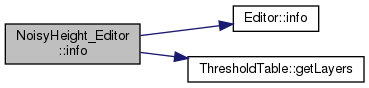
\includegraphics[width=349pt]{class_noisy_height___editor_a4749fe8cb3306252a8f48c8147854578_cgraph}
\end{center}
\end{figure}


\subsection{Documentation des données membres}
\mbox{\Hypertarget{class_noisy_height___editor_ac6b90169942b0bb92d6461dbf9a2e000}\label{class_noisy_height___editor_ac6b90169942b0bb92d6461dbf9a2e000}} 
\index{Noisy\+Height\+\_\+\+Editor@{Noisy\+Height\+\_\+\+Editor}!\+\_\+frequence@{\+\_\+frequence}}
\index{\+\_\+frequence@{\+\_\+frequence}!Noisy\+Height\+\_\+\+Editor@{Noisy\+Height\+\_\+\+Editor}}
\subsubsection{\texorpdfstring{\+\_\+frequence}{\_frequence}}
{\footnotesize\ttfamily double Noisy\+Height\+\_\+\+Editor\+::\+\_\+frequence\hspace{0.3cm}{\ttfamily [private]}}

\mbox{\Hypertarget{class_noisy_height___editor_a40ef1d409c9cbc17b24556b1072e43c1}\label{class_noisy_height___editor_a40ef1d409c9cbc17b24556b1072e43c1}} 
\index{Noisy\+Height\+\_\+\+Editor@{Noisy\+Height\+\_\+\+Editor}!\+\_\+layers@{\+\_\+layers}}
\index{\+\_\+layers@{\+\_\+layers}!Noisy\+Height\+\_\+\+Editor@{Noisy\+Height\+\_\+\+Editor}}
\subsubsection{\texorpdfstring{\+\_\+layers}{\_layers}}
{\footnotesize\ttfamily \hyperlink{thresholdtable_8h_ab0deb49d07758f9814993774cb9935cc}{Color\+Threshold\+Table}$\ast$ Noisy\+Height\+\_\+\+Editor\+::\+\_\+layers\hspace{0.3cm}{\ttfamily [private]}}

\mbox{\Hypertarget{class_noisy_height___editor_ae4a5069cc1a10e7fd9525648ac20c3b7}\label{class_noisy_height___editor_ae4a5069cc1a10e7fd9525648ac20c3b7}} 
\index{Noisy\+Height\+\_\+\+Editor@{Noisy\+Height\+\_\+\+Editor}!\+\_\+maximum\+\_\+displacement\+\_\+ratio@{\+\_\+maximum\+\_\+displacement\+\_\+ratio}}
\index{\+\_\+maximum\+\_\+displacement\+\_\+ratio@{\+\_\+maximum\+\_\+displacement\+\_\+ratio}!Noisy\+Height\+\_\+\+Editor@{Noisy\+Height\+\_\+\+Editor}}
\subsubsection{\texorpdfstring{\+\_\+maximum\+\_\+displacement\+\_\+ratio}{\_maximum\_displacement\_ratio}}
{\footnotesize\ttfamily double Noisy\+Height\+\_\+\+Editor\+::\+\_\+maximum\+\_\+displacement\+\_\+ratio\hspace{0.3cm}{\ttfamily [private]}}

\mbox{\Hypertarget{class_noisy_height___editor_af52b33d7a5ea98cdda1a1bc17d897d75}\label{class_noisy_height___editor_af52b33d7a5ea98cdda1a1bc17d897d75}} 
\index{Noisy\+Height\+\_\+\+Editor@{Noisy\+Height\+\_\+\+Editor}!\+\_\+octave@{\+\_\+octave}}
\index{\+\_\+octave@{\+\_\+octave}!Noisy\+Height\+\_\+\+Editor@{Noisy\+Height\+\_\+\+Editor}}
\subsubsection{\texorpdfstring{\+\_\+octave}{\_octave}}
{\footnotesize\ttfamily int Noisy\+Height\+\_\+\+Editor\+::\+\_\+octave\hspace{0.3cm}{\ttfamily [private]}}

\mbox{\Hypertarget{class_noisy_height___editor_aa0752875febd6605a9c0ecdf040c6f48}\label{class_noisy_height___editor_aa0752875febd6605a9c0ecdf040c6f48}} 
\index{Noisy\+Height\+\_\+\+Editor@{Noisy\+Height\+\_\+\+Editor}!\+\_\+persistence@{\+\_\+persistence}}
\index{\+\_\+persistence@{\+\_\+persistence}!Noisy\+Height\+\_\+\+Editor@{Noisy\+Height\+\_\+\+Editor}}
\subsubsection{\texorpdfstring{\+\_\+persistence}{\_persistence}}
{\footnotesize\ttfamily double Noisy\+Height\+\_\+\+Editor\+::\+\_\+persistence\hspace{0.3cm}{\ttfamily [private]}}

\mbox{\Hypertarget{class_noisy_height___editor_a8765f88743f3ea7f2c850a9415060287}\label{class_noisy_height___editor_a8765f88743f3ea7f2c850a9415060287}} 
\index{Noisy\+Height\+\_\+\+Editor@{Noisy\+Height\+\_\+\+Editor}!\+\_\+seed@{\+\_\+seed}}
\index{\+\_\+seed@{\+\_\+seed}!Noisy\+Height\+\_\+\+Editor@{Noisy\+Height\+\_\+\+Editor}}
\subsubsection{\texorpdfstring{\+\_\+seed}{\_seed}}
{\footnotesize\ttfamily int Noisy\+Height\+\_\+\+Editor\+::\+\_\+seed\hspace{0.3cm}{\ttfamily [private]}}



La documentation de cette classe a été générée à partir des fichiers suivants \+:\begin{DoxyCompactItemize}
\item 
/home/marc-\/cerutti/\+Documents/pdp-\/21-\/2/src/include/\hyperlink{noisyheight__editor_8h}{noisyheight\+\_\+editor.\+h}\item 
/home/marc-\/cerutti/\+Documents/pdp-\/21-\/2/src/model/\hyperlink{noisyheight__editor_8cpp}{noisyheight\+\_\+editor.\+cpp}\end{DoxyCompactItemize}

\hypertarget{class_random___editor}{}\section{Référence de la classe Random\+\_\+\+Editor}
\label{class_random___editor}\index{Random\+\_\+\+Editor@{Random\+\_\+\+Editor}}


Applies a random modification to the position (x,y,z) of each vertex and applies color depending on the new position. This class allows to transform a generic icosphere into a simple planet.  




{\ttfamily \#include $<$random\+\_\+editor.\+h$>$}



Graphe d\textquotesingle{}héritage de Random\+\_\+\+Editor\+:\nopagebreak
\begin{figure}[H]
\begin{center}
\leavevmode
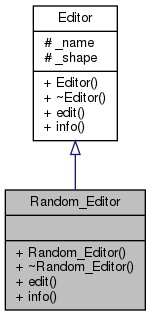
\includegraphics[width=164pt]{class_random___editor__inherit__graph}
\end{center}
\end{figure}


Graphe de collaboration de Random\+\_\+\+Editor\+:\nopagebreak
\begin{figure}[H]
\begin{center}
\leavevmode
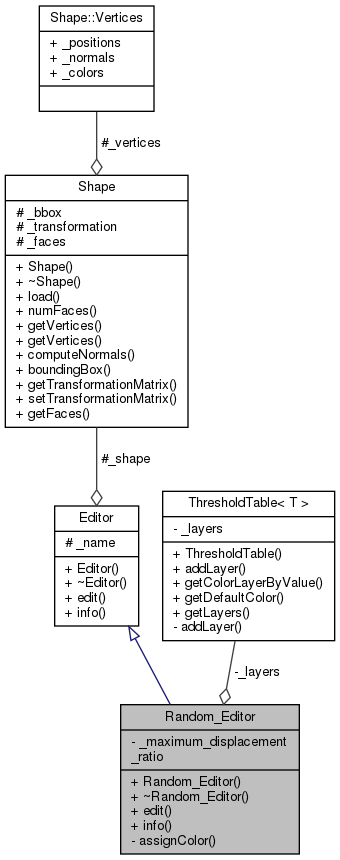
\includegraphics[width=166pt]{class_random___editor__coll__graph}
\end{center}
\end{figure}
\subsection*{Fonctions membres publiques}
\begin{DoxyCompactItemize}
\item 
\hyperlink{class_random___editor_a68118d2b9929e7c9dbb821ce76554164}{Random\+\_\+\+Editor} (\hyperlink{class_shape}{Shape} $\ast$shape, double maximum\+\_\+displacement\+\_\+ratio=\hyperlink{editor_8h_ad4ef0738a1a62405f443237adf55b8c8}{D\+E\+F\+A\+U\+L\+T\+\_\+\+M\+A\+X\+I\+M\+U\+M\+\_\+\+D\+I\+S\+P\+L\+A\+C\+E\+M\+E\+N\+T\+\_\+\+R\+A\+T\+IO}, \hyperlink{thresholdtable_8h_ab0deb49d07758f9814993774cb9935cc}{Color\+Threshold\+Table} $\ast$layers=nullptr)
\begin{DoxyCompactList}\small\item\em \hyperlink{class_random___editor}{Random\+\_\+\+Editor}. \end{DoxyCompactList}\item 
\hyperlink{class_random___editor_a8a062c4450faafac081ff65b7465545d}{$\sim$\+Random\+\_\+\+Editor} ()
\item 
virtual void \hyperlink{class_random___editor_abea41199b1502f89be0b2914b3c191fc}{edit} ()
\begin{DoxyCompactList}\small\item\em Applies vertex deplacement and colors the shape. \end{DoxyCompactList}\item 
virtual std\+::string \hyperlink{class_random___editor_aa194991b2926aeab96ad5470f549f087}{info} () const
\begin{DoxyCompactList}\small\item\em info \end{DoxyCompactList}\end{DoxyCompactItemize}
\subsection*{Membres hérités additionnels}


\subsection{Description détaillée}
Applies a random modification to the position (x,y,z) of each vertex and applies color depending on the new position. This class allows to transform a generic icosphere into a simple planet. 

\subsection{Documentation des constructeurs et destructeur}
\mbox{\Hypertarget{class_random___editor_a68118d2b9929e7c9dbb821ce76554164}\label{class_random___editor_a68118d2b9929e7c9dbb821ce76554164}} 
\index{Random\+\_\+\+Editor@{Random\+\_\+\+Editor}!Random\+\_\+\+Editor@{Random\+\_\+\+Editor}}
\index{Random\+\_\+\+Editor@{Random\+\_\+\+Editor}!Random\+\_\+\+Editor@{Random\+\_\+\+Editor}}
\subsubsection{\texorpdfstring{Random\+\_\+\+Editor()}{Random\_Editor()}}
{\footnotesize\ttfamily Random\+\_\+\+Editor\+::\+Random\+\_\+\+Editor (\begin{DoxyParamCaption}\item[{\hyperlink{class_shape}{Shape} $\ast$}]{shape,  }\item[{double}]{maximum\+\_\+displacement\+\_\+ratio = {\ttfamily \hyperlink{editor_8h_ad4ef0738a1a62405f443237adf55b8c8}{D\+E\+F\+A\+U\+L\+T\+\_\+\+M\+A\+X\+I\+M\+U\+M\+\_\+\+D\+I\+S\+P\+L\+A\+C\+E\+M\+E\+N\+T\+\_\+\+R\+A\+T\+IO}},  }\item[{\hyperlink{thresholdtable_8h_ab0deb49d07758f9814993774cb9935cc}{Color\+Threshold\+Table} $\ast$}]{layers = {\ttfamily nullptr} }\end{DoxyParamCaption})}



\hyperlink{class_random___editor}{Random\+\_\+\+Editor}. 


\begin{DoxyParams}{Paramètres}
{\em shape} & the shpe to modify. \\
\hline
{\em maximum\+\_\+displacement\+\_\+ratio} & the maximum displacement. \\
\hline
{\em layers} & the colors with associated bounds of heights. \\
\hline
\end{DoxyParams}
Voici le graphe d\textquotesingle{}appel pour cette fonction \+:\nopagebreak
\begin{figure}[H]
\begin{center}
\leavevmode
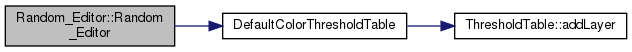
\includegraphics[width=350pt]{class_random___editor_a68118d2b9929e7c9dbb821ce76554164_cgraph}
\end{center}
\end{figure}
\mbox{\Hypertarget{class_random___editor_a8a062c4450faafac081ff65b7465545d}\label{class_random___editor_a8a062c4450faafac081ff65b7465545d}} 
\index{Random\+\_\+\+Editor@{Random\+\_\+\+Editor}!````~Random\+\_\+\+Editor@{$\sim$\+Random\+\_\+\+Editor}}
\index{````~Random\+\_\+\+Editor@{$\sim$\+Random\+\_\+\+Editor}!Random\+\_\+\+Editor@{Random\+\_\+\+Editor}}
\subsubsection{\texorpdfstring{$\sim$\+Random\+\_\+\+Editor()}{~Random\_Editor()}}
{\footnotesize\ttfamily Random\+\_\+\+Editor\+::$\sim$\+Random\+\_\+\+Editor (\begin{DoxyParamCaption}{ }\end{DoxyParamCaption})}



\subsection{Documentation des fonctions membres}
\mbox{\Hypertarget{class_random___editor_abea41199b1502f89be0b2914b3c191fc}\label{class_random___editor_abea41199b1502f89be0b2914b3c191fc}} 
\index{Random\+\_\+\+Editor@{Random\+\_\+\+Editor}!edit@{edit}}
\index{edit@{edit}!Random\+\_\+\+Editor@{Random\+\_\+\+Editor}}
\subsubsection{\texorpdfstring{edit()}{edit()}}
{\footnotesize\ttfamily void Random\+\_\+\+Editor\+::edit (\begin{DoxyParamCaption}{ }\end{DoxyParamCaption})\hspace{0.3cm}{\ttfamily [virtual]}}



Applies vertex deplacement and colors the shape. 



Implémente \hyperlink{class_editor_abca97ba11536c494a0c26bac77917792}{Editor}.

Voici le graphe d\textquotesingle{}appel pour cette fonction \+:\nopagebreak
\begin{figure}[H]
\begin{center}
\leavevmode
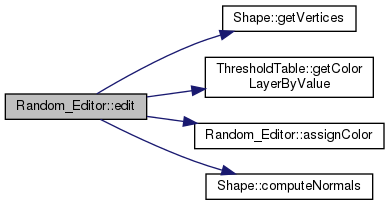
\includegraphics[width=348pt]{class_random___editor_abea41199b1502f89be0b2914b3c191fc_cgraph}
\end{center}
\end{figure}
\mbox{\Hypertarget{class_random___editor_aa194991b2926aeab96ad5470f549f087}\label{class_random___editor_aa194991b2926aeab96ad5470f549f087}} 
\index{Random\+\_\+\+Editor@{Random\+\_\+\+Editor}!info@{info}}
\index{info@{info}!Random\+\_\+\+Editor@{Random\+\_\+\+Editor}}
\subsubsection{\texorpdfstring{info()}{info()}}
{\footnotesize\ttfamily std\+::string Random\+\_\+\+Editor\+::info (\begin{DoxyParamCaption}{ }\end{DoxyParamCaption}) const\hspace{0.3cm}{\ttfamily [virtual]}}



info 

\begin{DoxyReturn}{Renvoie}
the informations of editors, overload it to display parameters informations. 
\end{DoxyReturn}


Réimplémentée à partir de \hyperlink{class_editor_a5747cd74b71d67f6d39b094071058382}{Editor}.

Voici le graphe d\textquotesingle{}appel pour cette fonction \+:\nopagebreak
\begin{figure}[H]
\begin{center}
\leavevmode
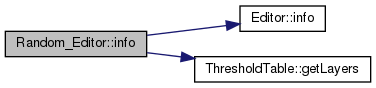
\includegraphics[width=350pt]{class_random___editor_aa194991b2926aeab96ad5470f549f087_cgraph}
\end{center}
\end{figure}


La documentation de cette classe a été générée à partir des fichiers suivants \+:\begin{DoxyCompactItemize}
\item 
/home/marc-\/cerutti/\+Documents/pdp-\/21-\/2/src/include/\hyperlink{random__editor_8h}{random\+\_\+editor.\+h}\item 
/home/marc-\/cerutti/\+Documents/pdp-\/21-\/2/src/model/\hyperlink{random__editor_8cpp}{random\+\_\+editor.\+cpp}\end{DoxyCompactItemize}

\hypertarget{class_rendering}{}\section{Référence de la classe Rendering}
\label{class_rendering}\index{Rendering@{Rendering}}


Interface of Bridge pattern use to free the dependance with library like open\+GL.  




{\ttfamily \#include $<$rendering.\+h$>$}



Graphe d\textquotesingle{}héritage de Rendering\+:
\nopagebreak
\begin{figure}[H]
\begin{center}
\leavevmode
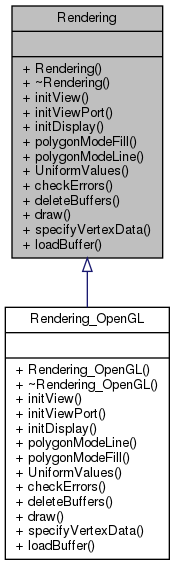
\includegraphics[width=203pt]{class_rendering__inherit__graph}
\end{center}
\end{figure}


Graphe de collaboration de Rendering\+:\nopagebreak
\begin{figure}[H]
\begin{center}
\leavevmode
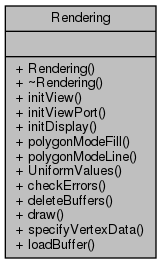
\includegraphics[width=193pt]{class_rendering__coll__graph}
\end{center}
\end{figure}
\subsection*{Fonctions membres publiques}
\begin{DoxyCompactItemize}
\item 
\hyperlink{class_rendering_a2d6135f6f0563031d59f12e81c15416d}{Rendering} ()
\item 
virtual \hyperlink{class_rendering_aefe02eb379fb45f7270bd0887c6c3d5e}{$\sim$\+Rendering} ()
\item 
virtual void \hyperlink{class_rendering_abf05def5b7eb02669008cf44c3520dae}{init\+View} ()=0
\begin{DoxyCompactList}\small\item\em initialize View \end{DoxyCompactList}\item 
virtual void \hyperlink{class_rendering_a87a6dd12561315a07ec111ea2939a3c2}{init\+View\+Port} (int x, int y, int w, int h)=0
\begin{DoxyCompactList}\small\item\em initialize Viewport \end{DoxyCompactList}\item 
virtual void \hyperlink{class_rendering_ae3ad4a7f4c5559cb258d72886123c3e0}{init\+Display} ()=0
\begin{DoxyCompactList}\small\item\em initialize Display \end{DoxyCompactList}\item 
virtual void \hyperlink{class_rendering_a9ea983c02e590c78d564908d6171335e}{polygon\+Mode\+Fill} ()=0
\begin{DoxyCompactList}\small\item\em Switch to polygone mode fill. \end{DoxyCompactList}\item 
virtual void \hyperlink{class_rendering_aeb3922ecc539c6d8e9339fb3760cd560}{polygon\+Mode\+Line} ()=0
\begin{DoxyCompactList}\small\item\em Switch to polygone mode line. \end{DoxyCompactList}\item 
virtual void \hyperlink{class_rendering_a09a77bbedf75aff7535c419b6f8e4915}{Uniform\+Values} (\hyperlink{class_shader}{Shader} $\ast$shader, \hyperlink{class_trackball}{Trackball} cam, Eigen\+::\+Vector3f light\+Dir, Eigen\+::\+Matrix3f normal, Eigen\+::\+Matrix4f model, int sea\+\_\+mode)=0
\begin{DoxyCompactList}\small\item\em Uniform values for renderer. \end{DoxyCompactList}\item 
virtual void \hyperlink{class_rendering_a93693702cf5a7709a7b1ddc7a7d3d8d3}{check\+Errors} ()=0
\begin{DoxyCompactList}\small\item\em check errors \end{DoxyCompactList}\item 
virtual void \hyperlink{class_rendering_a43cc4c8b7b4d9813773b42c97a7405d5}{delete\+Buffers} ()=0
\begin{DoxyCompactList}\small\item\em delete buffers \end{DoxyCompactList}\item 
virtual void \hyperlink{class_rendering_abeffb3c261cd9b5c6b885aaf8e321ef2}{draw} (int nb\+\_\+elements, \hyperlink{class_shader}{Shader} $\ast$shader)=0
\begin{DoxyCompactList}\small\item\em Draws the data computed init. \end{DoxyCompactList}\item 
virtual void \hyperlink{class_rendering_aecb85f0a1da2d14cde84a918e2636841}{specify\+Vertex\+Data} (\hyperlink{class_shader}{Shader} $\ast$shader)=0
\begin{DoxyCompactList}\small\item\em Sends vertices data to the shader. \end{DoxyCompactList}\item 
virtual void \hyperlink{class_rendering_aa753ed0c94b2ece92afd26a58aef4f79}{load\+Buffer} (const \hyperlink{struct_shape_1_1_vertices}{Shape\+::\+Vertices} $\ast$vertices, std\+::vector$<$ Eigen\+::\+Vector3i $>$ faces)=0
\begin{DoxyCompactList}\small\item\em Computes all the data needed by Open\+GL for the display (\+\_\+positions,\+\_\+normals,\+\_\+colors,\+\_\+indices) \end{DoxyCompactList}\end{DoxyCompactItemize}


\subsection{Description détaillée}
Interface of Bridge pattern use to free the dependance with library like open\+GL. 

\subsection{Documentation des constructeurs et destructeur}
\mbox{\Hypertarget{class_rendering_a2d6135f6f0563031d59f12e81c15416d}\label{class_rendering_a2d6135f6f0563031d59f12e81c15416d}} 
\index{Rendering@{Rendering}!Rendering@{Rendering}}
\index{Rendering@{Rendering}!Rendering@{Rendering}}
\subsubsection{\texorpdfstring{Rendering()}{Rendering()}}
{\footnotesize\ttfamily Rendering\+::\+Rendering (\begin{DoxyParamCaption}{ }\end{DoxyParamCaption})\hspace{0.3cm}{\ttfamily [inline]}}

\mbox{\Hypertarget{class_rendering_aefe02eb379fb45f7270bd0887c6c3d5e}\label{class_rendering_aefe02eb379fb45f7270bd0887c6c3d5e}} 
\index{Rendering@{Rendering}!````~Rendering@{$\sim$\+Rendering}}
\index{````~Rendering@{$\sim$\+Rendering}!Rendering@{Rendering}}
\subsubsection{\texorpdfstring{$\sim$\+Rendering()}{~Rendering()}}
{\footnotesize\ttfamily virtual Rendering\+::$\sim$\+Rendering (\begin{DoxyParamCaption}{ }\end{DoxyParamCaption})\hspace{0.3cm}{\ttfamily [inline]}, {\ttfamily [virtual]}}

Voici le graphe d\textquotesingle{}appel pour cette fonction \+:\nopagebreak
\begin{figure}[H]
\begin{center}
\leavevmode
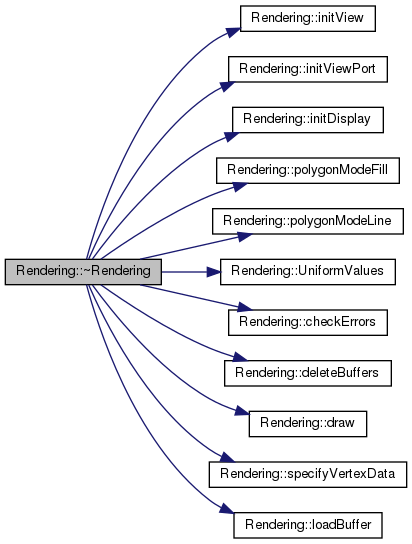
\includegraphics[width=350pt]{class_rendering_aefe02eb379fb45f7270bd0887c6c3d5e_cgraph}
\end{center}
\end{figure}


\subsection{Documentation des fonctions membres}
\mbox{\Hypertarget{class_rendering_a93693702cf5a7709a7b1ddc7a7d3d8d3}\label{class_rendering_a93693702cf5a7709a7b1ddc7a7d3d8d3}} 
\index{Rendering@{Rendering}!check\+Errors@{check\+Errors}}
\index{check\+Errors@{check\+Errors}!Rendering@{Rendering}}
\subsubsection{\texorpdfstring{check\+Errors()}{checkErrors()}}
{\footnotesize\ttfamily virtual void Rendering\+::check\+Errors (\begin{DoxyParamCaption}{ }\end{DoxyParamCaption})\hspace{0.3cm}{\ttfamily [pure virtual]}}



check errors 



Implémenté dans \hyperlink{class_rendering___open_g_l_a9621079239b6b621dfc8f9c4e93bdd7a}{Rendering\+\_\+\+Open\+GL}.

Voici le graphe des appelants de cette fonction \+:\nopagebreak
\begin{figure}[H]
\begin{center}
\leavevmode
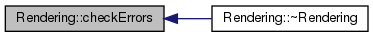
\includegraphics[width=350pt]{class_rendering_a93693702cf5a7709a7b1ddc7a7d3d8d3_icgraph}
\end{center}
\end{figure}
\mbox{\Hypertarget{class_rendering_a43cc4c8b7b4d9813773b42c97a7405d5}\label{class_rendering_a43cc4c8b7b4d9813773b42c97a7405d5}} 
\index{Rendering@{Rendering}!delete\+Buffers@{delete\+Buffers}}
\index{delete\+Buffers@{delete\+Buffers}!Rendering@{Rendering}}
\subsubsection{\texorpdfstring{delete\+Buffers()}{deleteBuffers()}}
{\footnotesize\ttfamily virtual void Rendering\+::delete\+Buffers (\begin{DoxyParamCaption}{ }\end{DoxyParamCaption})\hspace{0.3cm}{\ttfamily [pure virtual]}}



delete buffers 



Implémenté dans \hyperlink{class_rendering___open_g_l_aab5b195bb52751243f4944417f9ae7d5}{Rendering\+\_\+\+Open\+GL}.

Voici le graphe des appelants de cette fonction \+:\nopagebreak
\begin{figure}[H]
\begin{center}
\leavevmode
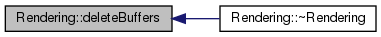
\includegraphics[width=350pt]{class_rendering_a43cc4c8b7b4d9813773b42c97a7405d5_icgraph}
\end{center}
\end{figure}
\mbox{\Hypertarget{class_rendering_abeffb3c261cd9b5c6b885aaf8e321ef2}\label{class_rendering_abeffb3c261cd9b5c6b885aaf8e321ef2}} 
\index{Rendering@{Rendering}!draw@{draw}}
\index{draw@{draw}!Rendering@{Rendering}}
\subsubsection{\texorpdfstring{draw()}{draw()}}
{\footnotesize\ttfamily virtual void Rendering\+::draw (\begin{DoxyParamCaption}\item[{int}]{nb\+\_\+elements,  }\item[{\hyperlink{class_shader}{Shader} $\ast$}]{shader }\end{DoxyParamCaption})\hspace{0.3cm}{\ttfamily [pure virtual]}}



Draws the data computed init. 


\begin{DoxyParams}{Paramètres}
{\em nb\+\_\+elements} & \+: number of elements (faces) to draw \\
\hline
{\em shader} & \+: shader used to draws the data \\
\hline
\end{DoxyParams}


Implémenté dans \hyperlink{class_rendering___open_g_l_a94abb636d4264637628e4b9b97c087d2}{Rendering\+\_\+\+Open\+GL}.

Voici le graphe des appelants de cette fonction \+:\nopagebreak
\begin{figure}[H]
\begin{center}
\leavevmode
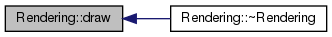
\includegraphics[width=321pt]{class_rendering_abeffb3c261cd9b5c6b885aaf8e321ef2_icgraph}
\end{center}
\end{figure}
\mbox{\Hypertarget{class_rendering_ae3ad4a7f4c5559cb258d72886123c3e0}\label{class_rendering_ae3ad4a7f4c5559cb258d72886123c3e0}} 
\index{Rendering@{Rendering}!init\+Display@{init\+Display}}
\index{init\+Display@{init\+Display}!Rendering@{Rendering}}
\subsubsection{\texorpdfstring{init\+Display()}{initDisplay()}}
{\footnotesize\ttfamily virtual void Rendering\+::init\+Display (\begin{DoxyParamCaption}{ }\end{DoxyParamCaption})\hspace{0.3cm}{\ttfamily [pure virtual]}}



initialize Display 



Implémenté dans \hyperlink{class_rendering___open_g_l_a2df315de627ccedc056c5834e65bda6d}{Rendering\+\_\+\+Open\+GL}.

Voici le graphe des appelants de cette fonction \+:\nopagebreak
\begin{figure}[H]
\begin{center}
\leavevmode
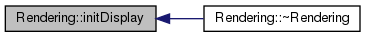
\includegraphics[width=346pt]{class_rendering_ae3ad4a7f4c5559cb258d72886123c3e0_icgraph}
\end{center}
\end{figure}
\mbox{\Hypertarget{class_rendering_abf05def5b7eb02669008cf44c3520dae}\label{class_rendering_abf05def5b7eb02669008cf44c3520dae}} 
\index{Rendering@{Rendering}!init\+View@{init\+View}}
\index{init\+View@{init\+View}!Rendering@{Rendering}}
\subsubsection{\texorpdfstring{init\+View()}{initView()}}
{\footnotesize\ttfamily virtual void Rendering\+::init\+View (\begin{DoxyParamCaption}{ }\end{DoxyParamCaption})\hspace{0.3cm}{\ttfamily [pure virtual]}}



initialize View 



Implémenté dans \hyperlink{class_rendering___open_g_l_aa41657730fef1c0034233a9977a31531}{Rendering\+\_\+\+Open\+GL}.

Voici le graphe des appelants de cette fonction \+:\nopagebreak
\begin{figure}[H]
\begin{center}
\leavevmode
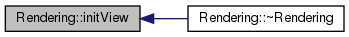
\includegraphics[width=334pt]{class_rendering_abf05def5b7eb02669008cf44c3520dae_icgraph}
\end{center}
\end{figure}
\mbox{\Hypertarget{class_rendering_a87a6dd12561315a07ec111ea2939a3c2}\label{class_rendering_a87a6dd12561315a07ec111ea2939a3c2}} 
\index{Rendering@{Rendering}!init\+View\+Port@{init\+View\+Port}}
\index{init\+View\+Port@{init\+View\+Port}!Rendering@{Rendering}}
\subsubsection{\texorpdfstring{init\+View\+Port()}{initViewPort()}}
{\footnotesize\ttfamily virtual void Rendering\+::init\+View\+Port (\begin{DoxyParamCaption}\item[{int}]{x,  }\item[{int}]{y,  }\item[{int}]{w,  }\item[{int}]{h }\end{DoxyParamCaption})\hspace{0.3cm}{\ttfamily [pure virtual]}}



initialize Viewport 


\begin{DoxyParams}{Paramètres}
{\em x} & \+: abscissa of origin point \\
\hline
{\em y} & \+: ordinate of origin point \\
\hline
{\em w} & \+: width of the window \\
\hline
{\em h} & \+: height of the window \\
\hline
\end{DoxyParams}


Implémenté dans \hyperlink{class_rendering___open_g_l_ac6c10061853d88c1ab6e40d6c172c69c}{Rendering\+\_\+\+Open\+GL}.

Voici le graphe des appelants de cette fonction \+:\nopagebreak
\begin{figure}[H]
\begin{center}
\leavevmode
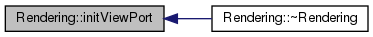
\includegraphics[width=350pt]{class_rendering_a87a6dd12561315a07ec111ea2939a3c2_icgraph}
\end{center}
\end{figure}
\mbox{\Hypertarget{class_rendering_aa753ed0c94b2ece92afd26a58aef4f79}\label{class_rendering_aa753ed0c94b2ece92afd26a58aef4f79}} 
\index{Rendering@{Rendering}!load\+Buffer@{load\+Buffer}}
\index{load\+Buffer@{load\+Buffer}!Rendering@{Rendering}}
\subsubsection{\texorpdfstring{load\+Buffer()}{loadBuffer()}}
{\footnotesize\ttfamily virtual void Rendering\+::load\+Buffer (\begin{DoxyParamCaption}\item[{const \hyperlink{struct_shape_1_1_vertices}{Shape\+::\+Vertices} $\ast$}]{vertices,  }\item[{std\+::vector$<$ Eigen\+::\+Vector3i $>$}]{faces }\end{DoxyParamCaption})\hspace{0.3cm}{\ttfamily [pure virtual]}}



Computes all the data needed by Open\+GL for the display (\+\_\+positions,\+\_\+normals,\+\_\+colors,\+\_\+indices) 


\begin{DoxyParams}{Paramètres}
{\em vertices} & \+: vertices of the shape \\
\hline
{\em faces} & \+: faces of the shape \\
\hline
\end{DoxyParams}


Implémenté dans \hyperlink{class_rendering___open_g_l_aee7a6085edb4e6927282067b6cde59bf}{Rendering\+\_\+\+Open\+GL}.

Voici le graphe des appelants de cette fonction \+:\nopagebreak
\begin{figure}[H]
\begin{center}
\leavevmode
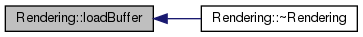
\includegraphics[width=344pt]{class_rendering_aa753ed0c94b2ece92afd26a58aef4f79_icgraph}
\end{center}
\end{figure}
\mbox{\Hypertarget{class_rendering_a9ea983c02e590c78d564908d6171335e}\label{class_rendering_a9ea983c02e590c78d564908d6171335e}} 
\index{Rendering@{Rendering}!polygon\+Mode\+Fill@{polygon\+Mode\+Fill}}
\index{polygon\+Mode\+Fill@{polygon\+Mode\+Fill}!Rendering@{Rendering}}
\subsubsection{\texorpdfstring{polygon\+Mode\+Fill()}{polygonModeFill()}}
{\footnotesize\ttfamily virtual void Rendering\+::polygon\+Mode\+Fill (\begin{DoxyParamCaption}{ }\end{DoxyParamCaption})\hspace{0.3cm}{\ttfamily [pure virtual]}}



Switch to polygone mode fill. 



Implémenté dans \hyperlink{class_rendering___open_g_l_a4e3a8195e4249bf0d7c8b33400611399}{Rendering\+\_\+\+Open\+GL}.

Voici le graphe des appelants de cette fonction \+:\nopagebreak
\begin{figure}[H]
\begin{center}
\leavevmode
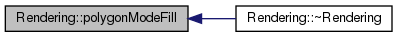
\includegraphics[width=350pt]{class_rendering_a9ea983c02e590c78d564908d6171335e_icgraph}
\end{center}
\end{figure}
\mbox{\Hypertarget{class_rendering_aeb3922ecc539c6d8e9339fb3760cd560}\label{class_rendering_aeb3922ecc539c6d8e9339fb3760cd560}} 
\index{Rendering@{Rendering}!polygon\+Mode\+Line@{polygon\+Mode\+Line}}
\index{polygon\+Mode\+Line@{polygon\+Mode\+Line}!Rendering@{Rendering}}
\subsubsection{\texorpdfstring{polygon\+Mode\+Line()}{polygonModeLine()}}
{\footnotesize\ttfamily virtual void Rendering\+::polygon\+Mode\+Line (\begin{DoxyParamCaption}{ }\end{DoxyParamCaption})\hspace{0.3cm}{\ttfamily [pure virtual]}}



Switch to polygone mode line. 



Implémenté dans \hyperlink{class_rendering___open_g_l_a7742b4b96b3e06a021f143d17fd432df}{Rendering\+\_\+\+Open\+GL}.

Voici le graphe des appelants de cette fonction \+:\nopagebreak
\begin{figure}[H]
\begin{center}
\leavevmode
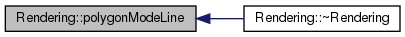
\includegraphics[width=350pt]{class_rendering_aeb3922ecc539c6d8e9339fb3760cd560_icgraph}
\end{center}
\end{figure}
\mbox{\Hypertarget{class_rendering_aecb85f0a1da2d14cde84a918e2636841}\label{class_rendering_aecb85f0a1da2d14cde84a918e2636841}} 
\index{Rendering@{Rendering}!specify\+Vertex\+Data@{specify\+Vertex\+Data}}
\index{specify\+Vertex\+Data@{specify\+Vertex\+Data}!Rendering@{Rendering}}
\subsubsection{\texorpdfstring{specify\+Vertex\+Data()}{specifyVertexData()}}
{\footnotesize\ttfamily virtual void Rendering\+::specify\+Vertex\+Data (\begin{DoxyParamCaption}\item[{\hyperlink{class_shader}{Shader} $\ast$}]{shader }\end{DoxyParamCaption})\hspace{0.3cm}{\ttfamily [pure virtual]}}



Sends vertices data to the shader. 


\begin{DoxyParams}{Paramètres}
{\em shader} & \+: shader used to display the data \\
\hline
\end{DoxyParams}


Implémenté dans \hyperlink{class_rendering___open_g_l_a8ad1a3e698d694782f4174d94b745cd5}{Rendering\+\_\+\+Open\+GL}.

Voici le graphe des appelants de cette fonction \+:\nopagebreak
\begin{figure}[H]
\begin{center}
\leavevmode
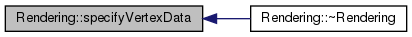
\includegraphics[width=350pt]{class_rendering_aecb85f0a1da2d14cde84a918e2636841_icgraph}
\end{center}
\end{figure}
\mbox{\Hypertarget{class_rendering_a09a77bbedf75aff7535c419b6f8e4915}\label{class_rendering_a09a77bbedf75aff7535c419b6f8e4915}} 
\index{Rendering@{Rendering}!Uniform\+Values@{Uniform\+Values}}
\index{Uniform\+Values@{Uniform\+Values}!Rendering@{Rendering}}
\subsubsection{\texorpdfstring{Uniform\+Values()}{UniformValues()}}
{\footnotesize\ttfamily virtual void Rendering\+::\+Uniform\+Values (\begin{DoxyParamCaption}\item[{\hyperlink{class_shader}{Shader} $\ast$}]{shader,  }\item[{\hyperlink{class_trackball}{Trackball}}]{cam,  }\item[{Eigen\+::\+Vector3f}]{light\+Dir,  }\item[{Eigen\+::\+Matrix3f}]{normal,  }\item[{Eigen\+::\+Matrix4f}]{model,  }\item[{int}]{sea\+\_\+mode }\end{DoxyParamCaption})\hspace{0.3cm}{\ttfamily [pure virtual]}}



Uniform values for renderer. 


\begin{DoxyParams}{Paramètres}
{\em shader} & \+: shader used to draws the data \\
\hline
{\em cam} & \+: camera used for the scene \\
\hline
{\em light\+Dir} & \+: light\textquotesingle{}s direction \\
\hline
{\em normal} & \+: normal\textquotesingle{}s transformation matrix \\
\hline
{\em model} & \+: model\textquotesingle{}s transformation matrix \\
\hline
\end{DoxyParams}


Implémenté dans \hyperlink{class_rendering___open_g_l_a3d370bebbf4e66ba7bd4ea61dc59bef1}{Rendering\+\_\+\+Open\+GL}.

Voici le graphe des appelants de cette fonction \+:\nopagebreak
\begin{figure}[H]
\begin{center}
\leavevmode
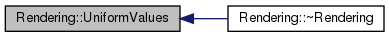
\includegraphics[width=350pt]{class_rendering_a09a77bbedf75aff7535c419b6f8e4915_icgraph}
\end{center}
\end{figure}


La documentation de cette classe a été générée à partir du fichier suivant \+:\begin{DoxyCompactItemize}
\item 
/home/marc-\/cerutti/\+Documents/pdp-\/21-\/2/src/include/\hyperlink{rendering_8h}{rendering.\+h}\end{DoxyCompactItemize}

\hypertarget{class_rendering___open_g_l}{}\section{Référence de la classe Rendering\+\_\+\+Open\+GL}
\label{class_rendering___open_g_l}\index{Rendering\+\_\+\+Open\+GL@{Rendering\+\_\+\+Open\+GL}}


Class implementing \hyperlink{class_rendering}{Rendering}.  




{\ttfamily \#include $<$rendering\+\_\+opengl.\+h$>$}



Graphe d\textquotesingle{}héritage de Rendering\+\_\+\+Open\+GL\+:
\nopagebreak
\begin{figure}[H]
\begin{center}
\leavevmode
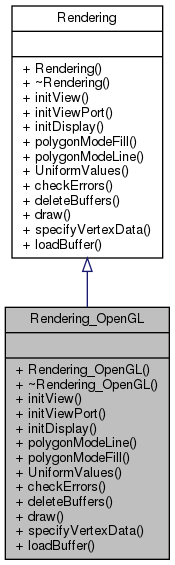
\includegraphics[width=203pt]{class_rendering___open_g_l__inherit__graph}
\end{center}
\end{figure}


Graphe de collaboration de Rendering\+\_\+\+Open\+GL\+:
\nopagebreak
\begin{figure}[H]
\begin{center}
\leavevmode
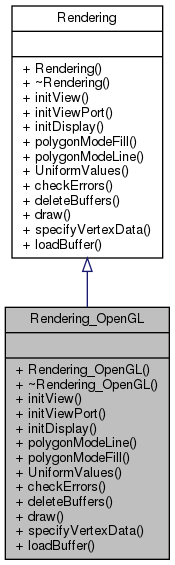
\includegraphics[width=203pt]{class_rendering___open_g_l__coll__graph}
\end{center}
\end{figure}
\subsection*{Fonctions membres publiques}
\begin{DoxyCompactItemize}
\item 
\hyperlink{class_rendering___open_g_l_a0db708eaeae23e85a18d9c40995b27ae}{Rendering\+\_\+\+Open\+GL} ()
\item 
\hyperlink{class_rendering___open_g_l_a32ff44fc5d3a776a6add4eef3f662a96}{$\sim$\+Rendering\+\_\+\+Open\+GL} ()
\item 
void \hyperlink{class_rendering___open_g_l_aa41657730fef1c0034233a9977a31531}{init\+View} ()
\begin{DoxyCompactList}\small\item\em initialize View \end{DoxyCompactList}\item 
void \hyperlink{class_rendering___open_g_l_ac6c10061853d88c1ab6e40d6c172c69c}{init\+View\+Port} (int x, int y, int w, int h)
\begin{DoxyCompactList}\small\item\em initialize Viewport \end{DoxyCompactList}\item 
void \hyperlink{class_rendering___open_g_l_a2df315de627ccedc056c5834e65bda6d}{init\+Display} ()
\begin{DoxyCompactList}\small\item\em initialize Display \end{DoxyCompactList}\item 
void \hyperlink{class_rendering___open_g_l_a7742b4b96b3e06a021f143d17fd432df}{polygon\+Mode\+Line} ()
\begin{DoxyCompactList}\small\item\em Switch to polygone mode line. \end{DoxyCompactList}\item 
void \hyperlink{class_rendering___open_g_l_a4e3a8195e4249bf0d7c8b33400611399}{polygon\+Mode\+Fill} ()
\begin{DoxyCompactList}\small\item\em Switch to polygone mode fill. \end{DoxyCompactList}\item 
void \hyperlink{class_rendering___open_g_l_a3d370bebbf4e66ba7bd4ea61dc59bef1}{Uniform\+Values} (\hyperlink{class_shader}{Shader} $\ast$shader, \hyperlink{class_trackball}{Trackball} cam, Eigen\+::\+Vector3f light\+Dir, Eigen\+::\+Matrix3f normal, Eigen\+::\+Matrix4f model, int sea\+\_\+mode)
\begin{DoxyCompactList}\small\item\em Uniform values for renderer. \end{DoxyCompactList}\item 
void \hyperlink{class_rendering___open_g_l_a9621079239b6b621dfc8f9c4e93bdd7a}{check\+Errors} ()
\begin{DoxyCompactList}\small\item\em check errors \end{DoxyCompactList}\item 
void \hyperlink{class_rendering___open_g_l_aab5b195bb52751243f4944417f9ae7d5}{delete\+Buffers} ()
\begin{DoxyCompactList}\small\item\em delete buffers \end{DoxyCompactList}\item 
void \hyperlink{class_rendering___open_g_l_a94abb636d4264637628e4b9b97c087d2}{draw} (int nb\+\_\+elements, \hyperlink{class_shader}{Shader} $\ast$shader)
\begin{DoxyCompactList}\small\item\em Draws the data computed init. \end{DoxyCompactList}\item 
void \hyperlink{class_rendering___open_g_l_a8ad1a3e698d694782f4174d94b745cd5}{specify\+Vertex\+Data} (\hyperlink{class_shader}{Shader} $\ast$shader)
\begin{DoxyCompactList}\small\item\em Sends vertices data to the shader. \end{DoxyCompactList}\item 
void \hyperlink{class_rendering___open_g_l_aee7a6085edb4e6927282067b6cde59bf}{load\+Buffer} (const \hyperlink{struct_shape_1_1_vertices}{Shape\+::\+Vertices} $\ast$vertices, std\+::vector$<$ Eigen\+::\+Vector3i $>$ faces)
\begin{DoxyCompactList}\small\item\em Computes all the data needed by Open\+GL for the display (\+\_\+positions,\+\_\+normals,\+\_\+colors,\+\_\+indices) \end{DoxyCompactList}\end{DoxyCompactItemize}
\subsection*{Attributs privés}
\begin{DoxyCompactItemize}
\item 
G\+Luint \hyperlink{class_rendering___open_g_l_a6838049f26cc1811531f2e266f61c158}{\+\_\+faces\+Buffer}
\begin{DoxyCompactList}\small\item\em Variables used for open\+GL buffers. \end{DoxyCompactList}\item 
G\+Luint \hyperlink{class_rendering___open_g_l_a4397283457770370db833b1c59db797e}{\+\_\+vao}
\item 
G\+Luint \hyperlink{class_rendering___open_g_l_ade7eb98ac80d30c4611389027a2ed568}{\+\_\+vbo} \mbox{[}3\mbox{]}
\end{DoxyCompactItemize}


\subsection{Description détaillée}
Class implementing \hyperlink{class_rendering}{Rendering}. 

\subsection{Documentation des constructeurs et destructeur}
\mbox{\Hypertarget{class_rendering___open_g_l_a0db708eaeae23e85a18d9c40995b27ae}\label{class_rendering___open_g_l_a0db708eaeae23e85a18d9c40995b27ae}} 
\index{Rendering\+\_\+\+Open\+GL@{Rendering\+\_\+\+Open\+GL}!Rendering\+\_\+\+Open\+GL@{Rendering\+\_\+\+Open\+GL}}
\index{Rendering\+\_\+\+Open\+GL@{Rendering\+\_\+\+Open\+GL}!Rendering\+\_\+\+Open\+GL@{Rendering\+\_\+\+Open\+GL}}
\subsubsection{\texorpdfstring{Rendering\+\_\+\+Open\+G\+L()}{Rendering\_OpenGL()}}
{\footnotesize\ttfamily Rendering\+\_\+\+Open\+G\+L\+::\+Rendering\+\_\+\+Open\+GL (\begin{DoxyParamCaption}{ }\end{DoxyParamCaption})\hspace{0.3cm}{\ttfamily [inline]}}

Voici le graphe d\textquotesingle{}appel pour cette fonction \+:\nopagebreak
\begin{figure}[H]
\begin{center}
\leavevmode
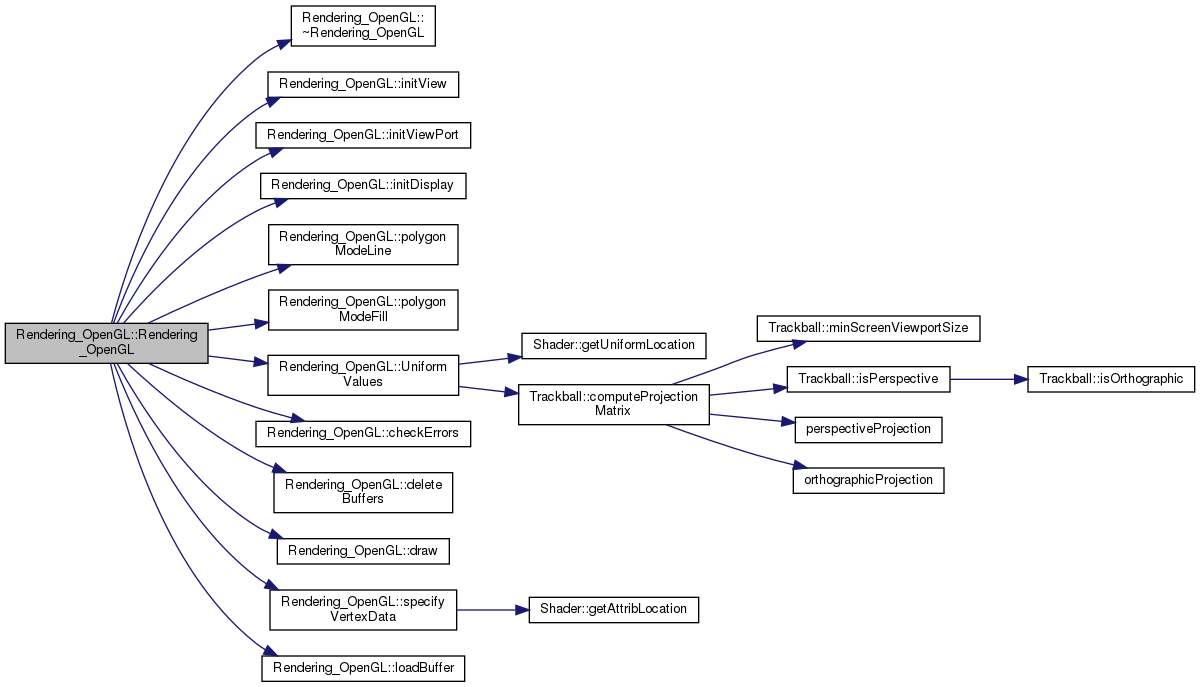
\includegraphics[width=350pt]{class_rendering___open_g_l_a0db708eaeae23e85a18d9c40995b27ae_cgraph}
\end{center}
\end{figure}
\mbox{\Hypertarget{class_rendering___open_g_l_a32ff44fc5d3a776a6add4eef3f662a96}\label{class_rendering___open_g_l_a32ff44fc5d3a776a6add4eef3f662a96}} 
\index{Rendering\+\_\+\+Open\+GL@{Rendering\+\_\+\+Open\+GL}!````~Rendering\+\_\+\+Open\+GL@{$\sim$\+Rendering\+\_\+\+Open\+GL}}
\index{````~Rendering\+\_\+\+Open\+GL@{$\sim$\+Rendering\+\_\+\+Open\+GL}!Rendering\+\_\+\+Open\+GL@{Rendering\+\_\+\+Open\+GL}}
\subsubsection{\texorpdfstring{$\sim$\+Rendering\+\_\+\+Open\+G\+L()}{~Rendering\_OpenGL()}}
{\footnotesize\ttfamily Rendering\+\_\+\+Open\+G\+L\+::$\sim$\+Rendering\+\_\+\+Open\+GL (\begin{DoxyParamCaption}{ }\end{DoxyParamCaption})}

Voici le graphe des appelants de cette fonction \+:\nopagebreak
\begin{figure}[H]
\begin{center}
\leavevmode
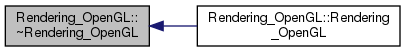
\includegraphics[width=350pt]{class_rendering___open_g_l_a32ff44fc5d3a776a6add4eef3f662a96_icgraph}
\end{center}
\end{figure}


\subsection{Documentation des fonctions membres}
\mbox{\Hypertarget{class_rendering___open_g_l_a9621079239b6b621dfc8f9c4e93bdd7a}\label{class_rendering___open_g_l_a9621079239b6b621dfc8f9c4e93bdd7a}} 
\index{Rendering\+\_\+\+Open\+GL@{Rendering\+\_\+\+Open\+GL}!check\+Errors@{check\+Errors}}
\index{check\+Errors@{check\+Errors}!Rendering\+\_\+\+Open\+GL@{Rendering\+\_\+\+Open\+GL}}
\subsubsection{\texorpdfstring{check\+Errors()}{checkErrors()}}
{\footnotesize\ttfamily void Rendering\+\_\+\+Open\+G\+L\+::check\+Errors (\begin{DoxyParamCaption}{ }\end{DoxyParamCaption})\hspace{0.3cm}{\ttfamily [virtual]}}



check errors 



Implémente \hyperlink{class_rendering_a93693702cf5a7709a7b1ddc7a7d3d8d3}{Rendering}.

Voici le graphe des appelants de cette fonction \+:\nopagebreak
\begin{figure}[H]
\begin{center}
\leavevmode
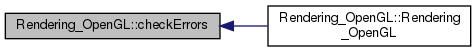
\includegraphics[width=350pt]{class_rendering___open_g_l_a9621079239b6b621dfc8f9c4e93bdd7a_icgraph}
\end{center}
\end{figure}
\mbox{\Hypertarget{class_rendering___open_g_l_aab5b195bb52751243f4944417f9ae7d5}\label{class_rendering___open_g_l_aab5b195bb52751243f4944417f9ae7d5}} 
\index{Rendering\+\_\+\+Open\+GL@{Rendering\+\_\+\+Open\+GL}!delete\+Buffers@{delete\+Buffers}}
\index{delete\+Buffers@{delete\+Buffers}!Rendering\+\_\+\+Open\+GL@{Rendering\+\_\+\+Open\+GL}}
\subsubsection{\texorpdfstring{delete\+Buffers()}{deleteBuffers()}}
{\footnotesize\ttfamily void Rendering\+\_\+\+Open\+G\+L\+::delete\+Buffers (\begin{DoxyParamCaption}{ }\end{DoxyParamCaption})\hspace{0.3cm}{\ttfamily [virtual]}}



delete buffers 



Implémente \hyperlink{class_rendering_a43cc4c8b7b4d9813773b42c97a7405d5}{Rendering}.

Voici le graphe des appelants de cette fonction \+:\nopagebreak
\begin{figure}[H]
\begin{center}
\leavevmode
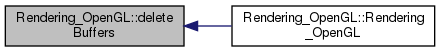
\includegraphics[width=350pt]{class_rendering___open_g_l_aab5b195bb52751243f4944417f9ae7d5_icgraph}
\end{center}
\end{figure}
\mbox{\Hypertarget{class_rendering___open_g_l_a94abb636d4264637628e4b9b97c087d2}\label{class_rendering___open_g_l_a94abb636d4264637628e4b9b97c087d2}} 
\index{Rendering\+\_\+\+Open\+GL@{Rendering\+\_\+\+Open\+GL}!draw@{draw}}
\index{draw@{draw}!Rendering\+\_\+\+Open\+GL@{Rendering\+\_\+\+Open\+GL}}
\subsubsection{\texorpdfstring{draw()}{draw()}}
{\footnotesize\ttfamily void Rendering\+\_\+\+Open\+G\+L\+::draw (\begin{DoxyParamCaption}\item[{int}]{nb\+\_\+elements,  }\item[{\hyperlink{class_shader}{Shader} $\ast$}]{shader }\end{DoxyParamCaption})\hspace{0.3cm}{\ttfamily [virtual]}}



Draws the data computed init. 


\begin{DoxyParams}{Paramètres}
{\em nb\+\_\+elements} & \+: number of elements (faces) to draw \\
\hline
{\em shader} & \+: shader used to draws the data \\
\hline
\end{DoxyParams}


Implémente \hyperlink{class_rendering_abeffb3c261cd9b5c6b885aaf8e321ef2}{Rendering}.

Voici le graphe des appelants de cette fonction \+:\nopagebreak
\begin{figure}[H]
\begin{center}
\leavevmode
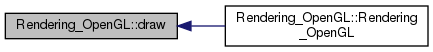
\includegraphics[width=350pt]{class_rendering___open_g_l_a94abb636d4264637628e4b9b97c087d2_icgraph}
\end{center}
\end{figure}
\mbox{\Hypertarget{class_rendering___open_g_l_a2df315de627ccedc056c5834e65bda6d}\label{class_rendering___open_g_l_a2df315de627ccedc056c5834e65bda6d}} 
\index{Rendering\+\_\+\+Open\+GL@{Rendering\+\_\+\+Open\+GL}!init\+Display@{init\+Display}}
\index{init\+Display@{init\+Display}!Rendering\+\_\+\+Open\+GL@{Rendering\+\_\+\+Open\+GL}}
\subsubsection{\texorpdfstring{init\+Display()}{initDisplay()}}
{\footnotesize\ttfamily void Rendering\+\_\+\+Open\+G\+L\+::init\+Display (\begin{DoxyParamCaption}{ }\end{DoxyParamCaption})\hspace{0.3cm}{\ttfamily [virtual]}}



initialize Display 



Implémente \hyperlink{class_rendering_ae3ad4a7f4c5559cb258d72886123c3e0}{Rendering}.

Voici le graphe des appelants de cette fonction \+:\nopagebreak
\begin{figure}[H]
\begin{center}
\leavevmode
\includegraphics[width=350pt]{class_rendering___open_g_l_a2df315de627ccedc056c5834e65bda6d_icgraph}
\end{center}
\end{figure}
\mbox{\Hypertarget{class_rendering___open_g_l_aa41657730fef1c0034233a9977a31531}\label{class_rendering___open_g_l_aa41657730fef1c0034233a9977a31531}} 
\index{Rendering\+\_\+\+Open\+GL@{Rendering\+\_\+\+Open\+GL}!init\+View@{init\+View}}
\index{init\+View@{init\+View}!Rendering\+\_\+\+Open\+GL@{Rendering\+\_\+\+Open\+GL}}
\subsubsection{\texorpdfstring{init\+View()}{initView()}}
{\footnotesize\ttfamily void Rendering\+\_\+\+Open\+G\+L\+::init\+View (\begin{DoxyParamCaption}{ }\end{DoxyParamCaption})\hspace{0.3cm}{\ttfamily [virtual]}}



initialize View 



Implémente \hyperlink{class_rendering_abf05def5b7eb02669008cf44c3520dae}{Rendering}.

Voici le graphe des appelants de cette fonction \+:\nopagebreak
\begin{figure}[H]
\begin{center}
\leavevmode
\includegraphics[width=350pt]{class_rendering___open_g_l_aa41657730fef1c0034233a9977a31531_icgraph}
\end{center}
\end{figure}
\mbox{\Hypertarget{class_rendering___open_g_l_ac6c10061853d88c1ab6e40d6c172c69c}\label{class_rendering___open_g_l_ac6c10061853d88c1ab6e40d6c172c69c}} 
\index{Rendering\+\_\+\+Open\+GL@{Rendering\+\_\+\+Open\+GL}!init\+View\+Port@{init\+View\+Port}}
\index{init\+View\+Port@{init\+View\+Port}!Rendering\+\_\+\+Open\+GL@{Rendering\+\_\+\+Open\+GL}}
\subsubsection{\texorpdfstring{init\+View\+Port()}{initViewPort()}}
{\footnotesize\ttfamily void Rendering\+\_\+\+Open\+G\+L\+::init\+View\+Port (\begin{DoxyParamCaption}\item[{int}]{x,  }\item[{int}]{y,  }\item[{int}]{w,  }\item[{int}]{h }\end{DoxyParamCaption})\hspace{0.3cm}{\ttfamily [virtual]}}



initialize Viewport 


\begin{DoxyParams}{Paramètres}
{\em x} & \+: abscissa of origin point \\
\hline
{\em y} & \+: ordinate of origin point \\
\hline
{\em w} & \+: width of the window \\
\hline
{\em h} & \+: height of the window \\
\hline
\end{DoxyParams}


Implémente \hyperlink{class_rendering_a87a6dd12561315a07ec111ea2939a3c2}{Rendering}.

Voici le graphe des appelants de cette fonction \+:\nopagebreak
\begin{figure}[H]
\begin{center}
\leavevmode
\includegraphics[width=350pt]{class_rendering___open_g_l_ac6c10061853d88c1ab6e40d6c172c69c_icgraph}
\end{center}
\end{figure}
\mbox{\Hypertarget{class_rendering___open_g_l_aee7a6085edb4e6927282067b6cde59bf}\label{class_rendering___open_g_l_aee7a6085edb4e6927282067b6cde59bf}} 
\index{Rendering\+\_\+\+Open\+GL@{Rendering\+\_\+\+Open\+GL}!load\+Buffer@{load\+Buffer}}
\index{load\+Buffer@{load\+Buffer}!Rendering\+\_\+\+Open\+GL@{Rendering\+\_\+\+Open\+GL}}
\subsubsection{\texorpdfstring{load\+Buffer()}{loadBuffer()}}
{\footnotesize\ttfamily void Rendering\+\_\+\+Open\+G\+L\+::load\+Buffer (\begin{DoxyParamCaption}\item[{const \hyperlink{struct_shape_1_1_vertices}{Shape\+::\+Vertices} $\ast$}]{vertices,  }\item[{std\+::vector$<$ Eigen\+::\+Vector3i $>$}]{faces }\end{DoxyParamCaption})\hspace{0.3cm}{\ttfamily [virtual]}}



Computes all the data needed by Open\+GL for the display (\+\_\+positions,\+\_\+normals,\+\_\+colors,\+\_\+indices) 


\begin{DoxyParams}{Paramètres}
{\em vertices} & \+: vertices of the shape \\
\hline
{\em faces} & \+: faces of the shape \\
\hline
\end{DoxyParams}


Implémente \hyperlink{class_rendering_aa753ed0c94b2ece92afd26a58aef4f79}{Rendering}.

Voici le graphe des appelants de cette fonction \+:\nopagebreak
\begin{figure}[H]
\begin{center}
\leavevmode
\includegraphics[width=350pt]{class_rendering___open_g_l_aee7a6085edb4e6927282067b6cde59bf_icgraph}
\end{center}
\end{figure}
\mbox{\Hypertarget{class_rendering___open_g_l_a4e3a8195e4249bf0d7c8b33400611399}\label{class_rendering___open_g_l_a4e3a8195e4249bf0d7c8b33400611399}} 
\index{Rendering\+\_\+\+Open\+GL@{Rendering\+\_\+\+Open\+GL}!polygon\+Mode\+Fill@{polygon\+Mode\+Fill}}
\index{polygon\+Mode\+Fill@{polygon\+Mode\+Fill}!Rendering\+\_\+\+Open\+GL@{Rendering\+\_\+\+Open\+GL}}
\subsubsection{\texorpdfstring{polygon\+Mode\+Fill()}{polygonModeFill()}}
{\footnotesize\ttfamily void Rendering\+\_\+\+Open\+G\+L\+::polygon\+Mode\+Fill (\begin{DoxyParamCaption}{ }\end{DoxyParamCaption})\hspace{0.3cm}{\ttfamily [virtual]}}



Switch to polygone mode fill. 



Implémente \hyperlink{class_rendering_a9ea983c02e590c78d564908d6171335e}{Rendering}.

Voici le graphe des appelants de cette fonction \+:\nopagebreak
\begin{figure}[H]
\begin{center}
\leavevmode
\includegraphics[width=350pt]{class_rendering___open_g_l_a4e3a8195e4249bf0d7c8b33400611399_icgraph}
\end{center}
\end{figure}
\mbox{\Hypertarget{class_rendering___open_g_l_a7742b4b96b3e06a021f143d17fd432df}\label{class_rendering___open_g_l_a7742b4b96b3e06a021f143d17fd432df}} 
\index{Rendering\+\_\+\+Open\+GL@{Rendering\+\_\+\+Open\+GL}!polygon\+Mode\+Line@{polygon\+Mode\+Line}}
\index{polygon\+Mode\+Line@{polygon\+Mode\+Line}!Rendering\+\_\+\+Open\+GL@{Rendering\+\_\+\+Open\+GL}}
\subsubsection{\texorpdfstring{polygon\+Mode\+Line()}{polygonModeLine()}}
{\footnotesize\ttfamily void Rendering\+\_\+\+Open\+G\+L\+::polygon\+Mode\+Line (\begin{DoxyParamCaption}{ }\end{DoxyParamCaption})\hspace{0.3cm}{\ttfamily [virtual]}}



Switch to polygone mode line. 



Implémente \hyperlink{class_rendering_aeb3922ecc539c6d8e9339fb3760cd560}{Rendering}.

Voici le graphe des appelants de cette fonction \+:\nopagebreak
\begin{figure}[H]
\begin{center}
\leavevmode
\includegraphics[width=350pt]{class_rendering___open_g_l_a7742b4b96b3e06a021f143d17fd432df_icgraph}
\end{center}
\end{figure}
\mbox{\Hypertarget{class_rendering___open_g_l_a8ad1a3e698d694782f4174d94b745cd5}\label{class_rendering___open_g_l_a8ad1a3e698d694782f4174d94b745cd5}} 
\index{Rendering\+\_\+\+Open\+GL@{Rendering\+\_\+\+Open\+GL}!specify\+Vertex\+Data@{specify\+Vertex\+Data}}
\index{specify\+Vertex\+Data@{specify\+Vertex\+Data}!Rendering\+\_\+\+Open\+GL@{Rendering\+\_\+\+Open\+GL}}
\subsubsection{\texorpdfstring{specify\+Vertex\+Data()}{specifyVertexData()}}
{\footnotesize\ttfamily void Rendering\+\_\+\+Open\+G\+L\+::specify\+Vertex\+Data (\begin{DoxyParamCaption}\item[{\hyperlink{class_shader}{Shader} $\ast$}]{shader }\end{DoxyParamCaption})\hspace{0.3cm}{\ttfamily [virtual]}}



Sends vertices data to the shader. 


\begin{DoxyParams}{Paramètres}
{\em shader} & \+: shader used to display the data \\
\hline
\end{DoxyParams}


Implémente \hyperlink{class_rendering_aecb85f0a1da2d14cde84a918e2636841}{Rendering}.

Voici le graphe d\textquotesingle{}appel pour cette fonction \+:\nopagebreak
\begin{figure}[H]
\begin{center}
\leavevmode
\includegraphics[width=350pt]{class_rendering___open_g_l_a8ad1a3e698d694782f4174d94b745cd5_cgraph}
\end{center}
\end{figure}
Voici le graphe des appelants de cette fonction \+:\nopagebreak
\begin{figure}[H]
\begin{center}
\leavevmode
\includegraphics[width=350pt]{class_rendering___open_g_l_a8ad1a3e698d694782f4174d94b745cd5_icgraph}
\end{center}
\end{figure}
\mbox{\Hypertarget{class_rendering___open_g_l_a3d370bebbf4e66ba7bd4ea61dc59bef1}\label{class_rendering___open_g_l_a3d370bebbf4e66ba7bd4ea61dc59bef1}} 
\index{Rendering\+\_\+\+Open\+GL@{Rendering\+\_\+\+Open\+GL}!Uniform\+Values@{Uniform\+Values}}
\index{Uniform\+Values@{Uniform\+Values}!Rendering\+\_\+\+Open\+GL@{Rendering\+\_\+\+Open\+GL}}
\subsubsection{\texorpdfstring{Uniform\+Values()}{UniformValues()}}
{\footnotesize\ttfamily void Rendering\+\_\+\+Open\+G\+L\+::\+Uniform\+Values (\begin{DoxyParamCaption}\item[{\hyperlink{class_shader}{Shader} $\ast$}]{shader,  }\item[{\hyperlink{class_trackball}{Trackball}}]{cam,  }\item[{Eigen\+::\+Vector3f}]{light\+Dir,  }\item[{Eigen\+::\+Matrix3f}]{normal,  }\item[{Eigen\+::\+Matrix4f}]{model,  }\item[{int}]{sea\+\_\+mode }\end{DoxyParamCaption})\hspace{0.3cm}{\ttfamily [virtual]}}



Uniform values for renderer. 


\begin{DoxyParams}{Paramètres}
{\em shader} & \+: shader used to draws the data \\
\hline
{\em cam} & \+: camera used for the scene \\
\hline
{\em light\+Dir} & \+: light\textquotesingle{}s direction \\
\hline
{\em normal} & \+: normal\textquotesingle{}s transformation matrix \\
\hline
{\em model} & \+: model\textquotesingle{}s transformation matrix \\
\hline
\end{DoxyParams}


Implémente \hyperlink{class_rendering_a09a77bbedf75aff7535c419b6f8e4915}{Rendering}.

Voici le graphe d\textquotesingle{}appel pour cette fonction \+:\nopagebreak
\begin{figure}[H]
\begin{center}
\leavevmode
\includegraphics[width=350pt]{class_rendering___open_g_l_a3d370bebbf4e66ba7bd4ea61dc59bef1_cgraph}
\end{center}
\end{figure}
Voici le graphe des appelants de cette fonction \+:\nopagebreak
\begin{figure}[H]
\begin{center}
\leavevmode
\includegraphics[width=350pt]{class_rendering___open_g_l_a3d370bebbf4e66ba7bd4ea61dc59bef1_icgraph}
\end{center}
\end{figure}


\subsection{Documentation des données membres}
\mbox{\Hypertarget{class_rendering___open_g_l_a6838049f26cc1811531f2e266f61c158}\label{class_rendering___open_g_l_a6838049f26cc1811531f2e266f61c158}} 
\index{Rendering\+\_\+\+Open\+GL@{Rendering\+\_\+\+Open\+GL}!\+\_\+faces\+Buffer@{\+\_\+faces\+Buffer}}
\index{\+\_\+faces\+Buffer@{\+\_\+faces\+Buffer}!Rendering\+\_\+\+Open\+GL@{Rendering\+\_\+\+Open\+GL}}
\subsubsection{\texorpdfstring{\+\_\+faces\+Buffer}{\_facesBuffer}}
{\footnotesize\ttfamily G\+Luint Rendering\+\_\+\+Open\+G\+L\+::\+\_\+faces\+Buffer\hspace{0.3cm}{\ttfamily [private]}}



Variables used for open\+GL buffers. 

\mbox{\Hypertarget{class_rendering___open_g_l_a4397283457770370db833b1c59db797e}\label{class_rendering___open_g_l_a4397283457770370db833b1c59db797e}} 
\index{Rendering\+\_\+\+Open\+GL@{Rendering\+\_\+\+Open\+GL}!\+\_\+vao@{\+\_\+vao}}
\index{\+\_\+vao@{\+\_\+vao}!Rendering\+\_\+\+Open\+GL@{Rendering\+\_\+\+Open\+GL}}
\subsubsection{\texorpdfstring{\+\_\+vao}{\_vao}}
{\footnotesize\ttfamily G\+Luint Rendering\+\_\+\+Open\+G\+L\+::\+\_\+vao\hspace{0.3cm}{\ttfamily [private]}}

\mbox{\Hypertarget{class_rendering___open_g_l_ade7eb98ac80d30c4611389027a2ed568}\label{class_rendering___open_g_l_ade7eb98ac80d30c4611389027a2ed568}} 
\index{Rendering\+\_\+\+Open\+GL@{Rendering\+\_\+\+Open\+GL}!\+\_\+vbo@{\+\_\+vbo}}
\index{\+\_\+vbo@{\+\_\+vbo}!Rendering\+\_\+\+Open\+GL@{Rendering\+\_\+\+Open\+GL}}
\subsubsection{\texorpdfstring{\+\_\+vbo}{\_vbo}}
{\footnotesize\ttfamily G\+Luint Rendering\+\_\+\+Open\+G\+L\+::\+\_\+vbo\mbox{[}3\mbox{]}\hspace{0.3cm}{\ttfamily [private]}}



La documentation de cette classe a été générée à partir des fichiers suivants \+:\begin{DoxyCompactItemize}
\item 
/home/marc-\/cerutti/\+Documents/pdp-\/21-\/2/src/include/\hyperlink{rendering__opengl_8h}{rendering\+\_\+opengl.\+h}\item 
/home/marc-\/cerutti/\+Documents/pdp-\/21-\/2/src/view/\hyperlink{rendering__opengl_8cpp}{rendering\+\_\+opengl.\+cpp}\end{DoxyCompactItemize}

\hypertarget{class_shader}{}\section{Référence de la classe Shader}
\label{class_shader}\index{Shader@{Shader}}


{\ttfamily \#include $<$shader.\+h$>$}



Graphe de collaboration de Shader\+:
\nopagebreak
\begin{figure}[H]
\begin{center}
\leavevmode
\includegraphics[width=199pt]{class_shader__coll__graph}
\end{center}
\end{figure}
\subsection*{Fonctions membres publiques}
\begin{DoxyCompactItemize}
\item 
\hyperlink{class_shader_a0d654ebaca4e0555197c0724c6d30610}{Shader} ()
\item 
bool \hyperlink{class_shader_ab3326b4493672d0e456e05d9b64c7b28}{load\+From\+Files} (const std\+::string \&fileV, const std\+::string \&fileF)
\item 
bool \hyperlink{class_shader_ac849c6315a283ebf04571ca62000c187}{load\+Sources} (const std\+::string \&vsrc, const std\+::string \&fsrc)
\item 
void \hyperlink{class_shader_aac46b11981aef0616f45e191201f519a}{activate} () const
\item 
void \hyperlink{class_shader_ae7a6e4cdb7719dc501a61d6ef732ad98}{deactivate} () const
\item 
int \hyperlink{class_shader_ae42ef5734471e2cdf1e5045c8883961d}{get\+Uniform\+Location} (const char $\ast$name) const
\item 
void \hyperlink{class_shader_ae6ebc266e4706be4b040fe23aced651a}{set\+Sampler\+Unit} (const char $\ast$sampler\+Name, int texture\+Unit) const
\item 
int \hyperlink{class_shader_a4287e8012d956746f99cf8d1d6a126f8}{get\+Attrib\+Location} (const char $\ast$name) const
\item 
int \hyperlink{class_shader_ac6f8837bdac2997de1a79c9a518c664c}{id} () const
\item 
bool \hyperlink{class_shader_ade2fdfa75d4447eaac246b8d3b799cec}{valid} () const
\item 
void \hyperlink{class_shader_af4bd705b0eb25ec610dffb4b5d694641}{dump\+Infos} () const
\end{DoxyCompactItemize}
\subsection*{Fonctions membres protégées statiques}
\begin{DoxyCompactItemize}
\item 
static void \hyperlink{class_shader_ab46602912ae536c070edf4720a254c31}{print\+Program\+Info\+Log} (G\+Luint object\+ID)
\item 
static void \hyperlink{class_shader_af36e2a57d8f789e95b7d014a8ddfaf97}{print\+Shader\+Info\+Log} (G\+Luint object\+ID)
\end{DoxyCompactItemize}
\subsection*{Attributs protégés}
\begin{DoxyCompactItemize}
\item 
bool \hyperlink{class_shader_a2cf5f11fb1cfd53e9106285b6b9da0b4}{m\+Is\+Valid}
\item 
G\+Luint \hyperlink{class_shader_ad3c569bb2c0755c647ca139863d44b55}{m\+Program\+ID}
\end{DoxyCompactItemize}


\subsection{Description détaillée}
Permet de manipuler des shaders en G\+L\+SL Exemple d\textquotesingle{}utilisation\+: 
\begin{DoxyCode}
\textcolor{comment}{// shader creation:}
\hyperlink{class_shader}{Shader}* myShader = \textcolor{keyword}{new} \hyperlink{class_shader_a0d654ebaca4e0555197c0724c6d30610}{Shader}();
\textcolor{comment}{// loading from files (compilation + linking):}
myShader->\hyperlink{class_shader_ab3326b4493672d0e456e05d9b64c7b28}{loadFromFiles}(\textcolor{stringliteral}{"myShaderFile.vtx"}, \textcolor{stringliteral}{"myShaderFile.frg"});

\textcolor{comment}{// ...}

\textcolor{comment}{// at rending time:}
myShader->\hyperlink{class_shader_aac46b11981aef0616f45e191201f519a}{activate}();
\textcolor{comment}{// draw objects}
\end{DoxyCode}
 

\subsection{Documentation des constructeurs et destructeur}
\mbox{\Hypertarget{class_shader_a0d654ebaca4e0555197c0724c6d30610}\label{class_shader_a0d654ebaca4e0555197c0724c6d30610}} 
\index{Shader@{Shader}!Shader@{Shader}}
\index{Shader@{Shader}!Shader@{Shader}}
\subsubsection{\texorpdfstring{Shader()}{Shader()}}
{\footnotesize\ttfamily Shader\+::\+Shader (\begin{DoxyParamCaption}{ }\end{DoxyParamCaption})\hspace{0.3cm}{\ttfamily [inline]}}

Voici le graphe d\textquotesingle{}appel pour cette fonction \+:\nopagebreak
\begin{figure}[H]
\begin{center}
\leavevmode
\includegraphics[width=350pt]{class_shader_a0d654ebaca4e0555197c0724c6d30610_cgraph}
\end{center}
\end{figure}


\subsection{Documentation des fonctions membres}
\mbox{\Hypertarget{class_shader_aac46b11981aef0616f45e191201f519a}\label{class_shader_aac46b11981aef0616f45e191201f519a}} 
\index{Shader@{Shader}!activate@{activate}}
\index{activate@{activate}!Shader@{Shader}}
\subsubsection{\texorpdfstring{activate()}{activate()}}
{\footnotesize\ttfamily void Shader\+::activate (\begin{DoxyParamCaption}\item[{void}]{ }\end{DoxyParamCaption}) const}

Enable / Disable the shader Voici le graphe des appelants de cette fonction \+:\nopagebreak
\begin{figure}[H]
\begin{center}
\leavevmode
\includegraphics[width=350pt]{class_shader_aac46b11981aef0616f45e191201f519a_icgraph}
\end{center}
\end{figure}
\mbox{\Hypertarget{class_shader_ae7a6e4cdb7719dc501a61d6ef732ad98}\label{class_shader_ae7a6e4cdb7719dc501a61d6ef732ad98}} 
\index{Shader@{Shader}!deactivate@{deactivate}}
\index{deactivate@{deactivate}!Shader@{Shader}}
\subsubsection{\texorpdfstring{deactivate()}{deactivate()}}
{\footnotesize\ttfamily void Shader\+::deactivate (\begin{DoxyParamCaption}\item[{void}]{ }\end{DoxyParamCaption}) const}

Voici le graphe des appelants de cette fonction \+:\nopagebreak
\begin{figure}[H]
\begin{center}
\leavevmode
\includegraphics[width=298pt]{class_shader_ae7a6e4cdb7719dc501a61d6ef732ad98_icgraph}
\end{center}
\end{figure}
\mbox{\Hypertarget{class_shader_af4bd705b0eb25ec610dffb4b5d694641}\label{class_shader_af4bd705b0eb25ec610dffb4b5d694641}} 
\index{Shader@{Shader}!dump\+Infos@{dump\+Infos}}
\index{dump\+Infos@{dump\+Infos}!Shader@{Shader}}
\subsubsection{\texorpdfstring{dump\+Infos()}{dumpInfos()}}
{\footnotesize\ttfamily void Shader\+::dump\+Infos (\begin{DoxyParamCaption}{ }\end{DoxyParamCaption}) const}

Voici le graphe des appelants de cette fonction \+:\nopagebreak
\begin{figure}[H]
\begin{center}
\leavevmode
\includegraphics[width=289pt]{class_shader_af4bd705b0eb25ec610dffb4b5d694641_icgraph}
\end{center}
\end{figure}
\mbox{\Hypertarget{class_shader_a4287e8012d956746f99cf8d1d6a126f8}\label{class_shader_a4287e8012d956746f99cf8d1d6a126f8}} 
\index{Shader@{Shader}!get\+Attrib\+Location@{get\+Attrib\+Location}}
\index{get\+Attrib\+Location@{get\+Attrib\+Location}!Shader@{Shader}}
\subsubsection{\texorpdfstring{get\+Attrib\+Location()}{getAttribLocation()}}
{\footnotesize\ttfamily int Shader\+::get\+Attrib\+Location (\begin{DoxyParamCaption}\item[{const char $\ast$}]{name }\end{DoxyParamCaption}) const}

\begin{DoxyReturn}{Renvoie}
the index of the generic attribute {\itshape name} To be used with gl\+Vertex\+Attrib\+Pointer(...) Example\+: 
\begin{DoxyCode}
\textcolor{keywordtype}{int} tangentAttribID = myShader->\hyperlink{class_shader_a4287e8012d956746f99cf8d1d6a126f8}{getAttribLocation}(\textcolor{stringliteral}{"tangent"});
Vector3f* tangents = \textcolor{keyword}{new} Vector3f[...];
glVertexAttribPointer(tangentAttribID, 3, GL\_FLOAT, GL\_FALSE, 0, tangents);
glEnableVertexAttribArray(tangentAttribID);
\end{DoxyCode}
 
\end{DoxyReturn}
Voici le graphe des appelants de cette fonction \+:\nopagebreak
\begin{figure}[H]
\begin{center}
\leavevmode
\includegraphics[width=350pt]{class_shader_a4287e8012d956746f99cf8d1d6a126f8_icgraph}
\end{center}
\end{figure}
\mbox{\Hypertarget{class_shader_ae42ef5734471e2cdf1e5045c8883961d}\label{class_shader_ae42ef5734471e2cdf1e5045c8883961d}} 
\index{Shader@{Shader}!get\+Uniform\+Location@{get\+Uniform\+Location}}
\index{get\+Uniform\+Location@{get\+Uniform\+Location}!Shader@{Shader}}
\subsubsection{\texorpdfstring{get\+Uniform\+Location()}{getUniformLocation()}}
{\footnotesize\ttfamily int Shader\+::get\+Uniform\+Location (\begin{DoxyParamCaption}\item[{const char $\ast$}]{name }\end{DoxyParamCaption}) const}

\begin{DoxyReturn}{Renvoie}
the index of the uniform variable {\itshape name} 
\end{DoxyReturn}
Voici le graphe des appelants de cette fonction \+:\nopagebreak
\begin{figure}[H]
\begin{center}
\leavevmode
\includegraphics[width=350pt]{class_shader_ae42ef5734471e2cdf1e5045c8883961d_icgraph}
\end{center}
\end{figure}
\mbox{\Hypertarget{class_shader_ac6f8837bdac2997de1a79c9a518c664c}\label{class_shader_ac6f8837bdac2997de1a79c9a518c664c}} 
\index{Shader@{Shader}!id@{id}}
\index{id@{id}!Shader@{Shader}}
\subsubsection{\texorpdfstring{id()}{id()}}
{\footnotesize\ttfamily int Shader\+::id (\begin{DoxyParamCaption}{ }\end{DoxyParamCaption}) const\hspace{0.3cm}{\ttfamily [inline]}}

\begin{DoxyReturn}{Renvoie}
the Open\+GL object id of the G\+L\+SL program 
\end{DoxyReturn}
\mbox{\Hypertarget{class_shader_ab3326b4493672d0e456e05d9b64c7b28}\label{class_shader_ab3326b4493672d0e456e05d9b64c7b28}} 
\index{Shader@{Shader}!load\+From\+Files@{load\+From\+Files}}
\index{load\+From\+Files@{load\+From\+Files}!Shader@{Shader}}
\subsubsection{\texorpdfstring{load\+From\+Files()}{loadFromFiles()}}
{\footnotesize\ttfamily bool Shader\+::load\+From\+Files (\begin{DoxyParamCaption}\item[{const std\+::string \&}]{fileV,  }\item[{const std\+::string \&}]{fileF }\end{DoxyParamCaption})}

Compiles and links the shader from 2 source files 
\begin{DoxyParams}{Paramètres}
{\em fileV} & vertex shader (\char`\"{}\char`\"{} if no vertex shader) \\
\hline
{\em fileF} & fragment shader (\char`\"{}\char`\"{} if no fragment shader) \\
\hline
\end{DoxyParams}
\begin{DoxyReturn}{Renvoie}
true if no error occurs 
\end{DoxyReturn}
Voici le graphe d\textquotesingle{}appel pour cette fonction \+:\nopagebreak
\begin{figure}[H]
\begin{center}
\leavevmode
\includegraphics[width=350pt]{class_shader_ab3326b4493672d0e456e05d9b64c7b28_cgraph}
\end{center}
\end{figure}
Voici le graphe des appelants de cette fonction \+:\nopagebreak
\begin{figure}[H]
\begin{center}
\leavevmode
\includegraphics[width=315pt]{class_shader_ab3326b4493672d0e456e05d9b64c7b28_icgraph}
\end{center}
\end{figure}
\mbox{\Hypertarget{class_shader_ac849c6315a283ebf04571ca62000c187}\label{class_shader_ac849c6315a283ebf04571ca62000c187}} 
\index{Shader@{Shader}!load\+Sources@{load\+Sources}}
\index{load\+Sources@{load\+Sources}!Shader@{Shader}}
\subsubsection{\texorpdfstring{load\+Sources()}{loadSources()}}
{\footnotesize\ttfamily bool Shader\+::load\+Sources (\begin{DoxyParamCaption}\item[{const std\+::string \&}]{vsrc,  }\item[{const std\+::string \&}]{fsrc }\end{DoxyParamCaption})}

Voici le graphe d\textquotesingle{}appel pour cette fonction \+:\nopagebreak
\begin{figure}[H]
\begin{center}
\leavevmode
\includegraphics[width=350pt]{class_shader_ac849c6315a283ebf04571ca62000c187_cgraph}
\end{center}
\end{figure}
Voici le graphe des appelants de cette fonction \+:\nopagebreak
\begin{figure}[H]
\begin{center}
\leavevmode
\includegraphics[width=350pt]{class_shader_ac849c6315a283ebf04571ca62000c187_icgraph}
\end{center}
\end{figure}
\mbox{\Hypertarget{class_shader_ab46602912ae536c070edf4720a254c31}\label{class_shader_ab46602912ae536c070edf4720a254c31}} 
\index{Shader@{Shader}!print\+Program\+Info\+Log@{print\+Program\+Info\+Log}}
\index{print\+Program\+Info\+Log@{print\+Program\+Info\+Log}!Shader@{Shader}}
\subsubsection{\texorpdfstring{print\+Program\+Info\+Log()}{printProgramInfoLog()}}
{\footnotesize\ttfamily void Shader\+::print\+Program\+Info\+Log (\begin{DoxyParamCaption}\item[{G\+Luint}]{object\+ID }\end{DoxyParamCaption})\hspace{0.3cm}{\ttfamily [static]}, {\ttfamily [protected]}}

Voici le graphe des appelants de cette fonction \+:\nopagebreak
\begin{figure}[H]
\begin{center}
\leavevmode
\includegraphics[width=350pt]{class_shader_ab46602912ae536c070edf4720a254c31_icgraph}
\end{center}
\end{figure}
\mbox{\Hypertarget{class_shader_af36e2a57d8f789e95b7d014a8ddfaf97}\label{class_shader_af36e2a57d8f789e95b7d014a8ddfaf97}} 
\index{Shader@{Shader}!print\+Shader\+Info\+Log@{print\+Shader\+Info\+Log}}
\index{print\+Shader\+Info\+Log@{print\+Shader\+Info\+Log}!Shader@{Shader}}
\subsubsection{\texorpdfstring{print\+Shader\+Info\+Log()}{printShaderInfoLog()}}
{\footnotesize\ttfamily void Shader\+::print\+Shader\+Info\+Log (\begin{DoxyParamCaption}\item[{G\+Luint}]{object\+ID }\end{DoxyParamCaption})\hspace{0.3cm}{\ttfamily [static]}, {\ttfamily [protected]}}

Voici le graphe des appelants de cette fonction \+:\nopagebreak
\begin{figure}[H]
\begin{center}
\leavevmode
\includegraphics[width=350pt]{class_shader_af36e2a57d8f789e95b7d014a8ddfaf97_icgraph}
\end{center}
\end{figure}
\mbox{\Hypertarget{class_shader_ae6ebc266e4706be4b040fe23aced651a}\label{class_shader_ae6ebc266e4706be4b040fe23aced651a}} 
\index{Shader@{Shader}!set\+Sampler\+Unit@{set\+Sampler\+Unit}}
\index{set\+Sampler\+Unit@{set\+Sampler\+Unit}!Shader@{Shader}}
\subsubsection{\texorpdfstring{set\+Sampler\+Unit()}{setSamplerUnit()}}
{\footnotesize\ttfamily void Shader\+::set\+Sampler\+Unit (\begin{DoxyParamCaption}\item[{const char $\ast$}]{sampler\+Name,  }\item[{int}]{texture\+Unit }\end{DoxyParamCaption}) const}

Forces a sampler to a given unit Example\+: 
\begin{DoxyCode}
glActiveTexture(GL\_TEXTURE2);
glBindTexture(GL\_TEXTURE2D, myTextureID);
myShader->\hyperlink{class_shader_ae6ebc266e4706be4b040fe23aced651a}{setSamplerUnit}(\textcolor{stringliteral}{"mySampler"}, 2);
\end{DoxyCode}
 Voici le graphe d\textquotesingle{}appel pour cette fonction \+:\nopagebreak
\begin{figure}[H]
\begin{center}
\leavevmode
\includegraphics[width=350pt]{class_shader_ae6ebc266e4706be4b040fe23aced651a_cgraph}
\end{center}
\end{figure}
Voici le graphe des appelants de cette fonction \+:\nopagebreak
\begin{figure}[H]
\begin{center}
\leavevmode
\includegraphics[width=321pt]{class_shader_ae6ebc266e4706be4b040fe23aced651a_icgraph}
\end{center}
\end{figure}
\mbox{\Hypertarget{class_shader_ade2fdfa75d4447eaac246b8d3b799cec}\label{class_shader_ade2fdfa75d4447eaac246b8d3b799cec}} 
\index{Shader@{Shader}!valid@{valid}}
\index{valid@{valid}!Shader@{Shader}}
\subsubsection{\texorpdfstring{valid()}{valid()}}
{\footnotesize\ttfamily bool Shader\+::valid (\begin{DoxyParamCaption}{ }\end{DoxyParamCaption}) const\hspace{0.3cm}{\ttfamily [inline]}}

Voici le graphe d\textquotesingle{}appel pour cette fonction \+:\nopagebreak
\begin{figure}[H]
\begin{center}
\leavevmode
\includegraphics[width=289pt]{class_shader_ade2fdfa75d4447eaac246b8d3b799cec_cgraph}
\end{center}
\end{figure}


\subsection{Documentation des données membres}
\mbox{\Hypertarget{class_shader_a2cf5f11fb1cfd53e9106285b6b9da0b4}\label{class_shader_a2cf5f11fb1cfd53e9106285b6b9da0b4}} 
\index{Shader@{Shader}!m\+Is\+Valid@{m\+Is\+Valid}}
\index{m\+Is\+Valid@{m\+Is\+Valid}!Shader@{Shader}}
\subsubsection{\texorpdfstring{m\+Is\+Valid}{mIsValid}}
{\footnotesize\ttfamily bool Shader\+::m\+Is\+Valid\hspace{0.3cm}{\ttfamily [protected]}}

\mbox{\Hypertarget{class_shader_ad3c569bb2c0755c647ca139863d44b55}\label{class_shader_ad3c569bb2c0755c647ca139863d44b55}} 
\index{Shader@{Shader}!m\+Program\+ID@{m\+Program\+ID}}
\index{m\+Program\+ID@{m\+Program\+ID}!Shader@{Shader}}
\subsubsection{\texorpdfstring{m\+Program\+ID}{mProgramID}}
{\footnotesize\ttfamily G\+Luint Shader\+::m\+Program\+ID\hspace{0.3cm}{\ttfamily [protected]}}



La documentation de cette classe a été générée à partir des fichiers suivants \+:\begin{DoxyCompactItemize}
\item 
/home/marc-\/cerutti/\+Documents/pdp-\/21-\/2/src/include/\hyperlink{shader_8h}{shader.\+h}\item 
/home/marc-\/cerutti/\+Documents/pdp-\/21-\/2/src/view/\hyperlink{shader_8cpp}{shader.\+cpp}\end{DoxyCompactItemize}

\hypertarget{class_shape}{}\section{Référence de la classe Shape}
\label{class_shape}\index{Shape@{Shape}}


interface which contains the needed data for the planet generation.  




{\ttfamily \#include $<$shape.\+h$>$}



Graphe d\textquotesingle{}héritage de Shape\+:
\nopagebreak
\begin{figure}[H]
\begin{center}
\leavevmode
\includegraphics[width=245pt]{class_shape__inherit__graph}
\end{center}
\end{figure}


Graphe de collaboration de Shape\+:\nopagebreak
\begin{figure}[H]
\begin{center}
\leavevmode
\includegraphics[width=217pt]{class_shape__coll__graph}
\end{center}
\end{figure}
\subsection*{Classes}
\begin{DoxyCompactItemize}
\item 
struct \hyperlink{struct_shape_1_1_vertices}{Vertices}
\begin{DoxyCompactList}\small\item\em The \hyperlink{struct_shape_1_1_vertices}{Vertices} struct containing positions normals and colors for each vertex. \end{DoxyCompactList}\end{DoxyCompactItemize}
\subsection*{Fonctions membres publiques}
\begin{DoxyCompactItemize}
\item 
\hyperlink{class_shape_aaa8d87171e65e0d8ba3c5459978992a7}{Shape} ()
\item 
virtual \hyperlink{class_shape_ac8ad2fd02e1e94beeb98e65ab795cd56}{$\sim$\+Shape} ()=default
\item 
virtual void \hyperlink{class_shape_a20d654ec232b682c36cd8b28d2cba750}{load} (const std\+::string \&filename)=0
\begin{DoxyCompactList}\small\item\em Creates the \+\_\+half\+Edge attribute from an O\+BJ file. \end{DoxyCompactList}\item 
int \hyperlink{class_shape_aaa316f693b1679276dc2bc1014485ab3}{num\+Faces} () const
\begin{DoxyCompactList}\small\item\em Get the number of faces. \end{DoxyCompactList}\item 
\hyperlink{struct_shape_1_1_vertices}{Vertices} $\ast$ \hyperlink{class_shape_aacdf84a7934b19a50bf9d5b4cd122caf}{get\+Vertices} ()
\begin{DoxyCompactList}\small\item\em Get the \hyperlink{struct_shape_1_1_vertices}{Vertices} object (editable) \end{DoxyCompactList}\item 
const \hyperlink{struct_shape_1_1_vertices}{Vertices} $\ast$ \hyperlink{class_shape_ac40943613d4b7480d305d807abeb01e0}{get\+Vertices} () const
\begin{DoxyCompactList}\small\item\em Get the \hyperlink{struct_shape_1_1_vertices}{Vertices} object (const) \end{DoxyCompactList}\item 
virtual void \hyperlink{class_shape_afd886ad433d08a566003073bfd837f40}{compute\+Normals} ()=0
\begin{DoxyCompactList}\small\item\em Compute normal for each face. \end{DoxyCompactList}\item 
const Eigen\+::\+Aligned\+Box3f \& \hyperlink{class_shape_acd24561b01d6769b4a0c96cd0237a961}{bounding\+Box} () const
\begin{DoxyCompactList}\small\item\em bounding\+Box used for the rasterzation \end{DoxyCompactList}\item 
const Eigen\+::\+Affine3f \& \hyperlink{class_shape_a9a1f2d5c370b8c9194fc51ea37a03cac}{get\+Transformation\+Matrix} () const
\begin{DoxyCompactList}\small\item\em get\+Transformation\+Matrix \end{DoxyCompactList}\item 
void \hyperlink{class_shape_a04294d1d80623bb8c5a7d4037549fa27}{set\+Transformation\+Matrix} (const Eigen\+::\+Affine3f \&transfo)
\begin{DoxyCompactList}\small\item\em set\+Transformation\+Matrix \end{DoxyCompactList}\item 
const std\+::vector$<$ Eigen\+::\+Vector3i $>$ \hyperlink{class_shape_aeeb67de72adb9667c1eb48129f3e5ffb}{get\+Faces} () const
\begin{DoxyCompactList}\small\item\em get\+Faces \end{DoxyCompactList}\end{DoxyCompactItemize}
\subsection*{Attributs protégés}
\begin{DoxyCompactItemize}
\item 
Eigen\+::\+Aligned\+Box3f \hyperlink{class_shape_aa2399d2b2884c25ebc2e8f87584cc529}{\+\_\+bbox}
\begin{DoxyCompactList}\small\item\em bounding box used for rasterization \end{DoxyCompactList}\item 
Eigen\+::\+Affine3f \hyperlink{class_shape_a67c0ffb0290a2a1ff5e602c324130332}{\+\_\+transformation}
\begin{DoxyCompactList}\small\item\em transformation matrix used for the coordinate tranformations \end{DoxyCompactList}\item 
std\+::vector$<$ Eigen\+::\+Vector3i $>$ \hyperlink{class_shape_abb07b26e344946f745964c019a2c598e}{\+\_\+faces}
\item 
\hyperlink{struct_shape_1_1_vertices}{Vertices} $\ast$ \hyperlink{class_shape_ac2f7f1148a34325d99be6d983fcf9bb0}{\+\_\+vertices}
\end{DoxyCompactItemize}


\subsection{Description détaillée}
interface which contains the needed data for the planet generation. 

\subsection{Documentation des constructeurs et destructeur}
\mbox{\Hypertarget{class_shape_aaa8d87171e65e0d8ba3c5459978992a7}\label{class_shape_aaa8d87171e65e0d8ba3c5459978992a7}} 
\index{Shape@{Shape}!Shape@{Shape}}
\index{Shape@{Shape}!Shape@{Shape}}
\subsubsection{\texorpdfstring{Shape()}{Shape()}}
{\footnotesize\ttfamily Shape\+::\+Shape (\begin{DoxyParamCaption}{ }\end{DoxyParamCaption})\hspace{0.3cm}{\ttfamily [inline]}}

Voici le graphe d\textquotesingle{}appel pour cette fonction \+:\nopagebreak
\begin{figure}[H]
\begin{center}
\leavevmode
\includegraphics[width=278pt]{class_shape_aaa8d87171e65e0d8ba3c5459978992a7_cgraph}
\end{center}
\end{figure}
\mbox{\Hypertarget{class_shape_ac8ad2fd02e1e94beeb98e65ab795cd56}\label{class_shape_ac8ad2fd02e1e94beeb98e65ab795cd56}} 
\index{Shape@{Shape}!````~Shape@{$\sim$\+Shape}}
\index{````~Shape@{$\sim$\+Shape}!Shape@{Shape}}
\subsubsection{\texorpdfstring{$\sim$\+Shape()}{~Shape()}}
{\footnotesize\ttfamily virtual Shape\+::$\sim$\+Shape (\begin{DoxyParamCaption}{ }\end{DoxyParamCaption})\hspace{0.3cm}{\ttfamily [virtual]}, {\ttfamily [default]}}

Voici le graphe des appelants de cette fonction \+:\nopagebreak
\begin{figure}[H]
\begin{center}
\leavevmode
\includegraphics[width=278pt]{class_shape_ac8ad2fd02e1e94beeb98e65ab795cd56_icgraph}
\end{center}
\end{figure}


\subsection{Documentation des fonctions membres}
\mbox{\Hypertarget{class_shape_acd24561b01d6769b4a0c96cd0237a961}\label{class_shape_acd24561b01d6769b4a0c96cd0237a961}} 
\index{Shape@{Shape}!bounding\+Box@{bounding\+Box}}
\index{bounding\+Box@{bounding\+Box}!Shape@{Shape}}
\subsubsection{\texorpdfstring{bounding\+Box()}{boundingBox()}}
{\footnotesize\ttfamily const Eigen\+::\+Aligned\+Box3f\& Shape\+::bounding\+Box (\begin{DoxyParamCaption}{ }\end{DoxyParamCaption}) const\hspace{0.3cm}{\ttfamily [inline]}}



bounding\+Box used for the rasterzation 

\begin{DoxyReturn}{Renvoie}
the bounding\+Box which contains the vertex of the shape 
\end{DoxyReturn}
\mbox{\Hypertarget{class_shape_afd886ad433d08a566003073bfd837f40}\label{class_shape_afd886ad433d08a566003073bfd837f40}} 
\index{Shape@{Shape}!compute\+Normals@{compute\+Normals}}
\index{compute\+Normals@{compute\+Normals}!Shape@{Shape}}
\subsubsection{\texorpdfstring{compute\+Normals()}{computeNormals()}}
{\footnotesize\ttfamily virtual void Shape\+::compute\+Normals (\begin{DoxyParamCaption}{ }\end{DoxyParamCaption})\hspace{0.3cm}{\ttfamily [pure virtual]}}



Compute normal for each face. 



Implémenté dans \hyperlink{class_icosphere_af7d6c8c60248794f6a6c382dc5f98a24}{Icosphere}.

Voici le graphe des appelants de cette fonction \+:\nopagebreak
\begin{figure}[H]
\begin{center}
\leavevmode
\includegraphics[width=347pt]{class_shape_afd886ad433d08a566003073bfd837f40_icgraph}
\end{center}
\end{figure}
\mbox{\Hypertarget{class_shape_aeeb67de72adb9667c1eb48129f3e5ffb}\label{class_shape_aeeb67de72adb9667c1eb48129f3e5ffb}} 
\index{Shape@{Shape}!get\+Faces@{get\+Faces}}
\index{get\+Faces@{get\+Faces}!Shape@{Shape}}
\subsubsection{\texorpdfstring{get\+Faces()}{getFaces()}}
{\footnotesize\ttfamily const std\+::vector$<$Eigen\+::\+Vector3i$>$ Shape\+::get\+Faces (\begin{DoxyParamCaption}{ }\end{DoxyParamCaption}) const\hspace{0.3cm}{\ttfamily [inline]}}



get\+Faces 

\begin{DoxyReturn}{Renvoie}
a vector of the faces used on the shape 
\end{DoxyReturn}
Voici le graphe des appelants de cette fonction \+:\nopagebreak
\begin{figure}[H]
\begin{center}
\leavevmode
\includegraphics[width=350pt]{class_shape_aeeb67de72adb9667c1eb48129f3e5ffb_icgraph}
\end{center}
\end{figure}
\mbox{\Hypertarget{class_shape_a9a1f2d5c370b8c9194fc51ea37a03cac}\label{class_shape_a9a1f2d5c370b8c9194fc51ea37a03cac}} 
\index{Shape@{Shape}!get\+Transformation\+Matrix@{get\+Transformation\+Matrix}}
\index{get\+Transformation\+Matrix@{get\+Transformation\+Matrix}!Shape@{Shape}}
\subsubsection{\texorpdfstring{get\+Transformation\+Matrix()}{getTransformationMatrix()}}
{\footnotesize\ttfamily const Eigen\+::\+Affine3f\& Shape\+::get\+Transformation\+Matrix (\begin{DoxyParamCaption}{ }\end{DoxyParamCaption}) const\hspace{0.3cm}{\ttfamily [inline]}}



get\+Transformation\+Matrix 

\begin{DoxyReturn}{Renvoie}
a transformation matrix 
\end{DoxyReturn}
\mbox{\Hypertarget{class_shape_aacdf84a7934b19a50bf9d5b4cd122caf}\label{class_shape_aacdf84a7934b19a50bf9d5b4cd122caf}} 
\index{Shape@{Shape}!get\+Vertices@{get\+Vertices}}
\index{get\+Vertices@{get\+Vertices}!Shape@{Shape}}
\subsubsection{\texorpdfstring{get\+Vertices()}{getVertices()}\hspace{0.1cm}{\footnotesize\ttfamily [1/2]}}
{\footnotesize\ttfamily \hyperlink{struct_shape_1_1_vertices}{Vertices}$\ast$ Shape\+::get\+Vertices (\begin{DoxyParamCaption}{ }\end{DoxyParamCaption})\hspace{0.3cm}{\ttfamily [inline]}}



Get the \hyperlink{struct_shape_1_1_vertices}{Vertices} object (editable) 

\begin{DoxyReturn}{Renvoie}
Vertices$\ast$ 
\end{DoxyReturn}
Voici le graphe des appelants de cette fonction \+:\nopagebreak
\begin{figure}[H]
\begin{center}
\leavevmode
\includegraphics[width=350pt]{class_shape_aacdf84a7934b19a50bf9d5b4cd122caf_icgraph}
\end{center}
\end{figure}
\mbox{\Hypertarget{class_shape_ac40943613d4b7480d305d807abeb01e0}\label{class_shape_ac40943613d4b7480d305d807abeb01e0}} 
\index{Shape@{Shape}!get\+Vertices@{get\+Vertices}}
\index{get\+Vertices@{get\+Vertices}!Shape@{Shape}}
\subsubsection{\texorpdfstring{get\+Vertices()}{getVertices()}\hspace{0.1cm}{\footnotesize\ttfamily [2/2]}}
{\footnotesize\ttfamily const \hyperlink{struct_shape_1_1_vertices}{Vertices}$\ast$ Shape\+::get\+Vertices (\begin{DoxyParamCaption}{ }\end{DoxyParamCaption}) const\hspace{0.3cm}{\ttfamily [inline]}}



Get the \hyperlink{struct_shape_1_1_vertices}{Vertices} object (const) 

\begin{DoxyReturn}{Renvoie}
const Vertices$\ast$ 
\end{DoxyReturn}
Voici le graphe d\textquotesingle{}appel pour cette fonction \+:\nopagebreak
\begin{figure}[H]
\begin{center}
\leavevmode
\includegraphics[width=341pt]{class_shape_ac40943613d4b7480d305d807abeb01e0_cgraph}
\end{center}
\end{figure}
\mbox{\Hypertarget{class_shape_a20d654ec232b682c36cd8b28d2cba750}\label{class_shape_a20d654ec232b682c36cd8b28d2cba750}} 
\index{Shape@{Shape}!load@{load}}
\index{load@{load}!Shape@{Shape}}
\subsubsection{\texorpdfstring{load()}{load()}}
{\footnotesize\ttfamily virtual void Shape\+::load (\begin{DoxyParamCaption}\item[{const std\+::string \&}]{filename }\end{DoxyParamCaption})\hspace{0.3cm}{\ttfamily [pure virtual]}}



Creates the \+\_\+half\+Edge attribute from an O\+BJ file. 


\begin{DoxyParams}{Paramètres}
{\em filename} & Path to the file to load \\
\hline
\end{DoxyParams}


Implémenté dans \hyperlink{class_icosphere_a72c3cc3d95cf508a623fe336cbbab350}{Icosphere}.

Voici le graphe des appelants de cette fonction \+:\nopagebreak
\begin{figure}[H]
\begin{center}
\leavevmode
\includegraphics[width=262pt]{class_shape_a20d654ec232b682c36cd8b28d2cba750_icgraph}
\end{center}
\end{figure}
\mbox{\Hypertarget{class_shape_aaa316f693b1679276dc2bc1014485ab3}\label{class_shape_aaa316f693b1679276dc2bc1014485ab3}} 
\index{Shape@{Shape}!num\+Faces@{num\+Faces}}
\index{num\+Faces@{num\+Faces}!Shape@{Shape}}
\subsubsection{\texorpdfstring{num\+Faces()}{numFaces()}}
{\footnotesize\ttfamily int Shape\+::num\+Faces (\begin{DoxyParamCaption}{ }\end{DoxyParamCaption}) const\hspace{0.3cm}{\ttfamily [inline]}}



Get the number of faces. 

\begin{DoxyReturn}{Renvoie}
int the number of faces 
\end{DoxyReturn}
\mbox{\Hypertarget{class_shape_a04294d1d80623bb8c5a7d4037549fa27}\label{class_shape_a04294d1d80623bb8c5a7d4037549fa27}} 
\index{Shape@{Shape}!set\+Transformation\+Matrix@{set\+Transformation\+Matrix}}
\index{set\+Transformation\+Matrix@{set\+Transformation\+Matrix}!Shape@{Shape}}
\subsubsection{\texorpdfstring{set\+Transformation\+Matrix()}{setTransformationMatrix()}}
{\footnotesize\ttfamily void Shape\+::set\+Transformation\+Matrix (\begin{DoxyParamCaption}\item[{const Eigen\+::\+Affine3f \&}]{transfo }\end{DoxyParamCaption})\hspace{0.3cm}{\ttfamily [inline]}}



set\+Transformation\+Matrix 


\begin{DoxyParams}{Paramètres}
{\em changes} & the \+\_\+transformation attribute into the transfo parameter \\
\hline
\end{DoxyParams}


\subsection{Documentation des données membres}
\mbox{\Hypertarget{class_shape_aa2399d2b2884c25ebc2e8f87584cc529}\label{class_shape_aa2399d2b2884c25ebc2e8f87584cc529}} 
\index{Shape@{Shape}!\+\_\+bbox@{\+\_\+bbox}}
\index{\+\_\+bbox@{\+\_\+bbox}!Shape@{Shape}}
\subsubsection{\texorpdfstring{\+\_\+bbox}{\_bbox}}
{\footnotesize\ttfamily Eigen\+::\+Aligned\+Box3f Shape\+::\+\_\+bbox\hspace{0.3cm}{\ttfamily [protected]}}



bounding box used for rasterization 

\mbox{\Hypertarget{class_shape_abb07b26e344946f745964c019a2c598e}\label{class_shape_abb07b26e344946f745964c019a2c598e}} 
\index{Shape@{Shape}!\+\_\+faces@{\+\_\+faces}}
\index{\+\_\+faces@{\+\_\+faces}!Shape@{Shape}}
\subsubsection{\texorpdfstring{\+\_\+faces}{\_faces}}
{\footnotesize\ttfamily std\+::vector$<$Eigen\+::\+Vector3i$>$ Shape\+::\+\_\+faces\hspace{0.3cm}{\ttfamily [protected]}}

\mbox{\Hypertarget{class_shape_a67c0ffb0290a2a1ff5e602c324130332}\label{class_shape_a67c0ffb0290a2a1ff5e602c324130332}} 
\index{Shape@{Shape}!\+\_\+transformation@{\+\_\+transformation}}
\index{\+\_\+transformation@{\+\_\+transformation}!Shape@{Shape}}
\subsubsection{\texorpdfstring{\+\_\+transformation}{\_transformation}}
{\footnotesize\ttfamily Eigen\+::\+Affine3f Shape\+::\+\_\+transformation\hspace{0.3cm}{\ttfamily [protected]}}



transformation matrix used for the coordinate tranformations 

\mbox{\Hypertarget{class_shape_ac2f7f1148a34325d99be6d983fcf9bb0}\label{class_shape_ac2f7f1148a34325d99be6d983fcf9bb0}} 
\index{Shape@{Shape}!\+\_\+vertices@{\+\_\+vertices}}
\index{\+\_\+vertices@{\+\_\+vertices}!Shape@{Shape}}
\subsubsection{\texorpdfstring{\+\_\+vertices}{\_vertices}}
{\footnotesize\ttfamily \hyperlink{struct_shape_1_1_vertices}{Vertices}$\ast$ Shape\+::\+\_\+vertices\hspace{0.3cm}{\ttfamily [protected]}}



La documentation de cette classe a été générée à partir du fichier suivant \+:\begin{DoxyCompactItemize}
\item 
/home/marc-\/cerutti/\+Documents/pdp-\/21-\/2/src/include/\hyperlink{shape_8h}{shape.\+h}\end{DoxyCompactItemize}

\hypertarget{class_shape___repository}{}\section{Référence de la classe Shape\+\_\+\+Repository}
\label{class_shape___repository}\index{Shape\+\_\+\+Repository@{Shape\+\_\+\+Repository}}


interface to manage saves and loads of shapes  




{\ttfamily \#include $<$shape\+\_\+repository.\+h$>$}



Graphe de collaboration de Shape\+\_\+\+Repository\+:\nopagebreak
\begin{figure}[H]
\begin{center}
\leavevmode
\includegraphics[width=177pt]{class_shape___repository__coll__graph}
\end{center}
\end{figure}
\subsection*{Fonctions membres publiques statiques}
\begin{DoxyCompactItemize}
\item 
static void \hyperlink{class_shape___repository_a0a0e36f8beab55be3c88e08c823819cd}{save\+O\+BJ} (\hyperlink{class_shape}{Shape} $\ast$shape, const std\+::string \&filename)
\begin{DoxyCompactList}\small\item\em Saves the planet into a .obj format file, does not include the color yet. \end{DoxyCompactList}\item 
static void \hyperlink{class_shape___repository_ad52141b6883d20084a0105355f2271b5}{save\+O\+FF} (\hyperlink{class_shape}{Shape} $\ast$shape, const std\+::string \&filename)
\begin{DoxyCompactList}\small\item\em Saves the planet into a .off format file, does not include the color yet. \end{DoxyCompactList}\end{DoxyCompactItemize}


\subsection{Description détaillée}
interface to manage saves and loads of shapes 

\subsection{Documentation des fonctions membres}
\mbox{\Hypertarget{class_shape___repository_a0a0e36f8beab55be3c88e08c823819cd}\label{class_shape___repository_a0a0e36f8beab55be3c88e08c823819cd}} 
\index{Shape\+\_\+\+Repository@{Shape\+\_\+\+Repository}!save\+O\+BJ@{save\+O\+BJ}}
\index{save\+O\+BJ@{save\+O\+BJ}!Shape\+\_\+\+Repository@{Shape\+\_\+\+Repository}}
\subsubsection{\texorpdfstring{save\+O\+B\+J()}{saveOBJ()}}
{\footnotesize\ttfamily void Shape\+\_\+\+Repository\+::save\+O\+BJ (\begin{DoxyParamCaption}\item[{\hyperlink{class_shape}{Shape} $\ast$}]{shape,  }\item[{const std\+::string \&}]{filename }\end{DoxyParamCaption})\hspace{0.3cm}{\ttfamily [static]}}



Saves the planet into a .obj format file, does not include the color yet. 

Voici le graphe d\textquotesingle{}appel pour cette fonction \+:\nopagebreak
\begin{figure}[H]
\begin{center}
\leavevmode
\includegraphics[width=350pt]{class_shape___repository_a0a0e36f8beab55be3c88e08c823819cd_cgraph}
\end{center}
\end{figure}
Voici le graphe des appelants de cette fonction \+:\nopagebreak
\begin{figure}[H]
\begin{center}
\leavevmode
\includegraphics[width=350pt]{class_shape___repository_a0a0e36f8beab55be3c88e08c823819cd_icgraph}
\end{center}
\end{figure}
\mbox{\Hypertarget{class_shape___repository_ad52141b6883d20084a0105355f2271b5}\label{class_shape___repository_ad52141b6883d20084a0105355f2271b5}} 
\index{Shape\+\_\+\+Repository@{Shape\+\_\+\+Repository}!save\+O\+FF@{save\+O\+FF}}
\index{save\+O\+FF@{save\+O\+FF}!Shape\+\_\+\+Repository@{Shape\+\_\+\+Repository}}
\subsubsection{\texorpdfstring{save\+O\+F\+F()}{saveOFF()}}
{\footnotesize\ttfamily void Shape\+\_\+\+Repository\+::save\+O\+FF (\begin{DoxyParamCaption}\item[{\hyperlink{class_shape}{Shape} $\ast$}]{shape,  }\item[{const std\+::string \&}]{filename }\end{DoxyParamCaption})\hspace{0.3cm}{\ttfamily [static]}}



Saves the planet into a .off format file, does not include the color yet. 

Voici le graphe d\textquotesingle{}appel pour cette fonction \+:\nopagebreak
\begin{figure}[H]
\begin{center}
\leavevmode
\includegraphics[width=350pt]{class_shape___repository_ad52141b6883d20084a0105355f2271b5_cgraph}
\end{center}
\end{figure}


La documentation de cette classe a été générée à partir des fichiers suivants \+:\begin{DoxyCompactItemize}
\item 
/home/marc-\/cerutti/\+Documents/pdp-\/21-\/2/src/include/\hyperlink{shape__repository_8h}{shape\+\_\+repository.\+h}\item 
/home/marc-\/cerutti/\+Documents/pdp-\/21-\/2/src/repository/\hyperlink{shape__repository_8cpp}{shape\+\_\+repository.\+cpp}\end{DoxyCompactItemize}

\hypertarget{struct_threshold}{}\section{Référence du modèle de la structure Threshold$<$ T $>$}
\label{struct_threshold}\index{Threshold$<$ T $>$@{Threshold$<$ T $>$}}


The Color\+Threshold struct, permit to make different threshold with a data on each step. On a scale\mbox{[}-\/1, 1\mbox{]} by convention but no warning if use an other.  




{\ttfamily \#include $<$thresholdtable.\+h$>$}



Graphe de collaboration de Threshold$<$ T $>$\+:
\nopagebreak
\begin{figure}[H]
\begin{center}
\leavevmode
\includegraphics[width=163pt]{struct_threshold__coll__graph}
\end{center}
\end{figure}
\subsection*{Fonctions membres publiques}
\begin{DoxyCompactItemize}
\item 
\hyperlink{struct_threshold_acff40589799e19c56704bf23fa25cdf5}{Threshold} (double max, T data)
\item 
bool \hyperlink{struct_threshold_a40250fbaa1d32ec4992aa7bc32480f00}{operator$<$} (const \hyperlink{struct_threshold}{Threshold} \&other) const
\end{DoxyCompactItemize}
\subsection*{Attributs publics}
\begin{DoxyCompactItemize}
\item 
double \hyperlink{struct_threshold_a45ccfaf161df097939ca2014d990c41f}{\+\_\+max}
\item 
T \hyperlink{struct_threshold_ac2020d28bcb091ebfa9a6e967cc652a3}{\+\_\+data}
\end{DoxyCompactItemize}


\subsection{Description détaillée}
\subsubsection*{template$<$typename T$>$\newline
struct Threshold$<$ T $>$}

The Color\+Threshold struct, permit to make different threshold with a data on each step. On a scale\mbox{[}-\/1, 1\mbox{]} by convention but no warning if use an other. 

\subsection{Documentation des constructeurs et destructeur}
\mbox{\Hypertarget{struct_threshold_acff40589799e19c56704bf23fa25cdf5}\label{struct_threshold_acff40589799e19c56704bf23fa25cdf5}} 
\index{Threshold@{Threshold}!Threshold@{Threshold}}
\index{Threshold@{Threshold}!Threshold@{Threshold}}
\subsubsection{\texorpdfstring{Threshold()}{Threshold()}}
{\footnotesize\ttfamily template$<$typename T$>$ \\
\hyperlink{struct_threshold}{Threshold}$<$ T $>$\+::\hyperlink{struct_threshold}{Threshold} (\begin{DoxyParamCaption}\item[{double}]{max,  }\item[{T}]{data }\end{DoxyParamCaption})\hspace{0.3cm}{\ttfamily [inline]}}



\subsection{Documentation des fonctions membres}
\mbox{\Hypertarget{struct_threshold_a40250fbaa1d32ec4992aa7bc32480f00}\label{struct_threshold_a40250fbaa1d32ec4992aa7bc32480f00}} 
\index{Threshold@{Threshold}!operator$<$@{operator$<$}}
\index{operator$<$@{operator$<$}!Threshold@{Threshold}}
\subsubsection{\texorpdfstring{operator$<$()}{operator<()}}
{\footnotesize\ttfamily template$<$typename T$>$ \\
bool \hyperlink{struct_threshold}{Threshold}$<$ T $>$\+::operator$<$ (\begin{DoxyParamCaption}\item[{const \hyperlink{struct_threshold}{Threshold}$<$ T $>$ \&}]{other }\end{DoxyParamCaption}) const\hspace{0.3cm}{\ttfamily [inline]}}



\subsection{Documentation des données membres}
\mbox{\Hypertarget{struct_threshold_ac2020d28bcb091ebfa9a6e967cc652a3}\label{struct_threshold_ac2020d28bcb091ebfa9a6e967cc652a3}} 
\index{Threshold@{Threshold}!\+\_\+data@{\+\_\+data}}
\index{\+\_\+data@{\+\_\+data}!Threshold@{Threshold}}
\subsubsection{\texorpdfstring{\+\_\+data}{\_data}}
{\footnotesize\ttfamily template$<$typename T$>$ \\
T \hyperlink{struct_threshold}{Threshold}$<$ T $>$\+::\+\_\+data}

\mbox{\Hypertarget{struct_threshold_a45ccfaf161df097939ca2014d990c41f}\label{struct_threshold_a45ccfaf161df097939ca2014d990c41f}} 
\index{Threshold@{Threshold}!\+\_\+max@{\+\_\+max}}
\index{\+\_\+max@{\+\_\+max}!Threshold@{Threshold}}
\subsubsection{\texorpdfstring{\+\_\+max}{\_max}}
{\footnotesize\ttfamily template$<$typename T$>$ \\
double \hyperlink{struct_threshold}{Threshold}$<$ T $>$\+::\+\_\+max}



La documentation de cette structure a été générée à partir du fichier suivant \+:\begin{DoxyCompactItemize}
\item 
/home/marc-\/cerutti/\+Documents/pdp-\/21-\/2/src/include/\hyperlink{thresholdtable_8h}{thresholdtable.\+h}\end{DoxyCompactItemize}

\hypertarget{class_threshold_table}{}\section{Référence du modèle de la classe Threshold\+Table$<$ T $>$}
\label{class_threshold_table}\index{Threshold\+Table$<$ T $>$@{Threshold\+Table$<$ T $>$}}


The Color\+Threshold\+Table class Construction like \mbox{[}-\/\+L\+I\+M\+I\+T\+\_\+\+D\+O\+U\+B\+LE, 1st value\mbox{[} for first data, \mbox{[}1st value, 2nd value\mbox{[} for 2nd data, ..., \mbox{[}n-\/1, n \mbox{[} for n data layer, and \mbox{[}n, L\+I\+M\+I\+T\+\_\+\+D\+O\+U\+B\+LE\mbox{]} for default value. The default data is for higher value than max of the table.  




{\ttfamily \#include $<$thresholdtable.\+h$>$}



Graphe de collaboration de Threshold\+Table$<$ T $>$\+:\nopagebreak
\begin{figure}[H]
\begin{center}
\leavevmode
\includegraphics[width=209pt]{class_threshold_table__coll__graph}
\end{center}
\end{figure}
\subsection*{Fonctions membres publiques}
\begin{DoxyCompactItemize}
\item 
\hyperlink{class_threshold_table_aed8c318959eca9a7f33944a8300b3e6a}{Threshold\+Table} (T default\+Data=T())
\begin{DoxyCompactList}\small\item\em \hyperlink{class_threshold_table}{Threshold\+Table}. \end{DoxyCompactList}\item 
void \hyperlink{class_threshold_table_a8724b07d34b3b1c84d4e6e6f2afdad37}{add\+Layer} (double value, T data)
\begin{DoxyCompactList}\small\item\em add\+Layer add a layer with upperbound=value and will be sorted in the table. \end{DoxyCompactList}\item 
T \hyperlink{class_threshold_table_a35e7219d9476c3a5c0362e80ab7f5596}{get\+Color\+Layer\+By\+Value} (double value) const
\begin{DoxyCompactList}\small\item\em get\+Color\+Layer\+By\+Value \end{DoxyCompactList}\item 
T \hyperlink{class_threshold_table_ac20ccb2dd4cd20e96036818ca0106f93}{get\+Default\+Color} () const
\begin{DoxyCompactList}\small\item\em get\+Default\+Color \end{DoxyCompactList}\item 
const std\+::set$<$ \hyperlink{struct_threshold}{Threshold}$<$ T $>$ $>$ \& \hyperlink{class_threshold_table_a6cb1745a571a4e071e9b74ad34372405}{get\+Layers} () const
\begin{DoxyCompactList}\small\item\em get\+Layers \end{DoxyCompactList}\end{DoxyCompactItemize}


\subsection{Description détaillée}
\subsubsection*{template$<$class T$>$\newline
class Threshold\+Table$<$ T $>$}

The Color\+Threshold\+Table class Construction like \mbox{[}-\/\+L\+I\+M\+I\+T\+\_\+\+D\+O\+U\+B\+LE, 1st value\mbox{[} for first data, \mbox{[}1st value, 2nd value\mbox{[} for 2nd data, ..., \mbox{[}n-\/1, n \mbox{[} for n data layer, and \mbox{[}n, L\+I\+M\+I\+T\+\_\+\+D\+O\+U\+B\+LE\mbox{]} for default value. The default data is for higher value than max of the table. 

\subsection{Documentation des constructeurs et destructeur}
\mbox{\Hypertarget{class_threshold_table_aed8c318959eca9a7f33944a8300b3e6a}\label{class_threshold_table_aed8c318959eca9a7f33944a8300b3e6a}} 
\index{Threshold\+Table@{Threshold\+Table}!Threshold\+Table@{Threshold\+Table}}
\index{Threshold\+Table@{Threshold\+Table}!Threshold\+Table@{Threshold\+Table}}
\subsubsection{\texorpdfstring{Threshold\+Table()}{ThresholdTable()}}
{\footnotesize\ttfamily template$<$class T $>$ \\
\hyperlink{class_threshold_table}{Threshold\+Table}$<$ T $>$\+::\hyperlink{class_threshold_table}{Threshold\+Table} (\begin{DoxyParamCaption}\item[{T}]{default\+Data = {\ttfamily T()} }\end{DoxyParamCaption})\hspace{0.3cm}{\ttfamily [inline]}}



\hyperlink{class_threshold_table}{Threshold\+Table}. 


\begin{DoxyParams}{Paramètres}
{\em default\+Data} & the default value to set. \\
\hline
\end{DoxyParams}


\subsection{Documentation des fonctions membres}
\mbox{\Hypertarget{class_threshold_table_a8724b07d34b3b1c84d4e6e6f2afdad37}\label{class_threshold_table_a8724b07d34b3b1c84d4e6e6f2afdad37}} 
\index{Threshold\+Table@{Threshold\+Table}!add\+Layer@{add\+Layer}}
\index{add\+Layer@{add\+Layer}!Threshold\+Table@{Threshold\+Table}}
\subsubsection{\texorpdfstring{add\+Layer()}{addLayer()}}
{\footnotesize\ttfamily template$<$class T $>$ \\
void \hyperlink{class_threshold_table}{Threshold\+Table}$<$ T $>$\+::add\+Layer (\begin{DoxyParamCaption}\item[{double}]{value,  }\item[{T}]{data }\end{DoxyParamCaption})\hspace{0.3cm}{\ttfamily [inline]}}



add\+Layer add a layer with upperbound=value and will be sorted in the table. 


\begin{DoxyParams}{Paramètres}
{\em value} & the max value of the layer. layer = \mbox{[}previous max layer, value) \\
\hline
{\em data} & the data associated. \\
\hline
\end{DoxyParams}
Voici le graphe des appelants de cette fonction \+:\nopagebreak
\begin{figure}[H]
\begin{center}
\leavevmode
\includegraphics[width=350pt]{class_threshold_table_a8724b07d34b3b1c84d4e6e6f2afdad37_icgraph}
\end{center}
\end{figure}
\mbox{\Hypertarget{class_threshold_table_a35e7219d9476c3a5c0362e80ab7f5596}\label{class_threshold_table_a35e7219d9476c3a5c0362e80ab7f5596}} 
\index{Threshold\+Table@{Threshold\+Table}!get\+Color\+Layer\+By\+Value@{get\+Color\+Layer\+By\+Value}}
\index{get\+Color\+Layer\+By\+Value@{get\+Color\+Layer\+By\+Value}!Threshold\+Table@{Threshold\+Table}}
\subsubsection{\texorpdfstring{get\+Color\+Layer\+By\+Value()}{getColorLayerByValue()}}
{\footnotesize\ttfamily template$<$class T $>$ \\
T \hyperlink{class_threshold_table}{Threshold\+Table}$<$ T $>$\+::get\+Color\+Layer\+By\+Value (\begin{DoxyParamCaption}\item[{double}]{value }\end{DoxyParamCaption}) const\hspace{0.3cm}{\ttfamily [inline]}}



get\+Color\+Layer\+By\+Value 


\begin{DoxyParams}{Paramètres}
{\em value} & that is in layer = \mbox{[}lowerbound,upperbound=maxvalue\mbox{]}. \\
\hline
\end{DoxyParams}
\begin{DoxyReturn}{Renvoie}
The color of the layer that is belong or the default one if is higher than max of the table. Print a warning if convention \mbox{[}-\/1,1\mbox{]} is noit respected. 
\end{DoxyReturn}
Voici le graphe des appelants de cette fonction \+:\nopagebreak
\begin{figure}[H]
\begin{center}
\leavevmode
\includegraphics[width=348pt]{class_threshold_table_a35e7219d9476c3a5c0362e80ab7f5596_icgraph}
\end{center}
\end{figure}
\mbox{\Hypertarget{class_threshold_table_ac20ccb2dd4cd20e96036818ca0106f93}\label{class_threshold_table_ac20ccb2dd4cd20e96036818ca0106f93}} 
\index{Threshold\+Table@{Threshold\+Table}!get\+Default\+Color@{get\+Default\+Color}}
\index{get\+Default\+Color@{get\+Default\+Color}!Threshold\+Table@{Threshold\+Table}}
\subsubsection{\texorpdfstring{get\+Default\+Color()}{getDefaultColor()}}
{\footnotesize\ttfamily template$<$class T $>$ \\
T \hyperlink{class_threshold_table}{Threshold\+Table}$<$ T $>$\+::get\+Default\+Color (\begin{DoxyParamCaption}{ }\end{DoxyParamCaption}) const\hspace{0.3cm}{\ttfamily [inline]}}



get\+Default\+Color 

\begin{DoxyReturn}{Renvoie}
the default data. 
\end{DoxyReturn}
\mbox{\Hypertarget{class_threshold_table_a6cb1745a571a4e071e9b74ad34372405}\label{class_threshold_table_a6cb1745a571a4e071e9b74ad34372405}} 
\index{Threshold\+Table@{Threshold\+Table}!get\+Layers@{get\+Layers}}
\index{get\+Layers@{get\+Layers}!Threshold\+Table@{Threshold\+Table}}
\subsubsection{\texorpdfstring{get\+Layers()}{getLayers()}}
{\footnotesize\ttfamily template$<$class T $>$ \\
const std\+::set$<$\hyperlink{struct_threshold}{Threshold}$<$T$>$ $>$\& \hyperlink{class_threshold_table}{Threshold\+Table}$<$ T $>$\+::get\+Layers (\begin{DoxyParamCaption}{ }\end{DoxyParamCaption}) const\hspace{0.3cm}{\ttfamily [inline]}}



get\+Layers 

\begin{DoxyReturn}{Renvoie}
the differents layers added. At least the default, that is last one. 
\end{DoxyReturn}
Voici le graphe des appelants de cette fonction \+:\nopagebreak
\begin{figure}[H]
\begin{center}
\leavevmode
\includegraphics[width=350pt]{class_threshold_table_a6cb1745a571a4e071e9b74ad34372405_icgraph}
\end{center}
\end{figure}


La documentation de cette classe a été générée à partir du fichier suivant \+:\begin{DoxyCompactItemize}
\item 
/home/marc-\/cerutti/\+Documents/pdp-\/21-\/2/src/include/\hyperlink{thresholdtable_8h}{thresholdtable.\+h}\end{DoxyCompactItemize}

\hypertarget{class_timer}{}\section{Référence de la classe Timer}
\label{class_timer}\index{Timer@{Timer}}


The \hyperlink{class_timer}{Timer} class, used for durationn in Ms.  




{\ttfamily \#include $<$common.\+h$>$}



Graphe de collaboration de Timer\+:
\nopagebreak
\begin{figure}[H]
\begin{center}
\leavevmode
\includegraphics[width=175pt]{class_timer__coll__graph}
\end{center}
\end{figure}
\subsection*{Fonctions membres publiques}
\begin{DoxyCompactItemize}
\item 
\hyperlink{class_timer_a5f16e8da27d2a5a5242dead46de05d97}{Timer} ()
\item 
void \hyperlink{class_timer_aa8c887576ec3b0d68c10ebf4097c367c}{start\+Timer} ()
\item 
void \hyperlink{class_timer_aef101eede3d1689a55f25f7164ecafcd}{end\+Timer} ()
\item 
double \hyperlink{class_timer_ae6476c32878861cb4d0a3e650bbe9b6c}{get\+Duration\+Ms} ()
\end{DoxyCompactItemize}


\subsection{Description détaillée}
The \hyperlink{class_timer}{Timer} class, used for durationn in Ms. 

\subsection{Documentation des constructeurs et destructeur}
\mbox{\Hypertarget{class_timer_a5f16e8da27d2a5a5242dead46de05d97}\label{class_timer_a5f16e8da27d2a5a5242dead46de05d97}} 
\index{Timer@{Timer}!Timer@{Timer}}
\index{Timer@{Timer}!Timer@{Timer}}
\subsubsection{\texorpdfstring{Timer()}{Timer()}}
{\footnotesize\ttfamily Timer\+::\+Timer (\begin{DoxyParamCaption}{ }\end{DoxyParamCaption})\hspace{0.3cm}{\ttfamily [inline]}}



\subsection{Documentation des fonctions membres}
\mbox{\Hypertarget{class_timer_aef101eede3d1689a55f25f7164ecafcd}\label{class_timer_aef101eede3d1689a55f25f7164ecafcd}} 
\index{Timer@{Timer}!end\+Timer@{end\+Timer}}
\index{end\+Timer@{end\+Timer}!Timer@{Timer}}
\subsubsection{\texorpdfstring{end\+Timer()}{endTimer()}}
{\footnotesize\ttfamily void Timer\+::end\+Timer (\begin{DoxyParamCaption}{ }\end{DoxyParamCaption})\hspace{0.3cm}{\ttfamily [inline]}}

\mbox{\Hypertarget{class_timer_ae6476c32878861cb4d0a3e650bbe9b6c}\label{class_timer_ae6476c32878861cb4d0a3e650bbe9b6c}} 
\index{Timer@{Timer}!get\+Duration\+Ms@{get\+Duration\+Ms}}
\index{get\+Duration\+Ms@{get\+Duration\+Ms}!Timer@{Timer}}
\subsubsection{\texorpdfstring{get\+Duration\+Ms()}{getDurationMs()}}
{\footnotesize\ttfamily double Timer\+::get\+Duration\+Ms (\begin{DoxyParamCaption}{ }\end{DoxyParamCaption})\hspace{0.3cm}{\ttfamily [inline]}}

\mbox{\Hypertarget{class_timer_aa8c887576ec3b0d68c10ebf4097c367c}\label{class_timer_aa8c887576ec3b0d68c10ebf4097c367c}} 
\index{Timer@{Timer}!start\+Timer@{start\+Timer}}
\index{start\+Timer@{start\+Timer}!Timer@{Timer}}
\subsubsection{\texorpdfstring{start\+Timer()}{startTimer()}}
{\footnotesize\ttfamily void Timer\+::start\+Timer (\begin{DoxyParamCaption}{ }\end{DoxyParamCaption})\hspace{0.3cm}{\ttfamily [inline]}}



La documentation de cette classe a été générée à partir du fichier suivant \+:\begin{DoxyCompactItemize}
\item 
/home/marc-\/cerutti/\+Documents/pdp-\/21-\/2/src/include/\hyperlink{common_8h}{common.\+h}\end{DoxyCompactItemize}

\hypertarget{class_trackball}{}\section{Référence de la classe Trackball}
\label{class_trackball}\index{Trackball@{Trackball}}


A (relatively) simple trackball.  




{\ttfamily \#include $<$trackball.\+h$>$}



Graphe d\textquotesingle{}héritage de Trackball\+:
\nopagebreak
\begin{figure}[H]
\begin{center}
\leavevmode
\includegraphics[height=550pt]{class_trackball__inherit__graph}
\end{center}
\end{figure}


Graphe de collaboration de Trackball\+:
\nopagebreak
\begin{figure}[H]
\begin{center}
\leavevmode
\includegraphics[height=550pt]{class_trackball__coll__graph}
\end{center}
\end{figure}
\subsection*{Types publics}
\begin{DoxyCompactItemize}
\item 
enum \hyperlink{class_trackball_a102216413a87cb37801044063a1b05be}{State} \{ \hyperlink{class_trackball_a102216413a87cb37801044063a1b05bea88bef1e83c8258b076d64eff20ca5e5e}{Idle}, 
\hyperlink{class_trackball_a102216413a87cb37801044063a1b05bea50dbabb8cff2af19785a0d60f981a350}{Rotating}, 
\hyperlink{class_trackball_a102216413a87cb37801044063a1b05bea8a733b5b2990e439a541b6615351d382}{Translating}
 \}
\end{DoxyCompactItemize}
\subsection*{Fonctions membres publiques}
\begin{DoxyCompactItemize}
\item 
\hyperlink{class_trackball_a11588efe7e24d7deb177f4df3dbd9916}{Trackball} ()
\item 
const Eigen\+::\+Vector3f \& \hyperlink{class_trackball_ad658224ce2f6a47a1f607852c887654b}{scene\+Center} () const
\begin{DoxyCompactList}\small\item\em The center of the view. \hyperlink{class_trackball}{Trackball} rotate around this point. \end{DoxyCompactList}\item 
float \hyperlink{class_trackball_a9b40eb48561c425f30498a8a9f10ca1f}{scene\+Distance} () const
\begin{DoxyCompactList}\small\item\em The distance between {\ttfamily center} and the camera. \end{DoxyCompactList}\item 
float \hyperlink{class_trackball_acd26e3c6e72d935e556e6b10bd2a0c1d}{scene\+Radius} () const
\begin{DoxyCompactList}\small\item\em The radius of a circle centered on a object plane that define the fov. \end{DoxyCompactList}\item 
const Eigen\+::\+Quaternionf \& \hyperlink{class_trackball_a3ee1a7c88f90ac00ffab791dd8704ef2}{scene\+Orientation} () const
\begin{DoxyCompactList}\small\item\em The orientation of the camera. \end{DoxyCompactList}\item 
const Eigen\+::\+Aligned\+Box2f \& \hyperlink{class_trackball_a42799fa68d03eab4dbcee55e3dfea55e}{screen\+Viewport} () const
\begin{DoxyCompactList}\small\item\em The viewport box in screen-\/space. \end{DoxyCompactList}\item 
float \hyperlink{class_trackball_ae10b18ba9b38e588e996e35a709bab29}{min\+Near} () const
\begin{DoxyCompactList}\small\item\em The smallest possible near distance. \end{DoxyCompactList}\item 
float \hyperlink{class_trackball_a1e4f2903b71d3bdd8327294d4e9c58b8}{near\+Offset} () const
\item 
float \hyperlink{class_trackball_ab674f03c640a2f3d434afc4bcad241c9}{far\+Offset} () const
\item 
float \hyperlink{class_trackball_ac50d8b300e7c77162c6134986f9a8a50}{min\+Screen\+Viewport\+Size} () const
\item 
bool \hyperlink{class_trackball_a3712c12a5a5468301593a01b0df4c6be}{is\+Orthographic} () const
\item 
bool \hyperlink{class_trackball_a8199e95d37088ed5d9ba36891d70aaa7}{is\+Perspective} () const
\item 
Eigen\+::\+Matrix4f \hyperlink{class_trackball_acb8ad68c2077f4ff149e501acfe67d50}{compute\+View\+Matrix} () const
\item 
Eigen\+::\+Matrix4f \hyperlink{class_trackball_a4d156f831f9c5eac08ca40283327fb3d}{compute\+Projection\+Matrix} () const
\item 
void \hyperlink{class_trackball_a279072f30b8e41189b05ce0a1caf36a0}{set\+Scene\+Center} (const Eigen\+::\+Vector3f \&scn\+Center)
\item 
void \hyperlink{class_trackball_a20407b903581f2e34ca12592f8e0c41a}{set\+Scene\+Distance} (float scn\+Distance)
\item 
void \hyperlink{class_trackball_ab546e1363934d09d8ed292dbd8b34e51}{set\+Scene\+Radius} (float scn\+Radius)
\item 
void \hyperlink{class_trackball_a0260225e8b58034f6bbc030a35c400e1}{set\+Scene\+Orientation} (const Eigen\+::\+Quaternionf \&scn\+Orientation)
\item 
void \hyperlink{class_trackball_aac926ad4f5144195a88b47203e3b5ca7}{set\+Screen\+Viewport} (const Eigen\+::\+Aligned\+Box2f \&scn\+Viewport)
\item 
void \hyperlink{class_trackball_a0b23783bdc371a21bce72b633bc1c27a}{set\+Min\+Near} (float \hyperlink{class_trackball_ae10b18ba9b38e588e996e35a709bab29}{min\+Near})
\item 
void \hyperlink{class_trackball_adb8173ceaf1d83d324751a6379f769ef}{set\+Near\+Far\+Offsets} (float \hyperlink{class_trackball_a1e4f2903b71d3bdd8327294d4e9c58b8}{near\+Offset}, float \hyperlink{class_trackball_ab674f03c640a2f3d434afc4bcad241c9}{far\+Offset})
\item 
\hyperlink{class_trackball_a102216413a87cb37801044063a1b05be}{State} \hyperlink{class_trackball_af8dc66630b00cd3d92b999630691ff05}{state} () const
\item 
bool \hyperlink{class_trackball_a29102c33e22690b2ad3990c516800220}{is\+Idle} () const
\item 
void \hyperlink{class_trackball_aa0dee57906be9ccd12183d0d6e820c3d}{rotate} (const Eigen\+::\+Quaternionf \&rot)
\begin{DoxyCompactList}\small\item\em Rotate around {\ttfamily center}. \end{DoxyCompactList}\item 
bool \hyperlink{class_trackball_a78fa30a8e6ffad74df3488aa3cc009c4}{is\+Rotating} () const
\item 
void \hyperlink{class_trackball_afa938da0cd322cc44cfb9e73add017df}{start\+Rotation} (const Eigen\+::\+Vector2f \&scr\+Pos)
\item 
void \hyperlink{class_trackball_a1dcd5aef16fd43aabfc0099183202437}{drag\+Rotate} (const Eigen\+::\+Vector2f \&scr\+Pos)
\item 
void \hyperlink{class_trackball_afb154690785d4cd7fd54c698649c03e4}{cancel\+Rotation} ()
\item 
void \hyperlink{class_trackball_a1d2f2f29955059d93bb64fe5f83b0afc}{end\+Rotation} ()
\item 
void \hyperlink{class_trackball_aa4f8422c14007f8b27a3b469abe7b1e2}{translate} (const Eigen\+::\+Vector2f \&scn\+Vec)
\begin{DoxyCompactList}\small\item\em Translate in the view plane. \end{DoxyCompactList}\item 
void \hyperlink{class_trackball_a1a40442f993381ffcba90edacb1d1957}{translate} (const Eigen\+::\+Vector3f \&scn\+Vec)
\item 
bool \hyperlink{class_trackball_ab60138170269b87ee0c131a978e98c4b}{is\+Translating} () const
\item 
void \hyperlink{class_trackball_afd0be3e6f9c79903d35af33fb2a6451c}{start\+Translation} (const Eigen\+::\+Vector2f \&scr\+Pos)
\item 
void \hyperlink{class_trackball_ab4271070a39f9c771b526e9e0116894e}{drag\+Translate} (const Eigen\+::\+Vector2f \&scr\+Pos)
\item 
void \hyperlink{class_trackball_a0666f601bf5171b96051074a59a3df73}{cancel\+Translation} ()
\item 
void \hyperlink{class_trackball_ae8ba33700d707ed2621f39bc8fbd3686}{end\+Translation} ()
\item 
void \hyperlink{class_trackball_afe05c150d9bf2301250f8a47080d9a7e}{zoom} (float factor)
\begin{DoxyCompactList}\small\item\em Move camera forward or backward without changing fov. (So it changes radius.) \end{DoxyCompactList}\item 
void \hyperlink{class_trackball_a4ac38af7646e5998ac341051d0458c58}{grow} (float factor)
\begin{DoxyCompactList}\small\item\em Grow or shrink radius, changing the fov. \end{DoxyCompactList}\item 
void \hyperlink{class_trackball_a12d2e0436352bb7d222e2a3aed39e41c}{dolly\+Zoom} (float factor)
\begin{DoxyCompactList}\small\item\em Do a dolly zoom\+: move the camera and change the fov so that the subject stay in the same frame. \end{DoxyCompactList}\end{DoxyCompactItemize}
\subsection*{Fonctions membres privées}
\begin{DoxyCompactItemize}
\item 
Eigen\+::\+Vector2f \hyperlink{class_trackball_a84d3a79355d75d73e72ca10f5d469728}{norm\+From\+Scr} (const Eigen\+::\+Vector2f \&scr\+Pos) const
\item 
Eigen\+::\+Quaternionf \hyperlink{class_trackball_af3a13b098e2bb5af29c2ef295969ba25}{compute\+Rotation} (const Eigen\+::\+Vector2f \&scr\+Pos) const
\item 
Eigen\+::\+Vector3f \hyperlink{class_trackball_a2cddc7573037b7988d720664a4099ff6}{compute\+Translation} (const Eigen\+::\+Vector2f \&scr\+Pos) const
\end{DoxyCompactItemize}
\subsection*{Attributs privés}
\begin{DoxyCompactItemize}
\item 
Eigen\+::\+Vector3f \hyperlink{class_trackball_ae7fde591bbfcfe0fe9af9cf3b79c5665}{\+\_\+scn\+Center}
\item 
float \hyperlink{class_trackball_a6b4c24a27f219bad3b309d6cfcc3cec8}{\+\_\+scn\+Distance}
\item 
float \hyperlink{class_trackball_a308ba1b945ed2c6fdb008db88813afad}{\+\_\+scn\+Radius}
\item 
Eigen\+::\+Quaternionf \hyperlink{class_trackball_a30efdceb6156ee673db955c6cc0a00f8}{\+\_\+scn\+Orientation}
\item 
Eigen\+::\+Aligned\+Box2f \hyperlink{class_trackball_aec324aef6388b1e9bed7b47572e2f0b3}{\+\_\+scr\+Viewport}
\item 
float \hyperlink{class_trackball_a9130004320d2ebca9aee340403513f41}{\+\_\+min\+Near}
\item 
float \hyperlink{class_trackball_a08e3d5e8358c166c29d015f36c998bd1}{\+\_\+near\+Offset}
\item 
float \hyperlink{class_trackball_aafee1403bc2961498e3df496b787679a}{\+\_\+far\+Offset}
\item 
\hyperlink{class_trackball_a102216413a87cb37801044063a1b05be}{State} \hyperlink{class_trackball_a138a8078de8d43d681e6b377166333a1}{\+\_\+state}
\item 
Eigen\+::\+Vector2f \hyperlink{class_trackball_a0e5ae9d56df6bd61bb3e05c017bee133}{\+\_\+scr\+Mouse\+Init}
\item 
Eigen\+::\+Quaternionf \hyperlink{class_trackball_a4a6fb95a1c6cbb60fa11288cbe83e70a}{\+\_\+scn\+Orient\+Init}
\item 
Eigen\+::\+Vector3f \hyperlink{class_trackball_a90663027f06115f88a1045c1870f4531}{\+\_\+scn\+Center\+Init}
\end{DoxyCompactItemize}


\subsection{Description détaillée}
A (relatively) simple trackball. 

\begin{DoxyVerb}*        -  -
*        |  |
* radius |  |
*        |  |
*        -  o----------------> camera
*    center |    distance
*           |
*           |
*           -
 *     object plane
* \end{DoxyVerb}


F\+OV is set such that a circle of radius \hyperlink{class_trackball_acd26e3c6e72d935e556e6b10bd2a0c1d}{scene\+Radius()} drawn around the center fit the screen (the circle touch the borders). When distance grow beyond some threshold, the perspective projection is replaced by an orthographic projection.

The near and far plane are computed such that everything in the range \mbox{[}center -\/ near\+Offset, center + far\+Offset\mbox{]} is visible. It should be set according to the radius of the scene. If the camera is inside the depth range, near is set to \hyperlink{class_trackball_ae10b18ba9b38e588e996e35a709bab29}{min\+Near()}.

There is a typical trackball initialization code\+: 
\begin{DoxyCode}
\hyperlink{class_trackball}{Trackball} trackball;
Eigen::AlignedBox3f bb = [ subject bounding box ];

trackball.\hyperlink{class_trackball_a279072f30b8e41189b05ce0a1caf36a0}{setSceneCenter}(bb.center());
\textcolor{comment}{// The camera will see the whole object by default.}
trackball.\hyperlink{class_trackball_ab546e1363934d09d8ed292dbd8b34e51}{setSceneRadius}(bb.sizes().maxCoeff());
\textcolor{comment}{// This place the camera at the distance required for a 60 degree FOV.}
trackball.\hyperlink{class_trackball_a20407b903581f2e34ca12592f8e0c41a}{setSceneDistance}(trackball.\hyperlink{class_trackball_acd26e3c6e72d935e556e6b10bd2a0c1d}{sceneRadius}() * 3.f);
\textcolor{comment}{// A big margin for near/far planes allow to move the object far from the}
\textcolor{comment}{// center. A smaller margin is acceptable most of the time.}
trackball.\hyperlink{class_trackball_adb8173ceaf1d83d324751a6379f769ef}{setNearFarOffsets}(-trackball.\hyperlink{class_trackball_acd26e3c6e72d935e556e6b10bd2a0c1d}{sceneRadius}() * 100.f,
                               trackball.\hyperlink{class_trackball_acd26e3c6e72d935e556e6b10bd2a0c1d}{sceneRadius}() * 100.f);
\textcolor{comment}{// Setup the size of the viewport, in pixels. Used to convert screen}
\textcolor{comment}{// coordinates into scene coordinates during interaction and for}
\textcolor{comment}{// aspect-ratio (assume square pixels).}
trackball.\hyperlink{class_trackball_aac926ad4f5144195a88b47203e3b5ca7}{setScreenViewport}(Eigen::AlignedBox2f(
        Eigen::Vector2f(0, 0),
        Eigen::Vector2f(m\_info.windowWidth, m\_info.windowHeight)));
\end{DoxyCode}


Mouse interaction is stateful. You can start view pan/rotate with the start$\ast$() functions. While the mouse move, you can update transform using drag$\ast$() functions. To return to Idle state (no interaction), you must use either an end$\ast$() function to keep the transformation or a cancel$\ast$() function to get back to the original state.

Rotation interaction is made such that placing the mouse back to the mouse press position result in no rotation.

Translation interaction is designed such that the point on the object plane when the mouse is pressed stay under the cursor. This ensure a correct sensitivity in most cases (when the subject is near to the view center).

The methods zoom, grow and dolly\+Zoom allow to manipulate the zoom level. zoom change the camera distance and the object radius, thus leaving the fov unchanged. grow change the object radius, changing the fov without moving the camera. Finaly, dolly\+Zoom move the camera without changing the radius, changing the perspective.

View and projection matrices are obtained using the methods \hyperlink{class_trackball_acb8ad68c2077f4ff149e501acfe67d50}{compute\+View\+Matrix()} and \hyperlink{class_trackball_a4d156f831f9c5eac08ca40283327fb3d}{compute\+Projection\+Matrix()}. The matrices are recomputed each time, so it might be a good idea to cache the result if you often need them.

Note\+: the prefix \char`\"{}scene\char`\"{} (scn for attributes) mean that the coordinates are in scene space. \char`\"{}screen\char`\"{} (src for attributes) is used for screen coordinates (in pixels).

Potential enhancements\+: add methods and state(s) for interactive zoom, better rotation trackball, methods to convert points to/from different spaces. 

\subsection{Documentation des énumérations membres}
\mbox{\Hypertarget{class_trackball_a102216413a87cb37801044063a1b05be}\label{class_trackball_a102216413a87cb37801044063a1b05be}} 
\index{Trackball@{Trackball}!State@{State}}
\index{State@{State}!Trackball@{Trackball}}
\subsubsection{\texorpdfstring{State}{State}}
{\footnotesize\ttfamily enum \hyperlink{class_trackball_a102216413a87cb37801044063a1b05be}{Trackball\+::\+State}}

\begin{DoxyEnumFields}{Valeurs énumérées}
\raisebox{\heightof{T}}[0pt][0pt]{\index{Idle@{Idle}!Trackball@{Trackball}}\index{Trackball@{Trackball}!Idle@{Idle}}}\mbox{\Hypertarget{class_trackball_a102216413a87cb37801044063a1b05bea88bef1e83c8258b076d64eff20ca5e5e}\label{class_trackball_a102216413a87cb37801044063a1b05bea88bef1e83c8258b076d64eff20ca5e5e}} 
Idle&\\
\hline

\raisebox{\heightof{T}}[0pt][0pt]{\index{Rotating@{Rotating}!Trackball@{Trackball}}\index{Trackball@{Trackball}!Rotating@{Rotating}}}\mbox{\Hypertarget{class_trackball_a102216413a87cb37801044063a1b05bea50dbabb8cff2af19785a0d60f981a350}\label{class_trackball_a102216413a87cb37801044063a1b05bea50dbabb8cff2af19785a0d60f981a350}} 
Rotating&\\
\hline

\raisebox{\heightof{T}}[0pt][0pt]{\index{Translating@{Translating}!Trackball@{Trackball}}\index{Trackball@{Trackball}!Translating@{Translating}}}\mbox{\Hypertarget{class_trackball_a102216413a87cb37801044063a1b05bea8a733b5b2990e439a541b6615351d382}\label{class_trackball_a102216413a87cb37801044063a1b05bea8a733b5b2990e439a541b6615351d382}} 
Translating&\\
\hline

\end{DoxyEnumFields}


\subsection{Documentation des constructeurs et destructeur}
\mbox{\Hypertarget{class_trackball_a11588efe7e24d7deb177f4df3dbd9916}\label{class_trackball_a11588efe7e24d7deb177f4df3dbd9916}} 
\index{Trackball@{Trackball}!Trackball@{Trackball}}
\index{Trackball@{Trackball}!Trackball@{Trackball}}
\subsubsection{\texorpdfstring{Trackball()}{Trackball()}}
{\footnotesize\ttfamily Trackball\+::\+Trackball (\begin{DoxyParamCaption}{ }\end{DoxyParamCaption})}



\subsection{Documentation des fonctions membres}
\mbox{\Hypertarget{class_trackball_afb154690785d4cd7fd54c698649c03e4}\label{class_trackball_afb154690785d4cd7fd54c698649c03e4}} 
\index{Trackball@{Trackball}!cancel\+Rotation@{cancel\+Rotation}}
\index{cancel\+Rotation@{cancel\+Rotation}!Trackball@{Trackball}}
\subsubsection{\texorpdfstring{cancel\+Rotation()}{cancelRotation()}}
{\footnotesize\ttfamily void Trackball\+::cancel\+Rotation (\begin{DoxyParamCaption}{ }\end{DoxyParamCaption})}

\mbox{\Hypertarget{class_trackball_a0666f601bf5171b96051074a59a3df73}\label{class_trackball_a0666f601bf5171b96051074a59a3df73}} 
\index{Trackball@{Trackball}!cancel\+Translation@{cancel\+Translation}}
\index{cancel\+Translation@{cancel\+Translation}!Trackball@{Trackball}}
\subsubsection{\texorpdfstring{cancel\+Translation()}{cancelTranslation()}}
{\footnotesize\ttfamily void Trackball\+::cancel\+Translation (\begin{DoxyParamCaption}{ }\end{DoxyParamCaption})}

\mbox{\Hypertarget{class_trackball_a4d156f831f9c5eac08ca40283327fb3d}\label{class_trackball_a4d156f831f9c5eac08ca40283327fb3d}} 
\index{Trackball@{Trackball}!compute\+Projection\+Matrix@{compute\+Projection\+Matrix}}
\index{compute\+Projection\+Matrix@{compute\+Projection\+Matrix}!Trackball@{Trackball}}
\subsubsection{\texorpdfstring{compute\+Projection\+Matrix()}{computeProjectionMatrix()}}
{\footnotesize\ttfamily Eigen\+::\+Matrix4f Trackball\+::compute\+Projection\+Matrix (\begin{DoxyParamCaption}{ }\end{DoxyParamCaption}) const}

Voici le graphe d\textquotesingle{}appel pour cette fonction \+:\nopagebreak
\begin{figure}[H]
\begin{center}
\leavevmode
\includegraphics[width=350pt]{class_trackball_a4d156f831f9c5eac08ca40283327fb3d_cgraph}
\end{center}
\end{figure}
Voici le graphe des appelants de cette fonction \+:\nopagebreak
\begin{figure}[H]
\begin{center}
\leavevmode
\includegraphics[width=350pt]{class_trackball_a4d156f831f9c5eac08ca40283327fb3d_icgraph}
\end{center}
\end{figure}
\mbox{\Hypertarget{class_trackball_af3a13b098e2bb5af29c2ef295969ba25}\label{class_trackball_af3a13b098e2bb5af29c2ef295969ba25}} 
\index{Trackball@{Trackball}!compute\+Rotation@{compute\+Rotation}}
\index{compute\+Rotation@{compute\+Rotation}!Trackball@{Trackball}}
\subsubsection{\texorpdfstring{compute\+Rotation()}{computeRotation()}}
{\footnotesize\ttfamily Eigen\+::\+Quaternionf Trackball\+::compute\+Rotation (\begin{DoxyParamCaption}\item[{const Eigen\+::\+Vector2f \&}]{scr\+Pos }\end{DoxyParamCaption}) const\hspace{0.3cm}{\ttfamily [private]}}

Voici le graphe des appelants de cette fonction \+:
\nopagebreak
\begin{figure}[H]
\begin{center}
\leavevmode
\includegraphics[width=350pt]{class_trackball_af3a13b098e2bb5af29c2ef295969ba25_icgraph}
\end{center}
\end{figure}
\mbox{\Hypertarget{class_trackball_a2cddc7573037b7988d720664a4099ff6}\label{class_trackball_a2cddc7573037b7988d720664a4099ff6}} 
\index{Trackball@{Trackball}!compute\+Translation@{compute\+Translation}}
\index{compute\+Translation@{compute\+Translation}!Trackball@{Trackball}}
\subsubsection{\texorpdfstring{compute\+Translation()}{computeTranslation()}}
{\footnotesize\ttfamily Eigen\+::\+Vector3f Trackball\+::compute\+Translation (\begin{DoxyParamCaption}\item[{const Eigen\+::\+Vector2f \&}]{scr\+Pos }\end{DoxyParamCaption}) const\hspace{0.3cm}{\ttfamily [private]}}

Voici le graphe d\textquotesingle{}appel pour cette fonction \+:
\nopagebreak
\begin{figure}[H]
\begin{center}
\leavevmode
\includegraphics[width=350pt]{class_trackball_a2cddc7573037b7988d720664a4099ff6_cgraph}
\end{center}
\end{figure}
Voici le graphe des appelants de cette fonction \+:
\nopagebreak
\begin{figure}[H]
\begin{center}
\leavevmode
\includegraphics[width=350pt]{class_trackball_a2cddc7573037b7988d720664a4099ff6_icgraph}
\end{center}
\end{figure}
\mbox{\Hypertarget{class_trackball_acb8ad68c2077f4ff149e501acfe67d50}\label{class_trackball_acb8ad68c2077f4ff149e501acfe67d50}} 
\index{Trackball@{Trackball}!compute\+View\+Matrix@{compute\+View\+Matrix}}
\index{compute\+View\+Matrix@{compute\+View\+Matrix}!Trackball@{Trackball}}
\subsubsection{\texorpdfstring{compute\+View\+Matrix()}{computeViewMatrix()}}
{\footnotesize\ttfamily Eigen\+::\+Matrix4f Trackball\+::compute\+View\+Matrix (\begin{DoxyParamCaption}{ }\end{DoxyParamCaption}) const}

Voici le graphe d\textquotesingle{}appel pour cette fonction \+:
\nopagebreak
\begin{figure}[H]
\begin{center}
\leavevmode
\includegraphics[width=350pt]{class_trackball_acb8ad68c2077f4ff149e501acfe67d50_cgraph}
\end{center}
\end{figure}
\mbox{\Hypertarget{class_trackball_a12d2e0436352bb7d222e2a3aed39e41c}\label{class_trackball_a12d2e0436352bb7d222e2a3aed39e41c}} 
\index{Trackball@{Trackball}!dolly\+Zoom@{dolly\+Zoom}}
\index{dolly\+Zoom@{dolly\+Zoom}!Trackball@{Trackball}}
\subsubsection{\texorpdfstring{dolly\+Zoom()}{dollyZoom()}}
{\footnotesize\ttfamily void Trackball\+::dolly\+Zoom (\begin{DoxyParamCaption}\item[{float}]{factor }\end{DoxyParamCaption})}



Do a dolly zoom\+: move the camera and change the fov so that the subject stay in the same frame. 

\mbox{\Hypertarget{class_trackball_a1dcd5aef16fd43aabfc0099183202437}\label{class_trackball_a1dcd5aef16fd43aabfc0099183202437}} 
\index{Trackball@{Trackball}!drag\+Rotate@{drag\+Rotate}}
\index{drag\+Rotate@{drag\+Rotate}!Trackball@{Trackball}}
\subsubsection{\texorpdfstring{drag\+Rotate()}{dragRotate()}}
{\footnotesize\ttfamily void Trackball\+::drag\+Rotate (\begin{DoxyParamCaption}\item[{const Eigen\+::\+Vector2f \&}]{scr\+Pos }\end{DoxyParamCaption})}

Voici le graphe d\textquotesingle{}appel pour cette fonction \+:
\nopagebreak
\begin{figure}[H]
\begin{center}
\leavevmode
\includegraphics[width=350pt]{class_trackball_a1dcd5aef16fd43aabfc0099183202437_cgraph}
\end{center}
\end{figure}
\mbox{\Hypertarget{class_trackball_ab4271070a39f9c771b526e9e0116894e}\label{class_trackball_ab4271070a39f9c771b526e9e0116894e}} 
\index{Trackball@{Trackball}!drag\+Translate@{drag\+Translate}}
\index{drag\+Translate@{drag\+Translate}!Trackball@{Trackball}}
\subsubsection{\texorpdfstring{drag\+Translate()}{dragTranslate()}}
{\footnotesize\ttfamily void Trackball\+::drag\+Translate (\begin{DoxyParamCaption}\item[{const Eigen\+::\+Vector2f \&}]{scr\+Pos }\end{DoxyParamCaption})}

Voici le graphe d\textquotesingle{}appel pour cette fonction \+:
\nopagebreak
\begin{figure}[H]
\begin{center}
\leavevmode
\includegraphics[width=350pt]{class_trackball_ab4271070a39f9c771b526e9e0116894e_cgraph}
\end{center}
\end{figure}
\mbox{\Hypertarget{class_trackball_a1d2f2f29955059d93bb64fe5f83b0afc}\label{class_trackball_a1d2f2f29955059d93bb64fe5f83b0afc}} 
\index{Trackball@{Trackball}!end\+Rotation@{end\+Rotation}}
\index{end\+Rotation@{end\+Rotation}!Trackball@{Trackball}}
\subsubsection{\texorpdfstring{end\+Rotation()}{endRotation()}}
{\footnotesize\ttfamily void Trackball\+::end\+Rotation (\begin{DoxyParamCaption}{ }\end{DoxyParamCaption})}

\mbox{\Hypertarget{class_trackball_ae8ba33700d707ed2621f39bc8fbd3686}\label{class_trackball_ae8ba33700d707ed2621f39bc8fbd3686}} 
\index{Trackball@{Trackball}!end\+Translation@{end\+Translation}}
\index{end\+Translation@{end\+Translation}!Trackball@{Trackball}}
\subsubsection{\texorpdfstring{end\+Translation()}{endTranslation()}}
{\footnotesize\ttfamily void Trackball\+::end\+Translation (\begin{DoxyParamCaption}{ }\end{DoxyParamCaption})}

\mbox{\Hypertarget{class_trackball_ab674f03c640a2f3d434afc4bcad241c9}\label{class_trackball_ab674f03c640a2f3d434afc4bcad241c9}} 
\index{Trackball@{Trackball}!far\+Offset@{far\+Offset}}
\index{far\+Offset@{far\+Offset}!Trackball@{Trackball}}
\subsubsection{\texorpdfstring{far\+Offset()}{farOffset()}}
{\footnotesize\ttfamily float Trackball\+::far\+Offset (\begin{DoxyParamCaption}{ }\end{DoxyParamCaption}) const}

Voici le graphe des appelants de cette fonction \+:
\nopagebreak
\begin{figure}[H]
\begin{center}
\leavevmode
\includegraphics[width=350pt]{class_trackball_ab674f03c640a2f3d434afc4bcad241c9_icgraph}
\end{center}
\end{figure}
\mbox{\Hypertarget{class_trackball_a4ac38af7646e5998ac341051d0458c58}\label{class_trackball_a4ac38af7646e5998ac341051d0458c58}} 
\index{Trackball@{Trackball}!grow@{grow}}
\index{grow@{grow}!Trackball@{Trackball}}
\subsubsection{\texorpdfstring{grow()}{grow()}}
{\footnotesize\ttfamily void Trackball\+::grow (\begin{DoxyParamCaption}\item[{float}]{factor }\end{DoxyParamCaption})}



Grow or shrink radius, changing the fov. 

\mbox{\Hypertarget{class_trackball_a29102c33e22690b2ad3990c516800220}\label{class_trackball_a29102c33e22690b2ad3990c516800220}} 
\index{Trackball@{Trackball}!is\+Idle@{is\+Idle}}
\index{is\+Idle@{is\+Idle}!Trackball@{Trackball}}
\subsubsection{\texorpdfstring{is\+Idle()}{isIdle()}}
{\footnotesize\ttfamily bool Trackball\+::is\+Idle (\begin{DoxyParamCaption}{ }\end{DoxyParamCaption}) const}

\mbox{\Hypertarget{class_trackball_a3712c12a5a5468301593a01b0df4c6be}\label{class_trackball_a3712c12a5a5468301593a01b0df4c6be}} 
\index{Trackball@{Trackball}!is\+Orthographic@{is\+Orthographic}}
\index{is\+Orthographic@{is\+Orthographic}!Trackball@{Trackball}}
\subsubsection{\texorpdfstring{is\+Orthographic()}{isOrthographic()}}
{\footnotesize\ttfamily bool Trackball\+::is\+Orthographic (\begin{DoxyParamCaption}{ }\end{DoxyParamCaption}) const}

Voici le graphe des appelants de cette fonction \+:
\nopagebreak
\begin{figure}[H]
\begin{center}
\leavevmode
\includegraphics[width=350pt]{class_trackball_a3712c12a5a5468301593a01b0df4c6be_icgraph}
\end{center}
\end{figure}
\mbox{\Hypertarget{class_trackball_a8199e95d37088ed5d9ba36891d70aaa7}\label{class_trackball_a8199e95d37088ed5d9ba36891d70aaa7}} 
\index{Trackball@{Trackball}!is\+Perspective@{is\+Perspective}}
\index{is\+Perspective@{is\+Perspective}!Trackball@{Trackball}}
\subsubsection{\texorpdfstring{is\+Perspective()}{isPerspective()}}
{\footnotesize\ttfamily bool Trackball\+::is\+Perspective (\begin{DoxyParamCaption}{ }\end{DoxyParamCaption}) const}

Voici le graphe d\textquotesingle{}appel pour cette fonction \+:
\nopagebreak
\begin{figure}[H]
\begin{center}
\leavevmode
\includegraphics[width=350pt]{class_trackball_a8199e95d37088ed5d9ba36891d70aaa7_cgraph}
\end{center}
\end{figure}
Voici le graphe des appelants de cette fonction \+:
\nopagebreak
\begin{figure}[H]
\begin{center}
\leavevmode
\includegraphics[width=350pt]{class_trackball_a8199e95d37088ed5d9ba36891d70aaa7_icgraph}
\end{center}
\end{figure}
\mbox{\Hypertarget{class_trackball_a78fa30a8e6ffad74df3488aa3cc009c4}\label{class_trackball_a78fa30a8e6ffad74df3488aa3cc009c4}} 
\index{Trackball@{Trackball}!is\+Rotating@{is\+Rotating}}
\index{is\+Rotating@{is\+Rotating}!Trackball@{Trackball}}
\subsubsection{\texorpdfstring{is\+Rotating()}{isRotating()}}
{\footnotesize\ttfamily bool Trackball\+::is\+Rotating (\begin{DoxyParamCaption}{ }\end{DoxyParamCaption}) const}

\mbox{\Hypertarget{class_trackball_ab60138170269b87ee0c131a978e98c4b}\label{class_trackball_ab60138170269b87ee0c131a978e98c4b}} 
\index{Trackball@{Trackball}!is\+Translating@{is\+Translating}}
\index{is\+Translating@{is\+Translating}!Trackball@{Trackball}}
\subsubsection{\texorpdfstring{is\+Translating()}{isTranslating()}}
{\footnotesize\ttfamily bool Trackball\+::is\+Translating (\begin{DoxyParamCaption}{ }\end{DoxyParamCaption}) const}

\mbox{\Hypertarget{class_trackball_ae10b18ba9b38e588e996e35a709bab29}\label{class_trackball_ae10b18ba9b38e588e996e35a709bab29}} 
\index{Trackball@{Trackball}!min\+Near@{min\+Near}}
\index{min\+Near@{min\+Near}!Trackball@{Trackball}}
\subsubsection{\texorpdfstring{min\+Near()}{minNear()}}
{\footnotesize\ttfamily float Trackball\+::min\+Near (\begin{DoxyParamCaption}{ }\end{DoxyParamCaption}) const}



The smallest possible near distance. 

Voici le graphe des appelants de cette fonction \+:
\nopagebreak
\begin{figure}[H]
\begin{center}
\leavevmode
\includegraphics[width=328pt]{class_trackball_ae10b18ba9b38e588e996e35a709bab29_icgraph}
\end{center}
\end{figure}
\mbox{\Hypertarget{class_trackball_ac50d8b300e7c77162c6134986f9a8a50}\label{class_trackball_ac50d8b300e7c77162c6134986f9a8a50}} 
\index{Trackball@{Trackball}!min\+Screen\+Viewport\+Size@{min\+Screen\+Viewport\+Size}}
\index{min\+Screen\+Viewport\+Size@{min\+Screen\+Viewport\+Size}!Trackball@{Trackball}}
\subsubsection{\texorpdfstring{min\+Screen\+Viewport\+Size()}{minScreenViewportSize()}}
{\footnotesize\ttfamily float Trackball\+::min\+Screen\+Viewport\+Size (\begin{DoxyParamCaption}{ }\end{DoxyParamCaption}) const}

Voici le graphe des appelants de cette fonction \+:
\nopagebreak
\begin{figure}[H]
\begin{center}
\leavevmode
\includegraphics[width=350pt]{class_trackball_ac50d8b300e7c77162c6134986f9a8a50_icgraph}
\end{center}
\end{figure}
\mbox{\Hypertarget{class_trackball_a1e4f2903b71d3bdd8327294d4e9c58b8}\label{class_trackball_a1e4f2903b71d3bdd8327294d4e9c58b8}} 
\index{Trackball@{Trackball}!near\+Offset@{near\+Offset}}
\index{near\+Offset@{near\+Offset}!Trackball@{Trackball}}
\subsubsection{\texorpdfstring{near\+Offset()}{nearOffset()}}
{\footnotesize\ttfamily float Trackball\+::near\+Offset (\begin{DoxyParamCaption}{ }\end{DoxyParamCaption}) const}

Voici le graphe des appelants de cette fonction \+:
\nopagebreak
\begin{figure}[H]
\begin{center}
\leavevmode
\includegraphics[width=350pt]{class_trackball_a1e4f2903b71d3bdd8327294d4e9c58b8_icgraph}
\end{center}
\end{figure}
\mbox{\Hypertarget{class_trackball_a84d3a79355d75d73e72ca10f5d469728}\label{class_trackball_a84d3a79355d75d73e72ca10f5d469728}} 
\index{Trackball@{Trackball}!norm\+From\+Scr@{norm\+From\+Scr}}
\index{norm\+From\+Scr@{norm\+From\+Scr}!Trackball@{Trackball}}
\subsubsection{\texorpdfstring{norm\+From\+Scr()}{normFromScr()}}
{\footnotesize\ttfamily Eigen\+::\+Vector2f Trackball\+::norm\+From\+Scr (\begin{DoxyParamCaption}\item[{const Eigen\+::\+Vector2f \&}]{scr\+Pos }\end{DoxyParamCaption}) const\hspace{0.3cm}{\ttfamily [private]}}

Voici le graphe d\textquotesingle{}appel pour cette fonction \+:
\nopagebreak
\begin{figure}[H]
\begin{center}
\leavevmode
\includegraphics[width=350pt]{class_trackball_a84d3a79355d75d73e72ca10f5d469728_cgraph}
\end{center}
\end{figure}
\mbox{\Hypertarget{class_trackball_aa0dee57906be9ccd12183d0d6e820c3d}\label{class_trackball_aa0dee57906be9ccd12183d0d6e820c3d}} 
\index{Trackball@{Trackball}!rotate@{rotate}}
\index{rotate@{rotate}!Trackball@{Trackball}}
\subsubsection{\texorpdfstring{rotate()}{rotate()}}
{\footnotesize\ttfamily void Trackball\+::rotate (\begin{DoxyParamCaption}\item[{const Eigen\+::\+Quaternionf \&}]{rot }\end{DoxyParamCaption})}



Rotate around {\ttfamily center}. 

\mbox{\Hypertarget{class_trackball_ad658224ce2f6a47a1f607852c887654b}\label{class_trackball_ad658224ce2f6a47a1f607852c887654b}} 
\index{Trackball@{Trackball}!scene\+Center@{scene\+Center}}
\index{scene\+Center@{scene\+Center}!Trackball@{Trackball}}
\subsubsection{\texorpdfstring{scene\+Center()}{sceneCenter()}}
{\footnotesize\ttfamily const Eigen\+::\+Vector3f \& Trackball\+::scene\+Center (\begin{DoxyParamCaption}{ }\end{DoxyParamCaption}) const}



The center of the view. \hyperlink{class_trackball}{Trackball} rotate around this point. 

\mbox{\Hypertarget{class_trackball_a9b40eb48561c425f30498a8a9f10ca1f}\label{class_trackball_a9b40eb48561c425f30498a8a9f10ca1f}} 
\index{Trackball@{Trackball}!scene\+Distance@{scene\+Distance}}
\index{scene\+Distance@{scene\+Distance}!Trackball@{Trackball}}
\subsubsection{\texorpdfstring{scene\+Distance()}{sceneDistance()}}
{\footnotesize\ttfamily float Trackball\+::scene\+Distance (\begin{DoxyParamCaption}{ }\end{DoxyParamCaption}) const}



The distance between {\ttfamily center} and the camera. 

\mbox{\Hypertarget{class_trackball_a3ee1a7c88f90ac00ffab791dd8704ef2}\label{class_trackball_a3ee1a7c88f90ac00ffab791dd8704ef2}} 
\index{Trackball@{Trackball}!scene\+Orientation@{scene\+Orientation}}
\index{scene\+Orientation@{scene\+Orientation}!Trackball@{Trackball}}
\subsubsection{\texorpdfstring{scene\+Orientation()}{sceneOrientation()}}
{\footnotesize\ttfamily const Eigen\+::\+Quaternionf \& Trackball\+::scene\+Orientation (\begin{DoxyParamCaption}{ }\end{DoxyParamCaption}) const}



The orientation of the camera. 

\mbox{\Hypertarget{class_trackball_acd26e3c6e72d935e556e6b10bd2a0c1d}\label{class_trackball_acd26e3c6e72d935e556e6b10bd2a0c1d}} 
\index{Trackball@{Trackball}!scene\+Radius@{scene\+Radius}}
\index{scene\+Radius@{scene\+Radius}!Trackball@{Trackball}}
\subsubsection{\texorpdfstring{scene\+Radius()}{sceneRadius()}}
{\footnotesize\ttfamily float Trackball\+::scene\+Radius (\begin{DoxyParamCaption}{ }\end{DoxyParamCaption}) const}



The radius of a circle centered on a object plane that define the fov. 

\mbox{\Hypertarget{class_trackball_a42799fa68d03eab4dbcee55e3dfea55e}\label{class_trackball_a42799fa68d03eab4dbcee55e3dfea55e}} 
\index{Trackball@{Trackball}!screen\+Viewport@{screen\+Viewport}}
\index{screen\+Viewport@{screen\+Viewport}!Trackball@{Trackball}}
\subsubsection{\texorpdfstring{screen\+Viewport()}{screenViewport()}}
{\footnotesize\ttfamily const Eigen\+::\+Aligned\+Box2f \& Trackball\+::screen\+Viewport (\begin{DoxyParamCaption}{ }\end{DoxyParamCaption}) const}



The viewport box in screen-\/space. 

\mbox{\Hypertarget{class_trackball_a0b23783bdc371a21bce72b633bc1c27a}\label{class_trackball_a0b23783bdc371a21bce72b633bc1c27a}} 
\index{Trackball@{Trackball}!set\+Min\+Near@{set\+Min\+Near}}
\index{set\+Min\+Near@{set\+Min\+Near}!Trackball@{Trackball}}
\subsubsection{\texorpdfstring{set\+Min\+Near()}{setMinNear()}}
{\footnotesize\ttfamily void Trackball\+::set\+Min\+Near (\begin{DoxyParamCaption}\item[{float}]{min\+Near }\end{DoxyParamCaption})}

Voici le graphe d\textquotesingle{}appel pour cette fonction \+:
\nopagebreak
\begin{figure}[H]
\begin{center}
\leavevmode
\includegraphics[width=328pt]{class_trackball_a0b23783bdc371a21bce72b633bc1c27a_cgraph}
\end{center}
\end{figure}
\mbox{\Hypertarget{class_trackball_adb8173ceaf1d83d324751a6379f769ef}\label{class_trackball_adb8173ceaf1d83d324751a6379f769ef}} 
\index{Trackball@{Trackball}!set\+Near\+Far\+Offsets@{set\+Near\+Far\+Offsets}}
\index{set\+Near\+Far\+Offsets@{set\+Near\+Far\+Offsets}!Trackball@{Trackball}}
\subsubsection{\texorpdfstring{set\+Near\+Far\+Offsets()}{setNearFarOffsets()}}
{\footnotesize\ttfamily void Trackball\+::set\+Near\+Far\+Offsets (\begin{DoxyParamCaption}\item[{float}]{near\+Offset,  }\item[{float}]{far\+Offset }\end{DoxyParamCaption})}

Voici le graphe d\textquotesingle{}appel pour cette fonction \+:
\nopagebreak
\begin{figure}[H]
\begin{center}
\leavevmode
\includegraphics[width=350pt]{class_trackball_adb8173ceaf1d83d324751a6379f769ef_cgraph}
\end{center}
\end{figure}
\mbox{\Hypertarget{class_trackball_a279072f30b8e41189b05ce0a1caf36a0}\label{class_trackball_a279072f30b8e41189b05ce0a1caf36a0}} 
\index{Trackball@{Trackball}!set\+Scene\+Center@{set\+Scene\+Center}}
\index{set\+Scene\+Center@{set\+Scene\+Center}!Trackball@{Trackball}}
\subsubsection{\texorpdfstring{set\+Scene\+Center()}{setSceneCenter()}}
{\footnotesize\ttfamily void Trackball\+::set\+Scene\+Center (\begin{DoxyParamCaption}\item[{const Eigen\+::\+Vector3f \&}]{scn\+Center }\end{DoxyParamCaption})}

\mbox{\Hypertarget{class_trackball_a20407b903581f2e34ca12592f8e0c41a}\label{class_trackball_a20407b903581f2e34ca12592f8e0c41a}} 
\index{Trackball@{Trackball}!set\+Scene\+Distance@{set\+Scene\+Distance}}
\index{set\+Scene\+Distance@{set\+Scene\+Distance}!Trackball@{Trackball}}
\subsubsection{\texorpdfstring{set\+Scene\+Distance()}{setSceneDistance()}}
{\footnotesize\ttfamily void Trackball\+::set\+Scene\+Distance (\begin{DoxyParamCaption}\item[{float}]{scn\+Distance }\end{DoxyParamCaption})}

\mbox{\Hypertarget{class_trackball_a0260225e8b58034f6bbc030a35c400e1}\label{class_trackball_a0260225e8b58034f6bbc030a35c400e1}} 
\index{Trackball@{Trackball}!set\+Scene\+Orientation@{set\+Scene\+Orientation}}
\index{set\+Scene\+Orientation@{set\+Scene\+Orientation}!Trackball@{Trackball}}
\subsubsection{\texorpdfstring{set\+Scene\+Orientation()}{setSceneOrientation()}}
{\footnotesize\ttfamily void Trackball\+::set\+Scene\+Orientation (\begin{DoxyParamCaption}\item[{const Eigen\+::\+Quaternionf \&}]{scn\+Orientation }\end{DoxyParamCaption})}

\mbox{\Hypertarget{class_trackball_ab546e1363934d09d8ed292dbd8b34e51}\label{class_trackball_ab546e1363934d09d8ed292dbd8b34e51}} 
\index{Trackball@{Trackball}!set\+Scene\+Radius@{set\+Scene\+Radius}}
\index{set\+Scene\+Radius@{set\+Scene\+Radius}!Trackball@{Trackball}}
\subsubsection{\texorpdfstring{set\+Scene\+Radius()}{setSceneRadius()}}
{\footnotesize\ttfamily void Trackball\+::set\+Scene\+Radius (\begin{DoxyParamCaption}\item[{float}]{scn\+Radius }\end{DoxyParamCaption})}

\mbox{\Hypertarget{class_trackball_aac926ad4f5144195a88b47203e3b5ca7}\label{class_trackball_aac926ad4f5144195a88b47203e3b5ca7}} 
\index{Trackball@{Trackball}!set\+Screen\+Viewport@{set\+Screen\+Viewport}}
\index{set\+Screen\+Viewport@{set\+Screen\+Viewport}!Trackball@{Trackball}}
\subsubsection{\texorpdfstring{set\+Screen\+Viewport()}{setScreenViewport()}}
{\footnotesize\ttfamily void Trackball\+::set\+Screen\+Viewport (\begin{DoxyParamCaption}\item[{const Eigen\+::\+Aligned\+Box2f \&}]{scn\+Viewport }\end{DoxyParamCaption})}

\mbox{\Hypertarget{class_trackball_afa938da0cd322cc44cfb9e73add017df}\label{class_trackball_afa938da0cd322cc44cfb9e73add017df}} 
\index{Trackball@{Trackball}!start\+Rotation@{start\+Rotation}}
\index{start\+Rotation@{start\+Rotation}!Trackball@{Trackball}}
\subsubsection{\texorpdfstring{start\+Rotation()}{startRotation()}}
{\footnotesize\ttfamily void Trackball\+::start\+Rotation (\begin{DoxyParamCaption}\item[{const Eigen\+::\+Vector2f \&}]{scr\+Pos }\end{DoxyParamCaption})}

\mbox{\Hypertarget{class_trackball_afd0be3e6f9c79903d35af33fb2a6451c}\label{class_trackball_afd0be3e6f9c79903d35af33fb2a6451c}} 
\index{Trackball@{Trackball}!start\+Translation@{start\+Translation}}
\index{start\+Translation@{start\+Translation}!Trackball@{Trackball}}
\subsubsection{\texorpdfstring{start\+Translation()}{startTranslation()}}
{\footnotesize\ttfamily void Trackball\+::start\+Translation (\begin{DoxyParamCaption}\item[{const Eigen\+::\+Vector2f \&}]{scr\+Pos }\end{DoxyParamCaption})}

\mbox{\Hypertarget{class_trackball_af8dc66630b00cd3d92b999630691ff05}\label{class_trackball_af8dc66630b00cd3d92b999630691ff05}} 
\index{Trackball@{Trackball}!state@{state}}
\index{state@{state}!Trackball@{Trackball}}
\subsubsection{\texorpdfstring{state()}{state()}}
{\footnotesize\ttfamily \hyperlink{class_trackball_a102216413a87cb37801044063a1b05be}{State} Trackball\+::state (\begin{DoxyParamCaption}{ }\end{DoxyParamCaption}) const}

\mbox{\Hypertarget{class_trackball_aa4f8422c14007f8b27a3b469abe7b1e2}\label{class_trackball_aa4f8422c14007f8b27a3b469abe7b1e2}} 
\index{Trackball@{Trackball}!translate@{translate}}
\index{translate@{translate}!Trackball@{Trackball}}
\subsubsection{\texorpdfstring{translate()}{translate()}\hspace{0.1cm}{\footnotesize\ttfamily [1/2]}}
{\footnotesize\ttfamily void Trackball\+::translate (\begin{DoxyParamCaption}\item[{const Eigen\+::\+Vector2f \&}]{scn\+Vec }\end{DoxyParamCaption})}



Translate in the view plane. 

\mbox{\Hypertarget{class_trackball_a1a40442f993381ffcba90edacb1d1957}\label{class_trackball_a1a40442f993381ffcba90edacb1d1957}} 
\index{Trackball@{Trackball}!translate@{translate}}
\index{translate@{translate}!Trackball@{Trackball}}
\subsubsection{\texorpdfstring{translate()}{translate()}\hspace{0.1cm}{\footnotesize\ttfamily [2/2]}}
{\footnotesize\ttfamily void Trackball\+::translate (\begin{DoxyParamCaption}\item[{const Eigen\+::\+Vector3f \&}]{scn\+Vec }\end{DoxyParamCaption})}

\mbox{\Hypertarget{class_trackball_afe05c150d9bf2301250f8a47080d9a7e}\label{class_trackball_afe05c150d9bf2301250f8a47080d9a7e}} 
\index{Trackball@{Trackball}!zoom@{zoom}}
\index{zoom@{zoom}!Trackball@{Trackball}}
\subsubsection{\texorpdfstring{zoom()}{zoom()}}
{\footnotesize\ttfamily void Trackball\+::zoom (\begin{DoxyParamCaption}\item[{float}]{factor }\end{DoxyParamCaption})}



Move camera forward or backward without changing fov. (So it changes radius.) 

Voici le graphe d\textquotesingle{}appel pour cette fonction \+:
\nopagebreak
\begin{figure}[H]
\begin{center}
\leavevmode
\includegraphics[width=350pt]{class_trackball_afe05c150d9bf2301250f8a47080d9a7e_cgraph}
\end{center}
\end{figure}


\subsection{Documentation des données membres}
\mbox{\Hypertarget{class_trackball_aafee1403bc2961498e3df496b787679a}\label{class_trackball_aafee1403bc2961498e3df496b787679a}} 
\index{Trackball@{Trackball}!\+\_\+far\+Offset@{\+\_\+far\+Offset}}
\index{\+\_\+far\+Offset@{\+\_\+far\+Offset}!Trackball@{Trackball}}
\subsubsection{\texorpdfstring{\+\_\+far\+Offset}{\_farOffset}}
{\footnotesize\ttfamily float Trackball\+::\+\_\+far\+Offset\hspace{0.3cm}{\ttfamily [private]}}

\mbox{\Hypertarget{class_trackball_a9130004320d2ebca9aee340403513f41}\label{class_trackball_a9130004320d2ebca9aee340403513f41}} 
\index{Trackball@{Trackball}!\+\_\+min\+Near@{\+\_\+min\+Near}}
\index{\+\_\+min\+Near@{\+\_\+min\+Near}!Trackball@{Trackball}}
\subsubsection{\texorpdfstring{\+\_\+min\+Near}{\_minNear}}
{\footnotesize\ttfamily float Trackball\+::\+\_\+min\+Near\hspace{0.3cm}{\ttfamily [private]}}

\mbox{\Hypertarget{class_trackball_a08e3d5e8358c166c29d015f36c998bd1}\label{class_trackball_a08e3d5e8358c166c29d015f36c998bd1}} 
\index{Trackball@{Trackball}!\+\_\+near\+Offset@{\+\_\+near\+Offset}}
\index{\+\_\+near\+Offset@{\+\_\+near\+Offset}!Trackball@{Trackball}}
\subsubsection{\texorpdfstring{\+\_\+near\+Offset}{\_nearOffset}}
{\footnotesize\ttfamily float Trackball\+::\+\_\+near\+Offset\hspace{0.3cm}{\ttfamily [private]}}

\mbox{\Hypertarget{class_trackball_ae7fde591bbfcfe0fe9af9cf3b79c5665}\label{class_trackball_ae7fde591bbfcfe0fe9af9cf3b79c5665}} 
\index{Trackball@{Trackball}!\+\_\+scn\+Center@{\+\_\+scn\+Center}}
\index{\+\_\+scn\+Center@{\+\_\+scn\+Center}!Trackball@{Trackball}}
\subsubsection{\texorpdfstring{\+\_\+scn\+Center}{\_scnCenter}}
{\footnotesize\ttfamily Eigen\+::\+Vector3f Trackball\+::\+\_\+scn\+Center\hspace{0.3cm}{\ttfamily [private]}}

\mbox{\Hypertarget{class_trackball_a90663027f06115f88a1045c1870f4531}\label{class_trackball_a90663027f06115f88a1045c1870f4531}} 
\index{Trackball@{Trackball}!\+\_\+scn\+Center\+Init@{\+\_\+scn\+Center\+Init}}
\index{\+\_\+scn\+Center\+Init@{\+\_\+scn\+Center\+Init}!Trackball@{Trackball}}
\subsubsection{\texorpdfstring{\+\_\+scn\+Center\+Init}{\_scnCenterInit}}
{\footnotesize\ttfamily Eigen\+::\+Vector3f Trackball\+::\+\_\+scn\+Center\+Init\hspace{0.3cm}{\ttfamily [private]}}

\mbox{\Hypertarget{class_trackball_a6b4c24a27f219bad3b309d6cfcc3cec8}\label{class_trackball_a6b4c24a27f219bad3b309d6cfcc3cec8}} 
\index{Trackball@{Trackball}!\+\_\+scn\+Distance@{\+\_\+scn\+Distance}}
\index{\+\_\+scn\+Distance@{\+\_\+scn\+Distance}!Trackball@{Trackball}}
\subsubsection{\texorpdfstring{\+\_\+scn\+Distance}{\_scnDistance}}
{\footnotesize\ttfamily float Trackball\+::\+\_\+scn\+Distance\hspace{0.3cm}{\ttfamily [private]}}

\mbox{\Hypertarget{class_trackball_a30efdceb6156ee673db955c6cc0a00f8}\label{class_trackball_a30efdceb6156ee673db955c6cc0a00f8}} 
\index{Trackball@{Trackball}!\+\_\+scn\+Orientation@{\+\_\+scn\+Orientation}}
\index{\+\_\+scn\+Orientation@{\+\_\+scn\+Orientation}!Trackball@{Trackball}}
\subsubsection{\texorpdfstring{\+\_\+scn\+Orientation}{\_scnOrientation}}
{\footnotesize\ttfamily Eigen\+::\+Quaternionf Trackball\+::\+\_\+scn\+Orientation\hspace{0.3cm}{\ttfamily [private]}}

\mbox{\Hypertarget{class_trackball_a4a6fb95a1c6cbb60fa11288cbe83e70a}\label{class_trackball_a4a6fb95a1c6cbb60fa11288cbe83e70a}} 
\index{Trackball@{Trackball}!\+\_\+scn\+Orient\+Init@{\+\_\+scn\+Orient\+Init}}
\index{\+\_\+scn\+Orient\+Init@{\+\_\+scn\+Orient\+Init}!Trackball@{Trackball}}
\subsubsection{\texorpdfstring{\+\_\+scn\+Orient\+Init}{\_scnOrientInit}}
{\footnotesize\ttfamily Eigen\+::\+Quaternionf Trackball\+::\+\_\+scn\+Orient\+Init\hspace{0.3cm}{\ttfamily [private]}}

\mbox{\Hypertarget{class_trackball_a308ba1b945ed2c6fdb008db88813afad}\label{class_trackball_a308ba1b945ed2c6fdb008db88813afad}} 
\index{Trackball@{Trackball}!\+\_\+scn\+Radius@{\+\_\+scn\+Radius}}
\index{\+\_\+scn\+Radius@{\+\_\+scn\+Radius}!Trackball@{Trackball}}
\subsubsection{\texorpdfstring{\+\_\+scn\+Radius}{\_scnRadius}}
{\footnotesize\ttfamily float Trackball\+::\+\_\+scn\+Radius\hspace{0.3cm}{\ttfamily [private]}}

\mbox{\Hypertarget{class_trackball_a0e5ae9d56df6bd61bb3e05c017bee133}\label{class_trackball_a0e5ae9d56df6bd61bb3e05c017bee133}} 
\index{Trackball@{Trackball}!\+\_\+scr\+Mouse\+Init@{\+\_\+scr\+Mouse\+Init}}
\index{\+\_\+scr\+Mouse\+Init@{\+\_\+scr\+Mouse\+Init}!Trackball@{Trackball}}
\subsubsection{\texorpdfstring{\+\_\+scr\+Mouse\+Init}{\_scrMouseInit}}
{\footnotesize\ttfamily Eigen\+::\+Vector2f Trackball\+::\+\_\+scr\+Mouse\+Init\hspace{0.3cm}{\ttfamily [private]}}

\mbox{\Hypertarget{class_trackball_aec324aef6388b1e9bed7b47572e2f0b3}\label{class_trackball_aec324aef6388b1e9bed7b47572e2f0b3}} 
\index{Trackball@{Trackball}!\+\_\+scr\+Viewport@{\+\_\+scr\+Viewport}}
\index{\+\_\+scr\+Viewport@{\+\_\+scr\+Viewport}!Trackball@{Trackball}}
\subsubsection{\texorpdfstring{\+\_\+scr\+Viewport}{\_scrViewport}}
{\footnotesize\ttfamily Eigen\+::\+Aligned\+Box2f Trackball\+::\+\_\+scr\+Viewport\hspace{0.3cm}{\ttfamily [private]}}

\mbox{\Hypertarget{class_trackball_a138a8078de8d43d681e6b377166333a1}\label{class_trackball_a138a8078de8d43d681e6b377166333a1}} 
\index{Trackball@{Trackball}!\+\_\+state@{\+\_\+state}}
\index{\+\_\+state@{\+\_\+state}!Trackball@{Trackball}}
\subsubsection{\texorpdfstring{\+\_\+state}{\_state}}
{\footnotesize\ttfamily \hyperlink{class_trackball_a102216413a87cb37801044063a1b05be}{State} Trackball\+::\+\_\+state\hspace{0.3cm}{\ttfamily [private]}}



La documentation de cette classe a été générée à partir des fichiers suivants \+:\begin{DoxyCompactItemize}
\item 
/home/marc-\/cerutti/\+Documents/pdp-\/21-\/2/src/include/\hyperlink{trackball_8h}{trackball.\+h}\item 
/home/marc-\/cerutti/\+Documents/pdp-\/21-\/2/src/view/\hyperlink{trackball_8cpp}{trackball.\+cpp}\end{DoxyCompactItemize}

\hypertarget{struct_shape_1_1_vertices}{}\section{Référence de la structure Shape\+:\+:Vertices}
\label{struct_shape_1_1_vertices}\index{Shape\+::\+Vertices@{Shape\+::\+Vertices}}


The \hyperlink{struct_shape_1_1_vertices}{Vertices} struct containing positions normals and colors for each vertex.  




{\ttfamily \#include $<$shape.\+h$>$}



Graphe de collaboration de Shape\+:\+:Vertices\+:\nopagebreak
\begin{figure}[H]
\begin{center}
\leavevmode
\includegraphics[width=166pt]{struct_shape_1_1_vertices__coll__graph}
\end{center}
\end{figure}
\subsection*{Attributs publics}
\begin{DoxyCompactItemize}
\item 
std\+::vector$<$ Eigen\+::\+Vector3f $>$ \hyperlink{struct_shape_1_1_vertices_aef6a4c183b595cffa5e890e3ba06c64d}{\+\_\+positions}
\item 
std\+::vector$<$ Eigen\+::\+Vector3f $>$ \hyperlink{struct_shape_1_1_vertices_aa258b760267bf6e5b316ac6ec11a2ea3}{\+\_\+normals}
\item 
std\+::vector$<$ Eigen\+::\+Vector3f $>$ \hyperlink{struct_shape_1_1_vertices_a4f3730170f6a9b58be002ea913926e4a}{\+\_\+colors}
\end{DoxyCompactItemize}


\subsection{Description détaillée}
The \hyperlink{struct_shape_1_1_vertices}{Vertices} struct containing positions normals and colors for each vertex. 

\subsection{Documentation des données membres}
\mbox{\Hypertarget{struct_shape_1_1_vertices_a4f3730170f6a9b58be002ea913926e4a}\label{struct_shape_1_1_vertices_a4f3730170f6a9b58be002ea913926e4a}} 
\index{Shape\+::\+Vertices@{Shape\+::\+Vertices}!\+\_\+colors@{\+\_\+colors}}
\index{\+\_\+colors@{\+\_\+colors}!Shape\+::\+Vertices@{Shape\+::\+Vertices}}
\subsubsection{\texorpdfstring{\+\_\+colors}{\_colors}}
{\footnotesize\ttfamily std\+::vector$<$Eigen\+::\+Vector3f$>$ Shape\+::\+Vertices\+::\+\_\+colors}

\mbox{\Hypertarget{struct_shape_1_1_vertices_aa258b760267bf6e5b316ac6ec11a2ea3}\label{struct_shape_1_1_vertices_aa258b760267bf6e5b316ac6ec11a2ea3}} 
\index{Shape\+::\+Vertices@{Shape\+::\+Vertices}!\+\_\+normals@{\+\_\+normals}}
\index{\+\_\+normals@{\+\_\+normals}!Shape\+::\+Vertices@{Shape\+::\+Vertices}}
\subsubsection{\texorpdfstring{\+\_\+normals}{\_normals}}
{\footnotesize\ttfamily std\+::vector$<$Eigen\+::\+Vector3f$>$ Shape\+::\+Vertices\+::\+\_\+normals}

\mbox{\Hypertarget{struct_shape_1_1_vertices_aef6a4c183b595cffa5e890e3ba06c64d}\label{struct_shape_1_1_vertices_aef6a4c183b595cffa5e890e3ba06c64d}} 
\index{Shape\+::\+Vertices@{Shape\+::\+Vertices}!\+\_\+positions@{\+\_\+positions}}
\index{\+\_\+positions@{\+\_\+positions}!Shape\+::\+Vertices@{Shape\+::\+Vertices}}
\subsubsection{\texorpdfstring{\+\_\+positions}{\_positions}}
{\footnotesize\ttfamily std\+::vector$<$Eigen\+::\+Vector3f$>$ Shape\+::\+Vertices\+::\+\_\+positions}



La documentation de cette structure a été générée à partir du fichier suivant \+:\begin{DoxyCompactItemize}
\item 
/home/marc-\/cerutti/\+Documents/pdp-\/21-\/2/src/include/\hyperlink{shape_8h}{shape.\+h}\end{DoxyCompactItemize}

\hypertarget{class_viewer}{}\section{Référence de la classe Viewer}
\label{class_viewer}\index{Viewer@{Viewer}}


{\ttfamily \#include $<$viewer.\+h$>$}



Graphe de collaboration de Viewer\+:
\nopagebreak
\begin{figure}[H]
\begin{center}
\leavevmode
\includegraphics[height=550pt]{class_viewer__coll__graph}
\end{center}
\end{figure}
\subsection*{Fonctions membres publiques}
\begin{DoxyCompactItemize}
\item 
\hyperlink{class_viewer_a29d3e7c2922835cbd92c285c709dbe30}{Viewer} (\hyperlink{class_rendering}{Rendering} $\ast$rendering)
\begin{DoxyCompactList}\small\item\em Constructor. \end{DoxyCompactList}\item 
virtual \hyperlink{class_viewer_a324e5a6a1532fe5eac3f3b0e4792b2da}{$\sim$\+Viewer} ()
\item 
void \hyperlink{class_viewer_a2d57e05f6d9c450431e01ffd82eb3b5e}{init} (int w, int h, \hyperlink{class_shape}{Shape} $\ast$shape)
\begin{DoxyCompactList}\small\item\em creates a new window to display shape onto \end{DoxyCompactList}\item 
void \hyperlink{class_viewer_a277a934adb86150b09d044b7cee822f8}{display} ()
\begin{DoxyCompactList}\small\item\em draw on the window \end{DoxyCompactList}\item 
void \hyperlink{class_viewer_a7deac2bd87e6c5a76c6eb600306d6096}{update\+Scene} ()
\begin{DoxyCompactList}\small\item\em refresh the window if called \end{DoxyCompactList}\item 
void \hyperlink{class_viewer_ab4e8ad8f2d8c73cc9312785e6aed9e75}{reshape} (int w, int h)
\begin{DoxyCompactList}\small\item\em reshape window \end{DoxyCompactList}\item 
void \hyperlink{class_viewer_a7afbf6081ffc5d44f4939b0d579d0b58}{load\+Programs} ()
\begin{DoxyCompactList}\small\item\em loads all the shader needed for the display \end{DoxyCompactList}\item 
void \hyperlink{class_viewer_ac2e3964b994ed24680586369b2b7a750}{mouse\+Pressed} (G\+L\+F\+Wwindow $\ast$window, int button, int action)
\item 
void \hyperlink{class_viewer_a5b0b70ce7a638a6bd3184ca4b4e73e4b}{mouse\+Moved} (int x, int y)
\item 
void \hyperlink{class_viewer_abd042d0aa5ae88ef0261d83c15ce8d4b}{mouse\+Scroll} (double x, double y)
\item 
void \hyperlink{class_viewer_a79192db7ddae958fc0ae2ee2e90cb995}{key\+Pressed} (int key, int action, int mods)
\item 
void \hyperlink{class_viewer_a12155081915ec2fcf3554534b8aa52d6}{char\+Pressed} (int key)
\end{DoxyCompactItemize}
\subsection*{Attributs privés}
\begin{DoxyCompactItemize}
\item 
\hyperlink{class_trackball}{Trackball} \hyperlink{class_viewer_ae5cf141efe1b370bddb3aee4f459aae6}{\+\_\+cam}
\item 
int \hyperlink{class_viewer_a5ed35052dd2cafc37dcb9ebdc707b0ee}{\+\_\+win\+Width}
\item 
int \hyperlink{class_viewer_aa9b2ec5f7c556f9c21bd4db90db4adc3}{\+\_\+win\+Height}
\item 
\hyperlink{class_shader}{Shader} $\ast$ \hyperlink{class_viewer_a28fb6ad2e98323a2e15cf8d3f6250715}{\+\_\+simple\+\_\+shader}
\item 
\hyperlink{class_shader}{Shader} $\ast$ \hyperlink{class_viewer_a8179d29882494d1c22c9f1836a374eab}{\+\_\+line\+\_\+shader}
\item 
\hyperlink{class_shape}{Shape} $\ast$ \hyperlink{class_viewer_a4da6f3bfd65c6e60809d1ca6bccba84c}{\+\_\+shape}
\item 
bool \hyperlink{class_viewer_a3316af44dc82836ab420a1c1dd7de738}{\+\_\+wireframe} = false
\item 
Eigen\+::\+Vector3f \hyperlink{class_viewer_a821af83607bfed860f0d3566dd9db597}{\+\_\+light\+Dir}
\item 
float \hyperlink{class_viewer_a4f1313a7d9a6b81079985c9ad0f93e0c}{\+\_\+theta}
\item 
bool \hyperlink{class_viewer_a5ec677d1951652c794bcdea1663e1fb7}{\+\_\+rotate}
\item 
Eigen\+::\+Vector2f \hyperlink{class_viewer_a809a18b8663d86d127fee482326919ad}{\+\_\+last\+Mouse\+Pos}
\item 
int \hyperlink{class_viewer_aebac1d4a942eab5c1bfcfe46c67f7c6a}{\+\_\+button} = -\/1
\item 
\hyperlink{class_rendering}{Rendering} $\ast$ \hyperlink{class_viewer_a58d6891d6b99ada90a627407fd5e7b8f}{\+\_\+rendering}
\item 
bool \hyperlink{class_viewer_a16a03e43d748a30a2a7413abeb949c4c}{\+\_\+ready} = false
\end{DoxyCompactItemize}


\subsection{Documentation des constructeurs et destructeur}
\mbox{\Hypertarget{class_viewer_a29d3e7c2922835cbd92c285c709dbe30}\label{class_viewer_a29d3e7c2922835cbd92c285c709dbe30}} 
\index{Viewer@{Viewer}!Viewer@{Viewer}}
\index{Viewer@{Viewer}!Viewer@{Viewer}}
\subsubsection{\texorpdfstring{Viewer()}{Viewer()}}
{\footnotesize\ttfamily Viewer\+::\+Viewer (\begin{DoxyParamCaption}\item[{\hyperlink{class_rendering}{Rendering} $\ast$}]{rendering }\end{DoxyParamCaption})}



Constructor. 

\mbox{\Hypertarget{class_viewer_a324e5a6a1532fe5eac3f3b0e4792b2da}\label{class_viewer_a324e5a6a1532fe5eac3f3b0e4792b2da}} 
\index{Viewer@{Viewer}!````~Viewer@{$\sim$\+Viewer}}
\index{````~Viewer@{$\sim$\+Viewer}!Viewer@{Viewer}}
\subsubsection{\texorpdfstring{$\sim$\+Viewer()}{~Viewer()}}
{\footnotesize\ttfamily Viewer\+::$\sim$\+Viewer (\begin{DoxyParamCaption}{ }\end{DoxyParamCaption})\hspace{0.3cm}{\ttfamily [virtual]}}



\subsection{Documentation des fonctions membres}
\mbox{\Hypertarget{class_viewer_a12155081915ec2fcf3554534b8aa52d6}\label{class_viewer_a12155081915ec2fcf3554534b8aa52d6}} 
\index{Viewer@{Viewer}!char\+Pressed@{char\+Pressed}}
\index{char\+Pressed@{char\+Pressed}!Viewer@{Viewer}}
\subsubsection{\texorpdfstring{char\+Pressed()}{charPressed()}}
{\footnotesize\ttfamily void Viewer\+::char\+Pressed (\begin{DoxyParamCaption}\item[{int}]{key }\end{DoxyParamCaption})}

\mbox{\Hypertarget{class_viewer_a277a934adb86150b09d044b7cee822f8}\label{class_viewer_a277a934adb86150b09d044b7cee822f8}} 
\index{Viewer@{Viewer}!display@{display}}
\index{display@{display}!Viewer@{Viewer}}
\subsubsection{\texorpdfstring{display()}{display()}}
{\footnotesize\ttfamily void Viewer\+::display (\begin{DoxyParamCaption}{ }\end{DoxyParamCaption})}



draw on the window 

callback to draw graphic primitives you may edit it if you want to change de drawing procedure (add new objects for example). \mbox{\Hypertarget{class_viewer_a2d57e05f6d9c450431e01ffd82eb3b5e}\label{class_viewer_a2d57e05f6d9c450431e01ffd82eb3b5e}} 
\index{Viewer@{Viewer}!init@{init}}
\index{init@{init}!Viewer@{Viewer}}
\subsubsection{\texorpdfstring{init()}{init()}}
{\footnotesize\ttfamily void Viewer\+::init (\begin{DoxyParamCaption}\item[{int}]{w,  }\item[{int}]{h,  }\item[{\hyperlink{class_shape}{Shape} $\ast$}]{shape }\end{DoxyParamCaption})}



creates a new window to display shape onto 


\begin{DoxyParams}{Paramètres}
{\em w} & width of the window \\
\hline
{\em h} & height of the window \\
\hline
{\em shape} & shape object to be displayed \\
\hline
\end{DoxyParams}
\mbox{\Hypertarget{class_viewer_a79192db7ddae958fc0ae2ee2e90cb995}\label{class_viewer_a79192db7ddae958fc0ae2ee2e90cb995}} 
\index{Viewer@{Viewer}!key\+Pressed@{key\+Pressed}}
\index{key\+Pressed@{key\+Pressed}!Viewer@{Viewer}}
\subsubsection{\texorpdfstring{key\+Pressed()}{keyPressed()}}
{\footnotesize\ttfamily void Viewer\+::key\+Pressed (\begin{DoxyParamCaption}\item[{int}]{key,  }\item[{int}]{action,  }\item[{int}]{mods }\end{DoxyParamCaption})}

callback to manage keyboard interactions You can change in this function the way the user interact with the system. Voici le graphe d\textquotesingle{}appel pour cette fonction \+:\nopagebreak
\begin{figure}[H]
\begin{center}
\leavevmode
\includegraphics[width=350pt]{class_viewer_a79192db7ddae958fc0ae2ee2e90cb995_cgraph}
\end{center}
\end{figure}
\mbox{\Hypertarget{class_viewer_a7afbf6081ffc5d44f4939b0d579d0b58}\label{class_viewer_a7afbf6081ffc5d44f4939b0d579d0b58}} 
\index{Viewer@{Viewer}!load\+Programs@{load\+Programs}}
\index{load\+Programs@{load\+Programs}!Viewer@{Viewer}}
\subsubsection{\texorpdfstring{load\+Programs()}{loadPrograms()}}
{\footnotesize\ttfamily void Viewer\+::load\+Programs (\begin{DoxyParamCaption}{ }\end{DoxyParamCaption})}



loads all the shader needed for the display 

\mbox{\Hypertarget{class_viewer_a5b0b70ce7a638a6bd3184ca4b4e73e4b}\label{class_viewer_a5b0b70ce7a638a6bd3184ca4b4e73e4b}} 
\index{Viewer@{Viewer}!mouse\+Moved@{mouse\+Moved}}
\index{mouse\+Moved@{mouse\+Moved}!Viewer@{Viewer}}
\subsubsection{\texorpdfstring{mouse\+Moved()}{mouseMoved()}}
{\footnotesize\ttfamily void Viewer\+::mouse\+Moved (\begin{DoxyParamCaption}\item[{int}]{x,  }\item[{int}]{y }\end{DoxyParamCaption})}

callback to manage mouse \+: called when user move mouse with button pressed You can change in this function the way the user interact with the system. Voici le graphe des appelants de cette fonction \+:\nopagebreak
\begin{figure}[H]
\begin{center}
\leavevmode
\includegraphics[width=329pt]{class_viewer_a5b0b70ce7a638a6bd3184ca4b4e73e4b_icgraph}
\end{center}
\end{figure}
\mbox{\Hypertarget{class_viewer_ac2e3964b994ed24680586369b2b7a750}\label{class_viewer_ac2e3964b994ed24680586369b2b7a750}} 
\index{Viewer@{Viewer}!mouse\+Pressed@{mouse\+Pressed}}
\index{mouse\+Pressed@{mouse\+Pressed}!Viewer@{Viewer}}
\subsubsection{\texorpdfstring{mouse\+Pressed()}{mousePressed()}}
{\footnotesize\ttfamily void Viewer\+::mouse\+Pressed (\begin{DoxyParamCaption}\item[{G\+L\+F\+Wwindow $\ast$}]{window,  }\item[{int}]{button,  }\item[{int}]{action }\end{DoxyParamCaption})}

callback to manage mouse \+: called when user press or release mouse button You can change in this function the way the user interact with the system. Voici le graphe des appelants de cette fonction \+:\nopagebreak
\begin{figure}[H]
\begin{center}
\leavevmode
\includegraphics[width=350pt]{class_viewer_ac2e3964b994ed24680586369b2b7a750_icgraph}
\end{center}
\end{figure}
\mbox{\Hypertarget{class_viewer_abd042d0aa5ae88ef0261d83c15ce8d4b}\label{class_viewer_abd042d0aa5ae88ef0261d83c15ce8d4b}} 
\index{Viewer@{Viewer}!mouse\+Scroll@{mouse\+Scroll}}
\index{mouse\+Scroll@{mouse\+Scroll}!Viewer@{Viewer}}
\subsubsection{\texorpdfstring{mouse\+Scroll()}{mouseScroll()}}
{\footnotesize\ttfamily void Viewer\+::mouse\+Scroll (\begin{DoxyParamCaption}\item[{double}]{x,  }\item[{double}]{y }\end{DoxyParamCaption})}

\mbox{\Hypertarget{class_viewer_ab4e8ad8f2d8c73cc9312785e6aed9e75}\label{class_viewer_ab4e8ad8f2d8c73cc9312785e6aed9e75}} 
\index{Viewer@{Viewer}!reshape@{reshape}}
\index{reshape@{reshape}!Viewer@{Viewer}}
\subsubsection{\texorpdfstring{reshape()}{reshape()}}
{\footnotesize\ttfamily void Viewer\+::reshape (\begin{DoxyParamCaption}\item[{int}]{w,  }\item[{int}]{h }\end{DoxyParamCaption})}



reshape window 


\begin{DoxyParams}{Paramètres}
{\em w} & width of the reshaped window \\
\hline
{\em h} & height of the reshaped window \\
\hline
\end{DoxyParams}
Voici le graphe des appelants de cette fonction \+:\nopagebreak
\begin{figure}[H]
\begin{center}
\leavevmode
\includegraphics[width=295pt]{class_viewer_ab4e8ad8f2d8c73cc9312785e6aed9e75_icgraph}
\end{center}
\end{figure}
\mbox{\Hypertarget{class_viewer_a7deac2bd87e6c5a76c6eb600306d6096}\label{class_viewer_a7deac2bd87e6c5a76c6eb600306d6096}} 
\index{Viewer@{Viewer}!update\+Scene@{update\+Scene}}
\index{update\+Scene@{update\+Scene}!Viewer@{Viewer}}
\subsubsection{\texorpdfstring{update\+Scene()}{updateScene()}}
{\footnotesize\ttfamily void Viewer\+::update\+Scene (\begin{DoxyParamCaption}{ }\end{DoxyParamCaption})}



refresh the window if called 



\subsection{Documentation des données membres}
\mbox{\Hypertarget{class_viewer_aebac1d4a942eab5c1bfcfe46c67f7c6a}\label{class_viewer_aebac1d4a942eab5c1bfcfe46c67f7c6a}} 
\index{Viewer@{Viewer}!\+\_\+button@{\+\_\+button}}
\index{\+\_\+button@{\+\_\+button}!Viewer@{Viewer}}
\subsubsection{\texorpdfstring{\+\_\+button}{\_button}}
{\footnotesize\ttfamily int Viewer\+::\+\_\+button = -\/1\hspace{0.3cm}{\ttfamily [private]}}

\mbox{\Hypertarget{class_viewer_ae5cf141efe1b370bddb3aee4f459aae6}\label{class_viewer_ae5cf141efe1b370bddb3aee4f459aae6}} 
\index{Viewer@{Viewer}!\+\_\+cam@{\+\_\+cam}}
\index{\+\_\+cam@{\+\_\+cam}!Viewer@{Viewer}}
\subsubsection{\texorpdfstring{\+\_\+cam}{\_cam}}
{\footnotesize\ttfamily \hyperlink{class_trackball}{Trackball} Viewer\+::\+\_\+cam\hspace{0.3cm}{\ttfamily [private]}}

\mbox{\Hypertarget{class_viewer_a809a18b8663d86d127fee482326919ad}\label{class_viewer_a809a18b8663d86d127fee482326919ad}} 
\index{Viewer@{Viewer}!\+\_\+last\+Mouse\+Pos@{\+\_\+last\+Mouse\+Pos}}
\index{\+\_\+last\+Mouse\+Pos@{\+\_\+last\+Mouse\+Pos}!Viewer@{Viewer}}
\subsubsection{\texorpdfstring{\+\_\+last\+Mouse\+Pos}{\_lastMousePos}}
{\footnotesize\ttfamily Eigen\+::\+Vector2f Viewer\+::\+\_\+last\+Mouse\+Pos\hspace{0.3cm}{\ttfamily [private]}}

\mbox{\Hypertarget{class_viewer_a821af83607bfed860f0d3566dd9db597}\label{class_viewer_a821af83607bfed860f0d3566dd9db597}} 
\index{Viewer@{Viewer}!\+\_\+light\+Dir@{\+\_\+light\+Dir}}
\index{\+\_\+light\+Dir@{\+\_\+light\+Dir}!Viewer@{Viewer}}
\subsubsection{\texorpdfstring{\+\_\+light\+Dir}{\_lightDir}}
{\footnotesize\ttfamily Eigen\+::\+Vector3f Viewer\+::\+\_\+light\+Dir\hspace{0.3cm}{\ttfamily [private]}}

\mbox{\Hypertarget{class_viewer_a8179d29882494d1c22c9f1836a374eab}\label{class_viewer_a8179d29882494d1c22c9f1836a374eab}} 
\index{Viewer@{Viewer}!\+\_\+line\+\_\+shader@{\+\_\+line\+\_\+shader}}
\index{\+\_\+line\+\_\+shader@{\+\_\+line\+\_\+shader}!Viewer@{Viewer}}
\subsubsection{\texorpdfstring{\+\_\+line\+\_\+shader}{\_line\_shader}}
{\footnotesize\ttfamily \hyperlink{class_shader}{Shader}$\ast$ Viewer\+::\+\_\+line\+\_\+shader\hspace{0.3cm}{\ttfamily [private]}}

\mbox{\Hypertarget{class_viewer_a16a03e43d748a30a2a7413abeb949c4c}\label{class_viewer_a16a03e43d748a30a2a7413abeb949c4c}} 
\index{Viewer@{Viewer}!\+\_\+ready@{\+\_\+ready}}
\index{\+\_\+ready@{\+\_\+ready}!Viewer@{Viewer}}
\subsubsection{\texorpdfstring{\+\_\+ready}{\_ready}}
{\footnotesize\ttfamily bool Viewer\+::\+\_\+ready = false\hspace{0.3cm}{\ttfamily [private]}}

\mbox{\Hypertarget{class_viewer_a58d6891d6b99ada90a627407fd5e7b8f}\label{class_viewer_a58d6891d6b99ada90a627407fd5e7b8f}} 
\index{Viewer@{Viewer}!\+\_\+rendering@{\+\_\+rendering}}
\index{\+\_\+rendering@{\+\_\+rendering}!Viewer@{Viewer}}
\subsubsection{\texorpdfstring{\+\_\+rendering}{\_rendering}}
{\footnotesize\ttfamily \hyperlink{class_rendering}{Rendering}$\ast$ Viewer\+::\+\_\+rendering\hspace{0.3cm}{\ttfamily [private]}}

\mbox{\Hypertarget{class_viewer_a5ec677d1951652c794bcdea1663e1fb7}\label{class_viewer_a5ec677d1951652c794bcdea1663e1fb7}} 
\index{Viewer@{Viewer}!\+\_\+rotate@{\+\_\+rotate}}
\index{\+\_\+rotate@{\+\_\+rotate}!Viewer@{Viewer}}
\subsubsection{\texorpdfstring{\+\_\+rotate}{\_rotate}}
{\footnotesize\ttfamily bool Viewer\+::\+\_\+rotate\hspace{0.3cm}{\ttfamily [private]}}

\mbox{\Hypertarget{class_viewer_a4da6f3bfd65c6e60809d1ca6bccba84c}\label{class_viewer_a4da6f3bfd65c6e60809d1ca6bccba84c}} 
\index{Viewer@{Viewer}!\+\_\+shape@{\+\_\+shape}}
\index{\+\_\+shape@{\+\_\+shape}!Viewer@{Viewer}}
\subsubsection{\texorpdfstring{\+\_\+shape}{\_shape}}
{\footnotesize\ttfamily \hyperlink{class_shape}{Shape}$\ast$ Viewer\+::\+\_\+shape\hspace{0.3cm}{\ttfamily [private]}}

\mbox{\Hypertarget{class_viewer_a28fb6ad2e98323a2e15cf8d3f6250715}\label{class_viewer_a28fb6ad2e98323a2e15cf8d3f6250715}} 
\index{Viewer@{Viewer}!\+\_\+simple\+\_\+shader@{\+\_\+simple\+\_\+shader}}
\index{\+\_\+simple\+\_\+shader@{\+\_\+simple\+\_\+shader}!Viewer@{Viewer}}
\subsubsection{\texorpdfstring{\+\_\+simple\+\_\+shader}{\_simple\_shader}}
{\footnotesize\ttfamily \hyperlink{class_shader}{Shader}$\ast$ Viewer\+::\+\_\+simple\+\_\+shader\hspace{0.3cm}{\ttfamily [private]}}

\mbox{\Hypertarget{class_viewer_a4f1313a7d9a6b81079985c9ad0f93e0c}\label{class_viewer_a4f1313a7d9a6b81079985c9ad0f93e0c}} 
\index{Viewer@{Viewer}!\+\_\+theta@{\+\_\+theta}}
\index{\+\_\+theta@{\+\_\+theta}!Viewer@{Viewer}}
\subsubsection{\texorpdfstring{\+\_\+theta}{\_theta}}
{\footnotesize\ttfamily float Viewer\+::\+\_\+theta\hspace{0.3cm}{\ttfamily [private]}}

\mbox{\Hypertarget{class_viewer_aa9b2ec5f7c556f9c21bd4db90db4adc3}\label{class_viewer_aa9b2ec5f7c556f9c21bd4db90db4adc3}} 
\index{Viewer@{Viewer}!\+\_\+win\+Height@{\+\_\+win\+Height}}
\index{\+\_\+win\+Height@{\+\_\+win\+Height}!Viewer@{Viewer}}
\subsubsection{\texorpdfstring{\+\_\+win\+Height}{\_winHeight}}
{\footnotesize\ttfamily int Viewer\+::\+\_\+win\+Height\hspace{0.3cm}{\ttfamily [private]}}

\mbox{\Hypertarget{class_viewer_a5ed35052dd2cafc37dcb9ebdc707b0ee}\label{class_viewer_a5ed35052dd2cafc37dcb9ebdc707b0ee}} 
\index{Viewer@{Viewer}!\+\_\+win\+Width@{\+\_\+win\+Width}}
\index{\+\_\+win\+Width@{\+\_\+win\+Width}!Viewer@{Viewer}}
\subsubsection{\texorpdfstring{\+\_\+win\+Width}{\_winWidth}}
{\footnotesize\ttfamily int Viewer\+::\+\_\+win\+Width\hspace{0.3cm}{\ttfamily [private]}}

\mbox{\Hypertarget{class_viewer_a3316af44dc82836ab420a1c1dd7de738}\label{class_viewer_a3316af44dc82836ab420a1c1dd7de738}} 
\index{Viewer@{Viewer}!\+\_\+wireframe@{\+\_\+wireframe}}
\index{\+\_\+wireframe@{\+\_\+wireframe}!Viewer@{Viewer}}
\subsubsection{\texorpdfstring{\+\_\+wireframe}{\_wireframe}}
{\footnotesize\ttfamily bool Viewer\+::\+\_\+wireframe = false\hspace{0.3cm}{\ttfamily [private]}}



La documentation de cette classe a été générée à partir des fichiers suivants \+:\begin{DoxyCompactItemize}
\item 
/home/marc-\/cerutti/\+Documents/pdp-\/21-\/2/src/include/\hyperlink{viewer_8h}{viewer.\+h}\item 
/home/marc-\/cerutti/\+Documents/pdp-\/21-\/2/src/view/\hyperlink{viewer_8cpp}{viewer.\+cpp}\end{DoxyCompactItemize}

\hypertarget{class_x_m_l_generator}{}\section{Référence de la classe X\+M\+L\+Generator}
\label{class_x_m_l_generator}\index{X\+M\+L\+Generator@{X\+M\+L\+Generator}}


The \hyperlink{class_x_m_l_generator}{X\+M\+L\+Generator} class, the xml implementation of generator.  




{\ttfamily \#include $<$xmlgenerator.\+h$>$}



Graphe d\textquotesingle{}héritage de X\+M\+L\+Generator\+:\nopagebreak
\begin{figure}[H]
\begin{center}
\leavevmode
\includegraphics[width=160pt]{class_x_m_l_generator__inherit__graph}
\end{center}
\end{figure}


Graphe de collaboration de X\+M\+L\+Generator\+:\nopagebreak
\begin{figure}[H]
\begin{center}
\leavevmode
\includegraphics[width=160pt]{class_x_m_l_generator__coll__graph}
\end{center}
\end{figure}
\subsection*{Fonctions membres publiques}
\begin{DoxyCompactItemize}
\item 
\hyperlink{class_x_m_l_generator_ae88722c986a3d984f0050be10d69e6aa}{X\+M\+L\+Generator} ()
\item 
\hyperlink{class_x_m_l_generator_a8f947bac9f682ba5a22ccb98ff88ff81}{$\sim$\+X\+M\+L\+Generator} ()
\item 
\hyperlink{class_shape}{Shape} $\ast$ \hyperlink{class_x_m_l_generator_aea905ef316503fe716d368ae21f25b9b}{generate} (std\+::string fileconfig)
\end{DoxyCompactItemize}


\subsection{Description détaillée}
The \hyperlink{class_x_m_l_generator}{X\+M\+L\+Generator} class, the xml implementation of generator. 

\subsection{Documentation des constructeurs et destructeur}
\mbox{\Hypertarget{class_x_m_l_generator_ae88722c986a3d984f0050be10d69e6aa}\label{class_x_m_l_generator_ae88722c986a3d984f0050be10d69e6aa}} 
\index{X\+M\+L\+Generator@{X\+M\+L\+Generator}!X\+M\+L\+Generator@{X\+M\+L\+Generator}}
\index{X\+M\+L\+Generator@{X\+M\+L\+Generator}!X\+M\+L\+Generator@{X\+M\+L\+Generator}}
\subsubsection{\texorpdfstring{X\+M\+L\+Generator()}{XMLGenerator()}}
{\footnotesize\ttfamily X\+M\+L\+Generator\+::\+X\+M\+L\+Generator (\begin{DoxyParamCaption}{ }\end{DoxyParamCaption})}

\mbox{\Hypertarget{class_x_m_l_generator_a8f947bac9f682ba5a22ccb98ff88ff81}\label{class_x_m_l_generator_a8f947bac9f682ba5a22ccb98ff88ff81}} 
\index{X\+M\+L\+Generator@{X\+M\+L\+Generator}!````~X\+M\+L\+Generator@{$\sim$\+X\+M\+L\+Generator}}
\index{````~X\+M\+L\+Generator@{$\sim$\+X\+M\+L\+Generator}!X\+M\+L\+Generator@{X\+M\+L\+Generator}}
\subsubsection{\texorpdfstring{$\sim$\+X\+M\+L\+Generator()}{~XMLGenerator()}}
{\footnotesize\ttfamily X\+M\+L\+Generator\+::$\sim$\+X\+M\+L\+Generator (\begin{DoxyParamCaption}{ }\end{DoxyParamCaption})}



\subsection{Documentation des fonctions membres}
\mbox{\Hypertarget{class_x_m_l_generator_aea905ef316503fe716d368ae21f25b9b}\label{class_x_m_l_generator_aea905ef316503fe716d368ae21f25b9b}} 
\index{X\+M\+L\+Generator@{X\+M\+L\+Generator}!generate@{generate}}
\index{generate@{generate}!X\+M\+L\+Generator@{X\+M\+L\+Generator}}
\subsubsection{\texorpdfstring{generate()}{generate()}}
{\footnotesize\ttfamily \hyperlink{class_shape}{Shape} $\ast$ X\+M\+L\+Generator\+::generate (\begin{DoxyParamCaption}\item[{std\+::string}]{fileconfig }\end{DoxyParamCaption})\hspace{0.3cm}{\ttfamily [virtual]}}

\begin{DoxySeeAlso}{Voir également}
\hyperlink{generator_8h}{generator.\+h} 
\end{DoxySeeAlso}


Implémente \hyperlink{class_generator_a91197ce0544ad549cf3646957c33c0e9}{Generator}.

Voici le graphe d\textquotesingle{}appel pour cette fonction \+:\nopagebreak
\begin{figure}[H]
\begin{center}
\leavevmode
\includegraphics[width=350pt]{class_x_m_l_generator_aea905ef316503fe716d368ae21f25b9b_cgraph}
\end{center}
\end{figure}


La documentation de cette classe a été générée à partir des fichiers suivants \+:\begin{DoxyCompactItemize}
\item 
/home/marc-\/cerutti/\+Documents/pdp-\/21-\/2/src/include/\hyperlink{xmlgenerator_8h}{xmlgenerator.\+h}\item 
/home/marc-\/cerutti/\+Documents/pdp-\/21-\/2/src/model/\hyperlink{xmlgenerator_8cpp}{xmlgenerator.\+cpp}\end{DoxyCompactItemize}

\chapter{Documentation des fichiers}
\hypertarget{aleatorymode_8h}{}\section{Référence du fichier /home/marc-\/cerutti/\+Documents/pdp-\/21-\/2/src/include/aleatorymode.h}
\label{aleatorymode_8h}\index{/home/marc-\/cerutti/\+Documents/pdp-\/21-\/2/src/include/aleatorymode.\+h@{/home/marc-\/cerutti/\+Documents/pdp-\/21-\/2/src/include/aleatorymode.\+h}}
{\ttfamily \#include $<$iostream$>$}\newline
Graphe des dépendances par inclusion de aleatorymode.\+h\+:\nopagebreak
\begin{figure}[H]
\begin{center}
\leavevmode
\includegraphics[width=217pt]{aleatorymode_8h__incl}
\end{center}
\end{figure}
Ce graphe montre quels fichiers incluent directement ou indirectement ce fichier \+:\nopagebreak
\begin{figure}[H]
\begin{center}
\leavevmode
\includegraphics[width=350pt]{aleatorymode_8h__dep__incl}
\end{center}
\end{figure}
\subsection*{Énumérations}
\begin{DoxyCompactItemize}
\item 
enum \hyperlink{aleatorymode_8h_a8dc9582d5186e7d1ba17c0f21779d3d6}{Mode\+\_\+\+Aleatory\+\_\+\+Flags} \{ \newline
\hyperlink{aleatorymode_8h_a8dc9582d5186e7d1ba17c0f21779d3d6a7c01bed527d9bbe52647ccae35e49728}{N\+O\+\_\+\+A\+L\+E\+A\+T\+O\+RY} = 0, 
\hyperlink{aleatorymode_8h_a8dc9582d5186e7d1ba17c0f21779d3d6ae7b11bf23829e07bf1d45f2d8c546a58}{A\+L\+E\+A\+\_\+\+O\+C\+T\+A\+VE} = 1 $<$$<$ 0, 
\hyperlink{aleatorymode_8h_a8dc9582d5186e7d1ba17c0f21779d3d6a1060e90e6818f081d88c82c4cc0c0f49}{A\+L\+E\+A\+\_\+\+F\+R\+E\+Q\+U\+E\+N\+CE} = 1 $<$$<$ 1, 
\hyperlink{aleatorymode_8h_a8dc9582d5186e7d1ba17c0f21779d3d6ad53beed6e3fa9562a593de38e3ad9c17}{A\+L\+E\+A\+\_\+\+P\+E\+R\+S\+I\+S\+T\+E\+N\+CE} = 1 $<$$<$ 2, 
\newline
\hyperlink{aleatorymode_8h_a8dc9582d5186e7d1ba17c0f21779d3d6a7c5c85f901dca51280b55130d74a0e43}{A\+L\+E\+A\+\_\+\+S\+E\+ED} = 1 $<$$<$ 3
 \}\begin{DoxyCompactList}\small\item\em Flags in oder to decide the application of aleatory in editor parameters. \end{DoxyCompactList}
\end{DoxyCompactItemize}
\subsection*{Fonctions}
\begin{DoxyCompactItemize}
\item 
\hyperlink{aleatorymode_8h_a8dc9582d5186e7d1ba17c0f21779d3d6}{Mode\+\_\+\+Aleatory\+\_\+\+Flags} \hyperlink{aleatorymode_8h_a6d11eed0b861653dcb07f01c6f3eec26}{operator$\vert$} (\hyperlink{aleatorymode_8h_a8dc9582d5186e7d1ba17c0f21779d3d6}{Mode\+\_\+\+Aleatory\+\_\+\+Flags} lhs, \hyperlink{aleatorymode_8h_a8dc9582d5186e7d1ba17c0f21779d3d6}{Mode\+\_\+\+Aleatory\+\_\+\+Flags} rhs)
\item 
\hyperlink{aleatorymode_8h_a8dc9582d5186e7d1ba17c0f21779d3d6}{Mode\+\_\+\+Aleatory\+\_\+\+Flags} \hyperlink{aleatorymode_8h_a7301a48a5fc841e493e7e2a069c9e644}{operator\&} (\hyperlink{aleatorymode_8h_a8dc9582d5186e7d1ba17c0f21779d3d6}{Mode\+\_\+\+Aleatory\+\_\+\+Flags} lhs, \hyperlink{aleatorymode_8h_a8dc9582d5186e7d1ba17c0f21779d3d6}{Mode\+\_\+\+Aleatory\+\_\+\+Flags} rhs)
\item 
\hyperlink{aleatorymode_8h_a8dc9582d5186e7d1ba17c0f21779d3d6}{Mode\+\_\+\+Aleatory\+\_\+\+Flags} \hyperlink{aleatorymode_8h_add9503c9c79525898745ea535972e9a5}{operator$^\wedge$} (\hyperlink{aleatorymode_8h_a8dc9582d5186e7d1ba17c0f21779d3d6}{Mode\+\_\+\+Aleatory\+\_\+\+Flags} lhs, \hyperlink{aleatorymode_8h_a8dc9582d5186e7d1ba17c0f21779d3d6}{Mode\+\_\+\+Aleatory\+\_\+\+Flags} rhs)
\item 
\hyperlink{aleatorymode_8h_a8dc9582d5186e7d1ba17c0f21779d3d6}{Mode\+\_\+\+Aleatory\+\_\+\+Flags} \hyperlink{aleatorymode_8h_a12cea469d7f83ec27f4f5c2e8c67aa21}{operator$\sim$} (\hyperlink{aleatorymode_8h_a8dc9582d5186e7d1ba17c0f21779d3d6}{Mode\+\_\+\+Aleatory\+\_\+\+Flags} rhs)
\item 
\hyperlink{aleatorymode_8h_a8dc9582d5186e7d1ba17c0f21779d3d6}{Mode\+\_\+\+Aleatory\+\_\+\+Flags} \& \hyperlink{aleatorymode_8h_a9bebebcc4dded00a1b2a47ae8a61d5fe}{operator$\vert$=} (\hyperlink{aleatorymode_8h_a8dc9582d5186e7d1ba17c0f21779d3d6}{Mode\+\_\+\+Aleatory\+\_\+\+Flags} \&lhs, \hyperlink{aleatorymode_8h_a8dc9582d5186e7d1ba17c0f21779d3d6}{Mode\+\_\+\+Aleatory\+\_\+\+Flags} rhs)
\item 
\hyperlink{aleatorymode_8h_a8dc9582d5186e7d1ba17c0f21779d3d6}{Mode\+\_\+\+Aleatory\+\_\+\+Flags} \& \hyperlink{aleatorymode_8h_a8024c12779ed0849b8802e6c3990d69d}{operator\&=} (\hyperlink{aleatorymode_8h_a8dc9582d5186e7d1ba17c0f21779d3d6}{Mode\+\_\+\+Aleatory\+\_\+\+Flags} \&lhs, \hyperlink{aleatorymode_8h_a8dc9582d5186e7d1ba17c0f21779d3d6}{Mode\+\_\+\+Aleatory\+\_\+\+Flags} rhs)
\item 
\hyperlink{aleatorymode_8h_a8dc9582d5186e7d1ba17c0f21779d3d6}{Mode\+\_\+\+Aleatory\+\_\+\+Flags} \& \hyperlink{aleatorymode_8h_a9860d5eb21588a3ac50d34c5eadbc13e}{operator$^\wedge$=} (\hyperlink{aleatorymode_8h_a8dc9582d5186e7d1ba17c0f21779d3d6}{Mode\+\_\+\+Aleatory\+\_\+\+Flags} \&lhs, \hyperlink{aleatorymode_8h_a8dc9582d5186e7d1ba17c0f21779d3d6}{Mode\+\_\+\+Aleatory\+\_\+\+Flags} rhs)
\end{DoxyCompactItemize}


\subsection{Documentation du type de l\textquotesingle{}énumération}
\mbox{\Hypertarget{aleatorymode_8h_a8dc9582d5186e7d1ba17c0f21779d3d6}\label{aleatorymode_8h_a8dc9582d5186e7d1ba17c0f21779d3d6}} 
\index{aleatorymode.\+h@{aleatorymode.\+h}!Mode\+\_\+\+Aleatory\+\_\+\+Flags@{Mode\+\_\+\+Aleatory\+\_\+\+Flags}}
\index{Mode\+\_\+\+Aleatory\+\_\+\+Flags@{Mode\+\_\+\+Aleatory\+\_\+\+Flags}!aleatorymode.\+h@{aleatorymode.\+h}}
\subsubsection{\texorpdfstring{Mode\+\_\+\+Aleatory\+\_\+\+Flags}{Mode\_Aleatory\_Flags}}
{\footnotesize\ttfamily enum \hyperlink{aleatorymode_8h_a8dc9582d5186e7d1ba17c0f21779d3d6}{Mode\+\_\+\+Aleatory\+\_\+\+Flags}}



Flags in oder to decide the application of aleatory in editor parameters. 

\begin{DoxyEnumFields}{Valeurs énumérées}
\raisebox{\heightof{T}}[0pt][0pt]{\index{N\+O\+\_\+\+A\+L\+E\+A\+T\+O\+RY@{N\+O\+\_\+\+A\+L\+E\+A\+T\+O\+RY}!aleatorymode.\+h@{aleatorymode.\+h}}\index{aleatorymode.\+h@{aleatorymode.\+h}!N\+O\+\_\+\+A\+L\+E\+A\+T\+O\+RY@{N\+O\+\_\+\+A\+L\+E\+A\+T\+O\+RY}}}\mbox{\Hypertarget{aleatorymode_8h_a8dc9582d5186e7d1ba17c0f21779d3d6a7c01bed527d9bbe52647ccae35e49728}\label{aleatorymode_8h_a8dc9582d5186e7d1ba17c0f21779d3d6a7c01bed527d9bbe52647ccae35e49728}} 
N\+O\+\_\+\+A\+L\+E\+A\+T\+O\+RY&\\
\hline

\raisebox{\heightof{T}}[0pt][0pt]{\index{A\+L\+E\+A\+\_\+\+O\+C\+T\+A\+VE@{A\+L\+E\+A\+\_\+\+O\+C\+T\+A\+VE}!aleatorymode.\+h@{aleatorymode.\+h}}\index{aleatorymode.\+h@{aleatorymode.\+h}!A\+L\+E\+A\+\_\+\+O\+C\+T\+A\+VE@{A\+L\+E\+A\+\_\+\+O\+C\+T\+A\+VE}}}\mbox{\Hypertarget{aleatorymode_8h_a8dc9582d5186e7d1ba17c0f21779d3d6ae7b11bf23829e07bf1d45f2d8c546a58}\label{aleatorymode_8h_a8dc9582d5186e7d1ba17c0f21779d3d6ae7b11bf23829e07bf1d45f2d8c546a58}} 
A\+L\+E\+A\+\_\+\+O\+C\+T\+A\+VE&\\
\hline

\raisebox{\heightof{T}}[0pt][0pt]{\index{A\+L\+E\+A\+\_\+\+F\+R\+E\+Q\+U\+E\+N\+CE@{A\+L\+E\+A\+\_\+\+F\+R\+E\+Q\+U\+E\+N\+CE}!aleatorymode.\+h@{aleatorymode.\+h}}\index{aleatorymode.\+h@{aleatorymode.\+h}!A\+L\+E\+A\+\_\+\+F\+R\+E\+Q\+U\+E\+N\+CE@{A\+L\+E\+A\+\_\+\+F\+R\+E\+Q\+U\+E\+N\+CE}}}\mbox{\Hypertarget{aleatorymode_8h_a8dc9582d5186e7d1ba17c0f21779d3d6a1060e90e6818f081d88c82c4cc0c0f49}\label{aleatorymode_8h_a8dc9582d5186e7d1ba17c0f21779d3d6a1060e90e6818f081d88c82c4cc0c0f49}} 
A\+L\+E\+A\+\_\+\+F\+R\+E\+Q\+U\+E\+N\+CE&\\
\hline

\raisebox{\heightof{T}}[0pt][0pt]{\index{A\+L\+E\+A\+\_\+\+P\+E\+R\+S\+I\+S\+T\+E\+N\+CE@{A\+L\+E\+A\+\_\+\+P\+E\+R\+S\+I\+S\+T\+E\+N\+CE}!aleatorymode.\+h@{aleatorymode.\+h}}\index{aleatorymode.\+h@{aleatorymode.\+h}!A\+L\+E\+A\+\_\+\+P\+E\+R\+S\+I\+S\+T\+E\+N\+CE@{A\+L\+E\+A\+\_\+\+P\+E\+R\+S\+I\+S\+T\+E\+N\+CE}}}\mbox{\Hypertarget{aleatorymode_8h_a8dc9582d5186e7d1ba17c0f21779d3d6ad53beed6e3fa9562a593de38e3ad9c17}\label{aleatorymode_8h_a8dc9582d5186e7d1ba17c0f21779d3d6ad53beed6e3fa9562a593de38e3ad9c17}} 
A\+L\+E\+A\+\_\+\+P\+E\+R\+S\+I\+S\+T\+E\+N\+CE&\\
\hline

\raisebox{\heightof{T}}[0pt][0pt]{\index{A\+L\+E\+A\+\_\+\+S\+E\+ED@{A\+L\+E\+A\+\_\+\+S\+E\+ED}!aleatorymode.\+h@{aleatorymode.\+h}}\index{aleatorymode.\+h@{aleatorymode.\+h}!A\+L\+E\+A\+\_\+\+S\+E\+ED@{A\+L\+E\+A\+\_\+\+S\+E\+ED}}}\mbox{\Hypertarget{aleatorymode_8h_a8dc9582d5186e7d1ba17c0f21779d3d6a7c5c85f901dca51280b55130d74a0e43}\label{aleatorymode_8h_a8dc9582d5186e7d1ba17c0f21779d3d6a7c5c85f901dca51280b55130d74a0e43}} 
A\+L\+E\+A\+\_\+\+S\+E\+ED&\\
\hline

\end{DoxyEnumFields}


\subsection{Documentation des fonctions}
\mbox{\Hypertarget{aleatorymode_8h_a7301a48a5fc841e493e7e2a069c9e644}\label{aleatorymode_8h_a7301a48a5fc841e493e7e2a069c9e644}} 
\index{aleatorymode.\+h@{aleatorymode.\+h}!operator\&@{operator\&}}
\index{operator\&@{operator\&}!aleatorymode.\+h@{aleatorymode.\+h}}
\subsubsection{\texorpdfstring{operator\&()}{operator\&()}}
{\footnotesize\ttfamily \hyperlink{aleatorymode_8h_a8dc9582d5186e7d1ba17c0f21779d3d6}{Mode\+\_\+\+Aleatory\+\_\+\+Flags} operator \& (\begin{DoxyParamCaption}\item[{\hyperlink{aleatorymode_8h_a8dc9582d5186e7d1ba17c0f21779d3d6}{Mode\+\_\+\+Aleatory\+\_\+\+Flags}}]{lhs,  }\item[{\hyperlink{aleatorymode_8h_a8dc9582d5186e7d1ba17c0f21779d3d6}{Mode\+\_\+\+Aleatory\+\_\+\+Flags}}]{rhs }\end{DoxyParamCaption})}

\mbox{\Hypertarget{aleatorymode_8h_a8024c12779ed0849b8802e6c3990d69d}\label{aleatorymode_8h_a8024c12779ed0849b8802e6c3990d69d}} 
\index{aleatorymode.\+h@{aleatorymode.\+h}!operator\&=@{operator\&=}}
\index{operator\&=@{operator\&=}!aleatorymode.\+h@{aleatorymode.\+h}}
\subsubsection{\texorpdfstring{operator\&=()}{operator\&=()}}
{\footnotesize\ttfamily \hyperlink{aleatorymode_8h_a8dc9582d5186e7d1ba17c0f21779d3d6}{Mode\+\_\+\+Aleatory\+\_\+\+Flags}\& operator \&= (\begin{DoxyParamCaption}\item[{\hyperlink{aleatorymode_8h_a8dc9582d5186e7d1ba17c0f21779d3d6}{Mode\+\_\+\+Aleatory\+\_\+\+Flags} \&}]{lhs,  }\item[{\hyperlink{aleatorymode_8h_a8dc9582d5186e7d1ba17c0f21779d3d6}{Mode\+\_\+\+Aleatory\+\_\+\+Flags}}]{rhs }\end{DoxyParamCaption})}

\mbox{\Hypertarget{aleatorymode_8h_add9503c9c79525898745ea535972e9a5}\label{aleatorymode_8h_add9503c9c79525898745ea535972e9a5}} 
\index{aleatorymode.\+h@{aleatorymode.\+h}!operator$^\wedge$@{operator$^\wedge$}}
\index{operator$^\wedge$@{operator$^\wedge$}!aleatorymode.\+h@{aleatorymode.\+h}}
\subsubsection{\texorpdfstring{operator$^\wedge$()}{operator^()}}
{\footnotesize\ttfamily \hyperlink{aleatorymode_8h_a8dc9582d5186e7d1ba17c0f21779d3d6}{Mode\+\_\+\+Aleatory\+\_\+\+Flags} operator$^\wedge$ (\begin{DoxyParamCaption}\item[{\hyperlink{aleatorymode_8h_a8dc9582d5186e7d1ba17c0f21779d3d6}{Mode\+\_\+\+Aleatory\+\_\+\+Flags}}]{lhs,  }\item[{\hyperlink{aleatorymode_8h_a8dc9582d5186e7d1ba17c0f21779d3d6}{Mode\+\_\+\+Aleatory\+\_\+\+Flags}}]{rhs }\end{DoxyParamCaption})}

\mbox{\Hypertarget{aleatorymode_8h_a9860d5eb21588a3ac50d34c5eadbc13e}\label{aleatorymode_8h_a9860d5eb21588a3ac50d34c5eadbc13e}} 
\index{aleatorymode.\+h@{aleatorymode.\+h}!operator$^\wedge$=@{operator$^\wedge$=}}
\index{operator$^\wedge$=@{operator$^\wedge$=}!aleatorymode.\+h@{aleatorymode.\+h}}
\subsubsection{\texorpdfstring{operator$^\wedge$=()}{operator^=()}}
{\footnotesize\ttfamily \hyperlink{aleatorymode_8h_a8dc9582d5186e7d1ba17c0f21779d3d6}{Mode\+\_\+\+Aleatory\+\_\+\+Flags}\& operator$^\wedge$= (\begin{DoxyParamCaption}\item[{\hyperlink{aleatorymode_8h_a8dc9582d5186e7d1ba17c0f21779d3d6}{Mode\+\_\+\+Aleatory\+\_\+\+Flags} \&}]{lhs,  }\item[{\hyperlink{aleatorymode_8h_a8dc9582d5186e7d1ba17c0f21779d3d6}{Mode\+\_\+\+Aleatory\+\_\+\+Flags}}]{rhs }\end{DoxyParamCaption})}

\mbox{\Hypertarget{aleatorymode_8h_a6d11eed0b861653dcb07f01c6f3eec26}\label{aleatorymode_8h_a6d11eed0b861653dcb07f01c6f3eec26}} 
\index{aleatorymode.\+h@{aleatorymode.\+h}!operator\texttt{"|}@{operator\texttt{"|}}}
\index{operator\texttt{"|}@{operator\texttt{"|}}!aleatorymode.\+h@{aleatorymode.\+h}}
\subsubsection{\texorpdfstring{operator\texttt{"|}()}{operator|()}}
{\footnotesize\ttfamily \hyperlink{aleatorymode_8h_a8dc9582d5186e7d1ba17c0f21779d3d6}{Mode\+\_\+\+Aleatory\+\_\+\+Flags} operator$\vert$ (\begin{DoxyParamCaption}\item[{\hyperlink{aleatorymode_8h_a8dc9582d5186e7d1ba17c0f21779d3d6}{Mode\+\_\+\+Aleatory\+\_\+\+Flags}}]{lhs,  }\item[{\hyperlink{aleatorymode_8h_a8dc9582d5186e7d1ba17c0f21779d3d6}{Mode\+\_\+\+Aleatory\+\_\+\+Flags}}]{rhs }\end{DoxyParamCaption})}

\mbox{\Hypertarget{aleatorymode_8h_a9bebebcc4dded00a1b2a47ae8a61d5fe}\label{aleatorymode_8h_a9bebebcc4dded00a1b2a47ae8a61d5fe}} 
\index{aleatorymode.\+h@{aleatorymode.\+h}!operator\texttt{"|}=@{operator\texttt{"|}=}}
\index{operator\texttt{"|}=@{operator\texttt{"|}=}!aleatorymode.\+h@{aleatorymode.\+h}}
\subsubsection{\texorpdfstring{operator\texttt{"|}=()}{operator|=()}}
{\footnotesize\ttfamily \hyperlink{aleatorymode_8h_a8dc9582d5186e7d1ba17c0f21779d3d6}{Mode\+\_\+\+Aleatory\+\_\+\+Flags}\& operator$\vert$= (\begin{DoxyParamCaption}\item[{\hyperlink{aleatorymode_8h_a8dc9582d5186e7d1ba17c0f21779d3d6}{Mode\+\_\+\+Aleatory\+\_\+\+Flags} \&}]{lhs,  }\item[{\hyperlink{aleatorymode_8h_a8dc9582d5186e7d1ba17c0f21779d3d6}{Mode\+\_\+\+Aleatory\+\_\+\+Flags}}]{rhs }\end{DoxyParamCaption})}

\mbox{\Hypertarget{aleatorymode_8h_a12cea469d7f83ec27f4f5c2e8c67aa21}\label{aleatorymode_8h_a12cea469d7f83ec27f4f5c2e8c67aa21}} 
\index{aleatorymode.\+h@{aleatorymode.\+h}!operator$\sim$@{operator$\sim$}}
\index{operator$\sim$@{operator$\sim$}!aleatorymode.\+h@{aleatorymode.\+h}}
\subsubsection{\texorpdfstring{operator$\sim$()}{operator~()}}
{\footnotesize\ttfamily \hyperlink{aleatorymode_8h_a8dc9582d5186e7d1ba17c0f21779d3d6}{Mode\+\_\+\+Aleatory\+\_\+\+Flags} operator$\sim$ (\begin{DoxyParamCaption}\item[{\hyperlink{aleatorymode_8h_a8dc9582d5186e7d1ba17c0f21779d3d6}{Mode\+\_\+\+Aleatory\+\_\+\+Flags}}]{rhs }\end{DoxyParamCaption})}


\hypertarget{camera_8h}{}\section{Référence du fichier /home/marc-\/cerutti/\+Documents/pdp-\/21-\/2/src/include/camera.h}
\label{camera_8h}\index{/home/marc-\/cerutti/\+Documents/pdp-\/21-\/2/src/include/camera.\+h@{/home/marc-\/cerutti/\+Documents/pdp-\/21-\/2/src/include/camera.\+h}}
{\ttfamily \#include \char`\"{}trackball.\+h\char`\"{}}\newline
Graphe des dépendances par inclusion de camera.\+h\+:\nopagebreak
\begin{figure}[H]
\begin{center}
\leavevmode
\includegraphics[width=190pt]{camera_8h__incl}
\end{center}
\end{figure}
Ce graphe montre quels fichiers incluent directement ou indirectement ce fichier \+:\nopagebreak
\begin{figure}[H]
\begin{center}
\leavevmode
\includegraphics[width=190pt]{camera_8h__dep__incl}
\end{center}
\end{figure}
\subsection*{Classes}
\begin{DoxyCompactItemize}
\item 
class \hyperlink{class_camera}{Camera}
\begin{DoxyCompactList}\small\item\em Implementation of \hyperlink{class_trackball}{Trackball} class. \end{DoxyCompactList}\end{DoxyCompactItemize}

\hypertarget{common_8h}{}\section{Référence du fichier /home/marc-\/cerutti/\+Documents/pdp-\/21-\/2/src/include/common.h}
\label{common_8h}\index{/home/marc-\/cerutti/\+Documents/pdp-\/21-\/2/src/include/common.\+h@{/home/marc-\/cerutti/\+Documents/pdp-\/21-\/2/src/include/common.\+h}}
{\ttfamily \#include $<$iostream$>$}\newline
{\ttfamily \#include $<$Eigen/\+Geometry$>$}\newline
{\ttfamily \#include $<$math.\+h$>$}\newline
{\ttfamily \#include $<$chrono$>$}\newline
Graphe des dépendances par inclusion de common.\+h\+:\nopagebreak
\begin{figure}[H]
\begin{center}
\leavevmode
\includegraphics[width=350pt]{common_8h__incl}
\end{center}
\end{figure}
Ce graphe montre quels fichiers incluent directement ou indirectement ce fichier \+:\nopagebreak
\begin{figure}[H]
\begin{center}
\leavevmode
\includegraphics[width=340pt]{common_8h__dep__incl}
\end{center}
\end{figure}
\subsection*{Classes}
\begin{DoxyCompactItemize}
\item 
class \hyperlink{class_timer}{Timer}
\begin{DoxyCompactList}\small\item\em The \hyperlink{class_timer}{Timer} class, used for durationn in Ms. \end{DoxyCompactList}\end{DoxyCompactItemize}

\hypertarget{editor_8h}{}\section{Référence du fichier /home/marc-\/cerutti/\+Documents/pdp-\/21-\/2/src/include/editor.h}
\label{editor_8h}\index{/home/marc-\/cerutti/\+Documents/pdp-\/21-\/2/src/include/editor.\+h@{/home/marc-\/cerutti/\+Documents/pdp-\/21-\/2/src/include/editor.\+h}}
{\ttfamily \#include \char`\"{}shape.\+h\char`\"{}}\newline
{\ttfamily \#include \char`\"{}thresholdtable.\+h\char`\"{}}\newline
Graphe des dépendances par inclusion de editor.\+h\+:\nopagebreak
\begin{figure}[H]
\begin{center}
\leavevmode
\includegraphics[width=350pt]{editor_8h__incl}
\end{center}
\end{figure}
Ce graphe montre quels fichiers incluent directement ou indirectement ce fichier \+:\nopagebreak
\begin{figure}[H]
\begin{center}
\leavevmode
\includegraphics[width=350pt]{editor_8h__dep__incl}
\end{center}
\end{figure}
\subsection*{Classes}
\begin{DoxyCompactItemize}
\item 
class \hyperlink{class_editor}{Editor}
\begin{DoxyCompactList}\small\item\em Interface to be implemented by an editor that will transform a generic basic shape into a planet. \end{DoxyCompactList}\end{DoxyCompactItemize}
\subsection*{Macros}
\begin{DoxyCompactItemize}
\item 
\#define \hyperlink{editor_8h_ad4ef0738a1a62405f443237adf55b8c8}{D\+E\+F\+A\+U\+L\+T\+\_\+\+M\+A\+X\+I\+M\+U\+M\+\_\+\+D\+I\+S\+P\+L\+A\+C\+E\+M\+E\+N\+T\+\_\+\+R\+A\+T\+IO}~0.\+1
\end{DoxyCompactItemize}


\subsection{Documentation des macros}
\mbox{\Hypertarget{editor_8h_ad4ef0738a1a62405f443237adf55b8c8}\label{editor_8h_ad4ef0738a1a62405f443237adf55b8c8}} 
\index{editor.\+h@{editor.\+h}!D\+E\+F\+A\+U\+L\+T\+\_\+\+M\+A\+X\+I\+M\+U\+M\+\_\+\+D\+I\+S\+P\+L\+A\+C\+E\+M\+E\+N\+T\+\_\+\+R\+A\+T\+IO@{D\+E\+F\+A\+U\+L\+T\+\_\+\+M\+A\+X\+I\+M\+U\+M\+\_\+\+D\+I\+S\+P\+L\+A\+C\+E\+M\+E\+N\+T\+\_\+\+R\+A\+T\+IO}}
\index{D\+E\+F\+A\+U\+L\+T\+\_\+\+M\+A\+X\+I\+M\+U\+M\+\_\+\+D\+I\+S\+P\+L\+A\+C\+E\+M\+E\+N\+T\+\_\+\+R\+A\+T\+IO@{D\+E\+F\+A\+U\+L\+T\+\_\+\+M\+A\+X\+I\+M\+U\+M\+\_\+\+D\+I\+S\+P\+L\+A\+C\+E\+M\+E\+N\+T\+\_\+\+R\+A\+T\+IO}!editor.\+h@{editor.\+h}}
\subsubsection{\texorpdfstring{D\+E\+F\+A\+U\+L\+T\+\_\+\+M\+A\+X\+I\+M\+U\+M\+\_\+\+D\+I\+S\+P\+L\+A\+C\+E\+M\+E\+N\+T\+\_\+\+R\+A\+T\+IO}{DEFAULT\_MAXIMUM\_DISPLACEMENT\_RATIO}}
{\footnotesize\ttfamily \#define D\+E\+F\+A\+U\+L\+T\+\_\+\+M\+A\+X\+I\+M\+U\+M\+\_\+\+D\+I\+S\+P\+L\+A\+C\+E\+M\+E\+N\+T\+\_\+\+R\+A\+T\+IO~0.\+1}


\hypertarget{generator_8h}{}\section{Référence du fichier /home/marc-\/cerutti/\+Documents/pdp-\/21-\/2/src/include/generator.h}
\label{generator_8h}\index{/home/marc-\/cerutti/\+Documents/pdp-\/21-\/2/src/include/generator.\+h@{/home/marc-\/cerutti/\+Documents/pdp-\/21-\/2/src/include/generator.\+h}}
{\ttfamily \#include $<$iostream$>$}\newline
{\ttfamily \#include $<$string.\+h$>$}\newline
{\ttfamily \#include \char`\"{}shape.\+h\char`\"{}}\newline
Graphe des dépendances par inclusion de generator.\+h\+:\nopagebreak
\begin{figure}[H]
\begin{center}
\leavevmode
\includegraphics[width=350pt]{generator_8h__incl}
\end{center}
\end{figure}
Ce graphe montre quels fichiers incluent directement ou indirectement ce fichier \+:\nopagebreak
\begin{figure}[H]
\begin{center}
\leavevmode
\includegraphics[width=348pt]{generator_8h__dep__incl}
\end{center}
\end{figure}
\subsection*{Classes}
\begin{DoxyCompactItemize}
\item 
class \hyperlink{class_generator}{Generator}
\begin{DoxyCompactList}\small\item\em The \hyperlink{class_generator}{Generator} class, permit to read a given configuration file and generate a planet. \end{DoxyCompactList}\end{DoxyCompactItemize}
\subsection*{Macros}
\begin{DoxyCompactItemize}
\item 
\#define \hyperlink{generator_8h_a33cca38c576ada1ba69225b47cd975a4}{D\+E\+F\+A\+U\+L\+T\+\_\+\+C\+O\+N\+F\+I\+G\+\_\+\+F\+I\+LE}~\char`\"{}../src/data/generators/simple.\+xml\char`\"{}
\end{DoxyCompactItemize}


\subsection{Documentation des macros}
\mbox{\Hypertarget{generator_8h_a33cca38c576ada1ba69225b47cd975a4}\label{generator_8h_a33cca38c576ada1ba69225b47cd975a4}} 
\index{generator.\+h@{generator.\+h}!D\+E\+F\+A\+U\+L\+T\+\_\+\+C\+O\+N\+F\+I\+G\+\_\+\+F\+I\+LE@{D\+E\+F\+A\+U\+L\+T\+\_\+\+C\+O\+N\+F\+I\+G\+\_\+\+F\+I\+LE}}
\index{D\+E\+F\+A\+U\+L\+T\+\_\+\+C\+O\+N\+F\+I\+G\+\_\+\+F\+I\+LE@{D\+E\+F\+A\+U\+L\+T\+\_\+\+C\+O\+N\+F\+I\+G\+\_\+\+F\+I\+LE}!generator.\+h@{generator.\+h}}
\subsubsection{\texorpdfstring{D\+E\+F\+A\+U\+L\+T\+\_\+\+C\+O\+N\+F\+I\+G\+\_\+\+F\+I\+LE}{DEFAULT\_CONFIG\_FILE}}
{\footnotesize\ttfamily \#define D\+E\+F\+A\+U\+L\+T\+\_\+\+C\+O\+N\+F\+I\+G\+\_\+\+F\+I\+LE~\char`\"{}../src/data/generators/simple.\+xml\char`\"{}}


\hypertarget{icosphere_8h}{}\section{Référence du fichier /home/marc-\/cerutti/\+Documents/pdp-\/21-\/2/src/include/icosphere.h}
\label{icosphere_8h}\index{/home/marc-\/cerutti/\+Documents/pdp-\/21-\/2/src/include/icosphere.\+h@{/home/marc-\/cerutti/\+Documents/pdp-\/21-\/2/src/include/icosphere.\+h}}
{\ttfamily \#include \char`\"{}shape.\+h\char`\"{}}\newline
{\ttfamily \#include \char`\"{}rendering.\+h\char`\"{}}\newline
{\ttfamily \#include $<$surface\+\_\+mesh/surface\+\_\+mesh.\+h$>$}\newline
{\ttfamily \#include \char`\"{}noiserandom.\+h\char`\"{}}\newline
Graphe des dépendances par inclusion de icosphere.\+h\+:\nopagebreak
\begin{figure}[H]
\begin{center}
\leavevmode
\includegraphics[width=350pt]{icosphere_8h__incl}
\end{center}
\end{figure}
Ce graphe montre quels fichiers incluent directement ou indirectement ce fichier \+:\nopagebreak
\begin{figure}[H]
\begin{center}
\leavevmode
\includegraphics[width=350pt]{icosphere_8h__dep__incl}
\end{center}
\end{figure}
\subsection*{Classes}
\begin{DoxyCompactItemize}
\item 
class \hyperlink{class_icosphere}{Icosphere}
\begin{DoxyCompactList}\small\item\em Implementation of \hyperlink{class_shape}{Shape} interface. \end{DoxyCompactList}\end{DoxyCompactItemize}
\subsection*{Macros}
\begin{DoxyCompactItemize}
\item 
\#define \hyperlink{icosphere_8h_a016a5f32acc0ba73cbe5053c7efa6336}{D\+E\+F\+A\+U\+L\+T\+\_\+\+N\+B\+\_\+\+S\+U\+B\+D\+I\+V\+I\+S\+I\+ON}~8
\end{DoxyCompactItemize}


\subsection{Documentation des macros}
\mbox{\Hypertarget{icosphere_8h_a016a5f32acc0ba73cbe5053c7efa6336}\label{icosphere_8h_a016a5f32acc0ba73cbe5053c7efa6336}} 
\index{icosphere.\+h@{icosphere.\+h}!D\+E\+F\+A\+U\+L\+T\+\_\+\+N\+B\+\_\+\+S\+U\+B\+D\+I\+V\+I\+S\+I\+ON@{D\+E\+F\+A\+U\+L\+T\+\_\+\+N\+B\+\_\+\+S\+U\+B\+D\+I\+V\+I\+S\+I\+ON}}
\index{D\+E\+F\+A\+U\+L\+T\+\_\+\+N\+B\+\_\+\+S\+U\+B\+D\+I\+V\+I\+S\+I\+ON@{D\+E\+F\+A\+U\+L\+T\+\_\+\+N\+B\+\_\+\+S\+U\+B\+D\+I\+V\+I\+S\+I\+ON}!icosphere.\+h@{icosphere.\+h}}
\subsubsection{\texorpdfstring{D\+E\+F\+A\+U\+L\+T\+\_\+\+N\+B\+\_\+\+S\+U\+B\+D\+I\+V\+I\+S\+I\+ON}{DEFAULT\_NB\_SUBDIVISION}}
{\footnotesize\ttfamily \#define D\+E\+F\+A\+U\+L\+T\+\_\+\+N\+B\+\_\+\+S\+U\+B\+D\+I\+V\+I\+S\+I\+ON~8}


\hypertarget{noiserandom_8h}{}\section{Référence du fichier /home/marc-\/cerutti/\+Documents/pdp-\/21-\/2/src/include/noiserandom.h}
\label{noiserandom_8h}\index{/home/marc-\/cerutti/\+Documents/pdp-\/21-\/2/src/include/noiserandom.\+h@{/home/marc-\/cerutti/\+Documents/pdp-\/21-\/2/src/include/noiserandom.\+h}}
{\ttfamily \#include $<$Eigen/\+Geometry$>$}\newline
{\ttfamily \#include $<$random$>$}\newline
{\ttfamily \#include $<$noise/noise.\+h$>$}\newline
Graphe des dépendances par inclusion de noiserandom.\+h\+:\nopagebreak
\begin{figure}[H]
\begin{center}
\leavevmode
\includegraphics[width=327pt]{noiserandom_8h__incl}
\end{center}
\end{figure}
Ce graphe montre quels fichiers incluent directement ou indirectement ce fichier \+:\nopagebreak
\begin{figure}[H]
\begin{center}
\leavevmode
\includegraphics[width=350pt]{noiserandom_8h__dep__incl}
\end{center}
\end{figure}
\subsection*{Classes}
\begin{DoxyCompactItemize}
\item 
class \hyperlink{class_noise_random_1_1_height_noise}{Noise\+Random\+::\+Height\+Noise}
\begin{DoxyCompactList}\small\item\em The \hyperlink{class_noise_random_1_1_height_noise}{Height\+Noise} class generate noise. \end{DoxyCompactList}\end{DoxyCompactItemize}
\subsection*{Espaces de nommage}
\begin{DoxyCompactItemize}
\item 
 \hyperlink{namespace_noise_random}{Noise\+Random}
\end{DoxyCompactItemize}
\subsection*{Macros}
\begin{DoxyCompactItemize}
\item 
\#define \hyperlink{noiserandom_8h_a2bf2516acf3b7a04c45222c434c88eaa}{C\+L\+A\+M\+P\+\_\+\+E\+P\+S\+I\+L\+ON}~10e-\/6
\end{DoxyCompactItemize}
\subsection*{Fonctions}
\begin{DoxyCompactItemize}
\item 
double \hyperlink{namespace_noise_random_a9830d40f986d564ef30504f8dfb9ed90}{Noise\+Random\+::random} (double min, double max)
\begin{DoxyCompactList}\small\item\em random \end{DoxyCompactList}\item 
double \hyperlink{namespace_noise_random_a59564286391d50c76b1c9caf61e01233}{Noise\+Random\+::normal\+Random} (double mean, double deviation)
\begin{DoxyCompactList}\small\item\em normal\+Random \end{DoxyCompactList}\end{DoxyCompactItemize}


\subsection{Documentation des macros}
\mbox{\Hypertarget{noiserandom_8h_a2bf2516acf3b7a04c45222c434c88eaa}\label{noiserandom_8h_a2bf2516acf3b7a04c45222c434c88eaa}} 
\index{noiserandom.\+h@{noiserandom.\+h}!C\+L\+A\+M\+P\+\_\+\+E\+P\+S\+I\+L\+ON@{C\+L\+A\+M\+P\+\_\+\+E\+P\+S\+I\+L\+ON}}
\index{C\+L\+A\+M\+P\+\_\+\+E\+P\+S\+I\+L\+ON@{C\+L\+A\+M\+P\+\_\+\+E\+P\+S\+I\+L\+ON}!noiserandom.\+h@{noiserandom.\+h}}
\subsubsection{\texorpdfstring{C\+L\+A\+M\+P\+\_\+\+E\+P\+S\+I\+L\+ON}{CLAMP\_EPSILON}}
{\footnotesize\ttfamily \#define C\+L\+A\+M\+P\+\_\+\+E\+P\+S\+I\+L\+ON~10e-\/6}


\hypertarget{noisyheight__editor_8h}{}\section{Référence du fichier /home/marc-\/cerutti/\+Documents/pdp-\/21-\/2/src/include/noisyheight\+\_\+editor.h}
\label{noisyheight__editor_8h}\index{/home/marc-\/cerutti/\+Documents/pdp-\/21-\/2/src/include/noisyheight\+\_\+editor.\+h@{/home/marc-\/cerutti/\+Documents/pdp-\/21-\/2/src/include/noisyheight\+\_\+editor.\+h}}
{\ttfamily \#include \char`\"{}editor.\+h\char`\"{}}\newline
{\ttfamily \#include \char`\"{}noiserandom.\+h\char`\"{}}\newline
{\ttfamily \#include \char`\"{}aleatorymode.\+h\char`\"{}}\newline
Graphe des dépendances par inclusion de noisyheight\+\_\+editor.\+h\+:\nopagebreak
\begin{figure}[H]
\begin{center}
\leavevmode
\includegraphics[width=350pt]{noisyheight__editor_8h__incl}
\end{center}
\end{figure}
Ce graphe montre quels fichiers incluent directement ou indirectement ce fichier \+:\nopagebreak
\begin{figure}[H]
\begin{center}
\leavevmode
\includegraphics[width=350pt]{noisyheight__editor_8h__dep__incl}
\end{center}
\end{figure}
\subsection*{Classes}
\begin{DoxyCompactItemize}
\item 
class \hyperlink{class_noisy_height___editor}{Noisy\+Height\+\_\+\+Editor}
\begin{DoxyCompactList}\small\item\em The \hyperlink{class_noisy_height___editor}{Noisy\+Height\+\_\+\+Editor} class permit to use a noise in order to displace vertices and apply a color from the resulting height. \end{DoxyCompactList}\end{DoxyCompactItemize}
\subsection*{Macros}
\begin{DoxyCompactItemize}
\item 
\#define \hyperlink{noisyheight__editor_8h_aee0c3a1b33e775c3ac327b21eefdef46}{R\+A\+N\+D\+O\+M\+\_\+\+C\+O\+L\+O\+R\+\_\+\+R\+A\+T\+IO}~0.\+15
\end{DoxyCompactItemize}


\subsection{Documentation des macros}
\mbox{\Hypertarget{noisyheight__editor_8h_aee0c3a1b33e775c3ac327b21eefdef46}\label{noisyheight__editor_8h_aee0c3a1b33e775c3ac327b21eefdef46}} 
\index{noisyheight\+\_\+editor.\+h@{noisyheight\+\_\+editor.\+h}!R\+A\+N\+D\+O\+M\+\_\+\+C\+O\+L\+O\+R\+\_\+\+R\+A\+T\+IO@{R\+A\+N\+D\+O\+M\+\_\+\+C\+O\+L\+O\+R\+\_\+\+R\+A\+T\+IO}}
\index{R\+A\+N\+D\+O\+M\+\_\+\+C\+O\+L\+O\+R\+\_\+\+R\+A\+T\+IO@{R\+A\+N\+D\+O\+M\+\_\+\+C\+O\+L\+O\+R\+\_\+\+R\+A\+T\+IO}!noisyheight\+\_\+editor.\+h@{noisyheight\+\_\+editor.\+h}}
\subsubsection{\texorpdfstring{R\+A\+N\+D\+O\+M\+\_\+\+C\+O\+L\+O\+R\+\_\+\+R\+A\+T\+IO}{RANDOM\_COLOR\_RATIO}}
{\footnotesize\ttfamily \#define R\+A\+N\+D\+O\+M\+\_\+\+C\+O\+L\+O\+R\+\_\+\+R\+A\+T\+IO~0.\+15}


\hypertarget{opengl_8h}{}\section{Référence du fichier /home/marc-\/cerutti/\+Documents/pdp-\/21-\/2/src/include/opengl.h}
\label{opengl_8h}\index{/home/marc-\/cerutti/\+Documents/pdp-\/21-\/2/src/include/opengl.\+h@{/home/marc-\/cerutti/\+Documents/pdp-\/21-\/2/src/include/opengl.\+h}}
{\ttfamily \#include $<$G\+L\+F\+W/glfw3.\+h$>$}\newline
{\ttfamily \#include $<$glbinding/gl/gl.\+h$>$}\newline
{\ttfamily \#include $<$glbinding/\+Binding.\+h$>$}\newline
{\ttfamily \#include $<$iostream$>$}\newline
Graphe des dépendances par inclusion de opengl.\+h\+:\nopagebreak
\begin{figure}[H]
\begin{center}
\leavevmode
\includegraphics[width=350pt]{opengl_8h__incl}
\end{center}
\end{figure}
Ce graphe montre quels fichiers incluent directement ou indirectement ce fichier \+:
\nopagebreak
\begin{figure}[H]
\begin{center}
\leavevmode
\includegraphics[width=350pt]{opengl_8h__dep__incl}
\end{center}
\end{figure}
\subsection*{Macros}
\begin{DoxyCompactItemize}
\item 
\#define \hyperlink{opengl_8h_a088324ad8995e3eb76024e3e79083d48}{G\+L\+F\+W\+\_\+\+I\+N\+C\+L\+U\+D\+E\+\_\+\+N\+O\+NE}
\item 
\#define \hyperlink{opengl_8h_aabe3f1a8b97db4aececc6fd14cc0ae74}{check\+Error}()~\hyperlink{opengl_8h_ae8493e10a3aed875a20bd6ffbcc8fa4d}{\+\_\+check\+\_\+gl\+\_\+error}(\+\_\+\+\_\+\+F\+I\+L\+E\+\_\+\+\_\+,\+\_\+\+\_\+\+L\+I\+N\+E\+\_\+\+\_\+)
\end{DoxyCompactItemize}
\subsection*{Fonctions}
\begin{DoxyCompactItemize}
\item 
void \hyperlink{opengl_8h_ae8493e10a3aed875a20bd6ffbcc8fa4d}{\+\_\+check\+\_\+gl\+\_\+error} (const char $\ast$file, int line)
\end{DoxyCompactItemize}


\subsection{Documentation des macros}
\mbox{\Hypertarget{opengl_8h_aabe3f1a8b97db4aececc6fd14cc0ae74}\label{opengl_8h_aabe3f1a8b97db4aececc6fd14cc0ae74}} 
\index{opengl.\+h@{opengl.\+h}!check\+Error@{check\+Error}}
\index{check\+Error@{check\+Error}!opengl.\+h@{opengl.\+h}}
\subsubsection{\texorpdfstring{check\+Error}{checkError}}
{\footnotesize\ttfamily \#define check\+Error(\begin{DoxyParamCaption}{ }\end{DoxyParamCaption})~\hyperlink{opengl_8h_ae8493e10a3aed875a20bd6ffbcc8fa4d}{\+\_\+check\+\_\+gl\+\_\+error}(\+\_\+\+\_\+\+F\+I\+L\+E\+\_\+\+\_\+,\+\_\+\+\_\+\+L\+I\+N\+E\+\_\+\+\_\+)}

\mbox{\Hypertarget{opengl_8h_a088324ad8995e3eb76024e3e79083d48}\label{opengl_8h_a088324ad8995e3eb76024e3e79083d48}} 
\index{opengl.\+h@{opengl.\+h}!G\+L\+F\+W\+\_\+\+I\+N\+C\+L\+U\+D\+E\+\_\+\+N\+O\+NE@{G\+L\+F\+W\+\_\+\+I\+N\+C\+L\+U\+D\+E\+\_\+\+N\+O\+NE}}
\index{G\+L\+F\+W\+\_\+\+I\+N\+C\+L\+U\+D\+E\+\_\+\+N\+O\+NE@{G\+L\+F\+W\+\_\+\+I\+N\+C\+L\+U\+D\+E\+\_\+\+N\+O\+NE}!opengl.\+h@{opengl.\+h}}
\subsubsection{\texorpdfstring{G\+L\+F\+W\+\_\+\+I\+N\+C\+L\+U\+D\+E\+\_\+\+N\+O\+NE}{GLFW\_INCLUDE\_NONE}}
{\footnotesize\ttfamily \#define G\+L\+F\+W\+\_\+\+I\+N\+C\+L\+U\+D\+E\+\_\+\+N\+O\+NE}



\subsection{Documentation des fonctions}
\mbox{\Hypertarget{opengl_8h_ae8493e10a3aed875a20bd6ffbcc8fa4d}\label{opengl_8h_ae8493e10a3aed875a20bd6ffbcc8fa4d}} 
\index{opengl.\+h@{opengl.\+h}!\+\_\+check\+\_\+gl\+\_\+error@{\+\_\+check\+\_\+gl\+\_\+error}}
\index{\+\_\+check\+\_\+gl\+\_\+error@{\+\_\+check\+\_\+gl\+\_\+error}!opengl.\+h@{opengl.\+h}}
\subsubsection{\texorpdfstring{\+\_\+check\+\_\+gl\+\_\+error()}{\_check\_gl\_error()}}
{\footnotesize\ttfamily void \+\_\+check\+\_\+gl\+\_\+error (\begin{DoxyParamCaption}\item[{const char $\ast$}]{file,  }\item[{int}]{line }\end{DoxyParamCaption})\hspace{0.3cm}{\ttfamily [inline]}}

Rapporte les erreurs Open\+GL, s\textquotesingle{}il y en a, sur stderr 
\hypertarget{random__editor_8h}{}\section{Référence du fichier /home/marc-\/cerutti/\+Documents/pdp-\/21-\/2/src/include/random\+\_\+editor.h}
\label{random__editor_8h}\index{/home/marc-\/cerutti/\+Documents/pdp-\/21-\/2/src/include/random\+\_\+editor.\+h@{/home/marc-\/cerutti/\+Documents/pdp-\/21-\/2/src/include/random\+\_\+editor.\+h}}
{\ttfamily \#include \char`\"{}editor.\+h\char`\"{}}\newline
Graphe des dépendances par inclusion de random\+\_\+editor.\+h\+:\nopagebreak
\begin{figure}[H]
\begin{center}
\leavevmode
\includegraphics[width=350pt]{random__editor_8h__incl}
\end{center}
\end{figure}
Ce graphe montre quels fichiers incluent directement ou indirectement ce fichier \+:\nopagebreak
\begin{figure}[H]
\begin{center}
\leavevmode
\includegraphics[width=350pt]{random__editor_8h__dep__incl}
\end{center}
\end{figure}
\subsection*{Classes}
\begin{DoxyCompactItemize}
\item 
class \hyperlink{class_random___editor}{Random\+\_\+\+Editor}
\begin{DoxyCompactList}\small\item\em Applies a random modification to the position (x,y,z) of each vertex and applies color depending on the new position. \end{DoxyCompactList}\end{DoxyCompactItemize}

\hypertarget{rendering_8h}{}\section{Référence du fichier /home/marc-\/cerutti/\+Documents/pdp-\/21-\/2/src/include/rendering.h}
\label{rendering_8h}\index{/home/marc-\/cerutti/\+Documents/pdp-\/21-\/2/src/include/rendering.\+h@{/home/marc-\/cerutti/\+Documents/pdp-\/21-\/2/src/include/rendering.\+h}}
{\ttfamily \#include \char`\"{}shader.\+h\char`\"{}}\newline
{\ttfamily \#include \char`\"{}trackball.\+h\char`\"{}}\newline
{\ttfamily \#include \char`\"{}shape.\+h\char`\"{}}\newline
{\ttfamily \#include $<$Eigen/\+Geometry$>$}\newline
Graphe des dépendances par inclusion de rendering.\+h\+:\nopagebreak
\begin{figure}[H]
\begin{center}
\leavevmode
\includegraphics[width=350pt]{rendering_8h__incl}
\end{center}
\end{figure}
Ce graphe montre quels fichiers incluent directement ou indirectement ce fichier \+:\nopagebreak
\begin{figure}[H]
\begin{center}
\leavevmode
\includegraphics[width=350pt]{rendering_8h__dep__incl}
\end{center}
\end{figure}
\subsection*{Classes}
\begin{DoxyCompactItemize}
\item 
class \hyperlink{class_rendering}{Rendering}
\begin{DoxyCompactList}\small\item\em Interface of Bridge pattern use to block the dependance with library like open\+GL. \end{DoxyCompactList}\end{DoxyCompactItemize}

\hypertarget{rendering__opengl_8h}{}\section{Référence du fichier /home/marc-\/cerutti/\+Documents/pdp-\/21-\/2/src/include/rendering\+\_\+opengl.h}
\label{rendering__opengl_8h}\index{/home/marc-\/cerutti/\+Documents/pdp-\/21-\/2/src/include/rendering\+\_\+opengl.\+h@{/home/marc-\/cerutti/\+Documents/pdp-\/21-\/2/src/include/rendering\+\_\+opengl.\+h}}
{\ttfamily \#include \char`\"{}shader.\+h\char`\"{}}\newline
{\ttfamily \#include \char`\"{}rendering.\+h\char`\"{}}\newline
{\ttfamily \#include \char`\"{}shape.\+h\char`\"{}}\newline
{\ttfamily \#include \char`\"{}opengl.\+h\char`\"{}}\newline
{\ttfamily \#include $<$Eigen/\+Geometry$>$}\newline
Graphe des dépendances par inclusion de rendering\+\_\+opengl.\+h\+:\nopagebreak
\begin{figure}[H]
\begin{center}
\leavevmode
\includegraphics[width=350pt]{rendering__opengl_8h__incl}
\end{center}
\end{figure}
Ce graphe montre quels fichiers incluent directement ou indirectement ce fichier \+:\nopagebreak
\begin{figure}[H]
\begin{center}
\leavevmode
\includegraphics[width=350pt]{rendering__opengl_8h__dep__incl}
\end{center}
\end{figure}
\subsection*{Classes}
\begin{DoxyCompactItemize}
\item 
class \hyperlink{class_rendering___open_g_l}{Rendering\+\_\+\+Open\+GL}
\begin{DoxyCompactList}\small\item\em Class implementing \hyperlink{class_rendering}{Rendering}. \end{DoxyCompactList}\end{DoxyCompactItemize}

\hypertarget{shader_8h}{}\section{Référence du fichier /home/marc-\/cerutti/\+Documents/pdp-\/21-\/2/src/include/shader.h}
\label{shader_8h}\index{/home/marc-\/cerutti/\+Documents/pdp-\/21-\/2/src/include/shader.\+h@{/home/marc-\/cerutti/\+Documents/pdp-\/21-\/2/src/include/shader.\+h}}
{\ttfamily \#include \char`\"{}opengl.\+h\char`\"{}}\newline
{\ttfamily \#include $<$iostream$>$}\newline
Graphe des dépendances par inclusion de shader.\+h\+:\nopagebreak
\begin{figure}[H]
\begin{center}
\leavevmode
\includegraphics[width=350pt]{shader_8h__incl}
\end{center}
\end{figure}
Ce graphe montre quels fichiers incluent directement ou indirectement ce fichier \+:
\nopagebreak
\begin{figure}[H]
\begin{center}
\leavevmode
\includegraphics[width=350pt]{shader_8h__dep__incl}
\end{center}
\end{figure}
\subsection*{Classes}
\begin{DoxyCompactItemize}
\item 
class \hyperlink{class_shader}{Shader}
\end{DoxyCompactItemize}

\hypertarget{shape_8h}{}\section{Référence du fichier /home/marc-\/cerutti/\+Documents/pdp-\/21-\/2/src/include/shape.h}
\label{shape_8h}\index{/home/marc-\/cerutti/\+Documents/pdp-\/21-\/2/src/include/shape.\+h@{/home/marc-\/cerutti/\+Documents/pdp-\/21-\/2/src/include/shape.\+h}}
{\ttfamily \#include \char`\"{}shader.\+h\char`\"{}}\newline
{\ttfamily \#include $<$Eigen/\+Geometry$>$}\newline
Graphe des dépendances par inclusion de shape.\+h\+:\nopagebreak
\begin{figure}[H]
\begin{center}
\leavevmode
\includegraphics[width=350pt]{shape_8h__incl}
\end{center}
\end{figure}
Ce graphe montre quels fichiers incluent directement ou indirectement ce fichier \+:\nopagebreak
\begin{figure}[H]
\begin{center}
\leavevmode
\includegraphics[width=350pt]{shape_8h__dep__incl}
\end{center}
\end{figure}
\subsection*{Classes}
\begin{DoxyCompactItemize}
\item 
class \hyperlink{class_shape}{Shape}
\begin{DoxyCompactList}\small\item\em interface implemented by icoshpere which contains the needed data for the planet generation \end{DoxyCompactList}\item 
struct \hyperlink{struct_shape_1_1_vertices}{Shape\+::\+Vertices}
\begin{DoxyCompactList}\small\item\em The \hyperlink{struct_shape_1_1_vertices}{Vertices} struct containing positions normals and colo for each vertex. \end{DoxyCompactList}\end{DoxyCompactItemize}

\hypertarget{shape__repository_8h}{}\section{Référence du fichier /home/marc-\/cerutti/\+Documents/pdp-\/21-\/2/src/include/shape\+\_\+repository.h}
\label{shape__repository_8h}\index{/home/marc-\/cerutti/\+Documents/pdp-\/21-\/2/src/include/shape\+\_\+repository.\+h@{/home/marc-\/cerutti/\+Documents/pdp-\/21-\/2/src/include/shape\+\_\+repository.\+h}}
{\ttfamily \#include \char`\"{}shape.\+h\char`\"{}}\newline
Graphe des dépendances par inclusion de shape\+\_\+repository.\+h\+:\nopagebreak
\begin{figure}[H]
\begin{center}
\leavevmode
\includegraphics[width=350pt]{shape__repository_8h__incl}
\end{center}
\end{figure}
Ce graphe montre quels fichiers incluent directement ou indirectement ce fichier \+:\nopagebreak
\begin{figure}[H]
\begin{center}
\leavevmode
\includegraphics[width=350pt]{shape__repository_8h__dep__incl}
\end{center}
\end{figure}
\subsection*{Classes}
\begin{DoxyCompactItemize}
\item 
class \hyperlink{class_shape___repository}{Shape\+\_\+\+Repository}
\begin{DoxyCompactList}\small\item\em interface to manage saves and loads of shapes \end{DoxyCompactList}\end{DoxyCompactItemize}
\subsection*{Macros}
\begin{DoxyCompactItemize}
\item 
\#define \hyperlink{shape__repository_8h_acc70ede7a11e005b3c50aa3efb048ddf}{D\+E\+F\+A\+U\+L\+T\+\_\+\+S\+A\+V\+E\+\_\+\+P\+A\+TH}~\char`\"{}./planet\char`\"{}
\end{DoxyCompactItemize}


\subsection{Documentation des macros}
\mbox{\Hypertarget{shape__repository_8h_acc70ede7a11e005b3c50aa3efb048ddf}\label{shape__repository_8h_acc70ede7a11e005b3c50aa3efb048ddf}} 
\index{shape\+\_\+repository.\+h@{shape\+\_\+repository.\+h}!D\+E\+F\+A\+U\+L\+T\+\_\+\+S\+A\+V\+E\+\_\+\+P\+A\+TH@{D\+E\+F\+A\+U\+L\+T\+\_\+\+S\+A\+V\+E\+\_\+\+P\+A\+TH}}
\index{D\+E\+F\+A\+U\+L\+T\+\_\+\+S\+A\+V\+E\+\_\+\+P\+A\+TH@{D\+E\+F\+A\+U\+L\+T\+\_\+\+S\+A\+V\+E\+\_\+\+P\+A\+TH}!shape\+\_\+repository.\+h@{shape\+\_\+repository.\+h}}
\subsubsection{\texorpdfstring{D\+E\+F\+A\+U\+L\+T\+\_\+\+S\+A\+V\+E\+\_\+\+P\+A\+TH}{DEFAULT\_SAVE\_PATH}}
{\footnotesize\ttfamily \#define D\+E\+F\+A\+U\+L\+T\+\_\+\+S\+A\+V\+E\+\_\+\+P\+A\+TH~\char`\"{}./planet\char`\"{}}


\hypertarget{thresholdtable_8h}{}\section{Référence du fichier /home/marc-\/cerutti/\+Documents/pdp-\/21-\/2/src/include/thresholdtable.h}
\label{thresholdtable_8h}\index{/home/marc-\/cerutti/\+Documents/pdp-\/21-\/2/src/include/thresholdtable.\+h@{/home/marc-\/cerutti/\+Documents/pdp-\/21-\/2/src/include/thresholdtable.\+h}}
{\ttfamily \#include $<$iostream$>$}\newline
{\ttfamily \#include $<$set$>$}\newline
{\ttfamily \#include $<$Eigen/\+Core$>$}\newline
Graphe des dépendances par inclusion de thresholdtable.\+h\+:\nopagebreak
\begin{figure}[H]
\begin{center}
\leavevmode
\includegraphics[width=266pt]{thresholdtable_8h__incl}
\end{center}
\end{figure}
Ce graphe montre quels fichiers incluent directement ou indirectement ce fichier \+:\nopagebreak
\begin{figure}[H]
\begin{center}
\leavevmode
\includegraphics[width=350pt]{thresholdtable_8h__dep__incl}
\end{center}
\end{figure}
\subsection*{Classes}
\begin{DoxyCompactItemize}
\item 
struct \hyperlink{struct_threshold}{Threshold$<$ T $>$}
\begin{DoxyCompactList}\small\item\em The Color\+Threshold struct, permit to make different threshold with a data on each step. On a scale\mbox{[}-\/1, 1\mbox{]} by convention but no warning if use an other. \end{DoxyCompactList}\item 
class \hyperlink{class_threshold_table}{Threshold\+Table$<$ T $>$}
\begin{DoxyCompactList}\small\item\em The Color\+Threshold\+Table class Construction like \mbox{[}-\/\+L\+I\+M\+I\+T\+\_\+\+D\+O\+U\+B\+LE, 1st value\mbox{[} for first data, \mbox{[}1st value, 2nd value\mbox{[} for 2nd data, ..., \mbox{[}n-\/1, n \mbox{[} for n data layer, and \mbox{[}n, L\+I\+M\+I\+T\+\_\+\+D\+O\+U\+B\+LE\mbox{]} for default value. The default data is for higher value than max of the table. \end{DoxyCompactList}\end{DoxyCompactItemize}
\subsection*{Définitions de type}
\begin{DoxyCompactItemize}
\item 
typedef \hyperlink{class_threshold_table}{Threshold\+Table}$<$ Eigen\+::\+Vector3f $>$ \hyperlink{thresholdtable_8h_ab0deb49d07758f9814993774cb9935cc}{Color\+Threshold\+Table}
\begin{DoxyCompactList}\small\item\em Color\+Threshold\+Table use for a threshold scale foàr colors. Exemple \+: the treshold can be height factor displacement associated to a color. \end{DoxyCompactList}\end{DoxyCompactItemize}
\subsection*{Fonctions}
\begin{DoxyCompactItemize}
\item 
\hyperlink{thresholdtable_8h_ab0deb49d07758f9814993774cb9935cc}{Color\+Threshold\+Table} $\ast$ \hyperlink{thresholdtable_8h_a555b8f200a4f6e35f544d24ccc98b1e3}{Default\+Color\+Threshold\+Table} ()
\begin{DoxyCompactList}\small\item\em Default colors layer table. Constant ratio with associated colors in domain \mbox{[}0, 1\mbox{]} with 0 the sea, 1 top of montain and grey for higher values. \end{DoxyCompactList}\end{DoxyCompactItemize}


\subsection{Documentation des définitions de type}
\mbox{\Hypertarget{thresholdtable_8h_ab0deb49d07758f9814993774cb9935cc}\label{thresholdtable_8h_ab0deb49d07758f9814993774cb9935cc}} 
\index{thresholdtable.\+h@{thresholdtable.\+h}!Color\+Threshold\+Table@{Color\+Threshold\+Table}}
\index{Color\+Threshold\+Table@{Color\+Threshold\+Table}!thresholdtable.\+h@{thresholdtable.\+h}}
\subsubsection{\texorpdfstring{Color\+Threshold\+Table}{ColorThresholdTable}}
{\footnotesize\ttfamily typedef \hyperlink{class_threshold_table}{Threshold\+Table}$<$Eigen\+::\+Vector3f$>$ \hyperlink{thresholdtable_8h_ab0deb49d07758f9814993774cb9935cc}{Color\+Threshold\+Table}}



Color\+Threshold\+Table use for a threshold scale foàr colors. Exemple \+: the treshold can be height factor displacement associated to a color. 



\subsection{Documentation des fonctions}
\mbox{\Hypertarget{thresholdtable_8h_a555b8f200a4f6e35f544d24ccc98b1e3}\label{thresholdtable_8h_a555b8f200a4f6e35f544d24ccc98b1e3}} 
\index{thresholdtable.\+h@{thresholdtable.\+h}!Default\+Color\+Threshold\+Table@{Default\+Color\+Threshold\+Table}}
\index{Default\+Color\+Threshold\+Table@{Default\+Color\+Threshold\+Table}!thresholdtable.\+h@{thresholdtable.\+h}}
\subsubsection{\texorpdfstring{Default\+Color\+Threshold\+Table()}{DefaultColorThresholdTable()}}
{\footnotesize\ttfamily \hyperlink{thresholdtable_8h_ab0deb49d07758f9814993774cb9935cc}{Color\+Threshold\+Table}$\ast$ Default\+Color\+Threshold\+Table (\begin{DoxyParamCaption}{ }\end{DoxyParamCaption})}



Default colors layer table. Constant ratio with associated colors in domain \mbox{[}0, 1\mbox{]} with 0 the sea, 1 top of montain and grey for higher values. 

\begin{DoxyReturn}{Renvoie}
Color\+Threshold\+Table$\ast$ allocated, if used in an editor, verify it don\textquotesingle{}t take the responsability to destroy it. 
\end{DoxyReturn}
Voici le graphe d\textquotesingle{}appel pour cette fonction \+:\nopagebreak
\begin{figure}[H]
\begin{center}
\leavevmode
\includegraphics[width=350pt]{thresholdtable_8h_a555b8f200a4f6e35f544d24ccc98b1e3_cgraph}
\end{center}
\end{figure}
Voici le graphe des appelants de cette fonction \+:\nopagebreak
\begin{figure}[H]
\begin{center}
\leavevmode
\includegraphics[width=350pt]{thresholdtable_8h_a555b8f200a4f6e35f544d24ccc98b1e3_icgraph}
\end{center}
\end{figure}

\hypertarget{trackball_8h}{}\section{Référence du fichier /home/marc-\/cerutti/\+Documents/pdp-\/21-\/2/src/include/trackball.h}
\label{trackball_8h}\index{/home/marc-\/cerutti/\+Documents/pdp-\/21-\/2/src/include/trackball.\+h@{/home/marc-\/cerutti/\+Documents/pdp-\/21-\/2/src/include/trackball.\+h}}
{\ttfamily \#include $<$Eigen/\+Geometry$>$}\newline
Graphe des dépendances par inclusion de trackball.\+h\+:\nopagebreak
\begin{figure}[H]
\begin{center}
\leavevmode
\includegraphics[width=195pt]{trackball_8h__incl}
\end{center}
\end{figure}
Ce graphe montre quels fichiers incluent directement ou indirectement ce fichier \+:\nopagebreak
\begin{figure}[H]
\begin{center}
\leavevmode
\includegraphics[width=350pt]{trackball_8h__dep__incl}
\end{center}
\end{figure}
\subsection*{Classes}
\begin{DoxyCompactItemize}
\item 
class \hyperlink{class_trackball}{Trackball}
\begin{DoxyCompactList}\small\item\em A (relatively) simple trackball. \end{DoxyCompactList}\end{DoxyCompactItemize}
\subsection*{Fonctions}
\begin{DoxyCompactItemize}
\item 
Eigen\+::\+Matrix4f \hyperlink{trackball_8h_a018f3f47208c8a8293e45991ba56d028}{orthographic\+Projection} (float l, float r, float b, float t, float n, float f)
\begin{DoxyCompactList}\small\item\em Compute an orthographic projection matrix. \end{DoxyCompactList}\item 
Eigen\+::\+Matrix4f \hyperlink{trackball_8h_af9b4ac9e8531cf6c51ac7268daa59d87}{orthographic\+Projection} (const Eigen\+::\+Aligned\+Box3f \&view\+Box)
\begin{DoxyCompactList}\small\item\em Compute an orthographic projection matrix. \end{DoxyCompactList}\item 
Eigen\+::\+Matrix4f \hyperlink{trackball_8h_ab80bc6f50e15ca6418abf08c70194413}{perspective\+Projection} (float l, float r, float b, float t, float n, float f)
\begin{DoxyCompactList}\small\item\em Compute a projection matrix. l, r, b and t are defined on the near plane. \end{DoxyCompactList}\end{DoxyCompactItemize}


\subsection{Documentation des fonctions}
\mbox{\Hypertarget{trackball_8h_a018f3f47208c8a8293e45991ba56d028}\label{trackball_8h_a018f3f47208c8a8293e45991ba56d028}} 
\index{trackball.\+h@{trackball.\+h}!orthographic\+Projection@{orthographic\+Projection}}
\index{orthographic\+Projection@{orthographic\+Projection}!trackball.\+h@{trackball.\+h}}
\subsubsection{\texorpdfstring{orthographic\+Projection()}{orthographicProjection()}\hspace{0.1cm}{\footnotesize\ttfamily [1/2]}}
{\footnotesize\ttfamily Eigen\+::\+Matrix4f orthographic\+Projection (\begin{DoxyParamCaption}\item[{float}]{l,  }\item[{float}]{r,  }\item[{float}]{b,  }\item[{float}]{t,  }\item[{float}]{n,  }\item[{float}]{f }\end{DoxyParamCaption})}



Compute an orthographic projection matrix. 

Voici le graphe des appelants de cette fonction \+:\nopagebreak
\begin{figure}[H]
\begin{center}
\leavevmode
\includegraphics[width=350pt]{trackball_8h_a018f3f47208c8a8293e45991ba56d028_icgraph}
\end{center}
\end{figure}
\mbox{\Hypertarget{trackball_8h_af9b4ac9e8531cf6c51ac7268daa59d87}\label{trackball_8h_af9b4ac9e8531cf6c51ac7268daa59d87}} 
\index{trackball.\+h@{trackball.\+h}!orthographic\+Projection@{orthographic\+Projection}}
\index{orthographic\+Projection@{orthographic\+Projection}!trackball.\+h@{trackball.\+h}}
\subsubsection{\texorpdfstring{orthographic\+Projection()}{orthographicProjection()}\hspace{0.1cm}{\footnotesize\ttfamily [2/2]}}
{\footnotesize\ttfamily Eigen\+::\+Matrix4f orthographic\+Projection (\begin{DoxyParamCaption}\item[{const Eigen\+::\+Aligned\+Box3f \&}]{view\+Box }\end{DoxyParamCaption})}



Compute an orthographic projection matrix. 

\mbox{\Hypertarget{trackball_8h_ab80bc6f50e15ca6418abf08c70194413}\label{trackball_8h_ab80bc6f50e15ca6418abf08c70194413}} 
\index{trackball.\+h@{trackball.\+h}!perspective\+Projection@{perspective\+Projection}}
\index{perspective\+Projection@{perspective\+Projection}!trackball.\+h@{trackball.\+h}}
\subsubsection{\texorpdfstring{perspective\+Projection()}{perspectiveProjection()}}
{\footnotesize\ttfamily Eigen\+::\+Matrix4f perspective\+Projection (\begin{DoxyParamCaption}\item[{float}]{l,  }\item[{float}]{r,  }\item[{float}]{b,  }\item[{float}]{t,  }\item[{float}]{n,  }\item[{float}]{f }\end{DoxyParamCaption})}



Compute a projection matrix. l, r, b and t are defined on the near plane. 

Voici le graphe des appelants de cette fonction \+:\nopagebreak
\begin{figure}[H]
\begin{center}
\leavevmode
\includegraphics[width=350pt]{trackball_8h_ab80bc6f50e15ca6418abf08c70194413_icgraph}
\end{center}
\end{figure}

\hypertarget{viewer_8h}{}\section{Référence du fichier /home/marc-\/cerutti/\+Documents/pdp-\/21-\/2/src/include/viewer.h}
\label{viewer_8h}\index{/home/marc-\/cerutti/\+Documents/pdp-\/21-\/2/src/include/viewer.\+h@{/home/marc-\/cerutti/\+Documents/pdp-\/21-\/2/src/include/viewer.\+h}}
{\ttfamily \#include $<$iostream$>$}\newline
{\ttfamily \#include \char`\"{}shader.\+h\char`\"{}}\newline
{\ttfamily \#include \char`\"{}shape.\+h\char`\"{}}\newline
{\ttfamily \#include \char`\"{}trackball.\+h\char`\"{}}\newline
{\ttfamily \#include \char`\"{}rendering.\+h\char`\"{}}\newline
{\ttfamily \#include \char`\"{}shape\+\_\+repository.\+h\char`\"{}}\newline
Graphe des dépendances par inclusion de viewer.\+h\+:
\nopagebreak
\begin{figure}[H]
\begin{center}
\leavevmode
\includegraphics[width=350pt]{viewer_8h__incl}
\end{center}
\end{figure}
Ce graphe montre quels fichiers incluent directement ou indirectement ce fichier \+:
\nopagebreak
\begin{figure}[H]
\begin{center}
\leavevmode
\includegraphics[width=318pt]{viewer_8h__dep__incl}
\end{center}
\end{figure}
\subsection*{Classes}
\begin{DoxyCompactItemize}
\item 
class \hyperlink{class_viewer}{Viewer}
\end{DoxyCompactItemize}
\subsection*{Macros}
\begin{DoxyCompactItemize}
\item 
\#define \hyperlink{viewer_8h_a7a01048c9d109298f4dd1c46641df248}{S\+P\+E\+E\+D\+\_\+\+L\+I\+G\+H\+T\+\_\+\+R\+O\+T\+A\+T\+I\+ON}~0.\+002
\end{DoxyCompactItemize}


\subsection{Documentation des macros}
\mbox{\Hypertarget{viewer_8h_a7a01048c9d109298f4dd1c46641df248}\label{viewer_8h_a7a01048c9d109298f4dd1c46641df248}} 
\index{viewer.\+h@{viewer.\+h}!S\+P\+E\+E\+D\+\_\+\+L\+I\+G\+H\+T\+\_\+\+R\+O\+T\+A\+T\+I\+ON@{S\+P\+E\+E\+D\+\_\+\+L\+I\+G\+H\+T\+\_\+\+R\+O\+T\+A\+T\+I\+ON}}
\index{S\+P\+E\+E\+D\+\_\+\+L\+I\+G\+H\+T\+\_\+\+R\+O\+T\+A\+T\+I\+ON@{S\+P\+E\+E\+D\+\_\+\+L\+I\+G\+H\+T\+\_\+\+R\+O\+T\+A\+T\+I\+ON}!viewer.\+h@{viewer.\+h}}
\subsubsection{\texorpdfstring{S\+P\+E\+E\+D\+\_\+\+L\+I\+G\+H\+T\+\_\+\+R\+O\+T\+A\+T\+I\+ON}{SPEED\_LIGHT\_ROTATION}}
{\footnotesize\ttfamily \#define S\+P\+E\+E\+D\+\_\+\+L\+I\+G\+H\+T\+\_\+\+R\+O\+T\+A\+T\+I\+ON~0.\+002}


\hypertarget{xmlgenerator_8h}{}\section{Référence du fichier /home/marc-\/cerutti/\+Documents/pdp-\/21-\/2/src/include/xmlgenerator.h}
\label{xmlgenerator_8h}\index{/home/marc-\/cerutti/\+Documents/pdp-\/21-\/2/src/include/xmlgenerator.\+h@{/home/marc-\/cerutti/\+Documents/pdp-\/21-\/2/src/include/xmlgenerator.\+h}}
{\ttfamily \#include \char`\"{}generator.\+h\char`\"{}}\newline
{\ttfamily \#include $<$pugixml.\+hpp$>$}\newline
{\ttfamily \#include \char`\"{}noisyheight\+\_\+editor.\+h\char`\"{}}\newline
{\ttfamily \#include \char`\"{}random\+\_\+editor.\+h\char`\"{}}\newline
{\ttfamily \#include \char`\"{}icosphere.\+h\char`\"{}}\newline
Graphe des dépendances par inclusion de xmlgenerator.\+h\+:\nopagebreak
\begin{figure}[H]
\begin{center}
\leavevmode
\includegraphics[width=350pt]{xmlgenerator_8h__incl}
\end{center}
\end{figure}
Ce graphe montre quels fichiers incluent directement ou indirectement ce fichier \+:\nopagebreak
\begin{figure}[H]
\begin{center}
\leavevmode
\includegraphics[width=348pt]{xmlgenerator_8h__dep__incl}
\end{center}
\end{figure}
\subsection*{Classes}
\begin{DoxyCompactItemize}
\item 
class \hyperlink{class_x_m_l_generator}{X\+M\+L\+Generator}
\begin{DoxyCompactList}\small\item\em The \hyperlink{class_x_m_l_generator}{X\+M\+L\+Generator} class, the xml implementation of generator. \end{DoxyCompactList}\end{DoxyCompactItemize}

\hypertarget{main_8cpp}{}\section{Référence du fichier /home/marc-\/cerutti/\+Documents/pdp-\/21-\/2/src/main.cpp}
\label{main_8cpp}\index{/home/marc-\/cerutti/\+Documents/pdp-\/21-\/2/src/main.\+cpp@{/home/marc-\/cerutti/\+Documents/pdp-\/21-\/2/src/main.\+cpp}}
{\ttfamily \#include $<$getopt.\+h$>$}\newline
{\ttfamily \#include \char`\"{}opengl.\+h\char`\"{}}\newline
{\ttfamily \#include \char`\"{}viewer.\+h\char`\"{}}\newline
{\ttfamily \#include \char`\"{}noisyheight\+\_\+editor.\+h\char`\"{}}\newline
{\ttfamily \#include \char`\"{}rendering\+\_\+opengl.\+h\char`\"{}}\newline
{\ttfamily \#include \char`\"{}xmlgenerator.\+h\char`\"{}}\newline
{\ttfamily \#include \char`\"{}shape\+\_\+repository.\+h\char`\"{}}\newline
Graphe des dépendances par inclusion de main.\+cpp\+:\nopagebreak
\begin{figure}[H]
\begin{center}
\leavevmode
\includegraphics[width=350pt]{main_8cpp__incl}
\end{center}
\end{figure}
\subsection*{Fonctions}
\begin{DoxyCompactItemize}
\item 
void \hyperlink{main_8cpp_a5515d805e76ce6728de3c0dc5e187c86}{mouse\+\_\+button\+\_\+callback} (G\+L\+F\+Wwindow $\ast$window, int button, int action, int mods)
\item 
void \hyperlink{main_8cpp_a7f826672b2e807ee0884fd509b3d0e53}{cursor\+Pos\+\_\+callback} (G\+L\+F\+Wwindow $\ast$window, double x, double y)
\item 
void \hyperlink{main_8cpp_a5885e20ce6a4f119da690251a775a5a8}{reshape\+\_\+callback} (G\+L\+F\+Wwindow $\ast$window, int width, int height)
\item 
G\+L\+F\+Wwindow $\ast$ \hyperlink{main_8cpp_aa8d5f21af07689c56bc4119ff9b6bc2a}{init\+G\+L\+FW} ()
\item 
int \hyperlink{main_8cpp_a3c04138a5bfe5d72780bb7e82a18e627}{main} (int argc, char $\ast$$\ast$argv)
\end{DoxyCompactItemize}
\subsection*{Variables}
\begin{DoxyCompactItemize}
\item 
\hyperlink{class_viewer}{Viewer} $\ast$ \hyperlink{main_8cpp_a7628a0a581bec6b6b10487eb59247fc6}{v}
\item 
const int \hyperlink{main_8cpp_a9649ab8139c4c2ea5c93625b30d92a05}{W\+I\+D\+TH} = 1000
\item 
const int \hyperlink{main_8cpp_af728b7647e0b8c49832983a31f9a2e9b}{H\+E\+I\+G\+HT} = 1200
\end{DoxyCompactItemize}


\subsection{Documentation des fonctions}
\mbox{\Hypertarget{main_8cpp_a7f826672b2e807ee0884fd509b3d0e53}\label{main_8cpp_a7f826672b2e807ee0884fd509b3d0e53}} 
\index{main.\+cpp@{main.\+cpp}!cursor\+Pos\+\_\+callback@{cursor\+Pos\+\_\+callback}}
\index{cursor\+Pos\+\_\+callback@{cursor\+Pos\+\_\+callback}!main.\+cpp@{main.\+cpp}}
\subsubsection{\texorpdfstring{cursor\+Pos\+\_\+callback()}{cursorPos\_callback()}}
{\footnotesize\ttfamily void cursor\+Pos\+\_\+callback (\begin{DoxyParamCaption}\item[{G\+L\+F\+Wwindow $\ast$}]{window,  }\item[{double}]{x,  }\item[{double}]{y }\end{DoxyParamCaption})}

Voici le graphe d\textquotesingle{}appel pour cette fonction \+:\nopagebreak
\begin{figure}[H]
\begin{center}
\leavevmode
\includegraphics[width=329pt]{main_8cpp_a7f826672b2e807ee0884fd509b3d0e53_cgraph}
\end{center}
\end{figure}
\mbox{\Hypertarget{main_8cpp_aa8d5f21af07689c56bc4119ff9b6bc2a}\label{main_8cpp_aa8d5f21af07689c56bc4119ff9b6bc2a}} 
\index{main.\+cpp@{main.\+cpp}!init\+G\+L\+FW@{init\+G\+L\+FW}}
\index{init\+G\+L\+FW@{init\+G\+L\+FW}!main.\+cpp@{main.\+cpp}}
\subsubsection{\texorpdfstring{init\+G\+L\+F\+W()}{initGLFW()}}
{\footnotesize\ttfamily G\+L\+F\+Wwindow$\ast$ init\+G\+L\+FW (\begin{DoxyParamCaption}{ }\end{DoxyParamCaption})}

\mbox{\Hypertarget{main_8cpp_a3c04138a5bfe5d72780bb7e82a18e627}\label{main_8cpp_a3c04138a5bfe5d72780bb7e82a18e627}} 
\index{main.\+cpp@{main.\+cpp}!main@{main}}
\index{main@{main}!main.\+cpp@{main.\+cpp}}
\subsubsection{\texorpdfstring{main()}{main()}}
{\footnotesize\ttfamily int main (\begin{DoxyParamCaption}\item[{int}]{argc,  }\item[{char $\ast$$\ast$}]{argv }\end{DoxyParamCaption})}

\mbox{\Hypertarget{main_8cpp_a5515d805e76ce6728de3c0dc5e187c86}\label{main_8cpp_a5515d805e76ce6728de3c0dc5e187c86}} 
\index{main.\+cpp@{main.\+cpp}!mouse\+\_\+button\+\_\+callback@{mouse\+\_\+button\+\_\+callback}}
\index{mouse\+\_\+button\+\_\+callback@{mouse\+\_\+button\+\_\+callback}!main.\+cpp@{main.\+cpp}}
\subsubsection{\texorpdfstring{mouse\+\_\+button\+\_\+callback()}{mouse\_button\_callback()}}
{\footnotesize\ttfamily void mouse\+\_\+button\+\_\+callback (\begin{DoxyParamCaption}\item[{G\+L\+F\+Wwindow $\ast$}]{window,  }\item[{int}]{button,  }\item[{int}]{action,  }\item[{int}]{mods }\end{DoxyParamCaption})}

Voici le graphe d\textquotesingle{}appel pour cette fonction \+:\nopagebreak
\begin{figure}[H]
\begin{center}
\leavevmode
\includegraphics[width=350pt]{main_8cpp_a5515d805e76ce6728de3c0dc5e187c86_cgraph}
\end{center}
\end{figure}
\mbox{\Hypertarget{main_8cpp_a5885e20ce6a4f119da690251a775a5a8}\label{main_8cpp_a5885e20ce6a4f119da690251a775a5a8}} 
\index{main.\+cpp@{main.\+cpp}!reshape\+\_\+callback@{reshape\+\_\+callback}}
\index{reshape\+\_\+callback@{reshape\+\_\+callback}!main.\+cpp@{main.\+cpp}}
\subsubsection{\texorpdfstring{reshape\+\_\+callback()}{reshape\_callback()}}
{\footnotesize\ttfamily void reshape\+\_\+callback (\begin{DoxyParamCaption}\item[{G\+L\+F\+Wwindow $\ast$}]{window,  }\item[{int}]{width,  }\item[{int}]{height }\end{DoxyParamCaption})}

Voici le graphe d\textquotesingle{}appel pour cette fonction \+:\nopagebreak
\begin{figure}[H]
\begin{center}
\leavevmode
\includegraphics[width=295pt]{main_8cpp_a5885e20ce6a4f119da690251a775a5a8_cgraph}
\end{center}
\end{figure}


\subsection{Documentation des variables}
\mbox{\Hypertarget{main_8cpp_af728b7647e0b8c49832983a31f9a2e9b}\label{main_8cpp_af728b7647e0b8c49832983a31f9a2e9b}} 
\index{main.\+cpp@{main.\+cpp}!H\+E\+I\+G\+HT@{H\+E\+I\+G\+HT}}
\index{H\+E\+I\+G\+HT@{H\+E\+I\+G\+HT}!main.\+cpp@{main.\+cpp}}
\subsubsection{\texorpdfstring{H\+E\+I\+G\+HT}{HEIGHT}}
{\footnotesize\ttfamily const int H\+E\+I\+G\+HT = 1200}

\mbox{\Hypertarget{main_8cpp_a7628a0a581bec6b6b10487eb59247fc6}\label{main_8cpp_a7628a0a581bec6b6b10487eb59247fc6}} 
\index{main.\+cpp@{main.\+cpp}!v@{v}}
\index{v@{v}!main.\+cpp@{main.\+cpp}}
\subsubsection{\texorpdfstring{v}{v}}
{\footnotesize\ttfamily \hyperlink{class_viewer}{Viewer}$\ast$ v}

\mbox{\Hypertarget{main_8cpp_a9649ab8139c4c2ea5c93625b30d92a05}\label{main_8cpp_a9649ab8139c4c2ea5c93625b30d92a05}} 
\index{main.\+cpp@{main.\+cpp}!W\+I\+D\+TH@{W\+I\+D\+TH}}
\index{W\+I\+D\+TH@{W\+I\+D\+TH}!main.\+cpp@{main.\+cpp}}
\subsubsection{\texorpdfstring{W\+I\+D\+TH}{WIDTH}}
{\footnotesize\ttfamily const int W\+I\+D\+TH = 1000}


\hypertarget{aleatorymode_8cpp}{}\section{Référence du fichier /home/marc-\/cerutti/\+Documents/pdp-\/21-\/2/src/model/aleatorymode.cpp}
\label{aleatorymode_8cpp}\index{/home/marc-\/cerutti/\+Documents/pdp-\/21-\/2/src/model/aleatorymode.\+cpp@{/home/marc-\/cerutti/\+Documents/pdp-\/21-\/2/src/model/aleatorymode.\+cpp}}
{\ttfamily \#include \char`\"{}aleatorymode.\+h\char`\"{}}\newline
Graphe des dépendances par inclusion de aleatorymode.\+cpp\+:\nopagebreak
\begin{figure}[H]
\begin{center}
\leavevmode
\includegraphics[width=223pt]{aleatorymode_8cpp__incl}
\end{center}
\end{figure}
\subsection*{Fonctions}
\begin{DoxyCompactItemize}
\item 
\hyperlink{aleatorymode_8h_a8dc9582d5186e7d1ba17c0f21779d3d6}{Mode\+\_\+\+Aleatory\+\_\+\+Flags} \& \hyperlink{aleatorymode_8cpp_a9860d5eb21588a3ac50d34c5eadbc13e}{operator$^\wedge$=} (\hyperlink{aleatorymode_8h_a8dc9582d5186e7d1ba17c0f21779d3d6}{Mode\+\_\+\+Aleatory\+\_\+\+Flags} \&lhs, \hyperlink{aleatorymode_8h_a8dc9582d5186e7d1ba17c0f21779d3d6}{Mode\+\_\+\+Aleatory\+\_\+\+Flags} rhs)
\item 
\hyperlink{aleatorymode_8h_a8dc9582d5186e7d1ba17c0f21779d3d6}{Mode\+\_\+\+Aleatory\+\_\+\+Flags} \& \hyperlink{aleatorymode_8cpp_a84eb78cd8d77d9abddef41c0c742ee33}{operator \&=} (\hyperlink{aleatorymode_8h_a8dc9582d5186e7d1ba17c0f21779d3d6}{Mode\+\_\+\+Aleatory\+\_\+\+Flags} \&lhs, \hyperlink{aleatorymode_8h_a8dc9582d5186e7d1ba17c0f21779d3d6}{Mode\+\_\+\+Aleatory\+\_\+\+Flags} rhs)
\item 
\hyperlink{aleatorymode_8h_a8dc9582d5186e7d1ba17c0f21779d3d6}{Mode\+\_\+\+Aleatory\+\_\+\+Flags} \hyperlink{aleatorymode_8cpp_aac77c46fbe0862a3980c080e5f56aeed}{operator \&} (\hyperlink{aleatorymode_8h_a8dc9582d5186e7d1ba17c0f21779d3d6}{Mode\+\_\+\+Aleatory\+\_\+\+Flags} lhs, \hyperlink{aleatorymode_8h_a8dc9582d5186e7d1ba17c0f21779d3d6}{Mode\+\_\+\+Aleatory\+\_\+\+Flags} rhs)
\item 
\hyperlink{aleatorymode_8h_a8dc9582d5186e7d1ba17c0f21779d3d6}{Mode\+\_\+\+Aleatory\+\_\+\+Flags} \hyperlink{aleatorymode_8cpp_add9503c9c79525898745ea535972e9a5}{operator$^\wedge$} (\hyperlink{aleatorymode_8h_a8dc9582d5186e7d1ba17c0f21779d3d6}{Mode\+\_\+\+Aleatory\+\_\+\+Flags} lhs, \hyperlink{aleatorymode_8h_a8dc9582d5186e7d1ba17c0f21779d3d6}{Mode\+\_\+\+Aleatory\+\_\+\+Flags} rhs)
\item 
\hyperlink{aleatorymode_8h_a8dc9582d5186e7d1ba17c0f21779d3d6}{Mode\+\_\+\+Aleatory\+\_\+\+Flags} \hyperlink{aleatorymode_8cpp_a12cea469d7f83ec27f4f5c2e8c67aa21}{operator$\sim$} (\hyperlink{aleatorymode_8h_a8dc9582d5186e7d1ba17c0f21779d3d6}{Mode\+\_\+\+Aleatory\+\_\+\+Flags} rhs)
\item 
\hyperlink{aleatorymode_8h_a8dc9582d5186e7d1ba17c0f21779d3d6}{Mode\+\_\+\+Aleatory\+\_\+\+Flags} \& \hyperlink{aleatorymode_8cpp_a9bebebcc4dded00a1b2a47ae8a61d5fe}{operator$\vert$=} (\hyperlink{aleatorymode_8h_a8dc9582d5186e7d1ba17c0f21779d3d6}{Mode\+\_\+\+Aleatory\+\_\+\+Flags} \&lhs, \hyperlink{aleatorymode_8h_a8dc9582d5186e7d1ba17c0f21779d3d6}{Mode\+\_\+\+Aleatory\+\_\+\+Flags} rhs)
\item 
\hyperlink{aleatorymode_8h_a8dc9582d5186e7d1ba17c0f21779d3d6}{Mode\+\_\+\+Aleatory\+\_\+\+Flags} \hyperlink{aleatorymode_8cpp_a6d11eed0b861653dcb07f01c6f3eec26}{operator$\vert$} (\hyperlink{aleatorymode_8h_a8dc9582d5186e7d1ba17c0f21779d3d6}{Mode\+\_\+\+Aleatory\+\_\+\+Flags} lhs, \hyperlink{aleatorymode_8h_a8dc9582d5186e7d1ba17c0f21779d3d6}{Mode\+\_\+\+Aleatory\+\_\+\+Flags} rhs)
\end{DoxyCompactItemize}


\subsection{Documentation des fonctions}
\mbox{\Hypertarget{aleatorymode_8cpp_aac77c46fbe0862a3980c080e5f56aeed}\label{aleatorymode_8cpp_aac77c46fbe0862a3980c080e5f56aeed}} 
\index{aleatorymode.\+cpp@{aleatorymode.\+cpp}!operator \&@{operator \&}}
\index{operator \&@{operator \&}!aleatorymode.\+cpp@{aleatorymode.\+cpp}}
\subsubsection{\texorpdfstring{operator \&()}{operator \&()}}
{\footnotesize\ttfamily \hyperlink{aleatorymode_8h_a8dc9582d5186e7d1ba17c0f21779d3d6}{Mode\+\_\+\+Aleatory\+\_\+\+Flags} operator\& (\begin{DoxyParamCaption}\item[{\hyperlink{aleatorymode_8h_a8dc9582d5186e7d1ba17c0f21779d3d6}{Mode\+\_\+\+Aleatory\+\_\+\+Flags}}]{lhs,  }\item[{\hyperlink{aleatorymode_8h_a8dc9582d5186e7d1ba17c0f21779d3d6}{Mode\+\_\+\+Aleatory\+\_\+\+Flags}}]{rhs }\end{DoxyParamCaption})}

\mbox{\Hypertarget{aleatorymode_8cpp_a84eb78cd8d77d9abddef41c0c742ee33}\label{aleatorymode_8cpp_a84eb78cd8d77d9abddef41c0c742ee33}} 
\index{aleatorymode.\+cpp@{aleatorymode.\+cpp}!operator \&=@{operator \&=}}
\index{operator \&=@{operator \&=}!aleatorymode.\+cpp@{aleatorymode.\+cpp}}
\subsubsection{\texorpdfstring{operator \&=()}{operator \&=()}}
{\footnotesize\ttfamily \hyperlink{aleatorymode_8h_a8dc9582d5186e7d1ba17c0f21779d3d6}{Mode\+\_\+\+Aleatory\+\_\+\+Flags}\& operator\&= (\begin{DoxyParamCaption}\item[{\hyperlink{aleatorymode_8h_a8dc9582d5186e7d1ba17c0f21779d3d6}{Mode\+\_\+\+Aleatory\+\_\+\+Flags} \&}]{lhs,  }\item[{\hyperlink{aleatorymode_8h_a8dc9582d5186e7d1ba17c0f21779d3d6}{Mode\+\_\+\+Aleatory\+\_\+\+Flags}}]{rhs }\end{DoxyParamCaption})}

\mbox{\Hypertarget{aleatorymode_8cpp_add9503c9c79525898745ea535972e9a5}\label{aleatorymode_8cpp_add9503c9c79525898745ea535972e9a5}} 
\index{aleatorymode.\+cpp@{aleatorymode.\+cpp}!operator$^\wedge$@{operator$^\wedge$}}
\index{operator$^\wedge$@{operator$^\wedge$}!aleatorymode.\+cpp@{aleatorymode.\+cpp}}
\subsubsection{\texorpdfstring{operator$^\wedge$()}{operator^()}}
{\footnotesize\ttfamily \hyperlink{aleatorymode_8h_a8dc9582d5186e7d1ba17c0f21779d3d6}{Mode\+\_\+\+Aleatory\+\_\+\+Flags} operator$^\wedge$ (\begin{DoxyParamCaption}\item[{\hyperlink{aleatorymode_8h_a8dc9582d5186e7d1ba17c0f21779d3d6}{Mode\+\_\+\+Aleatory\+\_\+\+Flags}}]{lhs,  }\item[{\hyperlink{aleatorymode_8h_a8dc9582d5186e7d1ba17c0f21779d3d6}{Mode\+\_\+\+Aleatory\+\_\+\+Flags}}]{rhs }\end{DoxyParamCaption})}

\mbox{\Hypertarget{aleatorymode_8cpp_a9860d5eb21588a3ac50d34c5eadbc13e}\label{aleatorymode_8cpp_a9860d5eb21588a3ac50d34c5eadbc13e}} 
\index{aleatorymode.\+cpp@{aleatorymode.\+cpp}!operator$^\wedge$=@{operator$^\wedge$=}}
\index{operator$^\wedge$=@{operator$^\wedge$=}!aleatorymode.\+cpp@{aleatorymode.\+cpp}}
\subsubsection{\texorpdfstring{operator$^\wedge$=()}{operator^=()}}
{\footnotesize\ttfamily \hyperlink{aleatorymode_8h_a8dc9582d5186e7d1ba17c0f21779d3d6}{Mode\+\_\+\+Aleatory\+\_\+\+Flags}\& operator$^\wedge$= (\begin{DoxyParamCaption}\item[{\hyperlink{aleatorymode_8h_a8dc9582d5186e7d1ba17c0f21779d3d6}{Mode\+\_\+\+Aleatory\+\_\+\+Flags} \&}]{lhs,  }\item[{\hyperlink{aleatorymode_8h_a8dc9582d5186e7d1ba17c0f21779d3d6}{Mode\+\_\+\+Aleatory\+\_\+\+Flags}}]{rhs }\end{DoxyParamCaption})}

\mbox{\Hypertarget{aleatorymode_8cpp_a6d11eed0b861653dcb07f01c6f3eec26}\label{aleatorymode_8cpp_a6d11eed0b861653dcb07f01c6f3eec26}} 
\index{aleatorymode.\+cpp@{aleatorymode.\+cpp}!operator\texttt{"|}@{operator\texttt{"|}}}
\index{operator\texttt{"|}@{operator\texttt{"|}}!aleatorymode.\+cpp@{aleatorymode.\+cpp}}
\subsubsection{\texorpdfstring{operator\texttt{"|}()}{operator|()}}
{\footnotesize\ttfamily \hyperlink{aleatorymode_8h_a8dc9582d5186e7d1ba17c0f21779d3d6}{Mode\+\_\+\+Aleatory\+\_\+\+Flags} operator$\vert$ (\begin{DoxyParamCaption}\item[{\hyperlink{aleatorymode_8h_a8dc9582d5186e7d1ba17c0f21779d3d6}{Mode\+\_\+\+Aleatory\+\_\+\+Flags}}]{lhs,  }\item[{\hyperlink{aleatorymode_8h_a8dc9582d5186e7d1ba17c0f21779d3d6}{Mode\+\_\+\+Aleatory\+\_\+\+Flags}}]{rhs }\end{DoxyParamCaption})}

\mbox{\Hypertarget{aleatorymode_8cpp_a9bebebcc4dded00a1b2a47ae8a61d5fe}\label{aleatorymode_8cpp_a9bebebcc4dded00a1b2a47ae8a61d5fe}} 
\index{aleatorymode.\+cpp@{aleatorymode.\+cpp}!operator\texttt{"|}=@{operator\texttt{"|}=}}
\index{operator\texttt{"|}=@{operator\texttt{"|}=}!aleatorymode.\+cpp@{aleatorymode.\+cpp}}
\subsubsection{\texorpdfstring{operator\texttt{"|}=()}{operator|=()}}
{\footnotesize\ttfamily \hyperlink{aleatorymode_8h_a8dc9582d5186e7d1ba17c0f21779d3d6}{Mode\+\_\+\+Aleatory\+\_\+\+Flags}\& operator$\vert$= (\begin{DoxyParamCaption}\item[{\hyperlink{aleatorymode_8h_a8dc9582d5186e7d1ba17c0f21779d3d6}{Mode\+\_\+\+Aleatory\+\_\+\+Flags} \&}]{lhs,  }\item[{\hyperlink{aleatorymode_8h_a8dc9582d5186e7d1ba17c0f21779d3d6}{Mode\+\_\+\+Aleatory\+\_\+\+Flags}}]{rhs }\end{DoxyParamCaption})}

\mbox{\Hypertarget{aleatorymode_8cpp_a12cea469d7f83ec27f4f5c2e8c67aa21}\label{aleatorymode_8cpp_a12cea469d7f83ec27f4f5c2e8c67aa21}} 
\index{aleatorymode.\+cpp@{aleatorymode.\+cpp}!operator$\sim$@{operator$\sim$}}
\index{operator$\sim$@{operator$\sim$}!aleatorymode.\+cpp@{aleatorymode.\+cpp}}
\subsubsection{\texorpdfstring{operator$\sim$()}{operator~()}}
{\footnotesize\ttfamily \hyperlink{aleatorymode_8h_a8dc9582d5186e7d1ba17c0f21779d3d6}{Mode\+\_\+\+Aleatory\+\_\+\+Flags} operator$\sim$ (\begin{DoxyParamCaption}\item[{\hyperlink{aleatorymode_8h_a8dc9582d5186e7d1ba17c0f21779d3d6}{Mode\+\_\+\+Aleatory\+\_\+\+Flags}}]{rhs }\end{DoxyParamCaption})}


\hypertarget{icosphere_8cpp}{}\section{Référence du fichier /home/marc-\/cerutti/\+Documents/pdp-\/21-\/2/src/model/icosphere.cpp}
\label{icosphere_8cpp}\index{/home/marc-\/cerutti/\+Documents/pdp-\/21-\/2/src/model/icosphere.\+cpp@{/home/marc-\/cerutti/\+Documents/pdp-\/21-\/2/src/model/icosphere.\+cpp}}
{\ttfamily \#include \char`\"{}icosphere.\+h\char`\"{}}\newline
{\ttfamily \#include $<$iostream$>$}\newline
{\ttfamily \#include $<$fstream$>$}\newline
{\ttfamily \#include $<$sstream$>$}\newline
{\ttfamily \#include $<$cstdio$>$}\newline
{\ttfamily \#include $<$math.\+h$>$}\newline
{\ttfamily \#include $<$limits$>$}\newline
{\ttfamily \#include \char`\"{}common.\+h\char`\"{}}\newline
Graphe des dépendances par inclusion de icosphere.\+cpp\+:\nopagebreak
\begin{figure}[H]
\begin{center}
\leavevmode
\includegraphics[width=350pt]{icosphere_8cpp__incl}
\end{center}
\end{figure}

\hypertarget{noiserandom_8cpp}{}\section{Référence du fichier /home/marc-\/cerutti/\+Documents/pdp-\/21-\/2/src/model/noiserandom.cpp}
\label{noiserandom_8cpp}\index{/home/marc-\/cerutti/\+Documents/pdp-\/21-\/2/src/model/noiserandom.\+cpp@{/home/marc-\/cerutti/\+Documents/pdp-\/21-\/2/src/model/noiserandom.\+cpp}}
{\ttfamily \#include \char`\"{}noiserandom.\+h\char`\"{}}\newline
{\ttfamily \#include $<$math.\+h$>$}\newline
{\ttfamily \#include $<$time.\+h$>$}\newline
Graphe des dépendances par inclusion de noiserandom.\+cpp\+:\nopagebreak
\begin{figure}[H]
\begin{center}
\leavevmode
\includegraphics[width=350pt]{noiserandom_8cpp__incl}
\end{center}
\end{figure}

\hypertarget{noisyheight__editor_8cpp}{}\section{Référence du fichier /home/marc-\/cerutti/\+Documents/pdp-\/21-\/2/src/model/noisyheight\+\_\+editor.cpp}
\label{noisyheight__editor_8cpp}\index{/home/marc-\/cerutti/\+Documents/pdp-\/21-\/2/src/model/noisyheight\+\_\+editor.\+cpp@{/home/marc-\/cerutti/\+Documents/pdp-\/21-\/2/src/model/noisyheight\+\_\+editor.\+cpp}}
{\ttfamily \#include \char`\"{}noisyheight\+\_\+editor.\+h\char`\"{}}\newline
{\ttfamily \#include $<$time.\+h$>$}\newline
{\ttfamily \#include $<$string$>$}\newline
{\ttfamily \#include \char`\"{}common.\+h\char`\"{}}\newline
Graphe des dépendances par inclusion de noisyheight\+\_\+editor.\+cpp\+:\nopagebreak
\begin{figure}[H]
\begin{center}
\leavevmode
\includegraphics[width=350pt]{noisyheight__editor_8cpp__incl}
\end{center}
\end{figure}

\hypertarget{random__editor_8cpp}{}\section{Référence du fichier /home/marc-\/cerutti/\+Documents/pdp-\/21-\/2/src/model/random\+\_\+editor.cpp}
\label{random__editor_8cpp}\index{/home/marc-\/cerutti/\+Documents/pdp-\/21-\/2/src/model/random\+\_\+editor.\+cpp@{/home/marc-\/cerutti/\+Documents/pdp-\/21-\/2/src/model/random\+\_\+editor.\+cpp}}
{\ttfamily \#include \char`\"{}random\+\_\+editor.\+h\char`\"{}}\newline
{\ttfamily \#include $<$time.\+h$>$}\newline
{\ttfamily \#include $<$random$>$}\newline
Graphe des dépendances par inclusion de random\+\_\+editor.\+cpp\+:\nopagebreak
\begin{figure}[H]
\begin{center}
\leavevmode
\includegraphics[width=350pt]{random__editor_8cpp__incl}
\end{center}
\end{figure}

\hypertarget{thresholdtable_8cpp}{}\section{Référence du fichier /home/marc-\/cerutti/\+Documents/pdp-\/21-\/2/src/model/thresholdtable.cpp}
\label{thresholdtable_8cpp}\index{/home/marc-\/cerutti/\+Documents/pdp-\/21-\/2/src/model/thresholdtable.\+cpp@{/home/marc-\/cerutti/\+Documents/pdp-\/21-\/2/src/model/thresholdtable.\+cpp}}
{\ttfamily \#include \char`\"{}thresholdtable.\+h\char`\"{}}\newline
Graphe des dépendances par inclusion de thresholdtable.\+cpp\+:\nopagebreak
\begin{figure}[H]
\begin{center}
\leavevmode
\includegraphics[width=266pt]{thresholdtable_8cpp__incl}
\end{center}
\end{figure}
\subsection*{Fonctions}
\begin{DoxyCompactItemize}
\item 
\hyperlink{thresholdtable_8h_ab0deb49d07758f9814993774cb9935cc}{Color\+Threshold\+Table} $\ast$ \hyperlink{thresholdtable_8cpp_a555b8f200a4f6e35f544d24ccc98b1e3}{Default\+Color\+Threshold\+Table} ()
\end{DoxyCompactItemize}


\subsection{Documentation des fonctions}
\mbox{\Hypertarget{thresholdtable_8cpp_a555b8f200a4f6e35f544d24ccc98b1e3}\label{thresholdtable_8cpp_a555b8f200a4f6e35f544d24ccc98b1e3}} 
\index{thresholdtable.\+cpp@{thresholdtable.\+cpp}!Default\+Color\+Threshold\+Table@{Default\+Color\+Threshold\+Table}}
\index{Default\+Color\+Threshold\+Table@{Default\+Color\+Threshold\+Table}!thresholdtable.\+cpp@{thresholdtable.\+cpp}}
\subsubsection{\texorpdfstring{Default\+Color\+Threshold\+Table()}{DefaultColorThresholdTable()}}
{\footnotesize\ttfamily \hyperlink{thresholdtable_8h_ab0deb49d07758f9814993774cb9935cc}{Color\+Threshold\+Table}$\ast$ Default\+Color\+Threshold\+Table (\begin{DoxyParamCaption}{ }\end{DoxyParamCaption})}

Voici le graphe d\textquotesingle{}appel pour cette fonction \+:\nopagebreak
\begin{figure}[H]
\begin{center}
\leavevmode
\includegraphics[width=350pt]{thresholdtable_8cpp_a555b8f200a4f6e35f544d24ccc98b1e3_cgraph}
\end{center}
\end{figure}
Voici le graphe des appelants de cette fonction \+:\nopagebreak
\begin{figure}[H]
\begin{center}
\leavevmode
\includegraphics[width=350pt]{thresholdtable_8cpp_a555b8f200a4f6e35f544d24ccc98b1e3_icgraph}
\end{center}
\end{figure}

\hypertarget{xmlgenerator_8cpp}{}\section{Référence du fichier /home/marc-\/cerutti/\+Documents/pdp-\/21-\/2/src/model/xmlgenerator.cpp}
\label{xmlgenerator_8cpp}\index{/home/marc-\/cerutti/\+Documents/pdp-\/21-\/2/src/model/xmlgenerator.\+cpp@{/home/marc-\/cerutti/\+Documents/pdp-\/21-\/2/src/model/xmlgenerator.\+cpp}}
{\ttfamily \#include \char`\"{}xmlgenerator.\+h\char`\"{}}\newline
{\ttfamily \#include $<$exception$>$}\newline
{\ttfamily \#include $<$pugixml.\+hpp$>$}\newline
Graphe des dépendances par inclusion de xmlgenerator.\+cpp\+:\nopagebreak
\begin{figure}[H]
\begin{center}
\leavevmode
\includegraphics[width=350pt]{xmlgenerator_8cpp__incl}
\end{center}
\end{figure}

\hypertarget{shape__repository_8cpp}{}\section{Référence du fichier /home/marc-\/cerutti/\+Documents/pdp-\/21-\/2/src/repository/shape\+\_\+repository.cpp}
\label{shape__repository_8cpp}\index{/home/marc-\/cerutti/\+Documents/pdp-\/21-\/2/src/repository/shape\+\_\+repository.\+cpp@{/home/marc-\/cerutti/\+Documents/pdp-\/21-\/2/src/repository/shape\+\_\+repository.\+cpp}}
{\ttfamily \#include \char`\"{}shape\+\_\+repository.\+h\char`\"{}}\newline
{\ttfamily \#include $<$iostream$>$}\newline
{\ttfamily \#include $<$fstream$>$}\newline
Graphe des dépendances par inclusion de shape\+\_\+repository.\+cpp\+:\nopagebreak
\begin{figure}[H]
\begin{center}
\leavevmode
\includegraphics[width=350pt]{shape__repository_8cpp__incl}
\end{center}
\end{figure}

\hypertarget{camera_8cpp}{}\section{Référence du fichier /home/marc-\/cerutti/\+Documents/pdp-\/21-\/2/src/view/camera.cpp}
\label{camera_8cpp}\index{/home/marc-\/cerutti/\+Documents/pdp-\/21-\/2/src/view/camera.\+cpp@{/home/marc-\/cerutti/\+Documents/pdp-\/21-\/2/src/view/camera.\+cpp}}
{\ttfamily \#include \char`\"{}camera.\+h\char`\"{}}\newline
Graphe des dépendances par inclusion de camera.\+cpp\+:\nopagebreak
\begin{figure}[H]
\begin{center}
\leavevmode
\includegraphics[width=190pt]{camera_8cpp__incl}
\end{center}
\end{figure}

\hypertarget{rendering__opengl_8cpp}{}\section{Référence du fichier /home/marc-\/cerutti/\+Documents/pdp-\/21-\/2/src/view/rendering\+\_\+opengl.cpp}
\label{rendering__opengl_8cpp}\index{/home/marc-\/cerutti/\+Documents/pdp-\/21-\/2/src/view/rendering\+\_\+opengl.\+cpp@{/home/marc-\/cerutti/\+Documents/pdp-\/21-\/2/src/view/rendering\+\_\+opengl.\+cpp}}
{\ttfamily \#include \char`\"{}rendering\+\_\+opengl.\+h\char`\"{}}\newline
Graphe des dépendances par inclusion de rendering\+\_\+opengl.\+cpp\+:\nopagebreak
\begin{figure}[H]
\begin{center}
\leavevmode
\includegraphics[width=350pt]{rendering__opengl_8cpp__incl}
\end{center}
\end{figure}

\hypertarget{shader_8cpp}{}\section{Référence du fichier /home/marc-\/cerutti/\+Documents/pdp-\/21-\/2/src/view/shader.cpp}
\label{shader_8cpp}\index{/home/marc-\/cerutti/\+Documents/pdp-\/21-\/2/src/view/shader.\+cpp@{/home/marc-\/cerutti/\+Documents/pdp-\/21-\/2/src/view/shader.\+cpp}}
{\ttfamily \#include \char`\"{}shader.\+h\char`\"{}}\newline
{\ttfamily \#include $<$iostream$>$}\newline
{\ttfamily \#include $<$string$>$}\newline
{\ttfamily \#include $<$fstream$>$}\newline
{\ttfamily \#include $<$assert.\+h$>$}\newline
Graphe des dépendances par inclusion de shader.\+cpp\+:\nopagebreak
\begin{figure}[H]
\begin{center}
\leavevmode
\includegraphics[width=350pt]{shader_8cpp__incl}
\end{center}
\end{figure}
\subsection*{Fonctions}
\begin{DoxyCompactItemize}
\item 
std\+::string \hyperlink{shader_8cpp_a11e86754b4bcdbbbf8492a436edb398c}{load\+Source\+From\+File} (const std\+::string \&filename)
\end{DoxyCompactItemize}


\subsection{Documentation des fonctions}
\mbox{\Hypertarget{shader_8cpp_a11e86754b4bcdbbbf8492a436edb398c}\label{shader_8cpp_a11e86754b4bcdbbbf8492a436edb398c}} 
\index{shader.\+cpp@{shader.\+cpp}!load\+Source\+From\+File@{load\+Source\+From\+File}}
\index{load\+Source\+From\+File@{load\+Source\+From\+File}!shader.\+cpp@{shader.\+cpp}}
\subsubsection{\texorpdfstring{load\+Source\+From\+File()}{loadSourceFromFile()}}
{\footnotesize\ttfamily std\+::string load\+Source\+From\+File (\begin{DoxyParamCaption}\item[{const std\+::string \&}]{filename }\end{DoxyParamCaption})}

Voici le graphe des appelants de cette fonction \+:\nopagebreak
\begin{figure}[H]
\begin{center}
\leavevmode
\includegraphics[width=350pt]{shader_8cpp_a11e86754b4bcdbbbf8492a436edb398c_icgraph}
\end{center}
\end{figure}

\hypertarget{trackball_8cpp}{}\section{Référence du fichier /home/marc-\/cerutti/\+Documents/pdp-\/21-\/2/src/view/trackball.cpp}
\label{trackball_8cpp}\index{/home/marc-\/cerutti/\+Documents/pdp-\/21-\/2/src/view/trackball.\+cpp@{/home/marc-\/cerutti/\+Documents/pdp-\/21-\/2/src/view/trackball.\+cpp}}
{\ttfamily \#include \char`\"{}trackball.\+h\char`\"{}}\newline
{\ttfamily \#include $<$iostream$>$}\newline
Graphe des dépendances par inclusion de trackball.\+cpp\+:\nopagebreak
\begin{figure}[H]
\begin{center}
\leavevmode
\includegraphics[width=227pt]{trackball_8cpp__incl}
\end{center}
\end{figure}
\subsection*{Macros}
\begin{DoxyCompactItemize}
\item 
\#define \hyperlink{trackball_8cpp_a51b9ff78c9186f6e7ce81c361420b50b}{O\+R\+T\+H\+O\+\_\+\+T\+H\+R\+E\+S\+O\+LD}~1.e2f
\end{DoxyCompactItemize}
\subsection*{Fonctions}
\begin{DoxyCompactItemize}
\item 
Eigen\+::\+Matrix4f \hyperlink{trackball_8cpp_a018f3f47208c8a8293e45991ba56d028}{orthographic\+Projection} (float l, float r, float b, float t, float n, float f)
\begin{DoxyCompactList}\small\item\em Compute an orthographic projection matrix. \end{DoxyCompactList}\item 
Eigen\+::\+Matrix4f \hyperlink{trackball_8cpp_ab80bc6f50e15ca6418abf08c70194413}{perspective\+Projection} (float l, float r, float b, float t, float n, float f)
\begin{DoxyCompactList}\small\item\em Compute a projection matrix. l, r, b and t are defined on the near plane. \end{DoxyCompactList}\end{DoxyCompactItemize}


\subsection{Documentation des macros}
\mbox{\Hypertarget{trackball_8cpp_a51b9ff78c9186f6e7ce81c361420b50b}\label{trackball_8cpp_a51b9ff78c9186f6e7ce81c361420b50b}} 
\index{trackball.\+cpp@{trackball.\+cpp}!O\+R\+T\+H\+O\+\_\+\+T\+H\+R\+E\+S\+O\+LD@{O\+R\+T\+H\+O\+\_\+\+T\+H\+R\+E\+S\+O\+LD}}
\index{O\+R\+T\+H\+O\+\_\+\+T\+H\+R\+E\+S\+O\+LD@{O\+R\+T\+H\+O\+\_\+\+T\+H\+R\+E\+S\+O\+LD}!trackball.\+cpp@{trackball.\+cpp}}
\subsubsection{\texorpdfstring{O\+R\+T\+H\+O\+\_\+\+T\+H\+R\+E\+S\+O\+LD}{ORTHO\_THRESOLD}}
{\footnotesize\ttfamily \#define O\+R\+T\+H\+O\+\_\+\+T\+H\+R\+E\+S\+O\+LD~1.e2f}



\subsection{Documentation des fonctions}
\mbox{\Hypertarget{trackball_8cpp_a018f3f47208c8a8293e45991ba56d028}\label{trackball_8cpp_a018f3f47208c8a8293e45991ba56d028}} 
\index{trackball.\+cpp@{trackball.\+cpp}!orthographic\+Projection@{orthographic\+Projection}}
\index{orthographic\+Projection@{orthographic\+Projection}!trackball.\+cpp@{trackball.\+cpp}}
\subsubsection{\texorpdfstring{orthographic\+Projection()}{orthographicProjection()}}
{\footnotesize\ttfamily Eigen\+::\+Matrix4f orthographic\+Projection (\begin{DoxyParamCaption}\item[{float}]{l,  }\item[{float}]{r,  }\item[{float}]{b,  }\item[{float}]{t,  }\item[{float}]{n,  }\item[{float}]{f }\end{DoxyParamCaption})}



Compute an orthographic projection matrix. 

Voici le graphe des appelants de cette fonction \+:\nopagebreak
\begin{figure}[H]
\begin{center}
\leavevmode
\includegraphics[width=350pt]{trackball_8cpp_a018f3f47208c8a8293e45991ba56d028_icgraph}
\end{center}
\end{figure}
\mbox{\Hypertarget{trackball_8cpp_ab80bc6f50e15ca6418abf08c70194413}\label{trackball_8cpp_ab80bc6f50e15ca6418abf08c70194413}} 
\index{trackball.\+cpp@{trackball.\+cpp}!perspective\+Projection@{perspective\+Projection}}
\index{perspective\+Projection@{perspective\+Projection}!trackball.\+cpp@{trackball.\+cpp}}
\subsubsection{\texorpdfstring{perspective\+Projection()}{perspectiveProjection()}}
{\footnotesize\ttfamily Eigen\+::\+Matrix4f perspective\+Projection (\begin{DoxyParamCaption}\item[{float}]{l,  }\item[{float}]{r,  }\item[{float}]{b,  }\item[{float}]{t,  }\item[{float}]{n,  }\item[{float}]{f }\end{DoxyParamCaption})}



Compute a projection matrix. l, r, b and t are defined on the near plane. 

Voici le graphe des appelants de cette fonction \+:\nopagebreak
\begin{figure}[H]
\begin{center}
\leavevmode
\includegraphics[width=350pt]{trackball_8cpp_ab80bc6f50e15ca6418abf08c70194413_icgraph}
\end{center}
\end{figure}

\hypertarget{viewer_8cpp}{}\section{Référence du fichier /home/marc-\/cerutti/\+Documents/pdp-\/21-\/2/src/view/viewer.cpp}
\label{viewer_8cpp}\index{/home/marc-\/cerutti/\+Documents/pdp-\/21-\/2/src/view/viewer.\+cpp@{/home/marc-\/cerutti/\+Documents/pdp-\/21-\/2/src/view/viewer.\+cpp}}
{\ttfamily \#include \char`\"{}viewer.\+h\char`\"{}}\newline
{\ttfamily \#include \char`\"{}shape\+\_\+repository.\+h\char`\"{}}\newline
Graphe des dépendances par inclusion de viewer.\+cpp\+:\nopagebreak
\begin{figure}[H]
\begin{center}
\leavevmode
\includegraphics[width=350pt]{viewer_8cpp__incl}
\end{center}
\end{figure}

%--- End generated contents ---

% Index
\backmatter
\newpage
\phantomsection
\clearemptydoublepage
\addcontentsline{toc}{chapter}{Index}
\printindex

\end{document}
